\documentclass[a4paper, 11pt, twoside, openright, italian]{memoir}

\usepackage{preamble/mypreamble}


% SVN info for this file
\svnidlong
{$HeadURL$}
{$LastChangedDate$}
{$LastChangedRevision$}
{$LastChangedBy$}

\includeonly{%
  introduction/titlepage,
  introduction/introduction,
  introduction/toc,
  chapters/chap1,
  chapters/chap2,
  chapters/chap3,
  chapters/chap4,
  chapters/chap5,
  chapters/chap6,
  chapters/chap7,
  chapters/chap8,
  chapters/chap9,
  appendix/limsupinf,
  appendix/settheory,
  appendix/footnotes,
  appendix/prop,
  appendix/list,
  appendix/ringraziaments,  
  appendix/bibliography,
}

\makeindex
\begin{document}

\frontmatter
\include{introduction/titlepage}
% SVN info for this file
\svnidlong
{$HeadURL$}
{$LastChangedDate$}
{$LastChangedRevision$}
{$LastChangedBy$}

\chapter*{Note per la lettura}
\labelChapter{introduzione}

\begin{introduction}
‘‘Un matematico è una macchina per trasformare caffè in teoremi.''
\begin{flushright}
	\textsc{Alfréd Rényi,} studioso del teorema di Van Moka-mpen.
\end{flushright}
\end{introduction}

\lettrine[findent=1pt, nindent=0pt]{S}{enza} troppe pretese di formalità, com'è intuibile dal termine dal termine tecnico \textit{manualozzo} e dalle citazioni a inizio capitolo, queste note sono nate come appunti a quattro mani basati sul corso di \textsc{Analisi Matematica 3} tenuto dai docenti Walter Dambrosio e Davide Zucco nell'Anno Accademico 2021-2022 presso il Dipartimento di Matematica dell'Università degli Studi di Torino.\\
I prerequisiti necessari sono gli argomenti trattati nel corso di \textsc{Analisi Matematica Uno}.\\
In aggiunta a ciò, potete trovare a fine libro delle utili \textit{postille} con alcune digressioni interessanti, nonché tabelle ed elenchi riepilogativi dei teoremi, delle definizioni e delle proprietà affrontate.\\
Per quanto ci piacerebbe esserlo, non siamo \textit{esseri infallibili}: ci saranno sicuramente sfuggiti degli errori (o degli \textit{orrori}, la cui causa è solamente degli autori che non hanno studiato bene e non dei professori, chiaramente), per cui vi chiediamo gentilmente di segnalarceli su \textcolor{redill}{\url{https://maxmaci.github.io}} per correggerli e migliorare le future edizioni del \textit{manualozzo}.\\
I disegni sono stati realizzati da Massimo Bertolotti, l'addetto alla grafica e ai capricci di \LaTeX\ (ed è molto capriccioso, fidatevi). Chi volesse dilettarsi può cercare di distinguere chi fra i due autori ha scritto cosa, non dovrebbe essere troppo difficile.
\vfill
\begin{center}
	Prima edizione, compilato il \today.\\
			\includegraphics[trim=0cm 0cm 0cm 0cm,clip,scale=0.5]{images/Cc-by-nc-sa_icon.pdf}\\
	{\footnotesize This work is licensed under a \href{https://creativecommons.org/licenses/by-sa/4.0/}{Attribution-NonCommercial-ShareAlike 4.0 International.}}
\end{center}
\include{introduction/toc}

\mainmatter

\part{Introduzione ad \textsc{Analisi Matematica 3}}
\labelPart{intro}
% SVN info for this file
\svnidlong
{$HeadURL$}
{$LastChangedDate$}
{$LastChangedRevision$}
{$LastChangedBy$}

\chapter{Introduzione ad \textsc{Analisi 3}: alla ricerca della lunghezza dell'ellisse}
\labelChapter{ellipseintroduction}

\begin{introduction}
‘‘BEEP BOOP QUESTA È UNA CITAZIONE.''
\begin{flushright}
	\textsc{Marinobot,} dopo aver finito le citazioni stupide.
\end{flushright}
\end{introduction}
\lettrine[findent=1pt, nindent=0pt]{U}{na circonferenza} e un'\emph{ellisse} a primo acchito possono sembrare molto simili: in fondo, una circonferenza non è altro che un'ellisse i cui punti focali coincidono e dunque si può vedere come una circonferenza ‘‘allungata'' rispetto ad un asse. Il valore dell'area delimitata da una circonferenza ($\pi r^2$) e della lunghezza di una circonferenza ($2\pi r$) sono ben noti già dall'antichità, con opportune formalizzazioni in epoca moderna; tuttavia, riguardo l'ellisse, ci accorgiamo di aver incontrato nel corso degli studi precedenti quasi esclusivamente il valore dell'area delimitata da essa ($\pi ab$), ma \emph{non la lunghezza dell'ellisse}. Come mai?\\
\section{Una domanda banale: la lunghezza di un'ellisse}
Partiamo col seguente \textit{quiz}: quale delle seguenti tre espressioni è il valore, o una sua \textit{approssimazione}, della lunghezza di un'ellisse di semiassi di lunghezza $a$ e $b$?
\begin{enumerate}[label=\alph*)]
	\item $L\left(a,b\right)=\pi ab$
	\item $L\left(a,b\right)\approx \pi \left(a+b\right)+3\pi\frac{\left(a-b\right)^2}{10\left(a+b\right)+\sqrt{a^2+14ab+b^2}}$
	\item $L\left(a,b\right)\approx 2\pi a$.
\end{enumerate}
Chiaramente, come abbiamo detto nell'introduzione del capitolo la lunghezza dell'ellisse \textit{non} è una formula nota dagli studi passati e possiamo (per ora) solamente escludere la \textit{prima risposta}, in quanto essa è la formula dell'\textbf{area} delimitata dell'ellisse.
\begin{observe}
	  Possiamo escludere la prima risposta anche per motivi puramente \textbf{dimensionali}: $a$ e $b$ sono, dimensionalmente parlando, due lunghezze, quindi $\pi ab$ deve essere una \textit{lunghezza al quadrato}, cioè un'area e non può essere una lunghezza!
\end{observe}
In realtà, la domanda del quiz è mal posta: le risposte \textit{b)} e \textit{c)} sono entrambe corrette.\\
Il matematico indiano Srinivasa Aiyangar Ramanujan fornì come nota a margine non commentata in un suo articolo del 1914 (\cite{ramanujan:1914piapprox}) l'approssimazione \textit{b)}:
\begin{equation*}
	L\left(a,b\right)\approx \pi\left(\left(a+b\right)+3\frac{\left(a-b\right)^2}{10\left(a+b\right)+\sqrt{a^2+14ab+b^2}}\right)
\end{equation*}
Vedremo fra poco che anche l'approssimazione data dalla \textit{a)} è anch'essa lecita.\\
Il motivo per cui diamo approssimazioni ma non formule esatte per la lunghezza dell'ellisse è dovuto al fatto che \textit{non esiste} una formula esplicita in termini di \textit{funzioni elementari}, bensì possiamo esprimerla soltanto come \textbf{somma di una serie}.
\begin{theorema}[Lunghezza dell'ellisse di semiassi di lunghezza $a$ e $b$]~{}\\
	Siano $a\geq b$ le lunghezze dei semiassi dell'ellisse e $e=e\left(a,b\right)=\frac{\sqrt{a^2-b^2}}{a}\in\left[0,1\right)$ l'\textbf{eccentricità}\index{eccentricità}; allora si ha
	\begin{equation}
		L\left(a,b\right)=2\pi a\sum_{j=0}^{+\infty}\frac{1}{1-2j}\left(\frac{\left(2j-1\right)!!}{\left(2j\right)!!}e^j\right)^2
	\end{equation}
dove $!!$ indica il \textbf{doppio fattoriale}\index{doppio fattoriale}:
\begin{itemize}
	\item $\left(-1\right)!!=0!!=1$
	\item $\forall n\in\naturalset\quad n!!=\begin{cases}
		n\cdot \left(n-2\right)\cdot \ldots \cdot 6 \cdot 4 \cdot 4 \cdot 2\text{ se }n>0\text{ è pari}\\
		n\cdot \left(n-2\right)\cdot \ldots \cdot 5 \cdot 3 \cdot 2 \cdot 1\text{ se }n>0\text{ è dipari}\\
	\end{cases}$
\end{itemize}
\end{theorema}
Il primo termine della serie fornisce l'approssimazione espressa nella risposta \textit{a)}:
\begin{equation*}
	L\left(a,b\right)\approx 2\pi a
\end{equation*}
\subsection{La problematica dimostrazione della lunghezza dell'ellisse: la serie di Taylor}
Dimostriamo finalmente la lunghezza dell'ellisse. Come è noto dal corso di \textsc{Analisi 2}, per una curva \textit{regolare} come l'ellisse è possibile calcolarne la lunghezza usando un'opportuna parametrizzazione.\\
\textbf{[INSERIRE DISEGNO ELLISSE]}\\ % TO DO: disegno ellisse
Poniamo $a\geq b$ le lunghezze dei semiassi ed $e=\frac{\sqrt{a^2-b^2}}{a}\in\left[0,1\right)$ l'eccentricità. Una parametrizzazione è
\begin{equation*}
	\vec{r}\left(t\right)=\left(a\sin t,\ b\cos t\right)\quad t\in\left[0, 2\pi\right]
\end{equation*}
Allora
\begin{align*}
		L&=\int_{0}^{2\pi}\norm{\vec{r}'\left(t\right)}dt=\int_{0}^{2\pi}\norm{\left(a\cos t,\ -b\sin t\right)}dt=\int_{0}^{2\pi}\sqrt{a^2\cos^2t+b^2\sin^2t}dt=\\
		&=\int_{0}^{2\pi}\sqrt{a^2-\left(a^2+b^2\right)\sin^2t}dt=a\int_{0}^{2\pi}\sqrt{1-e^2\sin^2t}
\end{align*}
C'è un problema: la funzione $f\left(t\right)=\sqrt{1-e^2\sin^2t}$ non è \textbf{elementarmente integrabile}, cioè non ammette primitive in termini di funzioni elementari.
\begin{attention}
	Non essere elementarmente integrabile \textit{non} significa che non sia integrabile! La funzione integranda $f\left(t\right)$ è continua su $\left[0, 2\pi\right]$, dunque per il \textit{teorema fondamentale del calcolo integrale} ammette primitive su $\left[0, 2\pi\right]$. Una di esse è
	\begin{equation*}
		F\left(t\right)=\int_{0}^{t}\sqrt{1-e^2\sin^2y}dy\quad\forall y\in\left[0,2\pi\right]
	\end{equation*}
	Il problema è che \textit{non} possiamo riscrivere $F$ in modo esplicito usando \textit{solo} funzioni elementari.
\end{attention}
Questo tipo di integrale è detto \textbf{integrale ellittico}\index{integrale!ellittico}.
\begin{digression}
	Gli \textit{integrali ellittici} si incontrano in molti ambiti matematici. Ad esempio, appaiono nella risoluzione dell'equazione differenziale del moto di un pendolo semplice:
	\begin{equation*}
		\ddot{theta}=-\frac{g}{l}\sin\theta
	\end{equation*}
	Sono il motivo per cui tale equazione si studia spesso per piccole oscillazioni, in modo da poter operare una linearizzazione $\sin\theta\sim\theta$ e calcolare il moto senza passare per tali integrali non calcolabili.\\
	Un altro esempio della loro importanza è noto agli appassionati di \textsc{Geometria}: infatti, la branca della Geometria Algebrica nasce anche dagli studi su tali integrali.
\end{digression}
Potremmo limitarci a considerare l'intero integrale ellittico come una nuova funzione, ma al più potremmo calcolarne il valore tramite metodi dell'\textsc{Analisi Numerica}. Invece, proviamo a riscrivere l'integrale utilizzando uno \textbf{sviluppo in serie} della funzione integranda.\\
Poniamo $x=-e^2\sin^2t$ e osserviamo che
\begin{equation*}
	\sqrt{1-e^2\sin^2 t}=\sqrt{1+x}=\left(1+x\right)^{\nicefrac{1}{2}}=\left(1+x\right)^\alpha\quad\text{dove }\alpha=\frac{1}{2}
\end{equation*}
Poichè $\left(1+x\right)^\alpha$ è una funzione di classe $\mathcal{C}^\infty$ in un intorno di $x=0$, si può approssimare localmente col \textbf{polinomio di Taylor}\index{polinomio di Taylor} di ordine $n$ centrato in $x=0$, $\forall n\geq 0$. Se il polinomio in questione è
\begin{equation*}
	P_{n,0}\left(x\right)=\sum_{j=0}^{n}\binom{\alpha}{j}x^j\quad\forall n\geq 0
\end{equation*}
con $\displaystyle\binom{\alpha}{j}$ il \textbf{coefficiente binomiale generalizzato}\index{coefficiente binomiale!generalizzato}\footnote{Nelle ‘‘Note aggiuntive'', a pagina XXX è possibile trovare la definizione e le proprietà del binomiale generalizzato.}, allora l'approssimazione dell'integranda data dal polinomio di Taylor è proprio
\begin{equation*}
	\left(1+x\right)^{\nicefrac{1}{2}}\approx\sum_{j=0}^{n}\binom{\nicefrac{1}{2}}{j}x^j\quad\forall n\geq 0
\end{equation*}
Risostituendo $x=-e^2\sin^2t$ abbiamo un'approssimazione dell'integranda. Tuttavia, noi vorremmo un \textit{risultato esatto}.\\
Sappiamo intuitivamente che più termini si hanno nello sviluppo di Taylor, più accurata è l'approssimazione; cosa succede per $n\to\infty$? Dobbiamo studiare la somma di serie
\begin{equation*}
	\sum_{j=0}^{+\infty}\binom{\nicefrac{1}{2}}{j}x^j
\end{equation*}
Già ci dobbiamo porre nuove domande: la serie \textit{converge} e per quali valori di $x$? Supponendo che la serie converga per opportuni valori di $x$, la serie converge proprio a $\left(1+x\right)^{\nicefrac{1}{2}}$?\\
\textit{In generale}, per $f\in\mathcal{C}^\infty$ qualsiasi \textbf{NO}, la serie di Taylor non converge proprio e se converge non converge ad $f$! Tuttavia, in questo caso siamo particolarmente fortunati: $\forall x\in \left(-1, 1\right)$ la serie converge\footnote{Nelle ‘‘Note aggiuntive'', a pagina XXX è possibile trovare la dimostrazione di tale convergenza.} e vale
\begin{equation*}
	\left(1+x\right)^{\frac{1}{2}}=\sum_{j=0}^{+\infty}\binom{\nicefrac{1}{2}}{j}x^j\quad\forall n\geq 0\quad \forall x\in\left(-1, 1\right)
\end{equation*}
In questa prima parte della dimostrazione abbiamo capito che è importante determinare quando è possibile passare dalla semplice \textit{approssimazione} di una funzione con il \textit{polinomio di Taylor} a poter riscrivere una funzione come una \textbf{serie di Taylor}\index{serie di Taylor} di funzioni opportune.
\subsection{La problematica dimostrazione della lunghezza dell'ellisse: passaggio al limite sotto segno di integrale}
Torniamo al problema originale. Ricordando che $x=-e^2\sin^2 t$, poiché $t\in\left[0,2\pi\right]$ si ha che $x\in\left[-e^2, 0\right]\subseteq\left(-1, 1\right)$ dato che $e^2<1$. Possiamo riscrivere l'integranda come il suo sviluppo in \textit{serie di Taylor}:
\begin{align*}
	\left(1-e^2\sin^2t\right)^{\nicefrac{1}{2}}=\sum_{j=0}^{+\infty}\binom{\nicefrac{1}{2}}{j}\left(-e^2\sin^2t\right)^j=\sum_{j=0}^{+\infty}\binom{\nicefrac{1}{2}}{j}\left(-1\right)^je^{2j}\sin^{2j}t\quad \forall t\in\left[0, 2\pi\right]
\end{align*}
Sostituiamo nell'integrale; poiché la funzione è pari e simmetrica, possiamo ricondurci a studiare l'integrale su $\left[0,\nicefrac{\pi}{2}\right]$:
\begin{equation*}
L=a\int_{0}^{2\pi}\left(1-e^2\sin^2t\right)^{\nicefrac{1}{2}}dt=4a\int_{0}^{\frac{\pi}{2}}\left(1-e^2\sin^2t\right)^{\nicefrac{1}{2}}dt=4a\int_{0}^{\frac{\pi}{2}}\sum_{j=0}^{+\infty}\binom{\nicefrac{1}{2}}{j}\left(-1\right)^je^{2j}\sin^{2j}tdt\squarequal
\end{equation*}
Incontriamo un nuovo problema: cos'è l'\textbf{integrale di una serie}? Se avessimo una somma di un numero \textit{finito} di termini per la \textit{linearità} dell'integrale potremmo scambiare la sommatoria con l'integrale, ma è possibile farlo nel caso di una serie?\\
Riscriviamo l'espressione precedente con la definizione di serie come \textit{limite} per $n\to +\infty$ delle \textit{ridotte}:
\begin{equation*}
	\squarequal 4a\int_{0}^{\frac{\pi}{2}}\lim_{n\to +\infty}\left(\sum_{j=0}^{n}\binom{\nicefrac{1}{2}}{j}\left(-1\right)^je^{2j}\sin^{2j}t\right)dt
\end{equation*}
Il problema precedente si può riformulare come \emph{‘‘È possibile scambiare integrale e limite?''}. Tale questione è come il problema del \textbf{passaggio al limite sotto segno di integrale}.\\
\textit{In generale}, la risposta è \textbf{NO}: non è possibile scambiare limite e integrale. Ciò nonostante anche questa volta siamo particolarmente fortunati e il passaggio è \textit{lecito}\footnote{Nelle ‘‘Note aggiuntive'', a pagina XXX è possibile trovare la dimostrazione che in questo caso il passaggio è lecito.} e si ha
\begin{align*}
	L&=4a\lim_{n\to +\infty}\int_{0}^{\frac{\pi}{2}}\sum_{j=0}^{n}\binom{\nicefrac{1}{2}}{j}\left(-1\right)^je^{2j}\sin^{2j}tdt\\
	&=4a\lim_{n\to +\infty}\sum_{j=0}^{n}\int_{0}^{\frac{\pi}{2}}\binom{\nicefrac{1}{2}}{j}\left(-1\right)^je^{2j}\sin^{2j}tdt\\
	&=4a\sum_{j=0}^{+\infty}\binom{\nicefrac{1}{2}}{j}\left(-1\right)^je^{2j}\int_{0}^{\frac{\pi}{2}}\sin^{2j}tdt
\end{align*}
Completando il calcolo dell'integrale\footnote{Nelle ‘‘Note aggiuntive'', a pagina XXX è possibile trovare tale calcolo.} si ottiene la formula della lunghezza scritta precedentemente.\\
\section{Non banali conseguenze di una domanda banale}
Abbiamo finalmente raggiunto una \textit{risposta}, seppur assolutamente non banale, alla domanda che ci eravamo posti originalmente: qual è la \textit{lunghezza dell'ellisse}? Nel far ciò ci siamo imbattuti in tutta una serie di problemi: esplicitare integrali non \textit{elementarmente} risolvibili, la \textit{convergenza} di \textit{serie di Taylor} di funzioni ad una funzione specifica, il \textit{passaggio al limite} sotto segno di \textit{integrale}.
La teoria matematica che tratteremo a partire dai capitoli successivi \textit{nasce} proprio da questi problemi apparsi nell'\textit{insidiosa ricerca} di una formula della lunghezza dell'ellisse.\\
In particolare, per capire quando era possibile il passaggio al limite sotto segno di integrale domanda sono stati sviluppati diversi \textit{teoremi}, più o meno vantaggiosi da utilizzare, le cui ipotesi variano sensibilmente fra di loro: alcuni si inseriscono nella già nota \textit{teoria Riemanniana degli integrali}, mentre altri richiedono ipotesi completamente diverse. È da questi innumerevoli approcci al problema che, storicamente parlando, fu tale quesito a dare un \textit{impeto} fondamentale allo sviluppo della \textbf{teoria degli integrali di Lebesgue}.
\part{Serie di funzioni}
\labelPart{first}
% SVN info for this file
\svnidlong
{$HeadURL$}
{$LastChangedDate$}
{$LastChangedRevision$}
{$LastChangedBy$}

\chapter{Convergenza di funzioni}
\labelChapter{Connessocompatto}

\begin{introduction}
	‘‘BEEP BOOP QUESTA È UNA CITAZIONE.''
	\begin{flushright}
		\textsc{Marinobot,} dopo aver finito le citazioni stupide.
	\end{flushright}
\end{introduction}
\lettrine[findent=1pt, nindent=0pt]{L}{e} \textbf{[COMPLETARE]} % TO DO: completare l'intro
\section{Convergenza uniforme di funzioni}
Per poter trattare i problemi enunciati nel \refChapter{ellipseintroduction} dobbiamo parlare di convergenza di funzioni. Innanzitutto, ricordiamo le definizioni di distanza, spazio metrico e convergenza.
\begin{define}[Spazio metrico e distanza.]~{}\\
	Uno \textbf{spazio metrico}\index{spazio!metrico} è una coppia $\left(X,\ d\right)$ dove $X$ è un insieme e $\funz{d}{X\times X}{\realset^+}$ è una funzione detta \textbf{distanza}\index{distanza}, cioè tale che $\forall x,\ y,\ z\in X$ essa soddisfi le seguenti proprietà:
	\begin{enumerate}
		\item $\mvf{d}{x}{y}\geq 0,\ \mvf{d}{x}{y}=0\iff x=y$.
		\item $\mvf{d}{x}{y}=\mvf{d}{y}{x}$.
		\item $\mvf{d}{x}{y}\leq\mvf{d}{x}{z}+\mvf{d}{z}{y}$.
	\end{enumerate}
\end{define}
\begin{define}[Convergenza.]~{}\\
	Una successione $v_n\in X$ \textbf{converge}\index{convergenza} in $X$ a $v\in X$ se
	\begin{equation}
		\forall \epsilon >0\ \exists N=N\left(\epsilon\right)\colon \forall n\geq N\ \mvf{d}{v_n}{v}<\epsilon
	\end{equation}
\end{define}
Un \textit{caso particolare} di spazio metrico è lo spazio $X=\mathcal{C}\left(\left[a,b\right];\ \realset\right)$ delle funzioni continue su un intervallo compatto con la \textbf{metrica lagrangiana}\index{metrica!lagrangiana}:
\begin{equation}
	\mvf{d}{f}{g}=\max_{x\in\left[a,b\right]}\abs{f\left(x\right)-g\left(x\right)}
\end{equation}
\begin{observe}
	La distanza è ben definita perché la funzione $\abs{f\left(x\right)-g\left(x\right)}$, essendo definita su $\left[a,b\right]$ compatto, ammette massimo per il teorema di Weierstrass.
\end{observe}
\begin{define}[Convergenza nella metrica lagrangiana.]~{}\\
	Siano $f_n,\ f\in X$. $f_n$ converge a $f$ in $X$ se
	\begin{equation}
		\forall \epsilon >0\ \exists N=N\left(\epsilon\right)\colon \forall n\geq N\ \max_{x\in\left[a,b\right]}\abs{f_n\left(x\right)-f\left(x\right)}<\epsilon
		\end{equation}
	\end{define}
	Questa relazione si può riscrivere come
\begin{equation*}
	\forall \epsilon >0\ \exists N=N\left(\epsilon\right)\colon \forall n\geq N\ \abs{f_n\left(x\right)-f\left(x\right)}<\epsilon,\ \forall x\in\left[a,b\right]
\end{equation*}
\begin{observe}
	La condizione, riscritta in questo modo, non solo \textit{non necessita} più dell'esistenza del \textit{massimo}, ma non è neanche necessario che l'intervallo sia \textit{compatto} o che la funzione sia \textit{continua}: questa è in realtà una relazione \textit{più generale} rispetto alla semplice convergenza nella metrica lagrangiana!
\end{observe}
\begin{define}[Convergenza uniforme.]~{}\\
	Siano $\funz{f_n,\ f}{A\subseteq\realset}{\realset}$ con $A\subseteq R$ qualsiasi. Si dice che $f_n$ \textbf{converge uniformemente}\index{convergenza!uniforme} a $f$ \textcolor{redill}{\textbf{su} $A$} se
\begin{equation}
	\forall \epsilon >0\ \exists N=N\left(\epsilon\right)\colon \forall n\geq N\ \abs{f_n\left(x\right)-f\left(x\right)}<\epsilon,\ \textcolor{redill}{\forall x\in A}
\end{equation}
\end{define}
\begin{define}[Funzione limite.]~{}\\
	Se $f_n$ converge uniformemente a $f$ su $A$, $f$ si dice \textbf{funzione limite}\index{funzione!limite}.
\end{define}
\begin{observe}
	Segue immediatamente dalla definizione che se $f_n$ converge uniformemente a $f$ su $A$, allora $\forall B\subseteq A$ si ha che $f_n$ converge uniformemente a $f$ su $B$.
\end{observe}
\begin{attention}
	È estremamente importante dire \textbf{dove} converge $f_n$: infatti, una stessa successione può convergere uniformemente su $A$, ma allo stesso tempo \textit{non convergere} uniformemente in un altro insieme $B$. Vedremo un esempio fondamentale a riguardo successivamente.
\end{attention}
Ora passiamo da questa definizione ad una formulazione equivalente \textit{operativa}.
Essa è equivalente a dire che
\begin{equation*}
	\forall \epsilon >0\ \exists N=N\left(\epsilon\right)\colon \forall n\geq N\ \sup_{\textcolor{redill}{x\in A}}\abs{f_n\left(x\right)-f\left(x\right)}<\epsilon
\end{equation*}
Possiamo definire una successione $\displaystyle c_n\coloneqq\sup_{\textcolor{redill}{x\in A}}\abs{f_n\left(x\right)-f\left(x\right)}\in\realset^+$. Allora la relazione sopra, per definizione di limite di una successione, è equivalente a $\displaystyle \lim_{n\to +\infty}c_n=0$, cioè
\begin{equation*}
\lim_{n\to +\infty}\left(\sup_{\textcolor{redill}{x\in A}}\abs{f_n\left(x\right)-f\left(x\right)}\right)=0
\end{equation*}
In conclusione abbiamo mostrato che % TO DO: fare riquadro attorno l'equazione successiva
\begin{equation}
	f_n\text{ converge uniformemente a }f\textcolor{redill}{\text{ in }A}\iff\lim_{n\to +\infty}\left(\sup_{\textcolor{redill}{x\in A}}\abs{f_n\left(x\right)-f\left(x\right)}\right)=0
\end{equation}
\begin{example}
	Proviamo che $f_n\left(x\right)=\sqrt{x^2+\frac{1}{n}}$ converge uniformemente a $f\left(x\right)=\abs{x}$ \textcolor{redill}{su $\realset$}.\\
	Dobbiamo provare che
	\begin{equation*}
		\lim_{n\to +\infty}\left(\sup_{\textcolor{redill}{x\in \realset}}\abs{f_n\left(x\right)-f\left(x\right)}\right)=0
	\end{equation*}
	\begin{enumerate}
		\item Calcoliamo il $\sup$ con $n$ \textit{fissato}:
		\begin{equation*}
			\sup_{\textcolor{redill}{x\in \realset}}\abs{f_n\left(x\right)-f\left(x\right)}=\sup_{\textcolor{redill}{x\in \realset}}\abs{\sqrt{x^2+\frac{1}{n}}-\abs{x}}=\sup_{\textcolor{redill}{x\in \realset}}\left(\sqrt{x^2+\frac{1}{n}}-\abs{x}\right)
		\end{equation*}
		Per trovarlo tracciamo il grafico di $\phi_n\left(x\right)=\sqrt{x^2+\frac{1}{n}}-\abs{x}$ e cerchiamo il suo estremo superiore. Per parità della funzione ci basta fare le nostre considerazioni su $\left(0,+\infty\right)$ per poi disegnare il resto del grafico grazie alla simmetria assiale rispetto all'asse $y$; studiando opportunamente la derivata si ottiene il seguente grafico.\\
		\textbf{[INSERIRE GRAFICO FUNZIONE]}\\ % TO DO: inserire grafico.
		Segue chiaramente che
		\begin{equation*}
			\sup_{\textcolor{redill}{x\in \realset}}\phi_n\left(x\right)=\phi_n\left(0\right)=\frac{1}{\sqrt{n}}
		\end{equation*}
	\item Calcoliamo il limite per $n\to +\infty$:
	\begin{equation*}
		\lim_{n\to +\infty}\left(\sup_{\textcolor{redill}{x\in A}}\abs{f_n\left(x\right)-f\left(x\right)}\right)=\lim_{n\to +\infty}\frac{1}{\sqrt{n}}=0
	\end{equation*}
	\end{enumerate}
Abbiamo così verificato la convergenza richiesta.
\end{example}
\begin{example}[Successione geometrica.]~{}\\
	Consideriamo $f_n\left(x\right)=x^n,\ \forall n\geq 0$. Allora:
	\begin{enumerate}
		\item $x^n$ converge uniformemente a $0$ su \textit{ogni} insieme $\left[-a,a\right],\ \forall a\colon 0<a<1$.
		\item $x^n$ \textbf{non} converge uniformemente a $0$ su $\left(-1,1\right)$.
	\end{enumerate}
\end{example}
\begin{demonstration}~{}\\
	\begin{enumerate}
		\item Sia $a\in\left(0,1\right)$ fissato e consideriamo
		\begin{equation*}
			\abs{x^n-0}=\abs{x^n}\implies\sup_{\textcolor{redill}{x\in \left[-a,a\right]}}\abs{x^n-0}=\sup_{\textcolor{redill}{x\in \left[-a,a\right]}}\abs{x^n}
		\end{equation*}
		Qual è il grafico di $x^n$?\\
		\begin{itemize}
			\item Se $n$ \textbf{pari}, è visivamente simile a quello di $x^2$:\\
			\textbf{[INSERIRE GRAFICO FUNZIONE]}\\ % TO DO: inserire grafico.
			\item Se $n$ \textbf{dispari}, è visivamente simile a quello di $x^3$:\\
			\textbf{[INSERIRE GRAFICO FUNZIONE]}\\ % TO DO: inserire grafico.
		\end{itemize}
		Tuttavia per $\abs{x^n},\ \forall n\geq 2$, che è una funzione pari, il grafico è visivamente simile a quello di $x^2$:\\
		\textbf{[INSERIRE GRAFICO FUNZIONE]}\\ % TO DO: inserire grafico.
		Segue immediatamente che
		\begin{equation*}
			\sup_{\textcolor{redill}{x\in \left[-a,a\right]}}\abs{x^n}=a^n,\ \forall a\colon 0<a<1
		\end{equation*}
		Ora si ha
		\begin{equation*}
			\lim_{n\to +\infty}\left(\sup_{\textcolor{redill}{x\in \left[-a,a\right]}}\abs{x^n}\right)=\lim_{n\to +\infty}a^n=0
		\end{equation*}
		perché $a\in\left(0,1\right)$ e quindi $a^n$ è una successione geometrica convergente e pertanto il limite a $+\infty$ è sempre necessariamente 0.
		\item In questo caso
		\begin{equation*}
			\sup_{\textcolor{redill}{x\in\left(-1,1\right)}}\abs{x^n}=1,\ \forall n
		\end{equation*}
		da cui
		\begin{equation*}
			\lim_{n\to +\infty}\left(\sup_{\textcolor{redill}{x\in\left(-1,1\right)}}\abs{x^n}\right)=1\neq 0
		\end{equation*}
	pertanto \textit{non} c'è convergenza uniforme su $\left(-1,1\right)$.
	\end{enumerate}
\end{demonstration}
\subsection{Eserciziamoci! Convergenza uniforme}
\begin{exercise}
	$f_n\left(x\right)=\frac{x^n}{n}$ converge uniformemente a $0$ su $\left[0,1\right]$?
\end{exercise}
\begin{solution}
	Dimostriamo che
	\begin{equation*}
		\lim_{n\to +\infty}\left(\sup_{\textcolor{redill}{x\in \left[0,1\right]}}\abs{\frac{x^n}{n}-0}\right)=\lim_{n\to +\infty}\left(\sup_{\textcolor{redill}{x\in \left[0,1\right]}}\frac{x^n}{n}\right)=0
	\end{equation*}
	Poiché
	\begin{equation*}
		\sup_{\textcolor{redill}{x\in \left[0,1\right]}}\frac{x^n}{n}=\frac{x^n}{n}\mid_{x=1}=\frac{1}{n}
	\end{equation*}
	allora
	\begin{equation*}
	\lim_{n\to +\infty}\left(\sup_{\textcolor{redill}{x\in \left[0,1\right]}}\frac{x^n}{n}\right)=\lim_{n\to +\infty}\frac{1}{n}=0
	\end{equation*}
\end{solution}
\section{Criterio di Cauchy per la convergenza uniforme}
Come nel caso delle successioni numeriche, esiste un \textbf{criterio di Cauchy} per la convergenza uniforme.
\begin{theorema}[Criterio di Cauchy per la convergenza uniforme.]~{}\\
	Siano $\funz{f_n}{A\subseteq\realset}{\realset}$. Allora
	\begin{multline}
		f_n\text{ converge uniformemente su }A \iff\\
		\iff\forall \epsilon >0\ \exists N=N\left(\epsilon\right)\colon\forall n,m\geq N\ \abs{f_n\left(x\right)-f_m\left(x\right)}<\epsilon,\ \forall x\in A
	\end{multline}
\end{theorema}
\begin{observe}
Il criterio di Cauchy è un \textit{risultato teorico molto importante}, in quanto permette di mostrare la convergenza uniforme di una successione di funzioni \textit{senza sapere} quale sia il limite come invece è necessario nella definizione di convergenza, in modo analogo a ciò che succede con il criterio di Cauchy per le successioni numeriche.
\end{observe}
\section{Generalizzazioni della convergenza uniforme}
Prima di tutto, ricordiamo le definizioni di norma e spazio normato.
\begin{define}[Spazio normato e norma.]~{}\\
	Uno \textbf{spazio normato}\index{spazio!normato} è una coppia $\left(X,\ \norm{\cdot}\right)$ dove $X$ è un spazio vettoriale su $\kamp$ reale o complesso e $\funz{\lvert\lvert\cdot\rvert\rvert}{X}{\realset^+}$ è una funzione detta \textbf{norma}\index{norma}, cioè tale che $\forall x,\ y\in X,\ \lambda\in\kamp$ essa soddisfi le seguenti proprietà:
	\begin{enumerate}
		\item $\norm{x}\geq 0,\ \norm{x}=0\iff x=0$.
		\item $\norm{\lambda x}=\abs{\lambda}\norm{x}$.
		\item $\norm{x+y}\leq\norm{x}+\norm{y}$.
	\end{enumerate}
\end{define}
\begin{observe}
	Ogni spazio normato è anche uno spazio metrico se consideriamo la \textbf{metrica indotta dalla norma}\index{metrica!indotta dalla norma}, cioè la funzione data da $\mvf{d}{x}{y}\coloneqq\norm{x-y}$.
\end{observe}
Generalizzare la definizione di convergenza uniforme considerando $\funz{f_n,\ f}{A}{Y}$, con $A$ \textit{insieme qualsiasi} e $Y$ uno spazio \textit{normato}. Se vogliamo che valga anche il criterio di Cauchy è necessario che $Y$ sia \textit{anche} uno spazio \textbf{completo}.
\begin{define}[Successione di Cauchy.]~{}\\
		Una successione $v_n\in X$ è \textbf{di Cauchy}\index{successione di Cauchy} in $X$ se
	\begin{equation}
		\forall \epsilon >0\ \exists N=N\left(\epsilon\right)\colon \forall n,m\geq N\ \mvf{d}{v_n}{v_m}<\epsilon
	\end{equation}
\end{define}
\begin{define}[Spazio completo.]~{}\\
	Uno spazio metrico è detto \textbf{completo}\index{spazio!metrico!completo} se tutte le successioni di Cauchy convergono.
\end{define}
\begin{observe}
	Una successione convergente è \textit{sempre} di Cauchy, ma in generale \textit{non tutte} le successioni di Cauchy convergono. L'implicazione opposta è vera solo se lo spazio è completo.
\end{observe}
Possiamo allora, date queste condizioni, riformulare la convergenza uniforme nella maniera seguente.
\begin{define}[Convergenza uniforme.]~{}\\
		Siano $\funz{f_n,\ f}{A}{Y}$ con $A$ insieme qualsiasi e $Y$ spazio normato (completo). Si dice che $f_n$ \textbf{converge uniformemente}\index{convergenza!uniforme} a $f$ \textcolor{redill}{\textbf{su} $A$} se
	\begin{equation}
		\forall \epsilon >0\ \exists N=N\left(\epsilon\right)\colon \forall n\geq N\ \norm{f_n\left(x\right)-f\left(x\right)}<\epsilon,\ \textcolor{redill}{\forall x\in A}
	\end{equation}
\end{define}
\begin{digression}
	Volendo è possibile generalizzare ulteriormente parlando di convergenza uniforme per funzioni a valori in semplici \textbf{spazi metrici} (completi), sostituendo a $\norm{f_n\left(x\right)-f\left(x\right)}<\epsilon$ la condizione $\mvf{d}{f_n\left(x\right)}{f\left(x\right)}<\epsilon$. Nei nostri studi non affronteremo ciò e ci limiteremo a considerare il caso di spazi normati (completi).
\end{digression}
\section{Convergenza uniforme e convergenza puntuale}
Durante gli studi di \textsc{Calcolo delle probabilità e statistica} si è parlato di tre tipi di convergenze di successioni di variabili aleatorie: la \textbf{convergenza in probabilità}, la \textbf{convergenza quasi certa} e la \textbf{convergenza in legge} (o in distribuzione). Consideriamo ora quest'ultima, di cui riportiamo la definizione.
\begin{define}[Convergenza in legge]~{}\\
	Dato $\left(\Omega,\ \mathcal{M},\ \mathbb{P}\right)$ spazio di probabilità, $\funz{X_n,\ X}{\Omega}{\realset}$ variabili aleatorie e le due corrispettive \textit{funzioni di distribuzione}
	\begin{gather*}
		\funztot{F_n}{\realset}{\realset}{x}{F_n\left(x\right)=\mathbb{P}\left(X_n\leq x\right)\ \forall x\in \realset}\\
		\funztot{F}{\realset}{\realset}{x}{F_n\left(x\right)=\mathbb{P}\left(X\leq x\right)\ \forall x\in \realset}\\
	\end{gather*}
allora si dice che $X_n$ converge a $X$ \textbf{in legge}\index{convergenza!in legge} $\left(X_n\stackrel{d}{\to}X\right)$ se
\begin{equation}
	\lim_{n\to\infty}F_n\left(x\right)=F\left(x\right),\ \forall x\in\realset\ \text{punto di continuità di }F.
\end{equation}
\end{define}
Quello che abbiamo appena scritta non è altro che il caso applicato agli \textit{studi probabilistici} della \textbf{convergenza puntuale}\index{convergenza!puntuale} di una successione ad una funzione limite nel punto $x$.\\
Confrontiamo qui $\funz{f_n,\ f}{A\subseteq R}{\realset}$:
\begin{enumerate}
	\item $f_n$ converge a $f$ \textbf{uniformemente} su $A$ se
	\begin{equation}
		\forall \epsilon>0\ \exists N=N\left(\epsilon\right)\colon\forall n\geq N\ \abs{f-_n\left(x\right)-f\left(x\right)}<\epsilon,\ \forall x\in A
	\end{equation}
	\item $f_n$ converge a $f$ \textbf{puntualmente} in ogni punto di $A$ se
	\begin{equation}
		\forall x\in A \forall \epsilon>0\ \exists N=N\left(\epsilon,x\right)\colon\forall n\geq N\ \abs{f-_n\left(x\right)-f\left(x\right)}<\epsilon
	\end{equation}
\end{enumerate}
Il quantificatore esistenziale $\exists$ implica che ciò che esiste dipende da tutto ciò che lo precede: nella convergenza puntuale $N$ non dipende dal solo $\epsilon$ come così capita nella \textbf{convergenza uniforme}, ma anche da $x$. La convergenza uniforme è più restrittiva rispetto alla puntuale.
\begin{observe}
	Questa differenza è concettualmente analoga a quella che c'è fra continuità uniforme e continuità-
\end{observe}
\begin{observe}
	Possiamo considerare, $\forall \epsilon >0$ , due punti $x'$ e $x''$ su cui valutare la \textbf{soglia} $N$ di un successione di funzioni: in questo caso abbiamo per il primo punto $N\left(\epsilon,\ x'\right)$ e per il secondo $N\left(\epsilon,\ x''\right)$. Vediamo subito che $\max\left(N\left(\epsilon,\ x'\right),N\left(\epsilon,\ x''\right)\right)$ è una soglia lecita sia per $x'$ sia $x''$.\\
	In generale, se voglio passare dalla convergenza puntuale alla convergenza uniforme devo considerare
	\begin{equation*}
		\sup_{x\in A}N\left(\epsilon, x\right)
	\end{equation*}
\begin{itemize}
	\item Se $A$ è finito, allora $\displaystyle\sup_{x\in A}N\left(\epsilon\right)=\max_{x\in A}N\left(\epsilon\right)=N\left(\epsilon\right)$ e c'è convergenza uniforme.
	\item Se $\displaystyle\sup_{x\in A}N\left(\epsilon\right)=+\infty$ allora \textit{non} c'è convergenza uniforme.
\end{itemize}
\end{observe}
% SVN info for this file
\svnidlong
{$HeadURL$}
{$LastChangedDate$}
{$LastChangedRevision$}
{$LastChangedBy$}

\chapter{Serie di funzioni}
\labelChapter{seriefunzioni}

\begin{introduction}
	‘‘BEEP BOOP QUESTA È UNA CITAZIONE.''
\begin{flushright}
	\textsc{Marinobot,} dopo aver finito le citazioni stupide.
\end{flushright}
\end{introduction}
\lettrine[findent=1pt, nindent=0pt]{L}{e} Nel \refChapter{convergenzafunzioni} abbiamo iniziato a trattare la convergenza uniforme e puntuale di successioni di funzioni. Adesso passiamo a parlare di serie di funzioni.
\textbf{[COMPLETARE]} % TO DO: completare l'intro
\section{Serie in uno spazio normato}
Innanzitutto, ricordiamo le definizioni di serie a valori reali e di convergenza (assoluta) di una serie a valore reali.
\begin{define}[Serie a valori reali e convergenza di una serie.]~{}\\
	Data una successione $x_n\in\realset$, $n\geq 0$, la \textbf{serie}\index{serie} $\displaystyle\sum_{k=0}^{+\infty}x_k$ è la somma di tutti gli elementi della successione.\\
	Considerata la \textit{somma parziale}, o altresì detta \textbf{ridotta}\index{ridotta}
	\begin{equation}
		s_n=\sum_{k=0}^{n}x_k\quad\forall n\geq 0
	\end{equation}
si dice che la serie $\displaystyle\sum_{k=0}^{+\infty}x_k$ \textbf{converge}\index{convergenza!di una serie}\seeonlyindex{convergenza!di una serie}{convergenza!semplice} se converge la successione $s_n$; si pone in tal caso
\begin{equation}
	\sum_{k=0}^{+\infty}x_k=\lim_{n\to+\infty}s_n
\end{equation}
\end{define}
\begin{define}[Convergenza assoluta.]~{}\\
	Sia $x_n$ una successione a valori reali. La serie $\displaystyle\sum_{k=0}^{+\infty}x_k$ \textbf{converge assolutamente}\seeonlyindex{convergenza!totale}{convergenza!assoluta} in $\realset$ se converge la serie $\displaystyle\sum_{k=0}^{+\infty}\abs{x_k}$.
\end{define}
\begin{theorema}[Convergenza assoluta implica convergenza semplice.]~{}\\\label{teoremaassimplicasemplice}
	Ogni serie di numeri reali assolutamente convergente è anche semplicemente convergente.
\end{theorema}
\begin{demonstration}
	Per dimostrare che la serie $\displaystyle\sum_{k=0}^{+\infty}x_k$ converge, per il \textit{Criterio di Cauchy per le serie}\footnote{Nelle ‘‘Note aggiuntive'', a pagina \pageref{criteriodicauchy} è possibile trovare maggiori dettagli sui criteri di Cauchy.} è sufficiente provare che
	\begin{equation*}
		\forall \epsilon>0\ \exists N\in\naturalset\colon\forall n\geq N,\ \forall p\in\naturalset\ \abs{x_{n+1}+x_{n+2}+\ldots+x_{n+p}}<\epsilon
	\end{equation*}
	Per ipotesi la serie $\displaystyle\sum_{k=0}^{+\infty}\abs{x_k}$ converge: per il Criterio di Cauchy, si ha
	\begin{equation*}
		\forall \epsilon>0\ \exists N\in\naturalset\colon\forall n\geq N,\ \forall p\in\naturalset\ \abs{\abs{x_{n+1}}+\abs{x_{n+2}}+\ldots+\abs{x_{n+p}}}=\abs{x_{n+1}}+\abs{x_{n+2}}+\ldots+\abs{x_{n+p}}<\epsilon
	\end{equation*}
	D’altra parte, dalla disuguaglianza triangolare segue che
	\begin{equation*}
		\abs{x_{n+1}+x_{n+2}+\ldots+x_{n+p}}<\abs{x_{n+1}}+\abs{x_{n+2}}+\ldots+\abs{x_{n+p}}<\epsilon,\ \forall n\in\naturalset,\ \forall p\in\naturalset
	\end{equation*}
Dalle ultime due relazioni si deduce immediatamente la prima relazione e dunque la tesi.
\end{demonstration}
\begin{observe}\label{convergenzaassolutadipendedacauchy}
	Il teorema appena dimostrato è una conseguenza della \textbf{completezza} di $\realset$. Infatti, abbiamo usato il \textit{criterio di Cauchy}, che si basa sul fatto che le successioni di Cauchy convergono sempre in $\realset$ e quindi proprio per la completezza dei reali.
\end{observe}
Il viceversa del teorema appena dimostrato non è valido, come segue dal seguente controesempio.
\begin{example}
	Consideriamo la serie $\displaystyle\sum_{n=1}^{+\infty}\left(-1\right)^n\frac{1}{n}$: non converge assolutamente in quanto la serie, con gli elementi in modulo, diventa
	\begin{equation*}
		\sum_{n=1}^{+\infty}\abs{\left(-1\right)^n\frac{1}{n}}=\sum_{n=1}^{+\infty}\frac{1}{n}
	\end{equation*}
	che, essendo la \textbf{serie armonica}\footnote{Nelle ‘‘Note aggiuntive'', a pagina XXX è possibile trovare maggiori dettagli sulle serie notevoli.}, non converge. Tuttavia, la serie semplice è una serie a segni alterni e poiché
	\begin{itemize}
		\item $\frac{1}{n}$ è decrescente $\forall n\geq 1$.
		\item $\displaystyle\lim_{n\to+\infty}\frac{1}{n}=0$.
	\end{itemize} 
	per il \textit{criterio di Leibniz} la serie semplice converge. Pertanto, la convergenza semplice non implica la convergenza assoluta.
\end{example}
Prendiamo ora $x_n\in X$, con $X$ un insieme generico. Per generalizzare la definizione di serie convergente abbiamo bisogno che su $X$ si possano compiere i seguenti passaggi:
\begin{itemize}
	\item Poter definire $s_n$, cioè è necessario \textit{sommare} elementi di $X$.
	\item Poter definire la \textit{convergenza} in $X$.
\end{itemize}
Se dotiamo l'insieme $X$ di una struttura di \textbf{spazio normato} possiamo generalizzare ad una serie generale le definizioni precedentemente enunciate per le serie a valori reali: infatti, se $X$ è spazio normato gode sia dell'essere uno spazio metrico (e quindi è spazio topologico di Hausdorff, il che permette di definire univocamente la convergenza della successione) sia dell'essere spazio vettoriale (che permette la somma di elementi).\\
\begin{define}[Serie e convergenza di una serie.]~{}\\
	Data una successione $x_n\in X$ spazio \textit{normato}, $n\geq 0$, la \textbf{serie}\index{serie} $\displaystyle\sum_{k=0}^{+\infty}x_k$ è la somma di tutti gli elementi della successione.\\
	Considerata la \textit{somma parziale}, o altresì detta \textbf{ridotta}\index{ridotta}
	\begin{equation}
		s_n=\sum_{k=0}^{n}x_k\quad\forall n\geq 0
	\end{equation}
	si dice che la serie $\displaystyle\sum_{k=0}^{+\infty}x_k$ \textbf{converge}\index{convergenza!di una serie}\seeonlyindex{convergenza!di una serie}{convergenza!semplice} se converge la successione $s_n$; si pone in tal caso
	\begin{equation}
		\sum_{k=0}^{+\infty}x_k=\lim_{n\to+\infty}s_n
	\end{equation}
\end{define}
\begin{define}[Convergenza totale o assoluta.]~{}\\
	Sia $\left(X,\norm{\cdot}\right)$ spazio normato e $x_n$ una successione in $X$. La serie $\displaystyle\sum_{k=0}^{+\infty}x_k$ \textbf{converge totalmente}\index{convergenza!totale} o \textbf{assolutamente}\seeonlyindex{convergenza!totale}{convergenza!assoluta} in $X$ se converge la serie $\displaystyle\sum_{k=0}^{+\infty}\norm{x_k}$.
\end{define}
Dall'osservazione a pag. \pageref{convergenzaassolutadipendedacauchy} il teorema ‘‘Convergenza assoluta implica convergenza semplice'' (teorema \ref{teoremaassimplicasemplice}, pag. \pageref{teoremaassimplicasemplice}) necessita della \textit{completezza} dei reali. Per generalizzarlo ci basta lavorare in \textit{spazi normati completi}.
\begin{theorema}[Convergenza totale o assoluta implica convergenza semplice.]~{}\\
	Ogni serie in $X$ spazio normato completo totalmente convergente è anche semplicemente convergente.
\end{theorema}
\begin{demonstration}
	La dimostrazione è analoga a quella affrontata nel teorema  \ref{teoremaassimplicasemplice}, pag. \pageref{teoremaassimplicasemplice}: è sufficiente sostituire al valore assoluto $\abs{\cdot}$ la norma $\norm{\cdot}$.
\end{demonstration}
In generale, il problema della convergenza in spazi normati è \textit{inesplorato}, ma se lo spazio è \textit{completo} possiamo passare per la \textit{convergenza totale} e studiare una serie a valori reali tramite i \textit{criteri di convergenza}\footnote{Nelle ‘‘Note aggiuntive'', a pagina XXX è possibile trovare maggiori dettagli sui criteri di convergenza delle serie a valori reali.} noti dall'\textsc{Analisi 1}.\\
\section{Serie di funzioni}
Consideriamo lo spazio  $X=\mathcal{C}\left(\left[a,b\right];\ \realset\right)=\mathcal{C}\left(\left[a,b\right]\right)$ delle funzioni continue su un intervallo compatto con la \textit{metrica lagrangiana}:
\begin{equation*}
	\mvf{d}{f}{g}=\max_{x\in\left[a,b\right]}\abs{f\left(x\right)-g\left(x\right)}
\end{equation*}
Una serie convergente $\displaystyle\sum_{k=0}^{+\infty}f_k$ in questo spazio si può quindi scrivere, per definizione, come
\begin{equation*}
	\sum_{k=0}^{+\infty}f_k=\lim_{n\to+\infty}\sum_{k=0}^{n}f_k=\lim_{n\to+\infty}S_n
\end{equation*}
dove $S_n$ è una successione di funzioni. Allora la condizione di convergenza di serie in $X$ si può formulare come
\begin{equation*}
	\sum_{k=0}^{+\infty}f_k\text{ converge in }\mathcal{C}\left(\left[a,b\right]\right)\iff S_n\text{ converge con metrica lagriangiana in}\mathcal{C}\left(\left[a,b\right]\right)
\end{equation*}
ossia
\begin{equation*}
	\sum_{k=0}^{+\infty}f_k\text{ converge in }\mathcal{C}\left(\left[a,b\right]\right)\iff S_n\text{ converge uniformemente in}\mathcal{C}\left(\left[a,b\right]\right)
\end{equation*}
Per la stessa osservazione fatte a pag. \pageref{convergenzalagrangianaeuniforme}, sezione \ref{convergenzalagrangianaeuniforme}, per parlare di convergenza uniforme non sono necessarie né la \textit{compattezza} di $\left[a,b\right]$ né la \textit{continuità} delle funzioni.\\
Possiamo \textit{estendere} la definizione di convergenza di una serie di funzioni per
\begin{equation*}
	\funz{f_n}{A\subseteq \realset}{\realset}
\end{equation*}
con $A$ insieme contenuto nei reali o, ancora più in generale, per funzioni del tipo
\begin{equation*}
	\funz{f_n}{X}{Y}
\end{equation*}
dove $X$ è un \textit{insieme qualunque} e $Y$ è uno \textbf{spazio normato completo}.\\
Studieremo quindi le \textbf{serie di funzioni}\index{serie!di funzioni} $\displaystyle\sum_{k=0}^{+\infty}f_k\left(x\right)$; per studiare la \textit{convergenza} di tali serie applicheremo le convergenze viste in precedenza alla \textit{successione delle ridotte} $\displaystyle S_n\left(x\right)=\sum_{k=0}^{n}f_k\left(x\right)$.
\begin{define}[Convergenza di una serie di funzioni.]~{}\\
	\begin{itemize}
		\item \textbf{(CP)} La serie $\displaystyle\sum_{k=0}^{+\infty}f_k\left(x\right)$ \textbf{converge puntualmente} in $x\in A$ se $S_n\left(x\right)$ converge puntualmente in $x\in A$.
		\item \textbf{(CU)} La serie $\displaystyle\sum_{k=0}^{+\infty}f_k\left(x\right)$ \textbf{converge uniformemente} in $x\in A$ se $S_n\left(x\right)$ converge uniformemente su $A$.
	\end{itemize}
\end{define}
\subsection{Il criterio di Weierstrass}
Per motivi che saranno chiari a partire dalla sezione \ref{seriedipotenze} (pag. \pageref{seriedipotenze}) sulle serie di potenze, in questa sottosezione lavoreremo nello spazio dei complessi $\complexset$.\\
Abbiamo dato la definizione di convergenza uniforme di una serie di funzione, ma essa non è di facile applicazione operativa. Infatti, la serie $\displaystyle\sum_{n=0}^{+\infty}f_n\left(z\right)$ converge uniformemente su $A\subseteq\complexset$ se e solo se, definita $S\left(z\right)$ la funzione limite delle ridotte $\displaystyle S_n\left(z\right)=\sum_{k=0}^{n}f_k\left(z\right)$, vale
\begin{equation*}
	\lim_{n\to+\infty}\left(\sup_{z\in A}\abs{S_n\left(z\right)-S\left(z\right)}\right)=0
\end{equation*}
Tuttavia, questa funzione richiede la conoscenza della \textit{somma} $S\left(z\right)$, cosa che in generale \textit{non} avviene. Usare direttamente il criterio di Cauchy per la convergenza uniforme è sicuramente più conveniente, ma non è semplice comunque da verificare. Esiste tuttavia una condizione \textit{sufficiente} che consente di provare la convergenza uniforme senza la conoscenza della somma limite.
\begin{proposition}[Criterio di Weierstrass.]~{}\\\label{criteriodiweierstrass}
	Siano $\funz{f_n}{A\subseteq \complexset}{\complexset}$ tale che
	\begin{enumerate}
		\item $\forall n\ \exists c_n\in\realset\colon\ \abs{f_n\left(z\right)}\leq c_n,\ \forall z\in A$.
		\item $\displaystyle\sum_{n=1}^{+\infty}c_n$ converge.
	\end{enumerate}
Allora $\displaystyle\sum_{n=1}^{+\infty}f_n\left(z\right)$ converge uniformemente in $A$.
\end{proposition}
\begin{observe}
	La dimostrazione utilizza il criterio di Cauchy per la convergenza uniforme.
\end{observe}
\begin{observe}\textsc{Significato del criterio.}\\
	Le ipotesi $1)$ e $2)$ implicano immediatamente la convergenza puntuale della serie di potenze in ogni $z\in A$. Infatti, fissato $z$ ho la relazione $\abs{f_n\left(z\right)}\leq c_n$; da questo vale
	\begin{equation*}
		\sum_{n=0}^{+\infty}\abs{f_n\left(z\right)}\leq \sum_{n=0}^{+\infty}c_n
	\end{equation*}
e, poiché la serie $\displaystyle\sum_{n=0}^{+\infty}c_n$ converge, $\displaystyle\sum_{n=0}^{+\infty}\abs{f_n\left(z\right)}$ converge per criterio del confronto e quindi la serie di funzioni converge puntualmente.\\
Quello che osserviamo nello specifico è che l'ipotesi $1)$ funge da \textit{maggiorazione uniforme} della serie di funzioni su $A$, da cui possiamo ricavare, anche a partire dalla convergenza puntuale della serie, la convergenza uniforme su $A$.
\end{observe}
\section{Proprietà di regolarità di una serie di funzioni}
Ci poniamo ora il problema di studiare come si modificano i teoremi di \textit{limitatezza}, \textit{continuità}, \textit{integrabilità}, \textit{integrabilità} e \textit{derivabilità} visti nel \refChapter{convergenzafunzioni} nel caso delle \textit{serie di funzioni}.
\subsection{Limitatezza}
\begin{theorema}[Teorema di limitatezza per serie.]~{}\\
	Siano $\displaystyle \funz{f_n}{A\subseteq\realset}{\realset},\ n\geq 1$ tali che
	\begin{enumerate}
		\item $f_n$ limitata su $A,\ \forall n\geq 1$.
		\item $\displaystyle\sum_{n=0}^{+\infty}f_n$ converge \textit{uniformemente} a $f$ su $A$.
	\end{enumerate}
	Allora, posto $\displaystyle S\left(x\right)=\sum_{n=0}^{+\infty}f_n,\ \forall x\in A$, $S\left(x\right)$ è limitata su $A$.
\end{theorema}
\begin{demonstration}
	Posto $\displaystyle S_n\left(x\right)=\sum_{k=0}^{n}f_k\left(x\right),\ \forall x\in A$, allora si ha:
	\begin{itemize}
		\item $S_n$ limitata su $A$, poiché le $f_k$ lo sono.
		\item $S_n$ convergente uniformemente a $S$ su $A$.
	\end{itemize}
	Per il teorema di limitatezza per le successioni, $S$ è limitata su $A$.
\end{demonstration}
\subsection{Continuità}
\begin{theorema}[Teorema di continuità per serie.]~{}\\
	Siano $\funz{f_n}{A\subseteq\realset}{\realset},\ n\geq 1$ tali che
	\begin{enumerate}
		\item $f_n$ continua su $A,\ \forall n\geq 1$.
		\item $\displaystyle\sum_{n=0}^{+\infty}f_n$ converge \textit{uniformemente} a $f$ su $A$.
	\end{enumerate}
	Allora, posto $\displaystyle S\left(x\right)=\sum_{n=0}^{+\infty}f_n,\ \forall x\in A$, $S\left(x\right)$ è continua su $A$.
\end{theorema}
\begin{demonstration}
	Posto $\displaystyle S_n\left(x\right)=\sum_{k=0}^{n}f_k\left(x\right),\ \forall x\in A$, allora si ha:
	\begin{itemize}
		\item $S_n$ continua su $A$, poiché le $f_k$ lo sono.
		\item $S_n$ convergente uniformemente a $S$ su $A$.
	\end{itemize}
	Per il teorema di continuità per le successioni, $S$ è continua su $A$.
\end{demonstration}
\subsection{Integrabilità e scambio tra integrale e serie}
\begin{theorema}[Teorema di integrabilità per serie, scambio tra integrale e serie.]~{}\\
	Sia $\funz{f_n,f}{\left[a,b\right]}{\realset},\ n\geq 1$ tali che
	\begin{enumerate}
		\item $f_n\in\mathcal{R}\left(\left[a,b\right]\right),\ \forall n\geq 1$.
		\item $\displaystyle\sum_{n=0}^{+\infty}f_n$ converge \textit{uniformemente} a $f$ su $\left[a,b\right]$.
	\end{enumerate}
	Allora, posto $\displaystyle S\left(x\right)=\sum_{n=0}^{+\infty}f_n,\ \forall x\in \left[a,b\right]$:
	\begin{enumerate}
		\item $S\in\mathcal{R}\left(\left[a,b\right]\right)$.
		\item Vale lo \textbf{scambio tra integrale e serie}\index{scambio tra integrale e serie}:
		\begin{equation}
			\int_{a}^{b}\sum_{k=0}^{+\infty}f_k\left(x\right)dx=\sum_{k=0}^{+\infty}\int_{a}^{b}f_k\left(x\right)dx
		\end{equation}
	\end{enumerate}
\end{theorema}
\begin{demonstration}
	Posto $\displaystyle S_n\left(x\right)=\sum_{k=0}^{n}f_k\left(x\right),\ \forall x\in \left[a,b\right]$, allora si ha:
	\begin{itemize}
		\item $S_n\in\mathcal{R}\left(\left[a,b\right]\right)$, poiché le $f_k$ lo sono.
		\item $S_n$ convergente \textit{uniformemente} a $S$ su $\left[a,b\right]$.
	\end{itemize}
	Per il teorema di integrabilità per le successioni:
	\begin{itemize}
		\item $S\in\mathcal{R}\left(\left[a,b\right]\right)$.
		\item Vale il \textit{passaggio al limite sotto segno di integrale} per la successione delle ridotte, ossia
		\begin{equation*}
			\lim_{n\to+\infty}\int_{a}^{b}S_n\left(x\right)dx=\int_{a}^{b}S\left(x\right)dx
		\end{equation*}
		Poiché l'\textit{integrale di una somma finita} è uguale ad una \textit{somma finita di integrali}, il primo membro dell'equazione può essere riscritto come
		\begin{equation*}
			\lim_{n\to+\infty}\int_{a}^{b}\sum_{k=0}^{n}f_k\left(x\right)dx=\lim_{n\to+\infty}\sum_{k=0}^{n}\int_{a}^{b}f_k\left(x\right)dx=\sum_{k=0}^{+\infty}\int_{a}^{b}f_k\left(x\right)dx
		\end{equation*}
		e poiché $\displaystyle \int_{a}^{b}S\left(x\right)dx=\int_{a}^{b}\sum_{k=0}^{+\infty}f_k\left(x\right)dx$, otteniamo la tesi:
		\begin{equation*}
			\int_{a}^{b}\sum_{k=0}^{+\infty}f_k\left(x\right)dx=\sum_{k=0}^{+\infty}\int_{a}^{b}f_k\left(x\right)dx
		\end{equation*}
	\end{itemize}
\end{demonstration}
\subsection{Derivabilità}
\begin{theorema}[Derivabilità termine a termine.]~{}\\\label{derivabilitatermineatermine}
	Sia $\funz{f_n}{\left(a,b\right)}{\realset}$ tale che
	\begin{enumerate}
		\item $f_n$ derivabile su $\left(a,b\right),\ \forall n\geq 1$.
		\item $\exists c\in\left(a,b\right)$ tale che $\displaystyle\sum_{n=1}^{+\infty}f_n\left(c\right)$ converge
		\item $\displaystyle\sum_{n=1}^{+\infty}f'_n\left(x\right)$ converge uniformemente su $\left(a,b\right)$.
	\end{enumerate}
Allora:
\begin{enumerate}
	\item $\displaystyle\sum_{n=1}^{+\infty}f_n\left(x\right)$ converge uniformemente su $\left(a,b\right)$
\end{enumerate}
Inoltre, detta $f$ la funzione somma:
\begin{enumerate}
		\setcounter{enumi}{2}
\item $f$ è derivabile su $\left(a,b\right)$
\item $\displaystyle f'\left(x\right)§=\sum_{n=1}^{+\infty}f_n'\left(x\right),\ \forall x\in\left(a,b\right)$, ossia vale la \textbf{derivazione termine a termine}\index{derivazione termine a termine}:
\begin{equation}
	D\left(\sum_{n=1}^{+\infty}f_n\left(x\right)\right)=\sum_{n=1}^{+\infty}f_n'\left(x\right),\ \forall x\in\left(a,b\right)
\end{equation}
\end{enumerate}
\end{theorema}
\begin{demonstration}
	Si applica il teorema di derivazione alla successione delle ridotte
	\begin{equation*}
		S_n\left(x\right)=\sum_{k=1}^{n}f_k\left(x\right),\ \forall x\in\left(a,b\right),\ \forall n\geq 1
	\end{equation*}
Verifichiamo le ipotesi:
\begin{enumerate}
	\item $S_n$ è derivabile su $\left(a,b\right)\, \forall n\geq 1$ perché lo sono le $f_k$ su $\left(a,b\right),\ \forall k\geq $.
	\item $S_n\left(c\right)$ converge perché $\displaystyle\sum_{n=1}^{+\infty}f_n\left(c\right)$ converge per ipotesi.
	\item $S'_n\left(x\right)=\sum_{k=1}^{n}f'_k\left(x\right)$ converge uniformemente su $\left(a,b\right)$ per ipotesi.
\end{enumerate}
Allora per il teorema di derivazione per le successioni si ha che
\begin{center}
	$S_n\left(x\right)$ converge uniformemente su $\left(a,b\right)$
\end{center}
ossia, per definizione, che
\begin{center}
	$\sum_{n=1}^{+\infty}f\left(x\right)$ converge uniformemente su $\left(a,b\right)$
\end{center}
Inoltre, definita $\displaystyle f\left(x\right)=\sum_{n=1}^{+\infty}f_n\left(x\right)=\lim_{n\to+\infty}S_n\left(x\right),\ \forall x\in\left(a,b\right)$, $f$ è derivabile su $\left(a,b\right)$ e
\begin{equation*}
	f'\left(x\right)=\lim_{n\to+\infty}S'_n\left(x\right)=\lim_{n\to+\infty}\sum_{k=1}^{+\infty}f'_k\left(x\right)=\sum_{k=1}^{+\infty}f'_k\left(x\right),\ \forall x\in\left(a,b\right)
\end{equation*}
\end{demonstration}
% SVN in for this file
\svnidlong
{$HeadURL$}
{$LastChangedDate$}
{$LastChangedRevision$}
{$LastChangedBy$}

\chapter{Serie di potenze}
\labelChapter{seriedipotenze}

\begin{introduction}
	‘‘BEEP BOOP QUESTA È UNA CITAZIONE.''
	\begin{flushright}
		\textsc{Marinobot,} dopo aver finito le citazioni stupide.
	\end{flushright}
\end{introduction}
\lettrine[findent=1pt, nindent=0pt]{L}{e} Nel \refChapter{convergenzafunzioni} abbiamo iniziato a trattare la convergenza uniforme e puntuale di successioni di funzioni. Adesso passiamo a parlare di serie di funzioni.
\textbf{[COMPLETARE]} % TO DO: completare l'intro
\section{Serie di potenze}\label{seriedipotenze}
\begin{define}
	Una \textbf{serie di potenze}\index{serie!di potenze} è una serie di funzioni della forma
	\begin{equation}
		\sum_{n=0}^{+\infty}a_n	\left(x-x_0\right)^n
	\end{equation}
	con $a_n$ numeri reali (eventualmente dipendenti da $n$) e $x,\ x_0\in A\subseteq\realset$, dove $x_0$ è dato.
\end{define}
L'ambito naturale di studio delle serie di potenze è $\complexset$: da qui in poi considereremo la serie (con anche i suoi coefficienti) in campo complesso:
\begin{equation}
	\sum_{n=0}^{+\infty}a_n	\left(z-z_0\right)^n\qquad a_n,\ z\in\complexset
\end{equation}
dove $z\in A\subseteq\complexset$. Cambiando le variabili possiamo centrare la serie in $z_0=0$, cioè studiare la serie
\begin{equation}
	\sum_{n=0}^{+\infty}a_nz^n=a_0+a_1z+a_2z^2+a_3z^3\ldots
\end{equation}
Chiaramente la serie così scritta converge in $z=0$ (o, se prendiamo la serie \textit{non} centrata nell'origine, in $z=z_0$), dato che la serie ha termini \textit{costantemente nulli} e quindi è banalmente convergente.\\
Ci interessa ora studiare in quale insieme di $\complexset$ tali serie convergono. 
\begin{theorema}[Insieme di convergenza.]~{}\\\label{insiemediconvergenza}
	Se una serie di potenze converge in $z_0\in\complexset$, allora essa converge (assolutamente) in ogni punto $z$ con $\abs{z}<\abs{z_0}$.
\end{theorema}
\begin{demonstration}
	Sappiamo dalle ipotesi che la serie $\displaystyle\sum_{n=0}^{+\infty}a_nz_0^n$ è convergente, quindi per la condizione necessaria di convergenza il termine $a_nz_0^n$ tende a zero. Per definizione di limite significa che
	\begin{equation*}
		\forall \epsilon >0\ \exists N=N\left(\epsilon\right)\in\naturalset\colon\forall n\geq N\ \abs{a_nz_0^n}<\epsilon
	\end{equation*}
	Scegliamo arbitrariamente $\epsilon = 1$, cioè $\exists N_1=N\left(1\right)\colon \forall n\geq N$ vale $\abs{a_nz_0^n}<1$.
	Allora definitivamente vale
	\begin{equation*}
		\abs{a_nz^n}=\abs{a_nz_0^n}\abs{\frac{z}{z_0}}^n\leq\abs{\frac{z}{z_0}}^n
	\end{equation*}
	Poiché per ipotesi $\abs{z}<\abs{z_0}$, vale $\abs{\frac{z}{z_0}}<1$ e quindi la serie geometrica $\displaystyle\sum_{n=0}^{+\infty}\abs{\frac{z}{z_0}}$ converge. Per il teorema di confronto segue che anche la serie $\displaystyle\sum_{n=0}^{+\infty}\abs{a_nz^n}$ è convergente e quindi $\displaystyle\sum_{n=0}^{+\infty}a_nz^n$ converge (assolutamente).
\end{demonstration}
Con questo non solo abbiamo dimostrato che se la serie di potenze converge in $z_0$ la serie converge in tutti i punti $z$ con $\abs{z}<\abs{z_0}$, ma implicitamente sappiamo anche che la serie \textit{non} converge in $z_0$ allora \textit{non} converge per $\abs{z}>\abs{z_0}$.\\
Infatti, se in $z_0$ la serie non converge supponiamo per assurdo che esista $z^\ast$, con $\abs{z^\ast}>\abs{z_0}$, in cui la serie converge. Per il teorema appena dimostrato in tutti i punti $z$ con $\abs{z}<\abs{z^\ast}$ la serie di potenze converge, ma fra questi è compreso anche $z_0$ dove essa \textit{non} converge.
\subsection{Il raggio di convergenza}
Per queste osservazioni l'insieme di convergenza della serie è un \textit{cerchio} centrato nell'origine di un certo \textit{raggio} $R$. Diamo una definizione formale di questo raggio.
\begin{define}[Cerchio e raggio di convergenza.]~{}\\
	Preso $\displaystyle A=\left\{z\middle\vert\sum_{n=0}^{+\infty} a_n z^n \ \mbox{converge} \right\}\subseteq \complexset$ l'insieme di convergenza della serie di potenze centrata in $z_0=0$ e consideriamo l'insieme $E=\left\{\abs{z}\mid z\in A\right\}\subseteq\realset$ dato da tutti i moduli dei punti di convergenza della serie. Il \textbf{raggio di convergenza}\index{raggio di convergenza} è definito come
	\begin{equation*}
		r\coloneqq\sup E=\sup\left\{\abs{z}\middle\vert\sum_{n=0}^{+\infty} a_n z^n \ \mbox{converge} \right\}
	\end{equation*}
	Esso può essere:
	\begin{itemize}
		\item $R=0$; in tal caso la serie converge \textit{solo} per $z=0$.
		\item $R=+\infty$; in tal caso la serie converge \textit{per ogni} $z\in\complexset$.
		\item $0<R<+\infty$; in base al teorema \ref{insiemediconvergenza}, pag. \ref{insiemediconvergenza}, la serie converge (assolutamente) per $\abs{z}<r$, \textit{non} converge per $\abs{z}<r$ e a priori non abbiamo \textit{alcuna informazione} per i punti $z$ sul \textit{bordo}, cioè tali che $\abs{z}=r$. L'\textit{insieme di convergenza} risulta essere un \textbf{cerchio aperto}\index{cerchio di convergenza} centrato nell'origine di raggio $R$, a cui si aggiungono eventualmente altri punti di convergenza sul \textit{bordo} (tutti, nessuno o solo alcuni).
	\end{itemize}
	\begin{center}
		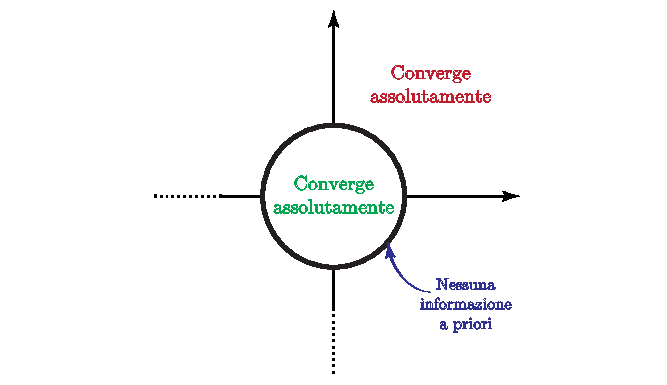
\includegraphics[trim=2.5cm 0.5cm 2.5cm 0cm, clip, scale=1]{images/discoconvergenza.pdf}
	\end{center}
\end{define}
Poiché sappiamo che la serie converge assolutamente per $\abs{z}<r$, lo studio del raggio di convergenza passa attraverso lo studio della serie assoluta associata $\displaystyle\sum_{n=0}^{+\infty}\abs{a_nz^n}$.\\
Per determinare il raggio di convergenza, possiamo ad esempio usare la \textbf{legge di D’Alembert}\seeonlyindex{criterio!del rapporto}{legge!di D’Alembert} o detto anche \textit{criterio del rapporto}\index{criterio!del rapporto}, che ci fornisce una condizione \textit{sufficiente} su come determinare il raggio di convergenza.
\begin{proposition}[Legge di D’Alembert o criterio del rapporto.]~{}\\
	Data la serie $\displaystyle\sum_{n=0}^{+\infty}a_nz^n$, se $a_n\neq 0$ definitivamente ed esiste il limite
	\begin{equation*}
		\lim_{n\to+\infty}\frac{\abs{a_{n+1}}}{\abs{a_{n}}}=L
	\end{equation*}
	allora
	\begin{enumerate}
		\item $L=0\implies R=+\infty$
		\item $L=+\infty\implies R=0$
		\item $0<L<+\infty\implies R=\frac{1}{L}$
	\end{enumerate}
\end{proposition}
Questa proposizione ha il vantaggio di essere operativamente utile, ma ovviamente solo se valgono le ipotesi: non è scontato che il limite del rapporto sia ben definito!\\
Un teorema più generale che vale \textit{per ogni serie} è il \textit{criterio della radice}\index{criterio!della radice} o altresì noto come \textbf{legge di Cauchy-Hadamard}\seeonlyindex{criterio!del rapporto}{legge!di Cauchy-Hadamard}.
\begin{theorema}
	Sia data la serie di potenze
	\begin{equation*}
		\sum_{n=0}^{+\infty}a_nz^n
	\end{equation*}
	e sia
	\begin{equation}
		\lambda=\limsup_{n\to+\infty}\sqrt[n]{\abs{n}}
	\end{equation}
	Allora
	\begin{enumerate}
		\item Se $\lambda = 0$, la serie converge $\forall z\in\complexset$.
		\item Se $0<\lambda<+\infty$, la serie converge $R=\frac{1}{\lambda}$.
		\item Se $\lambda = +\infty$, la serie converge solo in $z=0$.
	\end{enumerate}
\end{theorema}
\begin{observe}
	I tre casi scritti esauriscono \textit{tutti} i casi possibili. Infatti, per la permanenza del segno del limsup\footnote{Nelle ‘‘Note aggiuntive'', a pagina XXX è possibile trovare la dimostrazione di questo risultato insieme ad altri relativi al limsup e liminf.} vale
	\begin{equation*}
		\sqrt[n]{\abs{a_n}}\geq 0,\ \forall n\geq 0\implies\limsup_{n\to+\infty}\sqrt[n]{\abs{a_n}}\geq 0
	\end{equation*}
\end{observe}
\begin{demonstration}\textsc{(della legge di Cauchy-Hadamard.)}~{}\\
	Partiamo dal dimostrare il punto $2)$: dobbiamo provare che $R=\frac{1}{\lambda}$, ossia
	\begin{itemize}
		\item Se $\abs{z}<\nicefrac{1}{\lambda}$, allora $\displaystyle\sum_{n=0}^{+\infty}a_nz^n$ converge.
		\item Se $\abs{z}>\nicefrac{1}{\lambda}$, allora $\displaystyle\sum_{n=0}^{+\infty}a_nz^n$ \textit{non} converge.
	\end{itemize}
	\begin{itemize}
		\item Sia $z$ tale che $\abs{z}<\nicefrac{1}{\lambda}$. Se $z=0$ la serie banalmente converge.\\
		Se $z\neq 0$, vale $\lambda<\nicefrac{1}{\abs{z}}$; consideriamo allora $\lambda'$ tale che $\lambda<\lambda'<\nicefrac{1}{\abs{z}}$: poiché $\lambda'>\lambda$, per la caratterizzazione del massimo limite si ha
		\begin{equation*}
			\textcolor{red}{\circled{\ast}}\quad\exists N\colon\forall n\geq N\ \sqrt[n]{\abs{a_n}}<\lambda'
		\end{equation*}
		Proviamo che $\displaystyle\sum_{n=0}^{+\infty}a_nz^n$ converge assolutamente usando il criterio del confronto.
		\begin{equation*}
			\abs{a_nz^n}=\abs{a_n}\abs{z^n}=\abs{a_n}\abs{z}^n\substack{<}_{\textcolor{red}{\circled{\ast}}}<\left(\lambda'\right)^n\abs{z}^n=\left(\lambda'\abs{z}\right)^n,\ \forall n\geq N
		\end{equation*}
		Questo è il termine $n$-esimo della serie geometrica $\displaystyle\sum_{n=0}^{+\infty}\left(\lambda'\abs{z}\right)^n$ di ragione $\lambda'\abs{z}$.\\
		Poiché $0<\lambda'\abs{z}<1$ per la scelta di $\lambda'$, la serie geometrica converge e quindi per il criterio del confronto converge anche la serie $\displaystyle\sum_{n=0}^{+\infty}\abs{a_nz^n}$ e dunque converge anche $\displaystyle\sum_{n=0}^{+\infty}a_nz^n$.
		\item Sia $z$ tale che $\abs{z}>\nicefrac{1}{\lambda}$. Per mostrare la non convergenza della serie proviamo che la condizione necessaria di convergenza non è soddisfatta, ovvero
		\begin{equation*}
			\lim_{n\to+\infty}a_nz^n\neq 0,\ \forall z\colon \abs{z}>\frac{1}{\lambda}
		\end{equation*}
		Questo è equivalente a mostrare che
		\begin{equation*}
			\lim_{n\to+\infty}\abs{a_nz^n}\neq 0,\ \forall z\colon \abs{z}>\frac{1}{\lambda}
		\end{equation*}
		Poiché $z\neq 0$, vale $\lambda>\nicefrac{1}{\abs{z}}$.	Consideriamo allora $\lambda''$ tale che $\nicefrac{1}{\abs{z}}<\lambda''<\lambda$: poiché $\lambda''<\lambda$, per la caratterizzazione del massimo limite si ha
		\begin{equation*}
			\textcolor{blue}{\circled{\ast}}\quad\exists n_k\to+\infty\colon\sqrt[n_k]{\abs{a_{n_k}}}>\lambda''
		\end{equation*}
		Si ha, lungo la sottosuccessione:
		\begin{equation*}
			\abs{a_{n_k}z^{n_k}}=\abs{a_n}{z}^{n_k}\substack{>}_{\textcolor{blue}{\circled{\ast}}}>\left(\lambda''\right)^{n_k}\abs{z}^{n_k}=\left(\substack{\lambda''\abs{z}}_{>1\text{ per la scelta di }\lambda''}\right)^{n_k}>1,\ \forall n_k
		\end{equation*}
		Poiché esiste una sottosuccessione che è sempre maggiore di $1$, deve esistere un valore limite della successione $\abs{a_nz^n}$ maggiore o uguale a $1$. Ma allora
		\begin{equation*}
			\limsup_{n\to+\infty}\abs{a_nz^n}\geq 1\implies\lim_{n\to+\infty}\abs{a_nz^n}\neq 0
		\end{equation*}
	\end{itemize}
	La dimostrazione del punto $1)$ è analoga alla prima parte della dimostrazione del punto $2)$. In questo caso, dobbiamo mostrare che la serie converge $\forall z\in\complexset$.\\ Se $z=0$, la serie banalmente converge, mentre se $z\neq 0$, si ha chiaramente che $0=\lambda<\nicefrac{1}{\abs{z}},\ \forall z\in\complexset\setminus\{0\}$. Consideriamo allora $\lambda'$ tale che $0<\lambda'<\nicefrac{1}{\abs{z}}$: poiché $\lambda'>0$, per la caratterizzazione del massimo limite si ha
	\begin{equation*}
		\textcolor{red}{\circled{\ast}}\quad\exists N\colon\forall n\geq N\ \sqrt[n]{\abs{a_n}}<\lambda'
	\end{equation*}
	Proviamo che $\displaystyle\sum_{n=0}^{+\infty}a_nz^n$ converge assolutamente usando il criterio del confronto.
	\begin{equation*}
		\abs{a_nz^n}=\abs{a_n}\abs{z^n}=\abs{a_n}\abs{z}^n\substack{<}_{\textcolor{red}{\circled{\ast}}}<\left(\lambda'\right)^n\abs{z}^n=\left(\lambda'\abs{z}\right)^n,\ \forall n\geq N
	\end{equation*}
	Questo è il termine $n$-esimo della serie geometrica $\displaystyle\sum_{n=0}^{+\infty}\left(\lambda'\abs{z}\right)^n$ di ragione $\lambda'\abs{z}$.\\
	Poiché $0<\lambda'\abs{z}<1$ per la scelta di $\lambda'$, la serie geometrica converge e quindi per il criterio del confronto converge anche la serie $\displaystyle\sum_{n=0}^{+\infty}\abs{a_nz^n}$ e dunque converge anche $\displaystyle\sum_{n=0}^{+\infty}a_nz^n$. Poiché la scelta di $z$ è stata arbitraria, vale la tesi.\\
	La dimostrazione del punto $1)$ è analoga alla seconda parte della dimostrazione del punto $2)$. In questo caso, dobbiamo mostrare che la serie converge solo in $z=0$.\\ Se $z=0$, la serie banalmente converge. Per mostrare la non convergenza della serie proviamo che la condizione necessaria di convergenza non è soddisfatta, ovvero
	\begin{equation*}
		\lim_{n\to+\infty}a_nz^n\neq 0,\ \forall z\neq 0
	\end{equation*}
	Questo è equivalente a mostrare che
	\begin{equation*}
		\lim_{n\to+\infty}\abs{a_nz^n}\neq 0,\ \forall z\neq 0
	\end{equation*}
	Dato $z\neq 0$, consideriamo allora $\lambda''$ tale che $\nicefrac{1}{\abs{z}}<\lambda''<+\infty$: poiché $\lambda''<+\infty$, per la caratterizzazione del massimo limite si ha
	\begin{equation*}
		\textcolor{blue}{\circled{\ast}}\quad\exists n_k\to+\infty\colon\sqrt[n_k]{\abs{a_{n_k}}}>\lambda''
	\end{equation*}
	Si ha, lungo la sottosuccessione:
	\begin{equation*}
		\abs{a_{n_k}z^{n_k}}=\abs{a_n}{z}^{n_k}\substack{>}_{\textcolor{blue}{\circled{\ast}}}>\left(\lambda''\right)^{n_k}\abs{z}^{n_k}=\left(\substack{\lambda''\abs{z}}_{>1\text{ per la scelta di }\lambda''}\right)^{n_k}>1,\ \forall n_k
	\end{equation*}
	Poiché esiste una sottosuccessione che è sempre maggiore di $1$, deve esistere un valore limite della successione $\abs{a_nz^n}$ maggiore o uguale a $1$. Ma allora
	\begin{equation*}
		\limsup_{n\to+\infty}\abs{a_nz^n}\geq 1\implies\lim_{n\to+\infty}\abs{a_nz^n}\neq 0
	\end{equation*}
	La scelta di $z$ è arbitraria, purché $z$ sia diverso da zero; per questo motivo vale la tesi.
\end{demonstration}
\section{Comportamento sul bordo}
Consideriamo la serie di potenze
\begin{equation*}
	\sum_{n=0}^{+\infty}a_nz^n,\quad a_n,\ z\in\complexset
\end{equation*}
con raggio di convergenza finito e non nullo.
I possibili comportamenti sul \textit{bordo} del cerchio di convergenza sono i seguenti:
\begin{enumerate}
	\item Convergenza in \textit{tutti i punti} del bordo del cerchio di convergenza
	\item \textit{Non} convergenza in \textit{nessun punto} del bordo del cerchio di convergenza
	\item Convergenza solo in \textit{alcuni punti} del bordo del cerchio di convergenza
\end{enumerate}
Mostriamo per ciascuno di essi un esempio.
\begin{example}\textsc{Caso 1.}~{}\\
	Consideriamo la serie
	\begin{equation*}
		\sum_{n=1}^{+\infty}\frac{z^n}{n^\alpha},\quad\alpha>1
	\end{equation*}
	Con la formula di D'Alembert vediamo che il raggio di convergenza è $R=1$. Infatti
	\begin{equation*}
		\lim_{n\to+\infty}\frac{\abs{a_{n+1}}}{\abs{a_{n}}}=\lim_{n\to+\infty}\frac{\left(n+1\right)^\alpha}{n^\alpha}=\lim_{n\to+\infty}\frac{n^\alpha\left(1+\frac{1}{n}\right)^\alpha}{n^\alpha}=\lim_{n\to+\infty}\left(1+\frac{1}{n}\right)^\alpha=1=\mathcal{l}\implies r=\frac{1}{\mathcal{l}}=1
	\end{equation*}
	Per ogni $z\in\complexset$ tale che $\abs{z}=1$ la serie converge (assolutamente):
	\begin{equation*}
		\sum_{n=1}^{+\infty}\abs{\frac{z^n}{n^\alpha}}=\sum_{n=1}^{+\infty}\frac{n}{n^\alpha}
	\end{equation*}
	La serie in modulo è la \textit{serie armonica generalizzata} che, per $\alpha>1$, converge; la serie semplice converge su tutti i punti del bordo.
\end{example}
\begin{example}\textsc{Caso 2.}~{}\\
	Consideriamo la \textit{serie geometrica}
	\begin{equation*}
		\sum_{n=1}^{+\infty}z^n
	\end{equation*}
	Poichè $a_n\equiv 1\ \forall n$, il criterio del rapporto ci fornisce come raggio di convergenza $R=1$.\\
	Per ogni $z\in\complexset$ tale che $\abs{z}=1$ la serie \textit{non} converge: possiamo osservare che presa la successione $c_n\in\complexset$, vale\footnote{Nelle ‘‘Note aggiuntive'', a pagina XXX è possibile trovare la dimostrazione di questo risultato.}
	\begin{equation*}
		\lim_{n\to+\infty}\abs{c_n}\neq 0\implies\lim_{n\to+\infty}c_n\neq 0
	\end{equation*}
	In questo caso:
	\begin{equation*}
		\lim_{n\to+\infty}\abs{z^n}=\lim_{n\to+\infty}1=1\neq 0\implies\lim_{n\to+\infty}z^n\neq 0
	\end{equation*}
	È evidente che la \textit{condizione necessaria} di convergenza \textit{non} è soddisfatta: la serie \textit{non} converge in nessun punto del bordo.
\end{example}
\begin{example}\textsc{Caso 3.}~{}\\
	Consideriamo la serie
	\begin{equation*}
		\sum_{n=1}^{+\infty}\frac{z^n}{n^\alpha},\quad0<\alpha<1
	\end{equation*}
	L'applicazione del criterio del confronto è esattamente analogo a quello visto nel caso  e il raggio di convergenza è pertanto $R=1$.\\
	Se $z=1$ la serie \textit{non} converge, dato che essa diventa una serie armonica generalizzata con $\alpha\leq1$:
	\begin{equation*}
		\sum_{n=1}^{+\infty}\frac{1}{n^\alpha}
	\end{equation*}
	Invece, per ogni $z\in\complexset$ tale che $\abs{z}=1$ e $z\neq 1$ la serie converge: infatti, possiamo applicare il \textit{criterio di Abel-Dirichlet}.
	\begin{equation*}
		\sum_{n=1}^{+\infty}\frac{z^n}{n^\alpha}=\sum_{n=1}^{+\infty}z^n\frac{1}{n^\alpha}=\sum_{n=1}^{+\infty}\alpha_n\beta_n
	\end{equation*}
	con $\alpha_n=z^n$ e $\beta_n=\nicefrac{1}{n^\alpha},\ n\geq 1$.
	\begin{enumerate}
		\item $\beta_n=\nicefrac{1}{n^\alpha}$ è una successione di elementi strettamente positivi, decrescenti e infinitesima per $n\to+\infty$.
		\item La successione delle \textit{somme parziali} di $\alpha_n=z^n$ è \textit{limitata}. Consideriamo
		\begin{equation*}
			\abs{\sum_{n=1}^{k}z^n}=\abs{\sum_{n=0}^{k}z^n-1}\squarequal
		\end{equation*}
		Poiché $\displaystyle\sum_{n=0}^{k}z^n$ è un serie geometrica parziale, sappiamo la sua somma parziale. Applicando poi una \textit{disuguaglianza triangolare}, troviamo una \textit{maggiorazione} della somma parziale di $\alpha_n$.
		\begin{equation*}
			\squarequal\abs{\frac{1-z^{k+1}}{1-z}-1}=\abs{\frac{z-z^{k+1}}{1-z}}\leq\frac{\abs{z}+\abs{-z^{k+1}}}{\abs{1-z}}\leq\frac{1+1}{\abs{1-z}}=\frac{2}{\abs{1-z}},\ \forall k\geq 1
		\end{equation*}
	\end{enumerate}
	Osserviamo che, nonostante la serie converga, essa non converge assolutamente: la serie in modulo è la serie armonica generalizzata con $\alpha\leq 1$, nota per essere divergente.
\end{example}
Anche se in generale non possiamo affermare a priori come converge sul bordo si può osservare che, in alcuni casi particolari, dalla converge in un punto del bordo si ottiene la convergenza sull'intero bordo. Vediamone alcuni
\begin{proposition}[Convergenza assoluta sul bordo se la serie di potenze converge assolutamente in un punto.]~{}\\
	Sia data la serie di potenze
	\begin{equation*}
		\sum_{n=1}^{+\infty}a_nz^n
	\end{equation*}
	Se la serie converge assolutamente in un punto della frontiera del cerchio di convergenza, allora converge assolutamente su tutta questa frontiera.
\end{proposition}
\begin{demonstration}
	Supponiamo che la serie converga assolutamente in $z_0$, dove $\abs{z_0}=R$ e prendiamo un qualunque $z$ tale che $\abs{z}=R$.
	Osserviamo che, presa la serie in modulo, si ha
	\begin{equation*}
		\sum_{n=1}^{+\infty}\abs{a_nz^n}=\sum_{n=1}^{+\infty}\abs{a_n}\abs{z^n}=\sum_{n=1}^{+\infty}\abs{a_n}\abs{z}^n=\sum_{n=1}^{+\infty}\abs{a_n}R^n=\sum_{n=1}^{+\infty}\abs{a_n}ì\abs{z_0}^n=\sum_{n=1}^{+\infty}\abs{a_nz_0^n}
	\end{equation*}
	che converge per ipotesi. Allora la serie di potenze converge assolutamente.
\end{demonstration}
\begin{corollary}[Convergenza sul bordo se la serie di potenze a coefficienti reali positivi converge in $z=R$.]~{}\\
	Sia data la serie di potenze
	\begin{equation*}
		\sum_{n=1}^{+\infty}a_nz^n
	\end{equation*}
	Se la serie ha coefficienti reali positivi e converge nel punto $z=R$, dove $R\in\left(0,+\infty\right)$ è il raggio di convergenza, allora converge in ogni punto della frontiera del cerchio di convergenza.
\end{corollary}
\begin{demonstration}
	Poiché $a_n$ e $R$ sono reali positivi, $a_n=\abs{a_n}$ e $R=\abs{R}$. Allora si ha
	\begin{equation*}
		\sum_{n=1}^{+\infty}a_nR^n=\sum_{n=1}^{+\infty}\abs{a_nR^n}
	\end{equation*}
	Quindi in questo caso la convergenza semplice della serie implica la convergenza assoluta. Poiché la serie converge assolutamente in un punto del bordo, segue dalla proposizione precedente la convergenza (assoluta) in tutti i punti del bordo.
\end{demonstration}
\section{Serie di potenze e convergenza uniforme}
\begin{theorema}[Converge uniforme delle serie di potenze.]~{}\\\label{convergenzasottoinsiemeH}
	Sia $\displaystyle\sum_{n=0}^{+\infty}a_nz^n$ una serie di potenze con raggio di convergenza $R\in\left(0,+\infty\right)$. Allora
	\begin{enumerate}
		\item La serie converge uniformemente su ogni insieme $H\subseteq\complexset$ tale che $\overline{H}\subsetneqq B_R\left(0\right)$, con $B_R\left(0\right)$ il disco aperto di convergenza.
		\item Se la serie converge assolutamente in ogni $z\in\partial B_R\left(0\right)$ (il bordo del disco), allora converge uniformemente sul disco chiuso $\overline{B_R\left(0\right)}$.
	\end{enumerate}
\end{theorema}
\begin{demonstration} Per questa dimostrazione useremo il \textit{criterio di Weierstrass} enunciato nella sezione \ref{criteriodiweierstrass}, pag. \pageref{criteriodiweierstrass}.
	\begin{enumerate}
		\item Sia $H$ tale che $\overline{H}\subsetneqq B_R\left(0\right)$. Per il criterio di Weierstrass, per provare la convergenza uniforme su $H$ è sufficiente provare che esiste una successione $c_n$ tale che
		\begin{enumerate}
			\item $\abs{a_nz^n}\leq c_n,\ \forall z\in H$
			\item $\displaystyle\sum_{n=0}^{+\infty}c_n$ converge.
		\end{enumerate}
		\begin{minipage}{0.40\textwidth}
			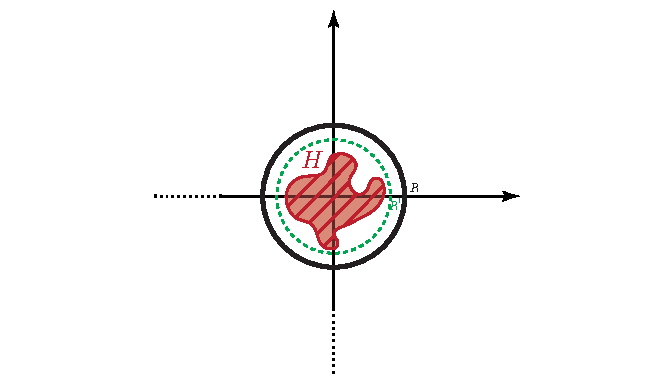
\includegraphics[trim=0cm 0cm 0cm 0cm, clip, scale=1]{images/discoconvergenzainsiemeH.pdf}
		\end{minipage}\hspace{-7mm}
		\begin{minipage}{0.55\textwidth}
			Poiché $H$ è solo \textit{strettamente contenuto} nel disco aperto di convergenza, $\exists R'<R$ tale che si abbia $\overline{H}\subseteq B_{R'}\left(0\right)$, ossia $\abs{z}\leq R',\ \forall z\in H$.\\
			Allora si ha, $\forall n\geq 0$ e $\forall z\in H$
			\begin{equation*}
				\abs{a_nz^n}=\abs{a_n}\abs{z}^n\leq \underbrace{\abs{a_n}\left(R'\right)^n}_{\text{non dipende da }z}
			\end{equation*}
		\end{minipage}\\
		Inoltre, la serie $\displaystyle\sum_{n=0}^{+\infty}c_n=\sum_{n=0}^{+\infty}\abs{a_n}\left(R'\right)^n$ converge in quanto è la convergenza della serie di potenze per il punto $z=R'$, che è \textit{interno} al disco di convergenza $B_R\left(0\right)$. Applicando il criterio di Weierstrass otteniamo la tesi.
		\item Si ripete la dimostrazione sull'insieme $\overline{B_R\left(0\right)}$ con $R'=R$, considerando che la serie $\displaystyle\sum_{n=0}^{+\infty}\abs{a_n}R^n$ converge per ipotesi sulla convergenza sul bordo.
	\end{enumerate}
\end{demonstration}
\begin{example}\textsc{Serie geometrica.}\\
	Sulla \textit{serie geometrica} $\displaystyle\sum_{n=0}^{+\infty}z^n$ abbiamo già ricavato diverse informazioni: ha raggio di convergenza $R=1$ e \textit{non} c'è convergenza (assoluta) sul bordo. Studiamo ora la convergenza uniforme.
	\begin{itemize}
		\item Converge uniformemente su ogni insieme $H$ tale che $\overline{H}\subsetneqq B_1\left(0\right)$ per il teorema precedente.
		\item Non avendo alcuna convergenza sul bordo, a priori non possiamo dare risultati generali sulla convergenza uniforme sulla base del teorema visto. Tuttavia, possiamo mostrare direttamente - grazie al fatto che la somma parziale e limite della serie geometrica è nota\footnote{Nelle ‘‘Note aggiuntive'', a pagina XXX è possibile trovare maggiori dettagli sulla somma (parziale) della serie geometrica e come ricavarla.} -  che la serie non converge uniformemente sul disco aperto $B_1\left(0\right)$. Infatti
		\begin{align*}
			\sup_{z\in B_1\left(0\right)}\abs{S_n\left(z\right)-S\left(z\right)}&=\sup_{z\in B_1\left(0\right)}\abs{\frac{1-z^{n+1}}{1-z}-\frac{1}{1-z}}=\sup_{z\in B_1\left(0\right)}\abs{\frac{-z^{n+1}}{1-z}}=\\
			&=\sup_{z\in B_1\left(0\right)}\frac{\abs{z}^{n+1}}{\abs{1-z}}=+\infty,\ \forall n\geq 0
		\end{align*}
		da cui
		\begin{equation*}
			\lim_{n\to+\infty}\left(\sup_{z\in B_1\left(0\right)}\abs{S_n\left(z\right)-S\left(z\right)}\right)=+\infty\neq 0
		\end{equation*}
	\end{itemize}
\end{example}
\section{Proprietà di regolarità della somma di una serie di potenze}
Sia $\displaystyle\sum_{n=0}^{+\infty}a_nz^n$ una serie di potenze con $R>0$ il raggio di convergenza. Studiamo le proprietà di continuità e derivabilità della \textbf{funzione somma}\index{funzione!somma}
\begin{equation}
	\funztot{f}{B_R\left(0\right)\subseteq\complexset}{\complexset}{z}{\displaystyle\sum_{n=0}^{+\infty}a_nz^n}
\end{equation}
\subsection{Continuità}
\begin{proposition}[Proprietà di continuità per la somma di una serie di potenze, caso generale.]~{}\\
	La funzione $f$ è continua su $B_R\left(0\right)$.
\end{proposition}
\begin{attention}
	La convergenza della serie di potenze su $B_R\left(0\right)$ \textit{non} è in generale uniforme, ma sappiamo al più che converge uniformemente su $H$ tale che $\overline{H}\subsetneqq B_R\left(0\right)$, quindi dobbiamo tenere conto di questo fattore nelle dimostrazioni che faremo.
\end{attention}
\begin{demonstration}
	Dobbiamo provare che $f\in\mathcal{C}\left(B_R\left(0\right)\right)$, cioè $f$ continua in $z_0,\ \forall z_0\in B_R\left(0\right)$.	\vspace{3mm}
	\begin{minipage}{0.44\textwidth}
		\includegraphics[trim=0cm 0cm 0cm 0cm, clip, scale=1.1]{images/discoconvergenzacontinuitaf.pdf}
	\end{minipage}\hspace{-9mm}
	\begin{minipage}{0.60\textwidth}
		Sia $z_0\in B_R\left(0\right)$ fissato. Per proprietà della metrica, allora $\exists R_0 < R$ tale che $z_0\in B_{R_0}\left(0\right)$. Su $B_{R_0}\left(0\right)$ si ha continuità uniforme e dunque, posto
		\begin{equation*}
			S_n\left(z\right)=\sum_{k=0}^{n}a_kz^k
		\end{equation*}
		si ha
		\begin{enumerate}
			\item $S_n$ continua su $B_{R_0}\left(0\right)$ perché è un polinomio.
			\item $S_n$ converge uniformemente a $f$ su $B_R\left(0\right)$.
		\end{enumerate}
	\end{minipage}\\
	Per il teorema di continuità della funzione limite, $f$ è continua in $B_{R_0}\left(0\right)$ e dunque in $z_0$. 
\end{demonstration}
Questo risultato ci permette di parlare della convergenza sul disco aperto, ma se c'è qualche tipo di convergenza sul bordo, e quindi $f$ è definita anche su di esso, si può estendere la continuità di $f$ fino a tale frontiera? Studiamo due casi.
\begin{corollary}[Proprietà di continuità per la somma di una serie di potenze, caso sul bordo con convergenza assoluta.]~{}\\
	Sia data la serie di potenze $\displaystyle\sum_{n=0}^{+\infty}a_nz^n$ con raggio di convergenza $R>0$. Se la serie converge (assolutamente) su $\partial B_R\left(0\right)$ allora la serie è continua su $\overline{B_R\left(0\right)}$.
\end{corollary}
\begin{demonstration}
	Segue immediatamente ricordando che dalle ipotesi di convergenza assoluta sul bordo, sulla base del teorema \ref{convergenzasottoinsiemeH}, pag. \pageref{convergenzasottoinsiemeH}, vale la convergenza uniforme su $\overline{B_R\left(0\right)}$.
\end{demonstration}
Se invece supponiamo che la serie converga in un punto\footnote{Nel caso di più punti di convergenza $z_0,\ z_1,\ \ldots$, la funzione somma $f$ sarà definita su $B_R\left(0\right)\cup\left\{z_0\right\}\cup\left\{z_1\right\}\cup\ldots$. Qui riportiamo per semplicità il caso di un solo punto, ma i risultati successivi sono opportunamente generalizzabili con più punti di convergenza sul bordo.} $z_0$, cioè $\displaystyle\sum_{n=0}^{+\infty}a_nz_0^n$ converge, possiamo definire la \textbf{funzione somma}\index{funzione!somma} come
\begin{equation}
	\funztot{f}{B_R\left(0\right)\cup\left\{z_0\right\}\subseteq\complexset}{\complexset}{z}{\displaystyle\sum_{n=0}^{+\infty}a_nz^n}
\end{equation}
La convergenza uniforme di $f$ anche sui punti di convergenza $z_0$ sul bordo ci viene garantita dal \textbf{teorema di Abel}\index{teorema!di Abel}.
\begin{theorema}[Teorema di Abel.]~{}\\
	Sia dato la serie di potenze la serie di potenze $\displaystyle\sum_{n=0}^{+\infty}a_nz^n$ con raggio di convergenza $R>0$. Se $\exists z_0=Re^{i\theta_0}$ tale che $\displaystyle\sum_{n=0}^{+\infty}a_nz_0^n$ converge, allora\\
	\begin{minipage}{0.39\textwidth}
		\includegraphics[trim=0cm 0cm 0cm 0cm, clip, scale=1]{images/discoconvergenzaabel.pdf}
	\end{minipage}\hspace{-12mm}
	\begin{minipage}{0.65\textwidth}
		\begin{enumerate}
			\item la serie converge uniformemente sul \textit{segmento}
			\begin{equation}
				\Sigma_0=\left\{z\in\complexset\mid z=re^{i\theta_0},\ r\in\left[0,R\right]\right\}
			\end{equation}
			\item La restrizione di $f$ a $\Sigma_0$ è \textit{continua} su $z_0$, ossia
			\begin{equation}
				\lim_{r\to R}f\left(re^{i\theta_0}\right)=f\left(z_0\right)=\sum_{n=0}^{+\infty}a_nz_0^n
			\end{equation}
		\end{enumerate}
	\end{minipage}
\end{theorema}
\subsection{Derivabilità}
Abbiamo definito la funzione somma dal disco aperto $B_R\left(0\right)$ in campo complesso a $\complexset$, ma al momento non conosciamo cosa vuol dire derivabilità di una funzione $\funz{f}{\complexset}{\complexset}$. Per il momento, limitiamoci al caso reale, cioè consideriamo una serie di potenze
\begin{equation*}
	\sum_{n=0}^{+\infty}a_nx^n,\ x\in\realset,\ a_n\in\realset
\end{equation*}
con raggio di convergenza $R>0$. In questo caso il cerchio di convergenza è un intervallo $\left(-R,R\right)$, con estremi eventualmente inclusi. La funzione somma risulta allora la funzione
\begin{equation}
	\funztot{f}{\left(-R,R\right)}{\realset}{x}{\sum_{n=0}^{+\infty}a_nx^n}
\end{equation}
\begin{theorema}[Derivabilità della somma di una serie di potenze.]~{}\\
	Sia data
	\begin{equation*}
		f\left(x\right)=\sum_{n=0}^{+\infty}a_nx^n,\ \forall x\in\left(-R,R\right),\ a_n\in\realset
	\end{equation*}
con $R>0$ il raggio di convergenza. Allora
\begin{enumerate}
	\item $f$ è derivabile su $\left(-R,R\right)$
	\item La derivata di $f$ è
	\begin{equation}
		f'\left(x\right)=\sum_{n=1}^{+\infty}na_nx^{n-1},\ \forall x\in\left(-R,R\right)
	\end{equation}
\end{enumerate}
\end{theorema}
Per dimostrare questo teorema useremo il teorema di derivibilità per serie di funzioni (teorema \ref{derivabilitatermineatermine}, pag. \pageref{derivabilitatermineatermine}, capitolo \refChapter{seriefunzioni}): poiché le ipotesi $1)$ e $2)$ sono banalmente verificate, dobbiamo contrarci sull'ipotesi $3)$, ovvero abbiamo bisogno di informazioni sulla convergenza uniforme della serie delle derivate $\displaystyle\sum_{n=1}^{+\infty}na_nx^{n-1}$; poiché la serie delle derivate è ancora una serie di potenze, allora ci basta studiare il raggio di convergenza.
% TO DO: nelle Note extra a pagina XXX inserire il prodotto del lim sup
\begin{lemming}[Convergenza della serie di derivate della serie di potenze.]~{}\\
	Sia data la serie di potenze $\displaystyle\sum_{n=0}^{+\infty}a_nx^n$ e sia $R>0$ il suo raggio di convergenza. Allora la serie di potenze $\displaystyle\sum_{n=1}^{+\infty}na_nx^{n-1}$ ha raggio di convergenza $R$.
\end{lemming}
\begin{demonstration}
	Riscriviamo la serie delle derivate, operando un cambio di indici ponendo $n=k+1$
	\begin{equation*}
		\sum_{n=1}^{+\infty}na_nx^{n-1}=\sum_{k=0}^{+\infty}\underbrace{\left(k+1\right)a_{k+1}}_{=b_k}x^k=\sum_{k=0}^{+\infty}b_ka_k
	\end{equation*}
	Sia $R'$ il suo raggio di convergenza. Per il teorema di Cauchy-Hadamard si ha
	\begin{equation*}
		\frac{1}{R'}=\limsup_{n\to+\infty}\abs{b_n}^{\nicefrac{1}{n}}=\limsup_{n\to+\infty}\abs{\left(n+1\right)a_{n+1}}^{\nicefrac{1}{n}}=\limsup_{n\to+\infty}\underbrace{\left(n+1\right)^{\nicefrac{1}{n}}}_{=\alpha_n}\underbrace{\abs{a_{n+1}}^{\nicefrac{1}{n}}}_{=\beta_n}=\limsup_{n\to+\infty}\alpha_n\beta_n\squarequal
	\end{equation*}
Osserviamo che
\begin{equation*}
	\lim_{n\to+\infty}\alpha_n=\lim_{n\to+\infty}\left(n+1\right)^{\nicefrac{1}{n}}=\lim_{n\to+\infty}e^{\frac{1}{n}\log\left(n+1\right)}=\lim_{n\to+\infty}e^{\frac{\log\left(n+1\right)}{n}}
\end{equation*}
Poichè $\frac{\log\left(n+1\right)}{n}\to 0$ per $n\to+\infty$ per confronto della crescita degli infiniti, $\displaystyle\lim_{n\to+\infty}\alpha_n=e^0=1$, dunque $\alpha_n$ ammette limite e dunque coincide col suo $\limsup$. Allora, per proprietà\footnote{Nelle ‘‘Note aggiuntive'', a pagina XXX è possibile trovare la dimostrazione di questo risultato insieme ad altri relativi al limsup e liminf.} del $\limsup$:
\begin{equation*}
	\squarequal\lim_{n\to+\infty}\alpha_n\limsup_{n\to+\infty}\beta_n=\limsup_{n\to+\infty}\abs{a_{n+1}}^{\nicefrac{1}{n}}=\limsup_{n\to+\infty}\left(\abs{a_{n+1}}^{\nicefrac{1}{n+1}}\right)^{\nicefrac{n+1}{n}}\squarequal
\end{equation*}
Poichè $\nicefrac{n+1}{n}\to 1$ per $n\to+\infty$, possiamo applicare Cauchy-Hadamar sulla serie di potenze $\displaystyle\sum_{n=0}^{+\infty}a_nx^n$ con raggio di convergenza $R>0$: poiché
\begin{equation*}
	\frac{1}{R}=\limsup_{n\to+\infty}\abs{a_n}^{\nicefrac{1}{n}}=\limsup_{n\to+\infty}\abs{a_{n+1}}^{\nicefrac{1}{n+1}}
\end{equation*}
allora abbiamo mostrato che
\begin{equation*}
	\frac{1}{R'}=\ldots=\limsup_{n\to+\infty}\left(\abs{a_{n+1}}^{\nicefrac{1}{n+1}}\right)^{\nicefrac{n+1}{n}}=\frac{1}{R}
\end{equation*}
cioè $R'=R$.
\end{demonstration}
Grazie a questo lemma, possiamo finalmente dimostrare il teorema lasciato in sospeso all'inizio della sezione.
\begin{demonstration}\textsc{(del Teorema di derivabilità della somma di una serie di potenze.)}\\
	Fissiamo $\overline{x}\in\left(-R,R\right)$ arbitrario e sia $\left(a,b\right)$ tale che
	\begin{itemize}
		\item $\overline{x}\in\left(a,b\right)$.
		\item $\left[a,b\right]\subsetneqq\left(-R,R\right)$
	\end{itemize}
Applichiamo ora il teorema di derivabilità termine a termine della serie di funzioni su $\left(a,b\right)$ sulla serie di potenze $\displaystyle\sum_{n=0}^{+\infty}a_nx^n$; vediamo che le ipotesi sono verificate:
\begin{itemize}
	\item $f_n\left(x\right)=a_nx^n$ derivabile in $\left(a,b\right),\ \forall n\geq 1$.
	\item $\displaystyle\sum_{n=0}^{+\infty}f_n\left(x\right)$ converge $\forall x\in\left(a,b\right)$
	\item $\displaystyle\sum_{n=1}^{+\infty}f'_n\left(x\right)=\sum_{n=1}^{+\infty}na_nx^{n-1}$ converge uniformemente su $\left(a,b\right)$ per la scelta di $\left(a,b\right)$, sulla base del lemma precedentemente dimostrato.
\end{itemize}
Per il teorema di derivabilità termine a termine $f$ è derivabile in $\left(a,b\right)$ e dunque anche in $\overline{x}$, con derivata in tal punto
\begin{equation*}
	f'\left(\overline{x}\right)=\sum_{n=1}^{+\infty}na_nx^{n-1}
\end{equation*}
Per l'arbitrarietà di $\overline{x}$, questi risultati valgono $\forall x\in\left(-R,R\right)$ e dunque segue la tesi.
\end{demonstration}
\section{Funzioni analitiche e serie di Taylor}
La tesi $2)$ appena dimostrata ci dice che la derivata $f'$ è una somma di serie di potenze con stesso raggio di convergenza $R$ di $f$. Possiamo riapplicare il teorema alla funzione $f'$:
\begin{itemize}
	\item $f'$ è derivabile in $\left(-R,R\right)$.
	\item $\displaystyle f''\left(x\right)=\sum_{n=2}^{+\infty}n\left(n-1\right)a_nx^{n-2},\ \forall x\in\left(-R,R\right)$.
\end{itemize}
Ma anche $f''$ è una serie di potenze con raggio $R$: possiamo riapplicare il teorema su $f''$ e ammettere l'esistenza di $f'''$ come serie di potenze. Iterando il ragionamento, si trova che esiste $f^{\left(k\right)}\left(x\right),\ \forall x\in\left(-R,R\right),\ \forall k\geq 0$ e vale
\begin{equation}
	f^{\left(k\right)}\left(x\right)=\sum_{n=k}^{+\infty}n\left(n-1\right)\ldots\left(n-k+1\right)a_nx^{n-k},\ \forall x\in\left(-R,R\right)
\end{equation}
\part{Teoria della misura e dell'integrazione}
\labelPart{second}
% SVN info for this file
\svnidlong
{$HeadURL$}
{$LastChangedDate$}
{$LastChangedRevision$}
{$LastChangedBy$}

\chapter{Teoria della misura}
\labelChapter{azionidigruppo}

\begin{introduction}
	‘‘BEEP BOOP QUESTA È UNA CITAZIONE.''
\begin{flushright}
	\textsc{Marinobot,} dopo aver finito le citazioni stupide.
\end{flushright}
\end{introduction}
\lettrine[findent=1pt, nindent=0pt]{S}{tudieremo} \textbf{[COMPLETARE]}
% TO DO: completare intro
\section{Il contesto storico: il problema delle discontinuità nell'integrale definito}
Seppur tecniche per calcolare aree e volumi furono già introdotte dai matematici dell'antica Grecia, fu solo nel tardo XVII secolo che vennero sviluppati i principi dell'integrazione indipendentemente da Isaac Newton (1643-1727) e Gottfried Wilhelm Leibniz (1646-1716), i quali immaginarono l'area sotto una curva come una \textit{somma infinita} di rettangoli di \textit{larghezza infinitesima}.\\
Nel corso dell'Ottocento una buona parte delle ricerche dell'Analisi si concentrarono su un aspetto dell'integrale definito di una funzione: \textit{quanti} possono essere i \textit{punti discontinuità} di una funzione
integrabile e, più in generale, quali \textit{classi} di funzioni sono integrabili?\\
Augustin-Louis Cauchy (1789-1857) in \textit{Résumé des leçons données à	l’École Royale Polytechnique sur le calcul infinitésimal (1823)} definì l'integrale per funzioni continue o con al più un numero finito di discontinuità.\\
Successivamente, fu Bernhard Riemann (1826-1866) nella sua \textit{Tesi di abilitazione all'insegnamento (1851-1852)} a estendere il concetto di integrale alle funzioni limitate e dare una caratterizzazione delle funzioni integrabili (ora dette \textbf{integrabili secondo Riemann}).
\begin{define}[Caratterizzazione degli integrali secondo Riemann]
La funzione $\funz{f}{\left[a,b\right]}{\realset}$ limitata è \textbf{integrabile} (secondo Riemann) se e solo se $\forall \epsilon>0,\ \exists D$ suddivisione di $\left[a,b\right]$ in un numero finito di intervalli $I_1,\ \ldots,\ I_n$ tale per cui
\begin{equation}
	\sum_{i=1}^{n}\left(\sup_{I_i}f-\inf_{I_i}f\right)\mathcal{L}\left(I_i\right)<\epsilon
\end{equation}
\end{define}
Dalla caratterizzazione di Riemann è evidente che affinché una funzione sia integrabile è necessario rendere \textit{piccola} l’\textit{oscillazione} di f, ossia
\begin{equation*}
	\sup_{I_i}f-\inf_{I_i}f
\end{equation*}
Dal teorema di \textit{Heine-Cantor} è noto che per le funzioni continue su $\left[a,b\right]$ questa oscillazione è arbitrariamente piccola se l’ampiezza dell’intervallo $I_i$ è
sufficientemente piccola, mentre in generale non lo è.
\begin{examplewt}[La funzione di Dirichlet]\label{funzionedirichlet}
	Consideriamo la \textbf{funzione di Dirichlet}\index{funzione!di Dirichlet}
	\begin{equation}
		f\left(x\right)=
		\begin{cases}
			\begin{array}{ll}
				1&\text{se }x\in\left[0,1\right]\cap\rationalset\\
				0&\text{se }x\in\left[0,1\right]\setminus\rationalset\\
			\end{array}
		\end{cases}
	\end{equation}
Osserviamo come essa \textit{non} è integrabile su $\left[0,1\right]$: poiché $\forall D$ partizione di $\left[0,1\right]$ per densità dei razionali si ha
\begin{equation*}
	\sup_{I_i}f=1\qquad	\inf_{I_i}f=1,\ \forall i=1,\ldots,n
\end{equation*}
Allora
\begin{equation*}
	\sum_{i=1}^{n}\left(\sup_{I_i}f-\inf_{I_i}f\right)\mathcal{L}\left(I_i\right)=\sum_{i=1}^{n}\left(1-0\right)\mathcal{L}\left(I_i\right)=\sum_{i=1}^{n}\mathcal{L}\left(I_i\right)=\mathcal{L}\left(\left[0,1\right]\right)=1,\ \forall D\text{ sudd.}
\end{equation*}
\end{examplewt}
Nel corso di \textsc{Analisi Matematica Uno} abbiamo dato la definizione di integrale secondo Riemann per le funzioni limitate. % TO DO: completare
\section{Algebre e $\sigma$-algebre}
\begin{define}[Algebra]
	Sia $X$ insieme qualsiasi. La famiglia $\mathcal{M}$ di sottoinsiemi di $X$ è una \textbf{algebra} \index{algebra} se soddisfa i seguenti assiomi:
	\begin{enumerate}
		\item L'\textit{insieme stesso} sta nell'algebra:
		\begin{equation}
			X\in\mathcal{M}
		\end{equation}
		\item L'algebra è chiusa rispetto alla \textit{complementarizzazione}: \begin{equation}
			A\in\mathcal{M}\implies A^C\in\mathcal{M}
		\end{equation}
		\item L'algebra è chiusa rispetto alla \textit{unione finita}:
		\begin{equation}
			A_1,\ \ldots,\ A_n\in\mathcal{M}\implies A_1\cup\ldots\cup A_n\in\mathcal{M}
		\end{equation}
	\end{enumerate}
\end{define}
Di queste nuove strutture matematiche ci interessano in particolare quelle che soddisfano un ulteriore condizione: la chiusura rispetto all'\textit{unione numerabile}.
\begin{define}[{$\sigma$}-algebra, spazi e insiemi misurabili]
	Sia $X$ insieme qualsiasi. La famiglia $\mathcal{M}$ di sottoinsiemi di $X$ è una $\sigma$\textbf{-algebra} \index{{$\sigma$}-algebra} se soddisfa i seguenti assiomi:
	\begin{enumerate}
		\item L'\textit{insieme stesso} sta nell'algebra:
		\begin{equation}
			X\in\mathcal{M}
		\end{equation}
		\item L'algebra è chiusa rispetto alla \textit{complementarizzazione}: \begin{equation}
			A\in\mathcal{M}\implies A^C\in\mathcal{M}
		\end{equation}
		\item La $\sigma$-algebra è chiusa rispetto alla \textit{unione numerabile}: \begin{equation}
			A_n\in\mathcal{M}\implies \bigcup_{n\geq 1}A_n\in\mathcal{M} 
		\end{equation}
	\end{enumerate}
La coppia $\left(X,\mathcal{M}\right)$ si dice \textbf{spazio misurabile}\index{spazio!misurabile} e gli insiemi che appartengono a $\mathcal{M}$ sono detti \textbf{insiemi misurabili}\index{insieme!misurabile}.
\end{define}
\begin{observe}~{}
	\begin{itemize}
		\item $\emptyset\in\mathcal{M}$ in quanto è il complementare dell'insieme $X$.
		\item La $\sigma$-algebra è chiusa rispetto all'\textit{intersezione numerabile}:
		\begin{equation*}
			A_n\in\mathcal{M}\implies \bigcap_{n\geq 1}A_n\in\mathcal{M} 
		\end{equation*}
		Infatti, l'intersezione si può scrivere tramite unioni e complementari, operazioni interne alla $\sigma$-algebra, grazie alle \textit{leggi di De Morgan}\footnote{Nelle ‘‘Note aggiuntive'', a pagina \pageref{leggidemorgan} è possibile trovare alcune informazioni sulle leggi di De Morgan.}.
	\end{itemize}
\end{observe}
\begin{example}
	Ogni insieme si può dotare della struttura di spazio misurabile, in quanto ammette almeno la $\sigma$-algebra triviale data da $\setpart{X}$.
\end{example}
\begin{define}[{$\sigma$}-algebra generata da una famiglia di sottoinsiemi]
	Data una famiglia $\mathcal{F}$ di sottoinsiemi di $X$, si dice $\sigma$-\textbf{algebra generata da} $\mathcal{F}$\index{{$\sigma$}-algebra!generata da una famiglia di sottoinsiemi} l'intersezione di \textit{tutte} le $\sigma$-algebre che contengono $\mathcal{F}$ ed è la più piccola $\sigma$-algebra che contiene $\mathcal{F}$.
\end{define}
\begin{example}
	Se $X$ è spazio \textit{topologico} e $\mathcal{F}$ è la famiglia degli \textit{aperti} di $X$ (che coincide con la \textit{topologia} $\tau$ se definita con gli assiomi degli aperti), la $\sigma$-algebra generata da $\mathcal{F}$ si chiama $\sigma$\textbf{-algebra dei Borelliani di} $X$\index{{$\sigma$}-algebra!dei Borelliani} e si indica con $\mathcal{B}\left(X\right)$.\\
	Osserviamo che la famiglia $\mathcal{F}$ di per sé non è una $\sigma$-algebra: se $A$ è aperto, $A^C$ è chiuso e quindi non appartiene a $\mathcal{F}$; invece, in $\mathcal{B}\left(X\right)$ ci stanno anche i chiusi della topologia e quindi la complementarizzazione è un'operazione interna.
\end{example}
\section{Funzioni misurabili}
\begin{define}[Funzione misurabile]
	Sia $\left(X, \mathcal{M}\right)$ spazio misurabile e $Y$ spazio topologico. Una funzione $\funz{f}{X}{Y}$ si dice \textbf{misurabile}\index{funzione!misurabile} se \begin{equation}
		f^{-1}\left(A\right)\in\mathcal{M},\ \forall A\subseteq Y\text{ aperto.}
	\end{equation}
\end{define}
%\begin{digression}
%	In probabilità le funzioni misurabili sono dette \textbf{variabili aleatorie}\index{variabile!aleatoria}. % TO DO: aggiungere riferimento a fondo libro o spostare proprio
%\end{digression}
\begin{observe}
	Se $\mathcal{M}=\setpart{X}$, allora \textit{ogni} funzione è misurabile.
\end{observe}
\begin{examples}~{}
	\begin{enumerate}
		\item Sia $\left(X,\mathcal{B}\left(X\right)\right)$ spazio misurabile su $X$ spazio topologico con la $\sigma$-algebra dei Borelliani di $X$ e sia $Y$ spazio topologico. Allora
		\begin{center}
			$\funz{f}{X}{Y}$ continua$\implies \funz{f}{X}{Y}$ misurabile.
		\end{center}
	Infatti, $\forall A\subseteq Y$ aperto, $f^{-1}\left(A\right)$ è aperto per continuità di $f$ e quindi $f^{-1}\left(A\right)\in\mathcal{B}\left(X\right)$.
	\item Sia $\left(X,\mathcal{M}\right)$ spazio misurabile qualsiasi e sia $E\subseteq X$. Definiamo la \textbf{funzione caratteristica di} $E$\index{funzione!caratteristica di un sottoinsieme} o \textbf{indicatrice di} $E$\seeonlyindex{funzione!caratteristica di un sottoinsieme}{indicatrice di un sottoinsieme} la funzione
	\begin{equation}
		\funztot{\chi_E}{X}{\realset}{x}{\chi_E\left(X\right)=\begin{cases}
				\begin{array}{ll}
					1&\text{se }x\in E\\
					0&\text{se }x\notin E\\
				\end{array}
		\end{cases}}
	\end{equation}
Allora
\begin{center}
$\chi_E$ è misurabile $\iff E\in\mathcal{M}$
\end{center}
Infatti, preso $A\subseteq \realset$, si ha
\begin{equation*}
f^{-1}\left(A\right)=\begin{cases}
	\begin{array}{ll}
		\emptyset&\text{se }0\notin A,\ 1\notin A\\
		E^C&\text{se }0\in A,\ 1\notin A\\
		E&\text{se }0\notin A,\ 1\in A\\
		X&\text{se }0\in A,\ 1\in A
	\end{array}
\end{cases}
\end{equation*}
Allora $f^{-1}\left(A\right)\in\mathcal{M}\iff E\in\mathcal{M}$.
\end{enumerate}
\end{examples}
\begin{observe}
	La funzione caratteristica $\chi_{\rationalset\cap\left[0,1\right]}$ è la \textbf{funzione di Dirichlet}\footnote{Si veda pag. \pageref{funzionedirichlet}.}.
	% TO DO: inserire riferimento
\end{observe}
\begin{propertiesqed}[Proprietà della funzioni misurabili]\label{funzionimisurabilicomplesse}~
	\begin{enumerate}
		\item Sia $\left(X,\mathcal{M}\right)$ uno spazio misurabile e sia $\funz{f}{X}{\complexset}$, dove $\complexset$ ha la topologia Euclidea. Possiamo ‘‘scomporre'' la funzione a valori complessi come combinazione lineare di funzioni reali rispetto alla base $(1,i)$.
		\begin{center}
			$\forall x\in X f\left(x\right)\in\complexset\implies f\left(x\right)=\underbrace{u\left(x\right)}_{\text{parte reale}}+i\underbrace{v\left(x\right)}_{\text{parte immaginaria}}$, con $\funz{u,v}{X}{\realset}$.
		\end{center}
	Allora
	\begin{enumerate}
		\item $f$ è misurabile$\implies u,\ v,\ \abs{f}$ misurabili.
		\item $u, v$ sono misurabili$\implies f=u+iv$ è misurabile.
	\end{enumerate}
\item Siano $\funz{f,g}{X}{\complexset}$. Se $f,g$ sono misurabili, allora
\begin{itemize}
	\item $f+g$ è misurabile.
	\item $fg$ è misurabile.\qedhere
\end{itemize}
\end{enumerate}
\end{propertiesqed}
\subsection{Caratterizzazione delle funzioni misurabili}
In \textsc{Calcolo delle Probabilità} abbiamo dato una definizione di funzione misurabile $\funz{f}{\left(X,\mathcal{M}\right)}{Y}$ se la controimmagine tramite $f$ di un Borelliano è un insieme misurabile per $\mathcal{M}$. Vedremo ora come questa definizione è equivalente a quella data all'inizio della sezione.
\begin{theoremasqed}[Caratterizzazione delle funzioni misurabili]~
	\begin{enumerate}\label{caratterizzazionefunzionimisurabili}
		\item La funzione $\funz{f}{\left(X,\mathcal{M}\right)}{Y}$, con $Y$ spazio topologico, è  misurabile se e solo se
		\begin{equation}
			f^{-1}\left(B\right)\in\mathcal{M},\ \forall B \text{ borelliano di } Y.
		\end{equation}
		\item Posto $Y=\realset^{\ast}=\left[-\infty,+\infty\right]$, $\funz{f}{X}{\left[-\infty,+\infty\right]}$ è misurabile se e solo se
		\begin{equation}
			f\left(\left(\alpha,+\infty\right)\right)\in\mathcal{M},\ \forall \alpha\in\realset.\qedhere
		\end{equation}
	\end{enumerate}
\end{theoremasqed}
Che differenza c'è tra la definizione e le caratterizzazioni? In sostanza possono essere considerate tre ‘‘test'' differenti per mostrare o confutare che una funzione sia misurabile.
\begin{align*}
	\circled[red]{A}&\qquad f^{-1}\left(A\right)\in\mathcal{M},\ \forall A\text{ aperto di }Y\\
	\circled[red]{B}&\qquad f^{-1}\left(B\right)\in\mathcal{M},\ \forall B\text{ Borelliano di }Y\\
	\circled[red]{C}&\qquad f^{-1}\left(\left(\alpha,+\infty\right)\right)\in\mathcal{M},\ \forall \alpha\in\realset,\ \text{con }Y=\realset^{\ast}=\left[-\infty,+\infty\right]
\end{align*}
Da un punto di vista \textit{operativo} \circled[red]{B} non conviene come metodo per verificare che $f$ sia misurabile: i Borelliani, pur avendo la \textit{stessa cardinalità} degli aperti, li contengono \textit{strettamente}\footnote{A pag. \pageref{famigliediinsiemi} è possibile trovare un approfondimento sulla relazione tra Borelliani, aperti e altre classi di insiemi.} e quindi bisogna verificare ulteriori insiemi (come i chiusi) rispetto a quelli che si verificherebbero con la condizione \circled[red]{A}.\\
Tuttavia, \circled[red]{B} fornisce delle informazioni che immediatamente non si avevano dalla definizione originale: sono misurabili non solo le controimmagini degli aperti, ma anche le controimmagini dei chiusi.\\
Col caso \circled[red]{C} ci limitiamo ad operare in $\realset^{\ast}=\left[-\infty,+\infty\right]$, ma è sicuramente più vantaggioso da applicare rispetto ad \circled[red]{A}.
\subsection{Passaggio al limite per funzioni misurabili}
Ci chiediamo se, date $f_n$ successione di funzioni misurabili che convengono ad una funzione $f$ in \textit{una qualche} convergenza, $f$ risulta essere ancora misurabile e se sì, con quale tipo di convergenza.\\
A differenza di quanto visto col passaggio al limite della continuità, la risposta è affermativa anche sotto la sola ipotesi di \textit{convergenza puntuale}!\\
Per dimostrarlo (e lo faremo per funzioni a valori in $\complexset$), abbiamo bisogno di alcuni risultati preliminari che riguardano $\sup$, $\inf$, $\limsup$, $\liminf$ di una successione di funzione. Per poter parlare di $\limsup$ e $\liminf$ abbiamo bisogno di avere il codomini della funzione in uno spazio $Y$ con ordinamento, pertanto ci porremo in  $\realset^{\ast}=\left[-\infty,+\infty\right]$, ossia le nostre funzioni saranno del tipo
\begin{equation*}
\funz{f}{\left(X,\mathcal{M}\right)}{\realset^{\ast}=\left[-\infty,+\infty\right]}
\end{equation*}
\begin{defines}[{$\sup$}, {$\inf$}, {$\limsup$} e {$\liminf$} di una successione di funzioni]
\begin{gather*}
	\left(\sup_{n\geq 1} f_n\right)\left(x\right)\coloneqq \sup_{n\geq 1}f_n\left(x\right),\ \forall x\in X\\
	\left(\inf_{n\geq 1} f_n\right)\left(x\right)\coloneqq \inf_{n\geq 1}f_n\left(x\right),\ \forall x\in X\\
	\left(\limsup_{n\to+\infty} f_n\right)\left(x\right)\coloneqq \limsup_{n\to+\infty}f_n\left(x\right),\ \forall x\in X\\
	\left(\liminf_{n\to+\infty} f_n\right)\left(x\right)\coloneqq \liminf_{n\to+\infty}f_n\left(x\right),\ \forall x\in X
\end{gather*}
\end{defines}
\begin{proposition}[Misurabilità di {$\sup$}, {$\inf$}, {$\limsup$} e {$\liminf$} di una successione di funzioni misurabili]
	Siano $ \left(X,\mathcal{M}\right)$ uno spazio misurabile e siano $\funz{f_n}{\left(X,\mathcal{M}\right)}{\realset^{\ast}=\left[-\infty,+\infty\right]}$ misurabili.
	Allora
	\begin{equation*}
		\sup_{n\geq 1} f_n\quad\inf_{n\geq 1} f_n\quad\limsup_{n\to\infty} f_n\quad\liminf_{n\to\infty} f_n
	\end{equation*}
\end{proposition}
\begin{demonstration}~{}
	\begin{enumerate}
		\item Sia $g\left(x\right)=\sup_{n\geq 1} f_n\left(x\right),\ \forall x\in X$. Dobbiamo provare che $g$ sia misurabile, con $\funz{g}{\left(X,\mathcal{M}\right)}{\realset^{\ast}=\left[-\infty,+\infty\right]}$. Per il teorema \ref{caratterizzazionefunzionimisurabili} sulla \textit{caratterizzazione} delle funzioni misurabili è sufficiente dimostrare che $g^{-1}\left(\left(\alpha,+\infty\right)\right)\in\mathcal{M},\ \forall\alpha\in\realset$.\\
		% SVOLGERE CALCOLO
		Si prova che
		\begin{equation*}
			g^{-1}\left(\left(\alpha,+\infty\right)\right)=\bigcup_{n\geq 1}f_n^{-1}\left(\left(\alpha,+\infty\right)\right),\ \forall \alpha\in\realset
		\end{equation*}
	Poiché $f_n$ è misurabile si ha
	\begin{equation*}
		f_n^{-1}\left(\left(\alpha,+\infty\right)\right)\in\mathcal{M}
	\end{equation*}
ed essendo $\mathcal{M}$ una $\sigma$-algebra vale
	\begin{equation*}
	g^{-1}\left(\left(\alpha,+\infty\right)\right)=\bigcup_{n\geq 1}f_n^{-1}\left(\left(\alpha,+\infty\right)\right)\in\mathcal{M}
	\end{equation*}
	\item[2--3--4] Si riconducono al caso $1)$ perché
	\begin{gather*}
		\inf_{n\geq 1}f_n=-\left(\sup_{n\geq 1}\left(-f_n\right)\right)\\
		\limsup_{n\to+\infty}f_n=\inf_{k\geq 1}\sup_{n\geq k}f_n\\
		\liminf_{n\to+\infty}f_n=\sup_{k\geq 1}\inf_{n\geq k}f_n\qedhere
	\end{gather*}
	\end{enumerate}
\end{demonstration}
\begin{corollary}[Passaggio al limite per funzioni misurabili in {$\complexset$}]
	Sia $\left(X,\mathcal{M}\right)$ uno spazio misurabile e siano $\funz{f_n}{X}{\complexset}$.\\
	Se $f_n$ sono misurabili ed esiste $\funz{f}{X}{\complexset}$ tale che
	\begin{equation*}
		\lim_{n\to+\infty}f_n\left(x\right)=f\left(x\right),\ \forall x\in X
	\end{equation*}
	allora $f$ è misurabile.
\end{corollary}
\begin{demonstration}
	Riconduciamoci al caso reale per utilizzare la proposizione precedente. Posto
	\begin{equation*}
		f_n=u_n+iv_n\qquad f=u+iv
	\end{equation*}
dove
\begin{equation*}
	\begin{array}{ll}
		\funz{u_n=\Re\left(f_n\right)}{X}{\realset}&\funz{v_n=\Im\left(f_n\right)}{X}{\realset}\\
		\funz{u=\Re\left(f\right)}{X}{\realset}&\funz{v=\Im\left(f\right)}{X}{\realset}
	\end{array}
\end{equation*}
Come visto nella proposizione \ref{funzionimisurabilicomplesse}, $f_n$ misurabile implica che sia $u_n$ sia $v_n$ siano misurabili e, dal risultato precedente sulle funzioni a valori in $\realset^{\ast}$ si ha
\begin{equation*}
	\limsup_{n\to+\infty}u_n,\ \limsup_{n\to+\infty}v_n\text{ misurabili.}
\end{equation*}
D'latra parte si ha
\begin{equation*}
	\lim_{n\to+\infty}f_n\left(x\right)=f\left(x\right)\implies
	\begin{cases}
		\lim_{n\to+\infty}u_n\left(x\right)=u\left(x\right)
		\lim_{n\to+\infty}v_n\left(x\right)=v\left(x\right)
	\end{cases}
\end{equation*}
Poiché i limiti esistono si ha
\begin{gather*}
	\lim_{n\to+\infty}u_n=\limsup_{n\to+\infty}u_n=u\left(x\right)\\	\lim_{n\to+\infty}v_n=\limsup_{n\to+\infty}v_n=v\left(x\right)
\end{gather*}
Quindi $u\left(x\right)$ e $v\left(x\right)$ sono misurabili, pertanto anche $f=u+iv$ è misurabile.
\end{demonstration}
\section{Misura di Peano-Jordan}
Negli stessi anni in cui si lavorò per espandere la classe di funzioni che ammettono integrale definito, diversi matematici lavorano su un'altra questione, quella della \textbf{misura} di un insieme.\\
Chiaramente già dall'antichità erano note misure di figure ‘‘elementari'', come ad esempio la lunghezza e l'area di un poligono o il volume di certi solidi, spesso sulla base di principi come quello di \textit{esaustione}.\\
Solo nel XIX secolo si cercò di formalizzare questi ragionamenti ed espandere il concetto di misura non soltanto a figure generiche, ma anche a più dimensioni fino ad arrivare ad una astrazione di tale concetto ad insiemi, indipendentemente dall'essere in $\realset^n$.\\
Il primo ad introdurre un concetto di misura di un sottoinsieme della retta, del piano o delle spazio fu Giuseppe \textbf{Peano} (1858-1932). Nel suo \textit{Applicazioni geometriche del
calcolo infinitesimale (1887)}, il matematico torinese ipotizza di ‘‘modernizzare'' il metodo di esaustione già citato in precedenza.
Ad esempio, prendo un insieme limitato in $\realset^2$, ossia quello che all'epoca veniva denominato \textit{campo piano}, potremmo considerare dei poligoni che contengono tale insieme - che chiameremo \textit{poligoni esterni} - e dei poligoni che sono contenuti in tale insieme - i cosiddetti \textit{poligoni interni}.\\
% TO DO: immagine poligoni e aree
Se l'estremo inferiore dei poligoni esterni coincide con quello superiore di quelli interni, potremmo dire che l'insieme è misurabile e ha area pari a questo limite.
Inoltre, Peano fornisce una condizione necessaria e sufficiente: la differenza tra i poligoni esterni ed interni deve essere piccola a piacere, ossia la frontiera dell'insieme (che chiaramente è contenuta nell'area di piano fra i poligoni esterni ed interni) dovrà avere misura nulla.\\
Possono capitare anche insiemi che non ammettono area. 
\begin{example}
	Supponiamo di prendere tutti i punti a distanza \textit{razionale} $r\leq 1$ dall'origine, cioè infinite circonferenze di raggio razionale interne al disco di raggio 1.\\
	Chiaramente l'area interna è uguale a 0, mentre essendo l'insieme denso nel disco di raggio 1, ogni poligono che la contiene contiene il cerchio e quindi l'area esterna è maggiore o uguale 1: essendo l'area interna e l'area esterna diverse, il poligono non ammette aree.
\end{example}
La misura di Peano, per quanto innovativa, risente di alcuni problemi: parlare di poligoni o solidi poligonali è facile farlo in $\realset^2$ o $\realset^3$, ma non è generalizzabile in dimensioni maggiori: ad esempio, qual è la misura di un ipersolido poligonale di dimensione 4? Inoltre, la misura di Peano non è numerabilmente additiva, ossia un'unione \textit{infinita numerabile} di insiemi misurabili secondo Peano non è necessariamente ancora misurabile.
Qualche anno dopo i lavori di Peano, il matematico francese Marie Camille \textbf{Jordan} (1838-1922) \textit{estende} il concetto di misura introdotta da Peano a una generica dimensione $n$, utilizzando invece che poligoni o solidi poligoni delle \textit{unioni di intervalli}, \textit{rettangoli} o, in generale, \textit{parallelepipedi} $n$-dimensionali, poiché questi hanno una misura ben nota!\\
Anche se questa misura coincide con quella di Peano (dopotutto, le unioni di parallelepipedi sono un \textit{caso particolare} di ipersolidi poligonali), in questo modo si risolve il \textit{primo problema} dei due problemi enunciati precedentemente; ciò nonostante, questa definizione non è ancora una misura numerabilmente-additiva.
\subsection{Definizione e osservazioni sulla misura di Peano-Jordan}
\begin{define}[Parallelepipedo {$n$}-dimensionale]
	Un \textbf{parallelepipedo}\index{parallelepipedo} $n$-dimensionale è un \textit{plurintervallo}, ossia un prodotto cartesiano di $n$ intervalli:
	\begin{equation}
		P=\prod_{i=1}^{n}\left[a_i,b_i\right]\quad\text{con }-\infty < a_i < b_i < +\infty
	\end{equation}
	Posta la \textbf{lunghezza}\index{lunghezza!di un intervallo} di un intervallo come
		\begin{equation}
			\mathcal{L}\left(\left[a_i,b_i\right]\right)=b_i-a_i
		\end{equation}
		la misura $n$-dimensionale del parallelepipedo è
		\begin{equation}
			V_n\left(P\right)=\prod_{i=1}^{n}\mathcal{L}\left(\left[a_i,b_i\right]\right)
		\end{equation}
	\end{define}
	Introduciamo formalmente la misura esterna e la misura interna di un insieme limitato $A$ come estremi inferiori e superiori di un \textbf{insieme elementare}\index{insieme!elementare}, cioè un'unione finita di parallelepipedi:
	\begin{itemize}
		\item \textsc{Misura esterna}:\index{misura!esterna} \begin{equation}
			m_{PJ}^X\left(A\right)=\inf\left\{\sum_{i=1}^{n}V_n\left(P_i\right)\mid P_i\text{ parallelepipedi},\ \bigcup_{i=1}^nP_i\supseteq A\right\}
		\end{equation}
		\item \textsc{Misura interna}:\index{misura!interna}
		\begin{equation}
			m_{PJ,X}\left(A\right)=\inf\left\{\sum_{i=1}^{n}V_n\left(P_i\right)\mid P_i\text{ parallelepipedi},\ \bigcup_{i=1}^nP_i\subseteq A\right\}
		\end{equation}
	\end{itemize}
	In generale $m_{PJ,X}\left(A\right)\leq m_{PJ}^{X}\left(A\right)$.
	\begin{define}[Misura di Peano-Jordan]
		Un insieme limitato $A$ è \textbf{misurabile secondo Peano-Jordan}\index{misura!secondo Peano-Jordan} se
		\begin{equation}
			m_{PJ}^X\left(A\right)=m_{PJ,X}\left(A\right)
		\end{equation}
	e la \textbf{misura} (secondo P-J) dell'insieme è
		\begin{equation}
			m_{PJ}\left(A\right)=m_{PJ}^X\left(A\right)=m_{PJ,X}\left(A\right)
		\end{equation}
	\end{define}
	\begin{propositionqed}[Criterio di misurabilità]
		L'insieme limitato $A\subseteq \realset^n$ è misurabile per Peano-Jordan se e solo se $\forall \epsilon>0,\ \exists P\subseteq A, Q\supseteq A$ con $P,\ Q$ insiemi elementari tali che
		\begin{equation}
			m_{PJ}\left(Q\right)-m_{PJ}\left(P\right)\leq \epsilon\qedhere
		\end{equation}
	\end{propositionqed}
	Definito
	\begin{equation}
		\mathcal{M}=\left\{A\subseteq \realset^n\mid A\text{è P-J misurabile}\right\}
	\end{equation}
	essa è un'\textit{algebra}, \textit{ma} non una $\sigma$-algebra, cioè non è chiusa rispetto all'unione \textit{numerabile infinita}.
	\begin{examplewt}[Controesempio dell'additività numerabile della misura di Peano-Jordan]
		Consideriamo
		\begin{equation*}
			E=\rationalset\cap\left[0,1\right]=\bigcup_{n\geq 1}\left\{r_n\right\}
		\end{equation*}
		dove $\left\{r_n\right\}$ è un'enumerazione di razionali in $\left[0,1\right]$.\\
		$\left\{r_n\right\}$ è un punto e dunque è misurabile con misura nulla, ma \begin{equation*}
			\bigcup_{n\geq 1}\left\{r_n\right\}=E
		\end{equation*}
		\textit{non} è misurabile, dato che
		\begin{equation*}
			\begin{cases}
				m_{PJ}^X\left(E\right)=1\\
				m_{PJ,X}\left(E\right)=0
			\end{cases}
		\end{equation*}
	\end{examplewt}
	In altre parole, la misura secondo Peano-Jordan è additiva, ma non $\sigma$-additiva.
	\begin{digression}
		Nella letteratura italiana si è soliti parlare ‘‘misura di Peano-Jordan'', quando in realtà questa terminologia è impropria, non essendo una \textit{misura} nel senso \textit{moderno} del termine. Nell'anglosfera lo stesso concetto viene chiamato ‘‘Jordan content'.
	\end{digression}
	\section{Misura secondo Lebesgue}
	Per quanto innovativa, la misura di Peano-Jordan presenta alcuni notevoli problemi:
	\begin{itemize}
		\item É definita solo per \textit{insiemi limitati}.
		\item Non è \textit{numerabilmente additività}: la misura di un'unione numerabilmente infinita di insiemi misurabili non è necessariamente misurabile.
	\end{itemize}
	Il concetto \textit{moderno} di misura di un sottoinsieme dello spazio $n$-dimensionale viene per la prima volta presentato in \textit{Intégrale, longueure, aire} (1902)
	dal matematico francese Henri \textbf{Lebesgue} (1875-1941) nell'ambito dell'annoso problema delle discontinuità nell'integrale definito.\\
	La costruzione della misura secondo Lebesgue inizia in modo analogo a quella di Peano-Jordan, definendo i \textit{parallelepipedi}; per poter definire la misurabilità di insiemi illimitati si ammettono parallelepipedi \textit{degeneri}.
	\begin{define}[Parallelepipedo {$n$}-dimensionale]
		Un \textbf{parallelepipedo}\index{parallelepipedo} $n$-dimensionale è un \textit{plurintervallo}, ossia un prodotto cartesiano di $n$ intervalli eventualmente \textit{degeneri}:
		\begin{equation}
			P=\prod_{i=1}^{n}\left[a_i,b_i\right]\quad\text{con }-\infty \leq a_i \leq b_i \leq +\infty
		\end{equation}
		Posta la \textbf{lunghezza}\index{lunghezza!di un intervallo} di un intervallo come
		\begin{equation}
			\mathcal{L}\left(\left[a_i,b_i\right]\right)=
			\begin{cases}
				\begin{array}{ll}
					b_i-a_i & \text{se }-\infty < a_i \leq b_i < +\infty\\
					+\infty&\text{altrimenti}
				\end{array}
			\end{cases}
		\end{equation}
		la misura $n$-dimensionale del parallelepipedo è
		\begin{equation}
			V_n\left(P\right)=\prod_{i=1}^{n}\mathcal{L}\left(\left[a_i,b_i\right]\right)
		\end{equation}
		con la convenzione che $0\cdot \infty =0$.
	\end{define}
	\begin{observe}
		Come mai $0\cdot \infty$ non è lasciato indeterminato, ma posto proprio uguale a 0?. Per capirlo, facciamo prima un esempio in dimensione 2; consideriamo il rettangolo degenere
		\begin{equation*}
			P=\left\{a_1\right\}\times\left(a_2,+\infty\right).
		\end{equation*}
		Esso è un sottoinsieme di $\realset^2$, ma ha chiaramente una sola dimensione: seppur come semiretta ha una lunghezza ben definita (e in tal caso sarebbe infinita tale lunghezza), è ragionevole dire che come oggetto \textit{bidimensionale} abbia \textit{area} $0$.\\
		% TO DO: immagine di tale rettangolo
		In altre parole, se almeno un intervallo che compone il parallelepipedo $n$-dimensionale ha lunghezza nulla, $P$ è da intendersi come elemento di dimensione $k$ in uno spazio $n$-dimensionale, con $k< n$.
		In questo caso, la sua misura $n$\textit{-dimensionale} è nulla, anche se fosse \textit{illimitato} in diverse direzioni, da qui spiegato il perché di $0\cdot \infty =0$.
	\end{observe}
	A differenza di Peano-Jordan, Lebesgue definisce solamente la \textbf{misura esterna} dell'insieme:
	\begin{equation}
		m^X\left(A\right)=\inf\left\{\sum_{i=1}^{n}V_n\left(P_i\right)\middle| P_i\text{ parallelepipedi},\ \bigcup_{i=1}^nP_i\supseteq A\right\}
	\end{equation}
	Essa si può vedere come una funzione
	\begin{equation}
		\funz{m^X}{\setpart{\realset^n}}{\left[0,+\infty\right]}
	\end{equation}
	che gode delle seguenti proprietà:
	\begin{itemize}
		\item Se l'insieme è un parallelepipedo $n$-dimensionale, la misura esterna del parallelepipedo ovviamente coincide con la misura $n$-dimensionale di esso:
		\begin{equation}
			m^X\left(P\right)=V_n\left(P\right),\ \forall P\text{ parallelepipedo}
		\end{equation}
		\item È \textit{monotona}:
		\begin{equation}
			m^X\left(A\right)\leq m^X\left(B\right),\ \forall A\subseteq B
		\end{equation}
		\item È $\sigma$-\textit{subadditiva}:
		\begin{equation}
			m^X\left(\bigcup_{n\geq 1}A_n\right)\leq \sum_{n\geq 1}m^X\left(A_n\right), \forall A_n\subseteq \realset^n
		\end{equation}
		\item È \textit{invariante per traslazioni}:
		\begin{equation}
			m^X\left(A+\left\{x\right\}\right)=m^X\left(A\right),\ \forall x\in\realset^n,\ \forall A\subseteq\realset^n
		\end{equation}
	\end{itemize}
	Osserviamo che per $m^X$ vale \textit{solo} la  $\sigma$-\textit{subadditività}, ma non la $\sigma$-\textit{additività}.
	\begin{define}[Insieme misurabile secondo Lebesgue]
		Un insieme $A\subseteq\realset^n$ è \textbf{misurabile secondo Lebesgue}se $\forall E\subseteq\realset^n$ vale
		\begin{equation}
			m_n^X\left(E\right)=m_n^X\left(E\cap A\right)+m_n^X\left(E\cap A^C\right)
		\end{equation}
	\end{define}
	$E$ è un \textbf{insieme test}\index{insieme!test} arbitrario: $A$ è misurabile se decompone bene $E$ in due sottoinsiemi misurabili $E\cap A$ e $E\cap A^C$.
	% TO DO: inserire immagine
	\begin{propositionqed}[Gli insiemi misurabili secondo Lebesgue sono una {$\sigma$}-algebra]
		L'insieme
		\begin{equation*}
			\mathcal{L}\left(\realset^n\right)=\left\{A\subseteq \realset^n\mid A\text{ è Lebesgue-misurabile}\right\}
		\end{equation*}
		è una $\sigma$-algebra.
	\end{propositionqed}
	\begin{define}[Misura secondo Lebesgue]
		La \textbf{misura secondo Lebesgue}\index{misura!secondo Lebesgue} è la restrizione della misura esterna a $\mathcal{L}\left(\realset^n\right)$:
		\begin{equation}
			m_n={m^X_n}\vert_{ \mathcal{L}\left(\realset^n\right)}\text{ ossia}\funz{m_n}{\mathcal{L}\left(\realset^n\right)}{\left[0,+\infty\right]}
		\end{equation}
	\end{define}
\subsection{Insiemi misurabili secondo Lebesgue}
La definizione data di insieme misurabile secondo Lebesgue non è particolarmente \textit{operativa}, in quanto richiede di controllare che un generico insieme test decomponga bene l'insieme di cui vogliamo verificare la misurabilità. di seguito presentiamo alcune classi importanti di insiemi misurabili secondo Lebesgue. % non so cosa intendo con "Vedremo questo principio successivamente; "
\begin{itemize}
	\item \textsc{\textbf{Insiemi elementari:}} (unioni di) parallelepipedi, anche degeneri
	\begin{gather*}
		m_n\left(P\right)=V_n\left(P\right)\\
		m_n\left(\bigcup_{i=1}^+\infty P_i\right)=\sum_{i=1}^{+\infty}V_n\left(P_i\right)
	\end{gather*}
In particolare:
\begin{itemize}
	\item Preso $P=\realset^n$, allora $m_n\left(\realset^n\right)=+\infty$.
	\item Preso $P=\left\{x\right\},\ \forall x\in\realset^n$, allora $m_n\left(\left\{x\right\}\right)=0$.
\end{itemize}
\item \textsc{\textbf{Borelliani:}} $\mathcal{B}\left(\realset^n\right)\subsetneqq\mathcal{L}\left(\realset^n\right)$.\\
Vedremo un esempio di un insieme misurabile \textit{non} Borelliano.
% TO DO: aggiungere esempio quando ci sarà l'occasione.
\item \textsc{\textbf{Tutti gli insiemi aventi misura \textit{esterna} nulla:}}
\begin{equation*}
	\forall A\subseteq \realset^n\ m_n^X\left(A\right)=0\implies A\in\mathcal{L}\left(\realset^n\right)\text{ e }m_n\left(A\right)=0
\end{equation*}
\end{itemize}

\begin{demonstration}
	Dobbiamo provare che $\forall E\subseteq \realset^n$
	\begin{equation*}
		m_n^X\left(E\right)=m_n^X\left(E\cap A\right)+m_n^X\left(E\cap A^C\right)
	\end{equation*}
	Ricordiamo che $m_n^X$ è $\sigma$-subadditiva e quindi finito-subadditiva, quindi
	\begin{equation*}
		E=\left(E\cap A\right)\cup \left(E\cap A^C\right)\implies m_n^X\left(E\right)\leq m_n^X\left(E\cap A\right)+m_n^X\left(E\cap A^C\right)
	\end{equation*}
	È sufficiente allora provare la disuguaglianza opposta. Osserviamo che $E\cap A^C\subseteq E$, dunque per monotonia di $m_n^X$ si ha
	\begin{equation*}
		m_n^X\left(E\right)\geq m_n^X\left(E\cap A^C\right)=m_n^X\left(E\cap A^C\right)+0=m_n^X\left(E\cap A^C\right)+m_n^X\left(E\cap A\right)
	\end{equation*}
	Infatti $E\cap A\subseteq A$ implica, per monotonia di $m_n^X$ che
	\begin{equation*}
		0\leq m_n^X\left(E\cap A\right)\leq m_n^X\left(A\right)=0
	\end{equation*}
	e quindi $m_n^X\left(E\right)\geq m_n^X\left(E\cap A^C\right)+m_n^X\left(E\cap A\right)$.
\end{demonstration}
\begin{attention}
	\textbf{Non} tutti gli insiemi sono misurabili! Il seguente controesempio utilizza l'assioma della scelta e l'invarianza per traslazioni della misura di Lebesgue.
	% TO DO: aggiungere esempio esercitazioni
\end{attention}
Nella teoria di Lebesgue hanno un ruolo importante gli insiemi di misura nulla: esplicitiamo il legame tra misura nulla e cardinalità.
È noto che ogni singolo punto ha misura nulla; osserviamo che presa una famiglia di punti $\left\{x_n\right\}$ si ha
\begin{equation*}
	0\leq m_n\left(\bigcup_{n\geq 1}\left\{x_n\right\}\right)\leq \sum_{n\geq 1}m_n\left(\left\{x_n\right\}\right)=0
\end{equation*}
Ogni insieme \textbf{numerabile} è misurabile e ha misura nulla.
\begin{example}
	Posto $n=1$, ossia consideriamo la misura in $\realset$, si ha
	\begin{equation*}
		m_1\left(\rationalset\right)=0,\ m_1\left(\rationalset\cap\left[0,1\right]\right)=0
	\end{equation*}
\end{example}
\subsubsection{L'insieme di Cantor}\label{insiemecantor}
Esistono anche insiemi di misura nulla con \textit{cardinalità del continuo}. Uno di questi è l'\textbf{insieme di Cantor}, il quale possiede diverse proprietà interessanti e non particolarmente immediate.
\begin{examplewt}[Insieme di Cantor]
	% TO DO: inserire immagine
Consideriamo l'intervallo $\left[0,1\right]$ e operiamo il seguente procedimento:
\begin{itemize}
	\item \textbf{Passo 1.} Prendiamo l'intervallo $\left[0,1\right]$, lo suddividiamo in tre sottointervalli di ugual lunghezza $I_1=\left[0,\nicefrac{1}{3}\right], I_2=\left[\frac{1}{3},\nicefrac{2}{3}\right],\ I_3=\left[\frac{2}{3},1\right]$ e rimuoviamo l'intervallo $I_2$, lasciando dunque gli intervalli $I_1$ e $I_2$.
	\item \textbf{Passo 2.} Prendiamo ciascun intervallo che avevamo al passo 1 e lo suddividiamo in modo analogo in tre parti uguali e per ciascun intervallo eliminiamo il sottointervallo centrale, lasciando dunque 4 intervalli.
	\item \textbf{Passo 3 e successivi.} Ripetiamo il procedimento del passo 2 con gli intervalli ottenuti nel passaggio precedente.
\end{itemize}
Sorprendentemente, dopo infiniti di questi passi ci sono ancora punti che rimangono e sono non numerabili! Abbiamo così costruito l'\textbf{insieme di Cantor}\index{insieme!di Cantor}: $x$ appartiene all'insieme di Cantor se, scritto in base 3, \textit{non} ha alcun 1 nella scrittura.\\
Tuttavia, la sua lunghezza è nulla, dato che, considerati i vari passaggi dell'insieme di Cantor:
\begin{itemize}
	\item \textbf{Passo 0.} $C_0$ coincide con l'intervallo $\left[0,1\right]$: $\mathcal{L}\left(C_0\right)=1$
	\item \textbf{Passo 1.} Togliamo un segmento di lunghezza $\nicefrac{1}{3}$ da un segmento di lunghezza $1$:\\ $\mathcal{L}\left(C_1\right)=\mathcal{L}\left(C_0\right)-\nicefrac{1}{3}=\nicefrac{2}{3}$
	\item \textbf{Passo 2.} Togliamo dei segmento di lunghezza complessiva $\nicefrac{2}{9}$ da un'unione di segmenti di lunghezza $\nicefrac{2}{3}$:\\ $\mathcal{L}\left(C_2\right)=\mathcal{L}\left(C_1\right)-\nicefrac{2}{9}=\nicefrac{2}{3}$
\end{itemize}
% TO DO: finire spiegazione
dopo infiniti passi arriviamo a $0$.
\end{examplewt}
\subsection{Regolarità della misura di Lebesgue}
Ora enunciamo una proprietà della misura di Lebesgue, detta \textbf{regolarità}\index{regolarità!della misura di Lebesgue}.
\begin{theorema}[Regolarità della misura di Lebesgue]\label{regolaritàlebesgue}
	Le seguenti affermazioni sono equivalenti:
	\begin{enumerate}
		\item $E\in\mathcal{L}\left(\realset^n\right)$.
		\item $\forall \epsilon > 0\ \exists A_{\epsilon}$ aperto di $\realset^n$ tale che
		\begin{itemize}
			\item $E\subseteq A_{\epsilon}$.
			\item $m^{X}_n\left(A_{\epsilon}\setminus E\right)<\epsilon$.
		\end{itemize}
	% TO DO: inserire immagine
		\item $\exists B$ Borelliano di $\realset^n$ tale che
	\begin{itemize}
		\item $E\subseteq B$.
		\item $m^{X}_n\left(B\setminus E\right)=0$.
	\end{itemize}
	% TO DO: inserire immagine
	\item $\forall \epsilon > 0\ \exists C_{\epsilon}$ chiuso di $\realset^n$ tale che
	\begin{itemize}
		\item $E\supseteq C_{\epsilon}$.
		\item $m^{X}_n\left(E\setminus C_{\epsilon}\right)<\epsilon$.
	\end{itemize}
	% TO DO: inserire immagine
	\item $\exists D$ Borelliano di $\realset^n$ tale che
	\begin{itemize}
		\item $E\supseteq D$.
		\item $m^{X}_n\left(E\setminus D\right)=0$.
	\end{itemize}
	% TO DO: inserire immagine
	\end{enumerate}
\end{theorema}
\begin{demonstration}
	% TO DO: recuperarla dal testo
\end{demonstration}
\subsection{Confronto tra la misura di Peano-Jordan e di Lebesgue}
Come abbiamo visto, la misura di Peano-Jordan soddisfa solo alcune proprietà della misura in senso assiomatico, essendo $\sigma$-subadditiva, mentre la misura secondo Lebesgue è a tutti gli effetti una misura assiomatica moderna. Ci si può dunque chiedere se tali concetti sono incompatibili tra di loro oppure se c'è una qualche relazione tra di esse.\\
È già noto che non tutti gli insiemi misurabili secondo Lebesgue lo sono secondo Peano-Jordan.
\begin{example}
	Consideriamo la funzione di Dirichlet $E=\rationalset\cap\left[0,1\right]$.
	\begin{itemize}
		\item $E$ numerabile implica che $E$ è Lebesgue-misurabile e $m_1\left(E\right)=0$.
		\item $E$ \textit{non} è Peano-Jordan misurabile, in quanto
		\begin{equation*}
			m_{PJ}^{X}\left(E\right)=1\neq 0=m_{PJ,X}\left(E\right)
		\end{equation*}
	\end{itemize}
\end{example}
Invece, si vede banalmente che gli insiemi elementari, ossia le unioni di parallelepipedi $n$-dimensionali, sono misurabili sia secondo Lebesgue, sia secondo Peano-Jordan (a patto di fare un'unione finita di elementi); in particolare, le misure coincidono.
\begin{gather*}
	m_{PJ}\left(P\right)=m_n\left(P\right)=V_n\left(P\right)\\
	m_{PJ}\left(\bigcup_{i=1}^{k}P_i\right)=m_n\left(\bigcup_{i=1}^{k}P_i\right)=\sum_{i=1}^{k}V_n\left(P_i\right)
\end{gather*}
Il seguente teorema ci afferma un risultato importante: \textit{tutti} gli insiemi misurabili secondo Peano-Jordan sono misurabili secondo Lebesgue e le misure in tal caso coincidono.
\begin{theorema}[Misurabile secondo Peano-Jordan implica misurabile secondo Lebesgue]
	Sia $E\subseteq\realset^n$ limitato. Allora
	\begin{enumerate}
		\item Se $E$ è Peano-Jordan misurabile allora $E$ è Lebesgue misurabile.
		\item Se vale ciò, allora $m_{PJ}\left(E\right)=m_n\left(E\right)$.
	\end{enumerate}
\end{theorema}
\begin{demonstration}
	Dimostriamo il punto 1. Sia $E\subseteq \realset^n$ e Peano-Jordan misurabile. Per provare che $E$ è misurabile secondo Lebesgue useremo il teorema di \textit{regolarità} precedentemente dimostrato.\\
	In particolare, proviamo che $\forall \epsilon >0\ \exists A_{\epsilon}$ aperto tale che
	\begin{itemize}
		\item $E\subseteq A_{\epsilon}$.
		\item $m_n^{X}\left(A_{\epsilon}\setminus E\right)<\epsilon$.
	\end{itemize}
Sappiamo che $E$ è misurabile secondo Peano-Jordan, dunque per il criterio equivalente $\forall \epsilon >0,\ \exists A_{\epsilon},\ B_{\epsilon}$ unioni finite di parallelepipedi con $B_{\epsilon}\subseteq E\subseteq A_{\epsilon}$ tali che $m_{PJ}\left(A_{\epsilon}\setminus B_{\epsilon}\right)<\epsilon$. Allora l'insieme $A_{\epsilon}$ così definito è proprio quello che stavamo cercando. Noto innanzitutto che $A_{\epsilon}\setminus E\subseteq A_{\epsilon}\setminus B_{\epsilon}$, per monotonia della misura esterna otteniamo:
\begin{equation*}
	m_{n}^{X}\left(A_{\epsilon}\setminus E\right)<	m_{n}^{X}\left(A_{\epsilon}\setminus B_{\epsilon}\right)=m_{PJ}^X\left(A_{\epsilon}\setminus B_{\epsilon}\right)=m_{PJ}\left(A_{\epsilon}\setminus B_{\epsilon}\right)<\epsilon\qedhere
\end{equation*}
\end{demonstration}
\section{Generalizzazione del concetto di misura}
% TO DO: il contesto storico
\subsection{Definizione assiomatica di misura}
\begin{define}[Misura e spazio di misura]
	Dato $\left(X,\mathcal{M}\right)$ uno spazio misurabile, una funzione $\funz{\mu}{\mathcal{M}}{\realset^{\ast}=\left[-\infty,+\infty\right]}$ è detta \textbf{misura}\index{misura} se soddisfa le seguenti proprietà:
	\begin{itemize}
		\item \textsc{\textbf{Non negatività:}} $\forall A\in\mathcal{M},\ \mu\left(A\right)\geq 0$.
		\item \textsc{\textbf{Insieme vuoto nullo:}} $\mu\left(\emptyset\right)=0$.
		\item $\sigma$-\textsc{\textbf{additività:}} $\forall A_n\in\mathcal{M}$ tali che $A_i\cap A_j=\emptyset\ \forall i\neq j$, allora
		\begin{equation}
			\mu\left(\coprod_{n\geq 1}A_n\right)=\sum_{n\geq 1}\mu\left(A_n\right)
		\end{equation}
	\end{itemize}
	In tal caso la terna $\left(X,\mathcal{M},\mu\right)$ è detta \textbf{spazio di misura}\index{spazio!di misura}.
	\begin{itemize}
		\item $\mu$ si dice \textbf{finita}\index{misura!finita} se $\mu\left(X\right)<+\infty$.
		\item $\mu$ si dice $\sigma$-\textbf{finita}\index{misura!$\sigma$-finita} se
		\begin{itemize}
			\item $\mu\left(X\right)=+\infty$.
			\item $\displaystyle X=\bigcup_{n\geq 1}X_n$, con $X_n\in\mathcal{M}$ tale che $\mu\left(X_n\right)\leq +\infty$.
		\end{itemize}
	\item $\mu$ si dice \textbf{di probabilità}\index{misura!di probabilità} se $\mu\left(X\right)=1$.
	\end{itemize}
\end{define}
\begin{exampleswt}[Spazi di misura]~{}
	\begin{enumerate}
		\item $\left(\realset^n,\mathcal{L}\left(\realset^n\right)\right)$ è spazio di misura con la \textbf{misura di Lebesgue}
		\begin{equation}
			\funz{m_n}{\mathcal{L}\left(\realset^n\right)}{\left[0,+\infty\right]}
		\end{equation}
		Osserviamo che $m_n$ è $\sigma$-finita perché $m_n\left(\realset^n\right)=+\infty$ con
		\begin{equation*}
			\realset^n=\bigcup_{n\geq 0}B_n\left(0\right)\quad\text{con }m_n\left(B_n\left(0\right)\right)<+\infty
		\end{equation*}
		\item Fissato $x_0\in X$ insieme qualunque, $\left(X,\setpart{X}\right)$ è uno spazio di misura con la funzione $\delta$ \textbf{di Dirac concentrata in} $x_0$\index{Delta di Dirac}:
		\begin{equation}
			\funztot{\delta}{\setpart{X}}{\left[0,+\infty\right]}{E}{\begin{cases}
					\begin{array}{ll}
						1&\text{se }x_0\in E\\
						0&\text{se }x_0\notin E
					\end{array}
			\end{cases}}
		\end{equation}
		\item Preso $X$ insieme qualunque e scelti
		\begin{itemize}
			\item $\left\{x_n\right\}_{n\geq 0}$ una famiglia di elementi di $X$.
			\item $p_n\geq 0, \forall n\geq 0$ dei \textbf{pesi}\index{peso}.
		\end{itemize}
	allora $\left(X,\setpart{X}\right)$ è spazio di misura con la \textbf{misura di conteggio pesata}\index{misura!di conteggio!pesata}:
	\begin{equation}
		\funztot{\mu}{\setpart{X}}{\left[0,+\infty\right]}{E}{\displaystyle\sum_{n\colon x_n\in E}p_n}
	\end{equation}
Se
\begin{equation*}
	\sum_{n\colon x_n\in E}p_n=1,
\end{equation*}
$\mu_p$ è una \textbf{misura di probabilità discreta}\index{misura!di probabilità!discreta}, come la m.d.p. \textit{binomiale}, di \textit{Poisson}, ecc...\\
\item Preso $X=\naturalset$, i punti $x_n=n, \forall n\geq 1$ e $p_n=1,\ \forall n\geq 1$, allora $\left(\naturalset,\setpart{\naturalset}\right)$ è spazio di misura con la \textbf{misura di conteggio semplice}\index{misura!di conteggio!semplice}, un caso particolare dell'esempio precedente:
	\begin{equation}
	\forall E\subseteq\naturalset,\ \mu\left(E\right)=\sum_{n\colon n\in E}1=\begin{cases}
		\begin{array}{ll}
			\# E&\text{se }E\text{ finito}\\
			+\infty&\text{se }E\text{ infinito}
		\end{array}
	\end{cases}
\end{equation}
	\end{enumerate}
\end{exampleswt}
\section{Famiglie di insiemi nella teoria della misura e relazioni tra di loro}\label{famigliediinsiemi}
Concludiamo questo capitolo alcune delle più comuni \textit{famiglie di insiemi} che si incontrano nello studio della teoria della misura.
\begin{center}
	\begin{tabular}{c|c|c}
		\textbf{Nome}                                                                            & \textbf{Notazione}                          & \textbf{Cardinalità}        \\ \hline
		Insieme delle parti                                                             & $\setpart{\realset}$               & $2^{\mathfrak{c}}$ \\ \hline
		\begin{tabular}[c]{@{}c@{}}Insiemi misurabili\\ (secondo Lebesgue)\end{tabular} & $\mathcal{L}\left(\realset\right)$ & $2^{\mathfrak{c}}$ \\ \hline
		Borelliani                                                                      & $\mathcal{B}\left(\realset\right)$ & $\mathfrak{c}$     \\ \hline
		\begin{tabular}[c]{@{}c@{}}Topologia\\ (famiglia degli aperti)\end{tabular}     & $\topo$                            & $\mathfrak{c}$    
	\end{tabular}
\end{center}
\begin{proposition}[Relazioni tra classi di insiemi]
	Valgono le seguenti inclusioni:
	\begin{equation}
		\topo\subsetneqq\mathcal{B}\left(\realset\right)\subsetneqq\mathcal{L}\left(\realset\right)\subsetneqq\setpart{\realset}
	\end{equation}
\end{proposition}
Mostreremo alcune di queste inclusioni in modo formale, mentre per altre daremo solo un'intuizione della dimostrazione.
\paragraph{Cardinalità dell'insieme delle parti dei reali}
Se $\abs{\realset}=\mathfrak{c}$ è la cardinalità del continuo, allora la cardinalità dell'\textit{insieme delle parti dei reali} è % TO DO: add footnote to set theory
\begin{equation}
	\abs{\setpart{\realset}}=2^{\mathfrak{c}}
\end{equation}
\paragraph{Cardinalità degli insiemi misurabili}
Per trovare quanti sono gli insiemi misurabili, consideriamo l'\textit{insieme di Cantor} $C$. Abbiamo visto\footnote{Si veda pag. \pageref{insiemecantor}.} che esso gode delle seguenti proprietà: % TO DO: aggiunge pagina su Cantor o nelle note aggiuntive oppure nel libro in sè
\begin{enumerate}
	\item Il numero di punti prima e dopo il processo iterativo per costruire $C$ rimane invariato, dunque $C$ è \textit{non numerabile} e ha la stessa cardinalità di $\left[0,1\right]$:
	\begin{equation*}
		\abs{C}=\abs{\left[0,1\right]}=\mathfrak{c}
	\end{equation*}
	\item $C$ è misurabile e $m_1\left(C\right)=0$.
\end{enumerate}
Dal punto 1 segue che l'insieme delle parti dell'insieme di Cantor ha cardinalità $\setpart{C}=2^{\mathfrak{c}}$, mentre dal punto 2 si può dedurre che ogni sottoinsieme di $C$ ha misura nulla ed è pertanto misurabile. Insiemisticamente parlando, le relazioni sono
\begin{equation*}
	\setpart{C}\subseteq \mathcal{L}\left(\realset\right)\subseteq\setpart{\realset}
\end{equation*}
Passando alle cardinalità:
\begin{equation*}
	2^{\mathfrak{c}}\underset{(1)}{=}{\abs{\setpart{C}}}\leq \abs{\mathcal{L}\left(\realset\right)}\leq\abs{\setpart{\realset}}=2^{\mathfrak{c}}\implies \abs{\mathcal{\realset}}=2^{\mathfrak{c}}
\end{equation*}
\paragraph{Inclusione stretta di {$\mathcal{L}\left(\realset\right)$} in {$\setpart{\realset}$}} % TO DO: controllare footnote
Il fatto che la cardinalità degli insiemi Lebesgue-misurabili in $\realset$ coincida con quella dell'insieme delle parti di $\realset$ non è sufficiente\footnote{Si veda pag. \pageref{cardinalitàugualenonimplicauguaglianzainsiemistica}.} per affermare che i due insiemi coincidano; costruiamo ora un sottoinsieme particolare di $\realset$ che risulta \textit{non misurabile}.\\
\begin{define}[Insieme di Vitali]
	Considerata in $\realset$ la relazione di equivalenza
	\begin{equation}
		x\sim y\iff x-y\in\rationalset
	\end{equation}
	possiamo definire delle classi di equivalenza in $\nicefrac{\realset}{\sim}$:
	\begin{align*}
		\left[0\right]&=\left\{0,1,\frac{1}{2},-\frac{3}{4},\frac{123}{72},\ldots\right\}=\left\{x\in\realset\mid x\in\rationalset\right\}=\rationalset\\
		\left[\sqrt{2}\right]&=\left\{\sqrt{2},\sqrt{2}+\frac{1}{2},\sqrt{2}-1,\ldots\right\}=\left\{x\in\realset\mid x=\sqrt{2}+q,\ q\in\rationalset\right\}\\
		\left[\pi\right]&=\left\{\pi,\pi-\frac{3}{4},\pi+23,\ldots\right\}=\left\{x\in\realset\mid x=\pi+q,\ q\in\rationalset\right\}\\
		\vdots
	\end{align*}
	Scelto\footnote{Per poter fare questa operazione è necessario supporre l'\textit{Assioma di Scelta}.} un elemento che stia in $\left[0,1\right]$ da ogni classe di equivalenza, definisco l'\textbf{insieme di Vitali}\index{insieme!di Vitali} $V$ come unione di questi elementi.
\end{define}
Per costruzione $V\subseteq\left[0,1\right]$. Preso l'insieme \textit{numerabile} $\rationalset\cap\left[0,1\right]$, possiamo prendere una sua \textit{numerazione} $\left\{q_n\right\}$ e definire delle \textit{traslazioni} dell'insieme di Vitali $V$:
\begin{equation*}
	V_n=V+q_n\subseteq\left[-1,2\right]
\end{equation*}
\begin{lemming}[Lemma 1 di Vitali - gli insiemi di Vitali traslati sono 2 a 2 disgiunti]
	Dato l'insieme di Vitali $V$  e una enumerazione $\left\{q_n\right\}$  di $\rationalset\cap\left[0,1\right]$, allora $V_n\cap V_m=\emptyset,\ \forall n\neq m$.
\end{lemming}
\begin{demonstration}
	Consideriamo $x\in V_n\cap V_m$: questo implica che $x\in V_n$ e $x\in V_m$, ossia
	\begin{equation*}
		\begin{cases}
			x=y+q_n,\ y\in V,\ q_n\in\rationalset\cap\left[-1,1\right]\\
			x=z+q_m,\ z\in V,\ q_m\in\rationalset\cap\left[-1,1\right]
		\end{cases}
	\end{equation*}
	Pertanto,
	\begin{equation*}
		y+q_n=z+q_m\iff y-z=q_m-q_n\in\rationalset
	\end{equation*}
	Poichè $y$ e $z$ differiscono di un razionale, essi appartengono alla stessa classe di equivalenza in $\nicefrac{\realset}{\sim}$, ma dato che nella costruzione dell'insieme di VItali abbiamo preso\footnote{In virtù dell'\textit{Assioma di Scelta}.} uno e un solo elemento da tale classe, allora segue che $y=z$. È immediato verificare che $q_m=q_n$ e, essendo elementi numerazione, allora $n=m$. In altre parole, l'intersezione non è vuota solo se $V_n=V_m$.
\end{demonstration}
\begin{lemming}[Lemma 2 di Vitali - ogni numero reale in {$\left[0,1\right]$} appartiene ad un $V_n$ per un certo $n$:]
	Dato l'insieme di Vitali $V$ vale la seguente relazione:
	\begin{equation*}
		\left[0,1\right]\subseteq\bigcup_{n\in\naturalset}V_n
	\end{equation*}
\end{lemming}
\begin{demonstration}
	Sia $x\in\left[0,1\right]$. Poiché la relazione $\sim$ forma una partizione di $\realset$, deve esistere $y$ tale che $x-y=q\in\rationalset$; riscrivendo tale relazione si ha $x=y+q$, ossia $x=y+q_n$ per un certo $n$.
\end{demonstration}
Possiamo osservare alcune proprietà sulla base dei due lemmi appena mostrati:
\begin{itemize}
	\item \textbf{Conseguenze del lemma 1:}
	\begin{equation*}
		m\left(\bigcup_{n\in\naturalset}V_n\right)=\sum_{n\in\naturalset}m\left(V_n\right)=\sum_{n\in\naturalset}m\left(V\right)=\begin{cases}
			\begin{array}{ll}
				0&\text{se }m\left(V\right)=0\\
				+\infty&\text{se }m\left(V\right)>0
			\end{array}
		\end{cases}
	\end{equation*}
	\item \textbf{Conseguenze del lemma 2:}
	\begin{equation*}
		1=m\left(\left[0,1\right]\right)\leq m\left(\bigcup_{n\in\naturalset}V_n\right)\leq m\left(\left[-1,2\right]\right)=3
	\end{equation*}
\end{itemize}
In altre parole, si deduce che
\begin{equation*}
	1\leq \sum_{n\in\naturalset}m\left(V\right)\leq 3
\end{equation*}
ma poiché la somma di infinite copie di $m\left(V\right)$ o è $0$ o è $+\infty$ per la conseguenza del lemma 1, in nessuno dei due casi la somma sta in $\left[1,3\right]$. Pertanto, $V$ \textit{non} è misurabile, in quanto non possiamo associargli un valore $m\left(V\right)$.
\paragraph{Cardinalità dei Borelliani e inclusione stretta di {$\mathcal{B}\left(\realset\right)$} in {$\mathcal{L}\left(\realset\right)$}}
Per \textit{induzione transfinita} si dimostra che i Borelliani hanno la cardinalità del continuo.
\begin{equation}
	\abs{\mathcal{B}\left(\realset\right)}=\abs{\realset}=\mathfrak{c}
\end{equation}
Pertanto, l'inclusione $\mathcal{B}\left(\realset\right)\subsetneqq \mathcal{L}\left(\realset\right)$ è stretta.
\begin{digression}
	L'Assioma della Scelta \textit{non} è necessario per dimostrare l'inclusione stretta di $\mathcal{B}\left(\realset\right)$ in $\mathcal{L}\left(\realset\right)$. Infatti, si può costruire un insieme misurabile \textit{non} Borelliano senza farne uso.
\end{digression}
% SVN info for this file
\svnidlong
{$HeadURL$}
{$LastChangedDate$}
{$LastChangedRevision$}
{$LastChangedBy$}

\chapter{Integrale di Lebesgue}
\labelChapter{integraledilebesgue}

\begin{introduction}
	‘‘BEEP BOOP QUESTA È UNA CITAZIONE.''
	\begin{flushright}
		\textsc{Marinobot,} dopo aver finito le citazioni stupide.
	\end{flushright}
\end{introduction}
\lettrine[findent=1pt, nindent=0pt]{D}{allo} \textbf{[COMPLETARE.]}
\section{I tre passi dell'integrale astratto di Lebesgue}
La definizione che daremo \textit{non} è la stessa enunciata da Lebesgue, limitata alle funzioni \textit{da valori reali a valori reali}, bensì una generalizzazione avvenuta successivamente atta ad \textit{astrarre} (da qui il termine) il concetto di integrale a funzioni da uno spazio di misura a valori reali (estesi) o complessi.\\
Premettiamo innanzitutto alcune osservazioni su come questa definizione si distinguerà da quella di \textit{integrale di Riemann}:
\begin{enumerate}
	\item La definizione si dà per funzioni definite su uno spazio di misura $\left(X,\mathcal{M},\mu\right)$, mentre per Riemann le funzioni erano definite su $\realset$ o al più su $\realset^n$.	
	\item La definizione \textit{non} richiede alcuna ipotesi sulla misura di $X$, non distinguendo neanche casi tra misura finita e misura infinita.
\end{enumerate}
La definizione viene data per \textit{passaggi successivi}, utilizzando a partire dal passo 2 i passaggi precedenti. Supponiamo sempre di considerare funzioni con dominio un generico \textit{spazio di misura} $\left(X,\mathcal{M},\mu\right)$.
\begin{itemize}
	\item \textbf{\textsc{Passo 1:}} definiamo l'integrale per funzioni $\funz{s}{X}{\left[0,+\infty\right)}$ \textbf{semplici}, misurabili e non negative.
	\item \textbf{\textsc{Passo 2:}} definiamo l'integrale per funzioni
	$\funz{f}{X}{\left[0,+\infty\right]}$ \textbf{misurabili}, non negativi.
	\item \textbf{\textsc{Passo 3:}} definiamo l'integrale per funzioni $\funz{f}{X}{\complexset}$ \textbf{misurabili} e \textbf{integrabili}.
\end{itemize}
Prima di passare ai passi qui sopra enunciati, dobbiamo definire cos'è una \textit{funzione semplice} e capire come mai sono così importanti per l'integrale di Lebesgue.
\section{Funzioni semplici}
\begin{define}[Funzione semplice]
Una funzione $\funz{s}{\left(X,\mathcal{M}\right)}{\left[0,+\infty\right)}$, con $\left(X,\mathcal{M}\right)$ spazio misurabile, è detta \textbf{semplice}\index{funzione!semplice} se la sua immagine $S\left(X\right)$ è \textit{finita}.
\end{define}
Se $s$ ha l'immagine finita di cardinalità $n$, allora esistono $n$ valori distinti $\alpha_1,\ldots,\alpha_n$  valori \textit{distinti} tali che
\begin{equation*}
	s\left(X\right)=\left\{\alpha_1,\ldots,\alpha_n\right\}
\end{equation*}
Se consideriamo $A_i=\left\{x\mid s\left(x\right)=\alpha_i\right\}=s^{-1}\left(\left\{\alpha_i\right\}\right)$, allora possiamo decomporre $s$ come ‘‘somma pesata'' delle funzioni caratteristiche degli insiemi $A_i$ nella cosiddetta \textbf{decomposizone standard di }$s$\index{decomposizione standard di una funzione semplice}:
\begin{equation}
	s=\sum_{i=1}^{n}\alpha_i\chi_{A_i}
\end{equation}
\begin{proposition}[Una funzione semplice è misurabile se e solo se le controimmagini degli {$A_i$} sono misurabili]
	Una funzione semplice $s$, scritta in decomposizione standard come
	\begin{equation*}
		s=\sum_{i=1}^{n}\alpha_i\chi_{A_i}
	\end{equation*}
	è misurabile se e solo se gli insiemi $A_i=s^{-1}\left(\left\{\alpha_i\right\}\right)$ sono misurabili, $\forall i=1,\ \ldots,\ n$. 
\end{proposition}
\begin{demonstration}~{}\\
	Per definizione di funzione misurabile, $\funz{s}{\left(X,\mathcal{M}\right)}{\left[0,+\infty\right)}$ è misurabile se e solo se $\forall A\subseteq\left[0,+\infty\right)$ aperto, la controimmagine
	\begin{equation*}
		s^{-1}\left(A\right)=\bigcup_{\alpha_i\in A}s^{-1}\left(\left\{\alpha_i\right\}\right)=\bigcup_{i\colon \alpha_i\in A}A_i
	\end{equation*}
è misurabile in $X$.\\
$\impliessx$ Poiché i valori $\alpha_i$, per definizione di $s$, sono finiti, per ogni $i$ possiamo considerare un intorno aperto $U\subseteq \left[0,+\infty\right)$ di $\alpha_i$ sufficientemente piccolo da non contenere alcun $a_j,\ \forall j\neq i$. Passando alla controimmagine
\begin{equation*}
	s^{-1}\left(U\right)=\bigcup_{k\colon \alpha_k\in U}A_k=A_i
\end{equation*}
per ipotesi sulla misurabilità di $s$ si ha che $A_i$ è misurabile, $\forall i$.\\
$\impliesdx$ Preso $A\subseteq\left[0,+\infty\right)$ aperto, abbiamo visto come la controimmagine è unione finita degli $A_i$:
	\begin{equation*}
	s^{-1}\left(A\right)=\bigcup_{i\colon \alpha_i\in A}A_i
\end{equation*}
Poiché per ipotesi gli $A_i$ sono misurabili, allora $A$ è unione di insiemi misurabili e quindi è anch'esso misurabile.
\end{demonstration}
\begin{examples}~{} \label{funzionesemplice}
	\begin{enumerate}
		\item Sia $\left(X,\mathcal{M}\right)=\left(\realset,\mathcal{L}\left(\realset\right)\right)$ e consideriamo la funzione $\funz{s}{\realset}{\realset}$ come da grafico.
		% TO DO: inserire grafico
		Osserviamo che $s\left(X\right)=\left\{0,4,8\right\}$, dunque è semplice; le controimmagini dei valori $0$, $4$ e $8$ sono, rispettivamente:
		\begin{equation*}
			\begin{array}{l}
				A_1=s^{-1}\left(\left\{0\right\}\right)=\left(-\infty,-1\right]\cap\left[2,+\infty\right)\\
				A_2=s^{-1}\left(\left\{4\right\}\right)=\left(-1,1\right]\\
				A_3=s^{-1}\left(\left\{8\right\}\right)=\left(1,2\right)
			\end{array}
		\end{equation*}
	Pertanto la decomposizione standard di $s$ risulta
	\begin{equation*}
	s=0\chi_{\left(-\infty,-1\right]\cap\left[2,+\infty\right)}+4\chi_{\left(-1,1\right]}+8\chi_{\left(1,2\right)}=4\chi_{\left(-1,1\right]}+8\chi_{\left(1,2\right)}
	\end{equation*}
	\item La funzione di Dirichlet
		\begin{equation}
		s\left(x\right)=
		\begin{cases}
			\begin{array}{ll}
				1&\text{se }x\in\left[0,1\right]\cap\rationalset\\
				0&\text{se }x\in\left[0,1\right]\setminus\rationalset\\
			\end{array}
		\end{cases}
	\end{equation}
	è semplice perché $s\left(\left[0,1\right]\right)=\left\{0,1\right\}$ e infatti
	\begin{equation*}
		s=\chi_{\left[0,1\right]\cap\rationalset}
	\end{equation*}
	\end{enumerate}
\end{examples}
\subsection{Approssimazione di funzioni misurabili non negative con funzioni semplici}
Riprendendo l'idea di Lebesgue alla base del suo integrale, ci interessa studiare le funzioni passando attraverso la loro immagine. Si può ipotizzare di \textit{approssimare} tale funzione $f$ con una \textit{funzione semplice}: partizionando il codominio in opportuni intervalli individuati da quote fissate, se passiamo alle controimmagini possiamo sapere quali punti di $f$ sono contenuti nell'intervallo posto ad una certa quota e pertanto definire una funzione caratteristica che, come nelle \textit{carte topografiche a isoipse}, approssima la funzione $f$ per difetto.
% TO DO: inserire grafico.
\begin{theorema}[Approssimazione di funzioni misurabili non negative con funzioni semplici]
	Sia $\left(X,\mathcal{M}\right)$ uno spazio misurabile e sia $\funz{f}{X}{\left[0,+\infty\right]}$ una funzione misurabile. Allora esiste una successione di funzioni semplici misurabili $\funz{s_n}{X}{\left[0,+\infty\right)}$ tale che
	\begin{itemize}
		\item $0\leq s_n\left(x\right)\leq s_{n+1}\left(x\right)\leq f\left(x\right),\ \forall x\in X,\ n\geq 1$.
		\item $\displaystyle\lim_{n\to+\infty}s_n\left(x\right)=f\left(x\right),\ \forall x\in X$.
	\end{itemize}
\end{theorema}
\begin{observe}
	La successione $s_n$ converge a $f$ puntualmente in modo \textit{monotono}.
\end{observe}
\begin{demonstration}~{}
	\begin{itemize}
		\item \textbf{\textsc{Passo 1}: costruzione della successione $s_n$ e verifica della monotonia.}\\
		Fissato $n\geq 1$, dividiamo $\left[0,+\infty\right)$ in $\left[0,n\right)$ e $\left[n,+\infty\right]$; dividiamo ulteriormente l'intervallo $\left[0,n\right)$ in $n2^n$ parti uguali
		\begin{equation*}
			\left[0,\frac{1}{2^n}\right)\quad\left[\frac{1}{2^n},\frac{2}{2^n}\right)\ldots\left[\frac{i-1}{2^n},\frac{i}{2^n}\right)\ldots\left[\frac{n2^n-1}{2^n},n\right),\ \forall i=1,\ \ldots,\ n2^n
		\end{equation*}
	Posto $E_{n,i}=f^{-1}\left(\left[\frac{i-1}{2^n},\frac{i}{2^n}\right)\right)$ e $F_n=f^{-1}\left(\left[n,+\infty\right]\right),\ \forall i=1,\ \ldots,\ n2^n$, si definisce
	\begin{equation}
		s_n=\sum_{i=1}^{n2^n}\frac{i-1}{2^n}\chi_{E_{n,i}}+n\chi_{F_n}
	\end{equation}
Da questa costruzione segue che:
\begin{itemize}
	\item $s_n$ è semplice per $n$ fissato: è una combinazione lineare \textit{finita} di funzioni caratteristiche con pesi distinti.
	\item È monotona al crescere di $n$:
	\begin{equation*}
		0\leq s_n\left(x\right)\leq s_{n+1}\left(x\right)\leq f\left(x\right) 
	\end{equation*}
	Intuitivamente, passando da $s_n$ a $s_{n+1}$:
	\begin{itemize}
		\item i nodi individuati in $s_n$ rimangono inalterati.
		\item vengono aggiunti dei nodi intermedi dimezzando ogni intervallino $\left[\frac{i-1}{2^n},\frac{i}{2^n}\right)$.
		\item vengono aggiunti dei nuovi nodi tra $n$ e $n+1$
	\end{itemize}
	Riducendo la dimensione di ciascun intervallino, l'approssimazione così definita risulta essere più raffinata del passo precedente.
	% TO DO: inserire immagine.
\end{itemize}
\item  \textbf{\textsc{Passo 2}: misurabilità di $s_n,\ \forall n\geq 1$.}\\
Ricordiamo che, dati $s_i\geq 0$ e $A_i\in\mathcal{M},\ i=1,\ \ldots,\ k$ si ha
\begin{equation*}
	s=\sum_{i=1}^{k}s_i\chi_{A_i}\text{ misurabile}\iff A_i\text{ misurabile}\forall i
\end{equation*}
Gli intervalli di $\left[\frac{i-1}{2^n},\frac{i}{2^n}\right),\ \forall i=1,\ \ldots,\ n2^n$ e $\left[n,+\infty\right)$ sono Borelliani in $\left[0,+\infty\right]$; pertanto, le controimmagini $E_{n,i}$ e $F_n$ tramite $f$ funzione misurabile sono anch'esse misurabili in $X$.
\item  \textbf{\textsc{Passo 3}: approssimazione nel senso della convergenza puntuale.}\\
	Proviamo che vale la relazione
	\begin{equation*}
		\lim_{n\to+\infty}s_n\left(x\right)=f\left(x\right),\ \forall x\in\ X
	\end{equation*}
Fissiamo $x\in X$ e distinguiamo i casi.
\begin{itemize}
	\item \textbf{\textsc{Caso 1:}} $f\left(x\right)\in\left[0,+\infty\right)$.\\
	Poiché $\floor{f\left(x\right)}\leq f\left(x\right)<\floor{f\left(x\right)}+1$, posto $N_x\coloneqq \floor{f\left(x\right)}+1$ si ha che
	\begin{equation*}
		f\left(x\right)< N_x\leq n,\ \forall n\geq N_x
	\end{equation*}
Pertanto, esiste $N_x\geq 1$ tale per cui $f\left(x\right)<n,\ \forall n\geq N_X$.\\
Sulla base di ciò si ha che $f\left(x\right)\in\left[0,n\right),\ \forall n\geq N_x$ e dunque esiste $i\in\left\{0,\ldots,n2^n\right\}$ tale per cui
\begin{equation*}
	f\left(x\right)\in\left[\frac{i-1}{2^n},\frac{i}{2^n}\right)\implies x\in f^{-1}\left(\left[\frac{i-1}{2^n},\frac{i}{2^n}\right]\right)=E_{n,i}
\end{equation*}
Allora $s_n\left(x\right)=\frac{i-1}{2^n}$ perché
\begin{gather*}
	\chi_{E_{n,j}}\left(x\right)=\delta_{i,j}\\
	\chi_{F_n}\left(x\right)\equiv 0
\end{gather*}
dove $\delta_{i,j}$ è il delta di Kronecker; segue che
\begin{equation*}
	0\leq s_n\left(x\right)=\frac{i-1}{2^n}\leq f\left(x\right)< \frac{i}{2^n}\implies 0\leq f\left(x\right)-s_n\left(x\right)<\frac{i}{2^n}
\end{equation*}
Passando al limite
\begin{equation*}
	0\leq \lim_{n\to+\infty}f\left(x\right)-s_n\left(x\right)\leq \lim_{n\to+\infty}\frac{i}{2^n}=0
\end{equation*}
Pertanto, per il teorema del confronto
\begin{equation*}
	\lim_{n\to+\infty}f\left(x\right)-s_n\left(x\right)=0\implies \lim_{n\to+\infty}s_n\left(x\right)=f\left(x\right)
\end{equation*}
\item \textbf{\textsc{Caso 2:}} $f\left(x\right)=+\infty$.\\
Chiaramente
\begin{equation*}
	f\left(x\right)\in\left[n,+\infty\right],\ \forall n\geq 1\implies x\inf^{-1}\left(\left[n,+\infty\right]\right)=F_n
\end{equation*}
Allora $s_n\left(x\right)=n$ perché
\begin{gather*}
	\chi_{E_{n,j}}\left(x\right)\equiv 0\\
	\chi_{F_n}\left(x\right)\equiv 1
\end{gather*}
Segue che
\begin{equation*}
	\lim_{n\to+\infty}s_n\left(x\right)=\lim_{n\to+\infty}n=+\infty=f\left(x\right)\implies \lim_{n\to+\infty}s_n\left(x\right)=f\left(x\right)\qedhere
\end{equation*}
\end{itemize}
\end{itemize}
\end{demonstration}

\section{Passo 1: funzioni semplici, misurabili, non negative}
\begin{define}[Integrale di Lebesgue per funzioni semplici, misurabili, non negative]
	Sia $\funz{s}{\left(X,\mathcal{M},\mu\right)}{\left[0,+\infty\right)}$ funzione semplice, misurabile e non negativa che si decompone, dato $s\left(X\right)=\left\{\alpha_1,\ldots, \alpha_n\right\}$, nella forma standard
	\begin{equation*}
		s=\sum_{i=1}^{n}\alpha_i\chi_{A_i}\quad A_i=s^{-1}\left(\left\{A_i\right\}\right)
	\end{equation*}
	Dato $E\in\mathcal{M}$, si definisce \textit{integrale esteso a $A$ di $s$ rispetto alla misura $\mu$} il valore
	\begin{equation}
		\int_{E}sd\mu\coloneqq\sum_{i=1}^{n}\alpha_i\mu\left(A_i\cap E\right)
	\end{equation}
	con la convenzione che se un termine di tale sommatoria è $0\cdot \infty$ allora tale termine sia uguale a $0$.
	% TO DO: inserire grafico? 
\end{define}
\begin{observe}
	$\mu\left(A_i\cap E\right)$ è ben definito in quanto $A_i\cap E$ è misurabile:
	\begin{itemize}
		\item $A_i$ sono misurabili $\forall i$ perché $s$ è misurabile per ipotesi.
		\item $E$ è misurabile per ipotesi.
		\item L'\textit{intersezione} è un'operazione chiusa nella $\sigma$-algebra $\mathcal{M}$
	\end{itemize}
\end{observe}
\begin{observe}
	Come mai poniamo convenzionalmente $0\cdot \infty=0$? L'integrale generalizza e astrae il calcolo dell'area sottesa ad una curva; se ho un intervallo di lunghezza infinita ma a quota zero, chiaramente l'area sottesa è uguale a zero.
\end{observe}
\begin{examples} Per il primo e secondo esempio riprendiamo le funzioni viste a pag. \pageref{funzionesemplice}.
	\begin{enumerate}
		\item Consideriamo la funzione del primo esempio, che ha dominio in $\left(\realset^n,\mathcal{L}\left(\realset\right),m_1\right)$ e calcoliamo l'integrale su $E=\realset$:
		\begin{equation*}
			\begin{array}{ll}
				\displaystyle	\int_{\realset}sdm_1&=0m_1\left(\left(-\infty,-1\right]\cup\left[2,+\infty\right)\right)+4m_1\left(\left[-1,1\right]\right)+8m_2\left(\left(1,2\right)\right)=\\
				&=0\cdot\left(+\infty\right)+4\cdot 2+8\cdot 1=16
			\end{array}
		\end{equation*}
		\item \label{funzionedirichletintegrale}Consideriamo la funzione di Dirichlet su $\left[0,1\right]$, che ha dominio in $\left(\realset,\mathcal{L}\left(\realset\right),m_1\right)$  l'integrale su $E=\left[0,1\right]$:
		\begin{equation*}
			\int_{\left[0,1\right]}sdm_1=1\cdot m_1\left(\left[0,1\right]\cap\rationalset\right)+0\cdot m_1\left(\left[0,1\right]\setminus\rationalset\right)
		\end{equation*}
	Poiché
	\begin{itemize}
		\item $\left[0,1\right]\cap \rationalset$ è misurabile e si ha $m_1\left(\left[0,1\right]\cap \rationalset\right)=0$.
		\item $m_1\left(\left[0,1\right]\setminus\rationalset\right)=m1\left(\left[0,1\right]\right)-m1\left(\left[0,1\right]\cap\rationalset\right)=1-0=1$
	\end{itemize}
	allora
	\begin{equation*}
		\int_{\left[0,1\right]}sdm_1=1\cdot 0+0\cdot 1=0
	\end{equation*}
\item Consideriamo $\left(X,\mathcal{M},\mu\right)=\left(\naturalset,\setpart{\naturalset},\mu_p\right)$ con $\mu_p$ la misura di conteggio di \textbf{Poisson} di parametro $\lambda>0$:\index{misura!di conteggio!di Poisson}.
\begin{gather}
	\mu_p\left(\left\{n\right\}\right)=e^{-\lambda}\frac{\lambda^n}{n!}, \forall n\geq 0\\
	\mu_p\left(E\right)=\sum-{n\colon n\in E}e^{-\lambda}\frac{\lambda^n}{n!}, \forall E\subseteq \naturalset
\end{gather}
Definiamo $\funz{s}{\naturalset}{\left[0,+\infty\right)}$ come
\begin{equation*}
	s\left(n\right)=\begin{cases}
		\begin{array}{ll}
			1&\text{se }n=0,1\\
			2&\text{se }n\geq 2
		\end{array}
	\end{cases}
\end{equation*}
La funzione $s$ è semplice, dato che $s\left(\naturalset\right)=\left\{1,2\right\}$, e
\begin{equation*}
	s=\chi_{\left\{0,1\right\}}+2\chi_{\left\{n\in\naturalset\mid n\geq 2\right\}}
\end{equation*}
Allora, posto $E=\naturalset$, l'integrale sul dominio è
\begin{equation*}
\begin{array}{ll}
	\displaystyle\int_{\naturalset}sd\mu_P&=1\cdot \mu_P\left(\left\{0,1\right\}\right)+2\mu_P\left(\left\{n\in\naturalset\mid n\geq 2\right\}\right)=\\
	&\displaystyle=e^{-\lambda}\cdot 1+e^{-\lambda}\frac{\lambda}{1}+2\sum_{n\geq 2}e^{-\lambda}\frac{\lambda^n}{n!}=\\
	&\displaystyle=e^{-\lambda}+\lambda e^{-\lambda}+2\sum_{n\geq 2}e^{-\lambda}\frac{\lambda^n}{n!}
\end{array}
\end{equation*}
	\end{enumerate}
\end{examples}
\begin{observe}
	La funzione di Dirichlet è una funzione \textit{non} integrabile secondo \textit{Riemann}, ma è integrabile secondo Lebesgue.
\end{observe}
\subsection{{$\sigma$}-additività dell'integrale di funzioni semplici, misurabili, non negative rispetto al dominio}
\begin{proposition}[{$\sigma$}-additività dell'integrale di funzioni semplici, misurabili, non negative rispetto al dominio]
	Sia $\left(X,\mathcal{M},\mu\right)$ uno spazio di misura e sia $\funz{s}{X}{\left[0,+\infty\right)}$ semplice misurabile \textit{non} negativa. Allora vale
	\begin{equation}
		\int_{\union_{n\geq 1}E_n}sd\mu=\sum_{n\geq 1}\int_{E_n}sd\mu,\ \forall E_n\in\mathcal{M}\colon E_i\cap E_j=\emptyset,\ \forall i\neq j
	\end{equation}
\end{proposition}
Per dimostrare tale proprietà ci servirà un risultato sulle serie con \textit{doppi indici}.
\begin{propositionsqed}[Commutatività degli indici nelle serie doppie]~\label{commutativitàindici}
	\begin{itemize}
		\item Se $a_{ij}\geq0\ \forall i,j$, allora
		\begin{equation*}
			\sum_{i=1}^{+\infty}\sum_{j=1}^{+\infty}a_{ij}=\sum_{j=1}^{+\infty}\sum_{i=1}^{+\infty}a_{ij}
		\end{equation*}
		\item Più in generale, se $\displaystyle\sum_{i=1}^{+\infty}\sum_{j=1}^{+\infty}\abs{a_{ij}}<+\infty$, allora vale la relazione precedente.\qedhere
	\end{itemize}
\end{propositionsqed}
\begin{demonstration}\textsc{(della $\sigma$-additività dell'integrale rispetto al dominio.)}\\
	Siano $E_n\in\mathcal{M},\ E_i\cap E_j= \emptyset$ e sia $\displaystyle E=\cup_{n\geq 1} E_n$. Sia $\displaystyle s=\sum_{i=1}^{k}\alpha_i\chi_{A_i}$ la decomposizione standard di $s$ funzione semplice, dove $s\left(X\right)=\left\{\alpha_1,\ldots,\alpha_k\right\}$ e $A_i=s^{-1}\left(\left\{\alpha_i\right\}\right),\ \forall i=1,\ \ldots,\ k$. Si ha
	\begin{equation*}
		\int_Esd\mu=\sum_{i=1}^{k}\alpha_i\mu\left(A_i\cap E\right)\squarequal
	\end{equation*}
	Per $\sigma$-additività della misura $\mu$ vale
	\begin{equation*}
		\mu\left(A_i\cap E\right)=\sum_{j=1}^{+\infty}\mu\left(A\cap E_j\right)
	\end{equation*}
quindi
\begin{equation*}
	\squarequal \sum_{i=1}^{k}\alpha_i\sum_{j=1}^{+\infty}\mu\left(A_i\cap E_j\right)=\sum_{i=1}^{k}\sum_{j=1}^{+\infty}\underbrace{\alpha_i\mu\left(A_i\cap E_j\right)}_{\geq 0}=\sum_{j=1}^{+\infty}\sum_{i=1}^{k}\alpha_i\mu\left(A_i\cap E_j\right)=\sum_{j=1}^{+\infty}\int_{E_j}sd\mu
\end{equation*}
\end{demonstration}
Vediamo il risultato appena dimostrato da un punto di vista differente. Possiamo considerare l'integrale di Lebesgue non solo come un \textit{funzionale} che, fissato un insieme misurabile $E\in\left(X,\mathcal{M},\mu\right)$, agisce sulla funzione $s$, bensì come una \textit{funzione d'insieme} in cui $s$ è fissata, mentre la variabile è l'insieme misurabile $E$:
\begin{equation}
	\funztot{\mu_s}{\mathcal{M}}{\left[0,+\infty\right]}{E}{\int_Esd\mu}
\end{equation}
L'uguaglianza ricavata dalla proposizione precedente 
\begin{equation*}
	\int_{\cup_{n\geq 1}E_n}sd\mu=\sum_{n\geq 1}\int_{E}sd\mu,\ \forall E_n\in\mathcal{M}\colon E_i\cap E_j=\emptyset,\ \forall i\neq j
\end{equation*}
si riscrive pertanto come
\begin{equation*}
	\mu_s\left(\bigcup_{n\geq 1}E_n\right)=\sum_{n\geq 1}\mu_s\left(E_n\right)
\end{equation*}
Pertanto, $\mu_s$ è una misura su $\mathcal{M}$.
\section{Passo 2: funzioni a valori reali misurabili, non negative}
Sia $\funz{f}{\left(X,\mathcal{M},\mu\right)}{\left[0,+\infty\right]}$ funzione misurabile e non negativa. Dato $E\in\mathcal{M}$, vogliamo definire l'\textit{integrale esteso ad E di $f$ rispetto alla misura $\mu$} utilizzando l'integrale delle funzioni semplici definito al passo 1. 
\begin{define}[Integrale di Lebesgue per funzioni a valori reali, misurabili, non negative]
	Sia $\funz{f}{\left(X,\mathcal{M},\mu\right)}{\left[0,+\infty\right]}$ funzione misurabile e non negativa. Si definisce l'\textit{integrale esteso ad E di $f$ rispetto alla misura $\mu$} come
	\begin{equation}
		\int_Efd\mu\coloneqq\sup\left\{\int_Esd\mu\ \middle| \funz{s}{X}{\left[0,+\infty\right)}\text{ semplice, misurabile}\colon0\leq s\leq f\right\}
	\end{equation}
\end{define}
\begin{observe}~{}
	\begin{itemize}
		\item L'insieme
		\begin{equation*}
			\left\{\int_Esd\mu\ \middle|\funz{s}{X}{\left[0,+\infty\right)}\text{ semplice, misurabile}\colon0\leq s\leq f\right\}\subseteq \left[0,+\infty\right]
		\end{equation*} non è vuoto, in quanto contiene sempre $0=\int_E 0d\mu$.
		\item $\int_Efd\mu\in\left[0,+\infty\right]$
		\item Se $f$ è semplice allora si ritrova l'integrale definito al \textit{passo 1}.
	\end{itemize}
\end{observe}
\begin{attention}~{}\\
	\textbf{Ogni funzione misurabile \textit{non negativa} ammette integrale secondo Lebesgue.}\\
	Questa notevole differenza rispetto all'integrale di Riemann è situa nella definizione. Se l'integrale di Riemann richiede che la somma inferiore e la somma superiore coincidono, quello di Lebesgue richiede solo l'esistenza del $\sup$: la prima condizione non si verifica sempre, mentre la seconda è sempre verificata in $\realset^{\ast}$.
\end{attention}
\begin{property}[Proprietà dell'integrale di Lebesgue per funzioni misurabili non negative]
	Sia $\left(X,\mathcal{M},\mu\right)$ uno spazio di misura.
	\begin{enumerate}
		\item \textbf{Monotonia rispetto alla funzione integranda:}\\
		date $\funz{f,g}{X}{\left[0,+\infty\right]}$ misurabili, non negative tali per cui $f\leq g$, allora
		\begin{equation}
			\int_E fd\mu\leq \int_E gd\mu,\ \forall E\in\mathcal{M}
		\end{equation}
		\item \textbf{Monotonia rispetto al dominio della funzione integranda:}\\
		dati $\funz{f}{X}{\left[0,+\infty\right]}$ misurabile, non negativa e $E,\ F\in\mathcal{M}$ tali per cui $E\subseteq F$, allora
		\begin{equation}
			\int_Efd\mu\leq \int_Fgd\mu
		\end{equation}
		\item \textbf{Linearità dell'integrale (prodotto per uno scalare):}\\
		dati $\funz{f}{X}{\left[0,+\infty\right]}$ misurabile, non negativa e $c\geq 0$
		\begin{equation}
			\int_E cfd\mu=c\int_Efd\mu,\ \forall E\in\mathcal{M}
		\end{equation}
		\item \textbf{Ininfluenza degli insiemi di misura nulla sull'integrale:}\\
		sia $\funz{f}{X}{\left[0,+\infty\right]}$ misurabile, non negativa; se $E\in\mathcal{M}$ con $\mu\left(E\right)=0$, allora
		\begin{equation}
			\int_Efd\mu=0
		\end{equation}
		\item \textbf{Integrazione sullo spazio intero:}\\
		sia $\funz{f}{X}{\left[0,+\infty\right]}$ misurabile, non negativa; allora
		\begin{equation}
			\int_E fd\mu=c\int_Xf\chi_Ed\mu,\ \forall E\in\mathcal{M}
		\end{equation}
	\end{enumerate}
\end{property}
\subsection{Teorema della convergenza monotona}
Il \textbf{teorema della convergenza monotona}\index{teorema!della convergenza monotona}, altresì noto come Teorema di Beppo-Levi (principalmente in Italia) o di Lebesgue, si inserisce nel filone dei risultati sul problema del \textit{passaggio al limite sotto segno di integrale} di cui abbiamo parlato per la prima volta nel \refChapterOnly{ellipseintroduction}.\\
Abbiamo già visto\footnote{Si veda \refChapterOnly{seriefunzioni}, teorema \ref{passaggioallimitecontinuitàuniforme}, pag. \pageref{passaggioallimitecontinuitàuniforme}.} che se una successione di funzioni $f_n$ Riemann-integrabili su un compatto converge uniformemente a $f$, allora $f$ è Riemann-integrabile e vale il passaggio al limite dell'integrale. Il teorema che dimostreremo, pur essendo applicabile solo a funzioni misurabili e monotone \textit{crescenti}, risulta avere diversi notevoli vantaggi rispetto al risultato basato sulla convergenza uniforme.
\begin{theorema}[Teorema della convergenza monotona]
	Siano $\left(X,\mathcal{M},\mu\right)$ uno spazio di misura e $\funz{f_n,f}{X}{\left[0,+\infty\right]}$ con $n\geq 1$ tali che
	\begin{enumerate}
		\item $f_n$ sono misurabili.
		\item $\displaystyle\lim_{n\to+\infty}f_n\left(x\right)=f\left(x\right),\ \forall x\in X$.
		\item $0\leq f_n\left(x\right)\leq f_{n+1}\left(x\right),\ \forall n\geq 1,\ \forall x\in X$.
	\end{enumerate}
allora
\begin{enumerate}
	\item $f$ è misurabile.
	\item Vale il \textbf{passaggio al limite sotto segno di integrale}\index{passaggio al limite sotto segno di integrale}:
	\begin{equation}
		\lim_{n\to+\infty}\int_Xf_nd\mu=\int_Xfd\mu\in\left[0,+\infty\right]
	\end{equation}
\end{enumerate}
\end{theorema}
\begin{observe}~{}
	\begin{itemize}
		\item L'uguaglianza della tesi è valida per ogni misura di $X$, anche infinita.
		\item Il risultato è in generale \textit{falso} se $f_n\left(x\right)$ decresce rispetto ad $n,\ \forall x\in X$.
	\end{itemize}
\end{observe}
\begin{examplewt}[Controesempio con una successione di funzioni decrescenti]
	Sia $\left(X,\mathcal{M},\mu\right)=\left(\realset,\mathcal{L}\left(\realset\right),m_1\right)$ e $f_n\left(x\right)=\frac{1}{n},\ \forall x\in\realset$. Per ogni $x$ vale
	\begin{itemize}
		\item $f_n\left(x\right)$ decrescente rispetto ad $n$.
		\item $\displaystyle\lim_{n\to+\infty}f_n\left(x\right)=0$
	\end{itemize}
Pertanto:
\begin{align*}
	\lim_{n\to+\infty}\int_{\realset}f_ndm_1=\lim_{n\to+\infty}\left(+\infty\right)&=+\infty\\
	\int_{\realset}\left(\lim_{n\to+\infty}f_n\right)dm_1=\int_{\realset}0dm_1&=0
\end{align*}
\end{examplewt}
\begin{demonstration}\textsc{(del teorema della convergenza monotona.)}
	\begin{enumerate}[label=\Roman*]
		\item $f$ è misurabile perché è limite puntuale di funzioni misurabili.
		\item Osserviamo che $f$ misurabile e non negativa implica che
		\begin{equation*}
			\exists\int_Xfd\mu\in\left[0,+\infty\right]
		\end{equation*}
		Dalla monotonia data per ipotesi 3) segue, per monotonia dell'integrale rispetto alla funzione integranda, che
	\begin{equation*}
		0\leq\lefteqn{\underbrace{\phantom{\int_Xf_nd\mu\leq\int_Xf_{n+1}d\mu}}_{\textcolor{red}{\circled{\ast}}}}\int_Xf_nd\mu\leq
		\overbrace{\int_Xf_{n+1}d\mu\leq \int_Xfd\mu}^{\textcolor{blue}{\circled{\ast}}}
	\end{equation*}
		Da $\textcolor{red}{\circled{\ast}}$ si nota come la successione
	\begin{equation*}
		\int_Xf_nd\mu\in\left[0,+\infty\right]
	\end{equation*}
		è crescente e quindi per il \textit{teorema sui limiti di successioni monotone} esiste il suo limite % TO DO: aggiungerlo nelle note?
\begin{equation*}
	\lim_{n\to+\infty}\int_Xf_nd\mu\in\left[0,+\infty\right]
\end{equation*}
Considerando $\textcolor{blue}{\circled{\ast}}$, per il \textit{teorema della permanenza del segno} si ottiene
\begin{equation*}
	\lim_{n\to+\infty}\int_Xf_nd\mu\leq \int_Xfd\mu
\end{equation*}
È sufficiente dimostrare che vale la disuguaglianza di verso opposto:
\begin{equation*}
	\lim_{n\to+\infty}\int_Xf_nd\mu\geq \int_Xfd\mu
\end{equation*}
Ricordiamo che per definizione
\begin{equation*}
	\int_Xfd\mu=\sup\left\{\int_Xsd\mu\middle| \funz{s}{X}{\left[0,+\infty\right)}\text{ semplice, misurabile}\colon0\leq s\leq f\right\}
\end{equation*}
Pertanto ci sarà sufficiente provare che
\begin{equation*}
	\lim_{n\to+\infty}\int_Xf_nd\mu\geq \int_Xsd\mu,\ \forall s\text{ funzione definita come sopra.}
\end{equation*}
Osserviamo che questa è vera se mostriamo che
\begin{equation*}
	\lim_{n\to+\infty}\int_Xf_nd\mu\geq c\int_Xsd\mu,\ \forall s\text{ funzione definita come sopra},\ \forall c\in\left(0,1\right)
\end{equation*}
Basterà infatti passare poi al limite per $c\to 1^{-}$ per ottenere la condizione cercata.\\
Siano quindi $c\in\left(0,1\right)$ e $\funz{s}{X}{\left[0,+\infty\right]}$ semplice, misurabile e tale che $0\leq s\leq f$ su $X$. Per ogni $n\geq 1$ definiamo
\begin{equation*}
	E_n=\left\{x\in X\mid f_n\left(x\right)\geq cs\left(x\right)\right\}
\end{equation*}
Osserviamo che se $x\in\ E_n$, allora
\begin{equation*}
	f_n\left(x\right)\geq cs\left(x\right)\implies f_{n+1}\left(x\right)\geq f_n\left(x\right)\geq cs\left(x\right)\implies x\in E_{n+1},\ \forall n\geq 1
\end{equation*}
Cioè $E_n\subseteq E_{n+1},\ \forall n\geq 1$.
% to do: inserire immagine insiemi concatenati
Ora abbiamo
\begin{equation*}
	\int_Xf_nd\mu\geq \int_{E_n}f_nd\mu\geq \int_{E_n}csd\mu=c\int_Esd\mu=c\mu_s\left(E_n\right)
\end{equation*}
dove $\mu_s$ è la misura definita come 
\begin{equation*}
	\mu_s\left(E\right)=\int_Esd\mu
\end{equation*}
Abbiamo quindi ricavato che
\begin{equation*}
	\textcolor{green}{\circled{\ast}}\int_Xf_nd\mu\geq c\mu_s\left(E_n\right),\ \forall n\geq 1
\end{equation*}
Se $n\to+\infty$, essendo $\mu_S$ una misura $E_n$ una successione insiemistica crescente, per continuità della misura
\begin{equation*}
	\lim_{n\to+\infty}\mu_s\left(E_n\right)=\mu_s\left(\bigcup_{n\geq 1}E_n\right)
\end{equation*}
Passando al limite nella disequazione $\textcolor{green}{\circled{\ast}}$ otteniamo
\begin{equation*}
	\lim_{n\to+\infty}\int_Xf_nd\mu\geq c\mu_s\left(\bigcup_{n\geq 1}E_n\right)=c\int_{\bigcup_{n\geq 1}E_n}d\mu_s
\end{equation*}
Per concludere, proviamo che
\begin{equation*}
	\bigcup_{n\geq 1}E_n=X
\end{equation*}
Banalmente l'inclusione $\subseteq$ è verificata: per trovare l'altra si usa la convergenza puntuale di $f_n\left(x\right)$ e $f\left(x\right),\ \forall x\in X$.\qedhere
% TO DO: completare con l'esercizio.
	\end{enumerate}
\end{demonstration}
\subsection{Additività dell'intergrale, scambio di integrale e serie}
\begin{proposition}[Additività dell'integrale]
	Sia $\left(X,\mathcal{M},\mu\right)$ uno spazio di misura e siano $\funz{f_1,\ \ldots,\ f_N}{X}{\left[0,+\infty\right]}$ funzioni misurabili. Allora
	\begin{equation}
		\int_X \left(\sum_{i=1}^{N}f_i\right)d\mu=\sum_{i=1}^{N}\int_Xf_id\mu
	\end{equation}
\end{proposition}
\begin{observe}
	\textit{Tutti} gli integrali nell'enunciato esistono (eventualmente infiniti) in quanto le $f_i$ sono funzioni misurabili non negative.
\end{observe}
\begin{demonstration}
	Si prova per induzione su $N$. Il passo induttivo è immediato, pertanto proviamo la base dell'induzione ($N=2$): dimostriamo dunque che
	\begin{equation*}
		\int_X\left(f_1+f_2\right)d\mu=\int_Xf_1d\mu+\int_Xf_2d\mu
	\end{equation*}
		\begin{itemize}
		\item \textbf{\textsc{Passo 1}:} proviamo il risultato nel caso di funzioni semplici $\funz{s,t}{X}{\left[0,+\infty\right)}$ misurabili. Esse si possono scrivere come
		\begin{equation*}
			\begin{array}{lll}
				& \displaystyle s=\sum_{i=1}^{k}s_i\chi_{A_i} & \displaystyle t=\sum_{i=1}^n{k}t_j\chi_{B_j}\\
				\text{dove}& \displaystyle s\left(X\right)=\left\{s_1,\ldots,s_k\right\}&\displaystyle t\left(X\right)=\left\{t_1,\ldots,t_n\right\}\\
				&\displaystyle A_i=s^{-1}\left(\left\{s_i\right\}\right),\ i=1,\ldots,\ k&\displaystyle B_j=t^{-1}\left(\left\{t_j\right\}\right),\ j=1,\ldots,\ n\\
			\end{array}
		\end{equation*}
	Consideriamo $E_{i,j}=A_i\cap B_j,\ \forall i,\ \ldots,\ k$ e $j=1,\ \ldots,\ n$: essi formano una nuova partizione di $X$ e, preso $x\in E_{ij}$, si ha
	\begin{equation*}
		\begin{cases}
			s\left(x\right)=s_i\\
			t\left(x\right)=t_j
		\end{cases}
	\end{equation*}
% TO DO: inserire immagine
	Questo significa che $s\left(x\right)+t\left(x\right)=s_i+t_j,\ \forall x\in E_{ij}$, ossia
	\begin{equation*}
		s+t=\sum_{i,j}\left(s_i+t_j\right)\chi_{E_{ij}}
	\end{equation*}
	Integriamo secondo Lebesgue:
	\begin{equation*}
		\int_X\left(s+t\right)d\mu=\sum_{i,j}\left(s_i+t_j\right)\mu\left(E_{ij}\right)=\sum_{i,j}s_i\mu\left(E_{ij}\right)+\sum_{i,j}t_j\mu\left(E_{ij}\right)=\int_Xsd\mu+\int_Xtd\mu
	\end{equation*}
	\item \textbf{\textsc{Passo 2}:} proviamo il risultato nel caso di funzioni $\funz{f_1,f_2}{X}{\left[0,+\infty\right)}$ misurabili.\\
	È noto che:
	\begin{itemize}
		\item Esiste una successione di funzioni semplici misurabili $\funz{s_n}{X}{\left[0,+\infty\right]}$ tali che
		\begin{itemize}
			\item $0\leq s_n\left(x\right)\leq s_{n+1}\left(x\right)\leq f_1\left(x\right),\ \forall x\in X$.
			\item $\displaystyle \lim_{n\to+\infty}s_n\left(x\right)=f_1\left(x\right),\ \forall x\in\ X$
		\end{itemize}
		\item Esiste una successione di funzioni semplici misurabili $\funz{t_n}{X}{\left[0,+\infty\right]}$ tali che
		\begin{itemize}
			\item $0\leq t_n\left(x\right)\leq t_{n+1}\left(x\right)\leq f_2\left(x\right),\ \forall x\in X$.
			\item $\displaystyle \lim_{n\to+\infty}t_n\left(x\right)=f_2\left(x\right),\ \forall x\in\ X$
		\end{itemize}
	\end{itemize}
	Di conseguenza si ha
	\begin{align*}
		0\leq \left(s_n+t_n\right)\left(x\right)\leq \left(s_{n+1}+t_{n+1}\right)\left(x\right)\leq\left(f_1+f_2\right)\left(x\right),\ \forall x\in\ X\\
		\lim_{n\to+\infty}\left(s_n+t_n\right)\left(x\right)=\left(f_1+f_2\right)\left(x\right),\ \forall x\in\ X
	\end{align*}
	Integriamo secondo Lebesgue:
	\begin{align*}
		\int_X \left(f_1+f_2\right)d\mu&=\lim_{n\to+\infty}\int_X\left(s_n+t_n\right)d\mu=\\
		&=\lim_{n\to+\infty}\left(\int_Xs_nd\mu+\int_Xt_nd\mu\right)=\lim_{n\to+\infty}\int_Xs_nd\mu+\lim_{n\to+\infty}\int_Xt_nd\mu=\\
		&=\int_Xf_1d\mu+\int_Xf_2d\mu\qedhere
	\end{align*}
		\end{itemize}
	% TO DO: mettere note di pag. 88 appunti
\end{demonstration}
Una conseguenza immediata di questa proprietà è che per le successioni di funzioni misurabili non negative vale lo \textit{scambio tra integrale e serie}.
\begin{corollary}[Scambio tra integrale e serie per funzioni misurabili e non negative]
Sia $\left(X,\mathcal{M},\mu\right)$ uno spazio di misura siano $\funz{f_n}{X}{\left[0,+\infty\right]},\ n\geq 1$ funzioni misurabili. Allora vale lo scambio tra integrale e serie:\index{scambio tra integrale e serie}
	\begin{equation}
		\int_X\left(\sum_{n=1}^{+\infty}f_n\right)d\mu=\sum_{n=1}^{+\infty}\int_Xf_nd\mu
	\end{equation}
\end{corollary}
\begin{demonstration}
	Consideriamo la successione delle ridotte
	\begin{equation*}
		g_k\left(x\right)=\sum_{n=1}^{k}f_n\left(x\right),\ \forall x\in X
	\end{equation*}
	Ricordiamo che $g_k\left(x\right)$ è una successione crescente su $k$ per ogni $x\in X$, in quando $f_n\left(x\right)\geq 0$; poiché valgono le ipotesi del teorema della convergenza monotona sulla successione $g_k$, possiamo applicarlo.\\
	Prima di farlo, osserviamo che per additività dell'integrale vale
	\begin{equation*}
		\int_X \sum_{n=1}^{k}f_n=\sum_{n=1}^{k}\int_X f_n
	\end{equation*}
	Noto ciò, dimostriamo facilmente il risultato desiderato: 
	\begin{align*}
		&\int \left(\lim_{k\to+\infty}g_k\right)d\mu=\lim_{k\to+\infty}\int_X g_kd\mu\\
		&\implies \int \left(\lim_{k\to+\infty}\sum_{n=1}^{k}f_n\right)d\mu=\lim_{k\to+\infty}\int_X \sum_{n=1}^{k}f_nd\mu=\lim_{k\to+\infty}\sum_{n=1}^{k}\int_X f_n\\
		&\implies \int_X\left(\sum_{n=1}^{+\infty}f_n\right)d\mu=\sum_{n=1}^{+\infty}\int_Xf_nd\mu\qedhere
	\end{align*}
\end{demonstration}
\subsection{Integrazione rispetto alla misura conteggio pesata}
\begin{theorema}[Integrazione rispetto alla misura conteggio pesata]\label{integrazionemisuraconteggiopesata}
	Sia $\left(\naturalset,\setpart{\naturalset},\mu_p\right)$ spazio di misura dove $\mu_p$ è la \textit{misura conteggio pesata} definita da
	\begin{align*}
		\mu_p\left(\left\{n\right\}\right)=p_n,\ \forall n\geq 1\text{ con }p_n\geq 0\\
		\mu_p\left(E\right)=\sum_{n\geq E}\mu_p\left(\left\{n\right\}\right),\ \forall E\subseteq \naturalset
	\end{align*}
Sia $\funz{f}{\naturalset}{\left[0,+\infty\right]}$. Allora si ha
\begin{equation*}
	\int_{\naturalset}fd\mu_p=\sum_{n\geq 1}f_np_n
\end{equation*}
In particolare, se $p_n=1,\ \forall n\geq 1$, si ha, indicata con $\mu^{\ast}$ la misura conteggio corrispondente,
\begin{equation*}
	\int_{\naturalset}fd\mu^{\ast}=\sum_{n\geq 1}f_n
\end{equation*}
\end{theorema}
\begin{observe}
	Nell'enunciato non è richiesta esplicitamente la misurabilità di $f$ in quanto ogni $\funz{f}{\left(\naturalset,\setpart{\naturalset}\right)}{\left[0,+\infty\right]}$ è \textit{sempre misurabile}. Infatti, $\forall A\subseteq \left[0,+\infty\right]$ aperto, la controimmagine $f^{-1}\left(A\right)$ è un sottoinsieme di $\naturalset$ e quindi $f^{-1}\left(A\right)\in \setpart{\naturalset}$.
\end{observe}
\begin{demonstration}
	Osserviamo che $f$ è una successione
	\begin{equation*}
		\left\{f_n\right\}_{n\geq 1}=\left\{f_1,\ f_2,\ f_3,\ \ldots\right\}
	\end{equation*}
Per $k\geq 1$ definiamo $\funz{g^k}{\naturalset}{\left[0,+\infty\right]}$ mediante
\begin{equation*}
	g^k_n=g^k\left(n\right)=\begin{cases}
		\begin{array}{ll}
			f_n &\text{se }n\leq k\\
			0 &\text{se }n>k
		\end{array}
	\end{cases}
\end{equation*}
Ad esempio:
\begin{gather*}
	\left\{g^1_n\right\}_{n\geq 1}=\left\{f_1,0,0,\ldots\right\}\\
	\left\{g^2_n\right\}_{n\geq 1}=\left\{f_1,f_2,0,\ldots\right\}\\
	\vdots
	\left\{g^k_n\right\}_{n\geq 1}=\left\{f_1,f_2,\ldots,f_k,0\ldots\right\}\\
\end{gather*}
Si ha $\displaystyle\lim_{k\to+\infty}g^k\left(n\right)=f_n=f\left(n\right),\ \forall n\geq 1$, quindi $g^k$ converge puntualmente a $f$ in ogni $n\in\naturalset$. Inoltre, $\forall n\in\naturalset$, la successione $g^k_n$ soddisfa
\begin{equation*}
	g^{k+1}_n\geq g^k_n,\ \forall k\geq 1
\end{equation*}
Pertanto, $g^k$ è una successione che converge \textit{puntualmente} in modo \textit{monotona crescente} a $f$. Per il \textit{teorema della convergenza monotona}, si ha
\begin{equation*}
	\int_{\naturalset}fd\mu_p=\lim_{k\to+\infty}g^kd\mu_p
\end{equation*}
Per ogni $k\in\naturalset$ calcoliamo $\displaystyle\int_{\naturalset}g^kd\mu_p$. Osserviamo che $g^k\left(\naturalset\right)=\left\{f_1,\ldots,f_k,0\right\}$, quindi $g^k$ è \textit{semplice} avendo immagine finita. Allora
\begin{equation*}
	\left(g^k\right)^{-1}\left(\left\{f_n\right\}\right)=n,\ \forall n\in\naturalset,\ n\geq k\\
	\left(g^k\right)^{-1}\left(\left\{0\right\}\right)=\left\{k+1,k+2,\ldots\right\}=A_0
\end{equation*}
Calcoliamo l'integrale:
\begin{equation*}
	\int_{\naturalset}d^kd\mu_p=\sum_{n=1}^{k}f_n\mu_p\left(\left\{n\right\}\right)+0\cdot \underbrace{\mu_p\left(A_0\right)}_{\substack{=0\ (\text{anche} \\ \text{nel caso } \\ 0\cdot \infty)}}=\sum_{n=1}^{k}f_np_n
\end{equation*}
Concludendo:
\begin{equation*}
	\int_{\naturalset}fd\mu_p=\lim_{k\to+\infty}\int_{\naturalset}g^kd\mu_p=\lim_{k\to+\infty}\sum_{n=1}^{k}f_np_n=\sum_{n=1}^{+\infty}f_np_n\qedhere
\end{equation*}
\end{demonstration}
% TO DO: mi viene un dubbio, il Rudin lo mette come corollario di questo teorema, ma noi l'abbiamo usato per la sigma additività... che ci è servita oer il teorema della convergenza monotona che ci è servito nel teorema di integrazione delle funzioni monotone. Non per sembrare Reddito Zero, ma o sbaglio qualcosa o c'è un non so che di ricorsivo in tutto ciò. Controllare che non ci sia qualche errore.
Il seguente risultato, che abbiamo già incontrato\footnote{Si veda pag. \pageref{commutativitàindici}.} e che ci è servito per dimostrare la $\sigma$-additività dell'integrale di funzioni semplici rispetto al dominio, si può anche vedere come corollario dell'\textit{integrazione della misura conteggio semplice}, oltre che in modo \textit{elementare}. 
\begin{corollaryqed}[Commutatività degli indici nelle serie doppie]
	Se $a_{ij}\geq0\ \forall i,j$, allora
	\begin{equation*}
		\sum_{i=1}^{+\infty}\sum_{j=1}^{+\infty}a_{ij}=\sum_{j=1}^{+\infty}\sum_{i=1}^{+\infty}a_{ij}\qedhere
	\end{equation*}
\end{corollaryqed}
\subsection{Lemma di Fatou}
\begin{lemming}[Lemma di Fatou]
	Se $\funz{f_n}{X}{\left[0,+\infty\right]}$ sono misurabili, $\forall n$, allora
	\begin{equation}
		\int_X\left(\liminf_{n\to+\infty}f_nd\mu\right)d\mu\leq \liminf_{n\to+\infty}\int_Xf_nd\mu
	\end{equation}
\end{lemming}
\begin{demonstration}
	Posto $\displaystyle g_k\left(x\right)\coloneqq\inf_{i\geq k}f_i\left(x\right)$ dove $k\geq 1,\ x\in X$, allora $g_k\leq f_k$ implica, per monotonia dell'integrale rispetto alle integrande,
	\begin{equation*}
		\textcolor{red}{\circled{\ast}}\quad\int_Xg_kd\mu\leq \int_Xf_kd\mu\implies \liminf_{k\to+\infty}\int_Xg_kd\mu\leq \liminf_{k\to+\infty}\int_Xf_kd\mu
	\end{equation*}
Osserviamo che:
\begin{itemize}
	\item $0\leq g_k\left(x\right)\leq g_{k+1}\left(x\right),\ \forall x\in X$ perché
	\begin{equation*}
		f_i\left(x\right)_{i\geq k}\supseteq f_i\left(x\right)_{i\geq k+1}\implies g_k\left(x\right)=\inf_{i\geq k}f_i\left(x\right)\leq\inf_{i\geq k+1}f_i\left(x\right)=g_{k+1}\left(x\right)
	\end{equation*}
	\item $g_k$ è misurabile, $\forall k\geq 1$ in quanto $\inf$ di funzioni misurabili.
\end{itemize}
Pertanto
	\begin{align*}
	\lim_{n\to+\infty}g_k\left(x\right)&=\sup_{k\geq i}\inf_{i\geq k}f_i\left(x\right)&\text{(teorema sul limite di successioni monotone)}\\
	&=\liminf_{n\to+\infty}f_n\left(x\right)&\text{(caratterizzazione del $\liminf$)}
\end{align*}
Per il teorema della convergenza monotona si ha
\begin{equation*}
	\textcolor{blue}{\circled{\ast}}\quad \liminf_{k\to+\infty}\int_Xg_kd\mu=\lim_{k\to+\infty}\int_Xg_kd\mu=\int_X\lim_{n\to+\infty}g_kd\mu=\int_X\liminf_{k\to+\infty}f_kd\mu
\end{equation*}
Combinando $\textcolor{red}{\circled{\ast}}$ e $\textcolor{blue}{\circled{\ast}}$ otteniamo la tesi.
\end{demonstration}
\begin{observe}~{}
	\begin{itemize}
		\item Poiché $f_n$ sono misurabili e non negative, anche $\liminf_{n\to+\infty}$ è misurabile e non negativo e pertanto il suo integrale secondo Lebesgue esiste sempre. 
		\item Ci sono casi in cui vale \textit{soltanto} la disuguaglianza stretta.
	\end{itemize}
\end{observe}
\begin{examplewt}[Lemma di Fatou con disuguaglianza stretta]
	Sia $\left(X,\mathcal{M},\mu\right)=\left(\realset,\mathcal{L}\left(\realset\right),m_1\right)$ e $f_n\left(x\right)=\frac{1}{n}\chi_{\left[0,n\right]},\ \forall x\in\realset$.\\
	% TO DO: immagine?
	Si ha
	\begin{equation*}
		\liminf_{n\to+\infty}f_n\left(x\right)=\lim_{n\to+\infty}f_n\left(x\right)=0\\
		\implies\int_{\realset}\left(\liminf_{n\to+\infty}f_n\right)dm_1=0
	\end{equation*}
	Mentre invece
	\begin{equation*}
		\liminf_{n\to+\infty}\int_{\realset}f_ndm_1=\liminf_{n\to+\infty}1=1
	\end{equation*}
\end{examplewt}
\subsection{{$\sigma$}-additività dell'integrale di funzioni misurabili non negative rispetto al dominio}
\begin{proposition}[{$\sigma$}-additività dell'integrale rispetto al dominio]
Sia $\left(X,\mathcal{M},\mu\right)$ uno spazio di misura e sia $\funz{f}{X}{\left[0,+\infty\right]}$ funzione misurabile.
Allora
\begin{equation}
	\int_{\bigcup_{n\geq 1}E_n}fd\mu=\sum_{n\geq 1}\int_{E_n}fd\mu,\ \forall E_n\in \mathcal{M}\colon E_i\cap E_j=\emptyset,\ \forall i\neq j
\end{equation}
\end{proposition}
\begin{demonstration}
	Posto $\displaystyle E\coloneqq \bigcup_{n\geq 1}E_n$, ricordiamo che
	\begin{equation*}
		\int_Efd\mu=\int_X\left(f\chi_E\right)d\mu\text{ con }f\chi_E=\begin{cases}
			\begin{array}{ll}
				f&\text{su }E\\
				0&\text{su }X\setminus E
			\end{array}
		\end{cases}
	\end{equation*}
Osserviamo che $\displaystyle \chi_E=\sum_{n\geq 1}\chi_{E_n}$ perché $\displaystyle E=\bigcup_{n\geq 1}E_n$ e $ E_i\cap E_j=\emptyset,\ \forall i\neq j$, pertanto
\begin{align*}
	\int_Efd\mu&=\int_X\left(f\chi_E\right)d\mu=\int_X\left(f\sum_{n\geq 1}f\chi_{E_n}d\mu\right)=\int_X\sum_{n\geq 1}\underbrace{\left(f\chi_{E_n}\right)}_{\geq 0}d\mu=\\
	&=\sum_{n\geq 1}\int_Xf\chi_{E_n}d\mu=\sum_{g\geq 1}\int_{E_n}fd\mu\qedhere
\end{align*}
% TO DO: inserire note pag. 93
\end{demonstration}
\begin{observe}
	Questo è il caso generale per \textit{funzioni misurabili} di un risultato precedentemente dimostrato per \textit{funzioni semplici}, misurabili, non negative. Notiamo che questo risultato richiede \textit{implicitamente} tale caso: infatti, nella dimostrazione abbiamo fatto uso del \textit{teorema della convergenza monotona}, che richiede la $\sigma$-additività rispetto al dominio delle funzioni semplici.
\end{observe}
\subsection{Misura indotta dall'integrale di Lebesgue}\label{misuraindotta}
Una conseguenza della $\sigma$-additività rispetto al dominio dell'integrale di Lebesgue è che, in modo analogo a come abbiamo visto per le funzioni semplici, possiamo costruire un \textit{nuovo spazio di misura} $\left(X,\mathcal{M},\mu_f\right)$ a partire da uno spazio di misura $\left(X,\mathcal{M},\mu\right)$ dato e una funzione $\funz{f}{X}{\left[0,+\infty\right]}$ misurabile.
\begin{corollaryqed}[Misura indotta dalla funzione misurabile non negativa]
Sia $\left(X,\mathcal{M},\mu\right)$ uno spazio di misura e sia $\funz{f}{X}{\left[0,+\infty\right]}$ misurabile. Allora la funzione
\begin{equation}
	\funztot{\mu_f}{\mathcal{M}}{\left[0,+\infty\right]}{E}{\int_Efd\mu}
\end{equation}
è una misura su $\mathcal{M}$.
\end{corollaryqed}
\begin{example}\label{gaussiana}
	Consideriamo $\left(\realset,\mathcal{L}\left(\realset\right),m_1\right)$ e prendiamo la \textbf{funzione gaussiana}\index{funzione!gaussiana}:
	\begin{equation*}
		f\left(x\right)=\frac{1}{\sqrt{2\pi}}e^{-\frac{x^2}{2}},\ \forall x\in\realset
	\end{equation*}
	La funzione è continua e dunque misurabile. La misura $\mu_f$ indotta è di probabilità dato che $\mu_f\left(\realset\right)=1$ e viene chiamata \textbf{misura di probabilità normale}\index{misura!di probabilità!normale}:
	\begin{gather*}
		\mu_f\left(E\right)=\int_E\frac{1}{\sqrt{2\pi}}e^{-\frac{x^2}{2}}dm_1,\ \forall E\in\mathcal{L}\left(\realset\right)\\
		\mu_f\left(\realset\right)=\int_{\realset}\frac{1}{\sqrt{2\pi}}e^{-\frac{x^2}{2}}dm_1=1
	\end{gather*}
\end{example}
Se consideriamo lo spazio di misura $\left(\realset,\mathcal{L}\left(\realset\right),\mu_f\right)$ e una funzione $\funz{g}{\realset}{\left[0,+\infty\right]}$ misurabile, possiamo definire \begin{equation*}
	\int_Egd\mu_f,\ \forall E\in\mathcal{L}\left(\realset\right)
\end{equation*}
Cos'è questo integrale? La risposta tale quesito è il seguente teorema.
\begin{theorema}[Integrale rispetto alla misura indotta]
	Dato $\left(X,\mathcal{M},\mu\right)$ uno spazio di misura e $\funz{f}{X}{\left[0,+\infty\right]}$ misurabile, consideriamo lo spazio di misura indotto $\left(X,\mathcal{M},\mu_f\right)$ con
	\begin{equation*}
		\funztot{\mu_f}{\mathcal{M}}{\left[0,+\infty\right]}{E}{\int_Efd\mu}
	\end{equation*}
	Sia $\funz{g}{X}{\left[0,+\infty\right]}$ misurabile. Allora
	\begin{equation}
		\int_Xgd\mu_f=\int_Xgfd\mu
	\end{equation}
\end{theorema}
\begin{demonstration}
	Innanzitutto, prima dimostriamo la proprietà per funzioni caratteristiche, poi per combinazioni lineari di esse (funzioni semplici), poi consideriamo il caso di una funzione $f$ misurabile non negativa, approssimandola co una successione di funzioni semplici misurabili.\\
	\begin{enumerate}[label=\Roman*]
		\item Sia $g=\chi_A$ con $A\in\mathcal{M}$ (pertanto $g$ è misurabile). Si ha
		\begin{equation*}
			\int_X\chi_Ad\mu_f=\int_A 1d\mu_f=1\mu_f\left(A\right)=\mu_f\left(A\right)\underset{\substack{\text{def.}\\\text{ di }\mu_f}}{=}\int_Afd\mu=\int_X\left(\chi_Afd\mu\right)
		\end{equation*}
		\item Sia $\funz{g}{X}{\left[0,+\infty\right)}$ misurabile semplice, scritta nella decomposizione standard come
		\begin{equation*}
			g=\sum_{i=1}^kg_i\chi_{A_i}\quad\text{con }g\left(X\right)=\left\{g_1,\ldots,g_k\right\}\text{ e }A_i=g^{-1}\left(\left\{g_i\right\}\right),\ i=1,\ \ldots,\ k
		\end{equation*}
	Allora
	\begin{align*}
			\int_Xgd\mu_f&=\int_X\left(\sum_{i=1}^kg_i\chi_A\right)d\mu_f)\sum_{i=1}^{k}g_i\int_X\chi_{A_i}d\mu_f\underset{\text{passo }1}{=}\sum_{i=1}^{k}g_i\int_X\chi_Afd\mu=\\
			&=\int_X\underbrace{\sum_{i=1}^{k}g_i\chi_{A_i}}_{=g}fd\mu=\int_Xgfd\mu
	\end{align*}
	\item Consideriamo $\funz{g}{X}{\left[0,+\infty\right]}$ misurabile. È noto che esiste una successione $\funz{g_n}{X}{\left[0,+\infty\right)}$ di funzioni semplici misurabili tali
	\begin{itemize}
		\item $\displaystyle\lim_{n\to+\infty}g_n\left(x\right)=g\left(x\right),\ \forall x\in X$.
		\item $g_{n+1}\left(x\right)\leq g_n\left(x\right),\ \forall x\in\ X,\ \forall n\geq 1$.
	\end{itemize}
Allora
	\begin{equation*}
	\int_Xgd\mu_f\underset{\substack{\text{thm. di}\\\text{convergenza}\\\text{monotona}}}{=}\lim_{n\to+\infty}\int_Xg_nd\mu_f\underset{\text{passo }2}{=}\lim_{n\to+\infty}\int_Xg_nfd\mu
	\end{equation*}
Osservando che
\begin{itemize}
	\item $\displaystyle\lim_{n\to+\infty}\left(g_nf\right)\left(x\right)=\left(gf\right)\left(x\right),\ \forall x\in X$.
	\item $\left(g_{n+1}f\right)\left(x\right)\leq \left(g_nf\right)\left(x\right),\ \forall x\in\ X,\ \forall n\geq 1$.
\end{itemize}
possiamo concludere, per il teorema di convergenza monotona, che
\begin{equation*}
	\int_Xgd\mu_f=\int_X\left(gf\right)d\mu\qedhere
\end{equation*}
	\end{enumerate}
\end{demonstration}
\begin{example}
	Riprendiamo l'esempio visto in precedenza\footnote{Si veda pag. \pageref{gaussiana}.} della funzione gaussiana
	\begin{equation*}
		f\left(x\right)=\frac{1}{\sqrt{2\pi}}e^{-\frac{x^2}{2}},\ \forall x\in X
	\end{equation*}
	In $\left(\realset,\mathcal{L}\left(\realset\right),m_1\right)$ essa implica la misura di probabilità ($\mu_f\left(X\right)=1$) normale
	\begin{equation*}
		\mu_f\left(E\right)=\int_E\frac{1}{\sqrt{2\pi}}e^{-\frac{x^2}{2}},\ \forall E\in \mathcal{L}\left(\realset\right)
	\end{equation*}
la quale induce il nuovo spazio di misura $\left(\realset,\mathcal{L}\left(\realset\right),\mu_f\right)$. Se $\funz{g}{\realset}{\left[0,+\infty\right]}$ misurabile, allora
\begin{equation*}
	\int_\realset gd\mu_f=\int_\realset\frac{1}{\sqrt{2\pi}}g\left(x\right)e^{-\frac{x^2}{2}}dm_1
\end{equation*}
Osserviamo che per $g\left(x\right)=x^k$ quello che otteniamo integrando rispetto alla misura $\mu_f$ è il momento $k$-esimo di $f$.
\end{example}
\subsection{Misure assolutamente continue}
Ricordiamo che se $\funz{f}{X}{\left[0,+\infty\right]}$ è misurabile, allora
\begin{equation*}
		\mu_f\left(E\right)=\int_Efd\mu=0,\ \forall E\in\mathcal{M}\colon \mu\left(E\right)=0
\end{equation*}
Riscriviamo questa relazione come
\begin{equation*}
	\forall E\in\mathcal{M}\colon\mu\left(E\right)=0\implies \mu_f\left(E\right)=0
\end{equation*}
Questo si esprime dicendo che $\mu_f$ è \textbf{assolutamente continua rispetto a} $\mu$ e si indica $\mu_f \ll \mu$.
\begin{define}[Continuità assoluta per una misura]
	Sia $\left(X,\mathcal{M},\mu\right)$ uno spazio di misura e sia $\funz{\lambda}{X}{\left[0,+\infty\right]}$. $\lambda$ si dice \textbf{assolutamente continua rispetto a }$\mu$\index{continuità assoluta} se
	\begin{equation}
		\forall E\in\mathcal{M}\colon \mu\left(E\right)=0\implies \lambda\left(E\right)=0
	\end{equation}
e si indica come $\lambda \ll \mu$.
\end{define}
\begin{examples}~{}
	\begin{itemize}
		\item \textsc{\textbf{Misura assolutamente continua.}}\\
		Se $\funz{f}{X}{\left[0,+\infty\right]}$ misurabile, $\mu_f$ definita precedentemente è assolutamente continua rispetto a $\mu$
		\item \textsc{\textbf{Misura non assolutamente continua.}}\\
		Sia $\left(\realset,\mathcal{L}\left(\realset\right),m_1\right)$ e consideriamo la \textit{misura conteggio}
		\begin{equation*}
			\funztot{\lambda}{\mathcal{L}\left(\realset\right)}{\left[0,+\infty\right]}{E}{\begin{cases}
					\begin{array}{ll}
						\# E&\text{se }E\text{ è finito}\\
						+\infty&\text{se }E\text{ è infinito}
					\end{array}
			\end{cases}}
		\end{equation*}
		$\lambda$ \textit{non} è assolutamente continua rispetto a $m_1$: infatti, preso $E=\left\{\overline{x}\right\}$, con $\overline{x}\in\realset$, si ha
		\begin{equation*}
			m_1\left(\left\{\overline{x}\right\}\right)=0\text{ ma }\lambda\left(\left\{\overline{x}\right\}\right)=1
		\end{equation*}
	\end{itemize}
\end{examples}
Diamo ora una caratterizzazione delle misure assolutamente continue finite.
\begin{theoremaqed}[Caratterizzazione delle misure ass. cont. finite]
Sia $\left(X,\mathcal{M},\mu\right)$ uno spazio di misura e sia $\funz{\lambda}{\mathcal{M}}{\left[0,+\infty\right)}$ una misura \textit{finita}, ossia tale per cui $\lambda\left(X\right)<+\infty$.
Allora
\begin{equation}
	\lambda\ll\mu\iff\forall \epsilon>0,\ \exists\delta>0\colon\forall E\in\mathcal{M}\colon \mu\left(E\right)<\delta\implies \lambda\left(E\right)<\epsilon\qedhere
\end{equation}
\end{theoremaqed}
Tra le misure assolutamente rispetto ad una misura $\mu$ ci sono le misure del tipo $\mu_f$ introdotte prima. Ci si potrebbe chiedere se ce ne sono altre: se $\mu$ è $\sigma$-finita, ossia se soddisfa
\begin{equation*}
	\mu\left(X\right)=+\infty\quad X=\bigcup_{n\geq 1}X_n,\ \mu\left(X_n\right)<+\infty
\end{equation*}
La risposta è \textbf{no}, come si può vedere dal teorema seguente.
\begin{theoremaqed}[Teorema di Radon-Nikodym]
	Sia $\left(X,\mathcal{M},\mu\right)$ uno spazio di misura con $\mu$ misura $\sigma$-finita e sia $\funz{\lambda}{X}{\left[0,+\infty\right]}$ una misura. Allora
	\begin{equation}
		\lambda\ll\mu\iff \exists \funz{f}{X}{\left[0,+\infty\right]}\colon\lambda\left(E\right)=\int_Efd\mu,\ \forall E\in\mathcal{M}
	\end{equation}
La funzione $f$ viene detta \textbf{derivata di Radon-Nikodym} o \textbf{densità}\index{densità}.
\end{theoremaqed}
\section{Integrabilità}
Ci stiamo avvicinando al terzo e ultimo passo dell'integrale di Lebesgue: lo scopo è quello di estendere la definizione per funzione \textit{a valori complessi}.\\
Tuttavia, a differenza del passo 2, dove l'integrale può essere assumere valori in $\left[0,+\infty\right]$, l'insieme dei complessi $\complexset$ non contempla il valore $+\infty$; inoltre, come vedremo, la costruzione dell'integrale scelta può presentare delle \textit{forme di indecisione} che \textit{non} possiamo risolvere.\\
Per proseguire, dobbiamo necessariamente considerare una classe particolare di funzioni misurabili, le \textbf{funzioni integrabili}\index{funzione!integrabile}\seeonlyindex{integrabilità}{funzione!integrabile}.
\begin{define}[Integrabilità]
	Sia $\left(X,\mathcal{M},\mu\right)$ uno spazio di misura e sia $\funz{f}{X}{\complexset}$. La funzione $f$ si dice \textbf{integrabile} se
	\begin{enumerate}
		\item $f$ misurabile.
		\item $\displaystyle\int_X\abs{f}d\mu<+\infty$ dove $\funz{\lvert f\rvert}{X}{\left[0,+\infty\right]}$
	\end{enumerate}
Indichiamo l'insieme delle funzioni integrabili come $\mathcal{L}^{1}\left(\mu\right)$.
\end{define}
\begin{observe}
		Per definizione $f\in\mathcal{L}^{1}\left(\mu\right)\iff\abs{f}\in\mathcal{L}^{1}\left(\mu\right)$.
\end{observe}
\begin{attention}
	 Nel caso particolare $\funz{f}{X}{\left[0,+\infty\right)}$, se $f$ è misurabile allora esiste
	\begin{equation*}
		\int_Xfd\mu
	\end{equation*}
	finito o $+\infty$, dunque $\funz{f}{X}{\left[0,+\infty\right)}$ misurabile ammette \textit{sempre} integrale secondo Lebesgue, ma è integrabile solo se 
	\begin{equation*}
		\int_Xfd\mu<+\infty
	\end{equation*}
\end{attention}
\begin{proposition}[Le funzioni integrabili formano uno spazio vettoriale]
	$\mathcal{L}^1\left(\mu\right)$ è uno spazio vettoriale con le operazioni di somma di funzioni e prodotto di una funzione per uno scalare.
\end{proposition}
\begin{demonstration}
	Siano $f,g\in\mathcal{L}^{1}\left(\mu\right),\ \alpha,\beta\in\complexset$. Allora:
	\begin{enumerate}
		\item $\alpha f+\beta g$ misurabile perché $f$ e $g$ sono misurabili.
		\item
		\begin{equation*}
			\int_X\abs{\alpha f+\beta g}d\mu\leq \int_X\abs{\alpha}\abs{f}+\abs{\beta}\abs{g}d\mu=\abs{\alpha}\underbrace{\int_X\abs{f}d\mu}_{\substack{<+\infty\\\text{perché }\\f\text{ int.}}}+\underbrace{\abs{\beta}\int_X\abs{g}d\mu}_{\substack{<+\infty\\\text{perché }\\g\text{ int.}}}<+\infty
		\end{equation*}
	\end{enumerate}
Pertanto $\alpha f+\beta g\in\mathcal{L}^{1}\left(\mu\right)$.
\end{demonstration}
\subsection{Decomposizione di una funzione a valori complessi in termini di funzioni a valori reali non negativi}
Come fu utilizzato il passo 1 dell'integrale di Lebesgue per definire il passo 2, ci interessa utilizzare il secondo passo dell'integrale di Lebesgue per definire il terzo. Lo scopo quindi è di scomporre una generica funzione $\funz{f}{X}{\complexset}$ integrabile in una combinazione lineare di funzioni non negative ancora integrabili, in modo che il loro integrale sia definito. Per far ciò, consideriamo la \textit{parte reale} e \textit{immaginaria} di $f$:\\
\begin{tabular}{ l l }
	\quad{\scriptsize $\blacksquare $}\ \textbf{Parte reale:} & $\funz{u\coloneqq \Re f}{X}{\realset}$ \\
	\quad{\scriptsize $\blacksquare $}\ \textbf{Parte immaginaria:} & $\funz{v\coloneqq \Im f}{X}{\realset}$  
\end{tabular}\\
In questo modo, abbiamo scomposto $f$ come una combinazione lineare di funzioni misurabili reali, ma possono assumere valori anche negativi. Decomponiamo ulteriormente $u$ e $v$ usando le \textit{parti positive} e \textit{parti negative}:\\
\begin{tabular}{ l l }
	\quad{\scriptsize $\blacksquare $}\ \textbf{Parte positiva di} $u$: & $u^{+}\coloneqq \max\left(u,0\right)\geq 0$ \\
	\quad{\scriptsize $\blacksquare $}\ \textbf{Parte negativa di} $u$: & $u^{-}\coloneqq \max\left(-u,0\right)\geq 0$ \\
	\quad{\scriptsize $\blacksquare $}\ \textbf{Parte positiva di} $v$: & $v^{+}\coloneqq \max\left(v,0\right)\geq 0$ \\
	\quad{\scriptsize $\blacksquare $}\ \textbf{Parte negativa di} $v$: & $v^{-}\coloneqq \max\left(-v,0\right)\geq 0$ \\
\end{tabular}\\
Ottenendo così $u=u^{+}-u^{-}$ e $v=v^{+}-v^{-}$.\\ % TO DO: inserire grafico?
Tornando quindi a $\funz{f}{X}{\complexset}$, possiamo ottenere $f$ come combinazione lineare di quattro funzioni reali \textit{non negative}.
\begin{equation}
	f=\left(\Re f\right)+i\left(\Im f\right)=\left(\left(\Re f\right)^{+}-\left(\Re f\right)^{-}\right)+i\left(\left(\Im\right)^{+}-\left(\Im\right)^{-}\right)
\end{equation}
Con la prossima proposizione dimostreremo che le funzioni qui definite sono tutte integrabili.
\begin{proposition}[Integrabilità delle parti positive e negative delle parti reali e immaginarie]\label{integrabilitàpartiposnegrealimm}
	Se $f\in\mathcal{L}^{1}\left(\mu\right)$, allora $\left(\Re f\right)^{\pm},\ \left(\Im f\right)^{\pm}\in\mathcal{L}^{1}\left(\mu\right)$.
\end{proposition}
\begin{demonstration}
	% TO DO: add dimostrazione
\end{demonstration}
\section{Passo 3: funzioni complesse integrabili}
Avendo enunciato tutte le premesse del caso, siamo nelle condizioni di enunciare il terzo passo dell'integrale di Lebesgue.
\begin{define}[Integrale di Lebesgue per funzioni a valori complesse, integrabili]
	Sia $\funz{f}{\left(X,\mathcal{M},\mu\right)}{\complexset}$ funzione \textit{integrabile}. Posto
	\begin{equation*}
		f=\left(\Re f\right)^{+}-\left(\Re f\right)^-+i\left[\left(\Im f\right)^{+}-\left(\Im f\right)^{-}\right]
	\end{equation*}
si definisce l'\textit{integrale esteso ad E di $f$ rispetto alla misura $\mu$} come
\begin{equation}
	\int_Efd\mu\coloneqq\int_E\left(\Re f\right)^{+}d\mu-\int_E\left(\Re f\right)^{-}+i\left(\int_E\left(\Im f\right)^{+}d\mu-\int_E\left(\Im f\right)^{-}d\mu\right)
\end{equation}
\end{define}
\begin{observe}
	L'ipotesi $f\in\mathcal{L}^{1}\left(\mu\right)$ implica, come dice la proposizione \ref{integrabilitàpartiposnegrealimm}, che $\left(\Re f\right)^{\pm}$, $\left(\Im_f\right)^{\pm}\in\mathcal{L}^1\left(\mu\right)$ e quindi vale
	\begin{equation*}
		\int_X\left(\Re f\right)^{\pm}d\mu<+\infty\quad \int_X\left(\Im f\right)^{\pm}d\mu<+\infty
	\end{equation*}
	Di conseguenza, tale integrale esiste finito in $\complexset$. Se infatti le quattro funzioni ottenute decomponendo $f$ non fossero integrabili, allora potrebbero capitare delle situazioni in cui \textit{due degli integrali} della scomposizione danno la \textit{forma indeterminata} $\infty-\infty$.
\end{observe}
\begin{property}[Proprietà dell'integrale di Lebesgue per funzioni a valori in {$\complexset$}]
	Sia $\left(X,\mathcal{M},\mu\right)$ uno spazio di misura.
	\begin{enumerate}
		\item \textbf{Linearità:}
		\begin{equation}
			\int_X\left(\alpha f+\beta g\right)d\mu=\alpha\int_Xfd\mu+\beta\int_Xgd\mu,\ \forall f,g\in\mathcal{L}^1\left(\mu\right),\ \forall\alpha,\ \beta\in\complexset
		\end{equation}
		\item \textbf{Monotonia rispetto al modulo:}
		\begin{equation}
			\abs{\int_Xfd\mu}\leq \int_X\abs{f}d\mu,\ \forall f\in\mathcal{L}^1\left(\mu\right)
		\end{equation}
	\item $\sigma$-\textbf{additività rispetto al dominio:} se $\displaystyle E=\bigcup_{n\geq 1}E_n,\ \forall E_n\in\mathcal{M}\colon E_i\cap E_j=\emptyset,\ \forall i\neq j$, allora
	\begin{equation}
		f\in\mathcal{L}^1\left(\mu\right)\implies \int_Efd\mu=\sum_{n\geq 1}\int_{E_n}fd\mu
	\end{equation}
\item \textbf{Assoluta continuità:}
\begin{equation}
	f\in\mathcal{L}^{1}\left(\mu\right)\implies \forall \epsilon>0,\ \exists \delta >0\colon\forall E\in\mathcal{M}\colon \mu\left(E\right)<\delta\implies\abs{\int_E fd\mu}<\epsilon
\end{equation}
in altre parole, l'integrale si può rendere arbitrariamente più piccolo in modulo a patto di integrare su un dominio di misura sufficientemente piccola.
\end{enumerate}
\end{property}
\begin{demonstration}
	Dimostriamo l'assoluta continuità (punto 4).\\
	Consideriamo $\funz{f}{X}{\complexset}$ con $f\in\mathcal{L}^1\left(\mu\right)$; sappiamo che $f$ è misurabile e pertanto anche $\funz{\lvert f\rvert}{X}{\left[0,+\infty\right)}$ la è.\\
	Consideriamo la misura
	\begin{equation*}
		\funztot{\mu_{|f|}}{\mathcal{M}}{\left[0,+\infty\right]}{E}{\int_E\abs{f}d\mu}
	\end{equation*}
Essa è assolutamente continua rispetto a $\mu$. Inoltre, $\mu_{\abs{f}}$ è finita perché $f\in\mathcal{L}^1\left(\mu\right)$ e quindi
\begin{equation*}
	\mu_{\abs{f}}\left(X\right)\int_X\abs{f}d\mu<+\infty
\end{equation*}
Per la caratterizzazione delle misure finite assolutamente continue rispetto a $\mu$ si ha
\begin{equation*}
	\forall \epsilon >0,\ \exists \delta > 0\colon E\in\mathcal{M},\ \mu\left(E\right)<\delta\implies \mu_{\abs{f}}\left(E\right)=\int_E\abs{f}d\mu<\epsilon
\end{equation*}
Si ha quindi
\begin{equation*}
	\forall \epsilon > 0,\ \exists \delta >0\colon \exists E\in\mathcal{M},\ \mu\left(E\right)<\delta\implies \abs{\int_Efd\mu}\underset{\substack{\text{prop. }2\\\text{dell'int.}}}{\leq}\int_E\abs{f}d\mu<\epsilon\implies \abs{\int_Efd\mu}<\epsilon\qedhere
\end{equation*}
\end{demonstration}
\subsection{Teorema della convergenza dominata}
\begin{theorema}[Teorema della convergenza dominata]
Sia $\left(X,\mathcal{M},\mu\right)$ uno spazio di misura e $\funz{f_n}{X}{\complexset}$ una successione di funzioni misurabili tale che esiste
\begin{equation*}
	f\left(x\right)=\lim_{n\to+\infty}f_n\left(x\right),\ \forall x\in X
\end{equation*}
Se esiste una funzione $g\in L^{1}\left(\mu\right)$ tale per cui
\begin{equation*}
	\abs{f_n\left(x\right)}\leq g\left(x\right),\ \forall n\geq 1,\ \forall x\in X
\end{equation*}
allora $f\in L^{1}\left(\mu\right)$ e vale
\begin{equation}
	\lim_{n\to+\infty}\int_X\abs{f_n-f}d\mu=0
\end{equation}
e vale il passaggio al limite sotto segno di integrale:
\begin{equation}
	\lim_{n\to+\infty}\int_Xf_nd\mu=\int_Xfd\mu
\end{equation}
\end{theorema}
\begin{demonstration}
	Poiché $f_n$ è una successione di funzioni misurabili che converge puntualmente a $f$, $\forall x\in X$, $f$ è una funzione misurabile. Inoltre, dato che tutti gli elementi della successione $f_n$ sono maggiorati (in modulo) da $g$, si ha per monotonia del limite che
	\begin{equation*}
		\textcolor{red}{\circled{\ast}}\quad \abs{f}\leq g
	\end{equation*}
	Allora, applicando i moduli ai membri della disequazione vale $\abs{f}\leq\abs{g}$. Integrando rispetto a Lebesgue, per monotonia rispetto all'integranda si ha
	\begin{equation*}
		\int_X\abs{f}d\mu\leq \int_X \abs{g}d\mu<+\infty
	\end{equation*}
	in quanto $g\in L^1\left(\mu\right)$; segue che $f\in L^1\left(\mu\right)$.\\
	Osserviamo che
	\begin{align*}
		\abs{f_n-f}&\leq \abs{f_n}+\abs{f}&\text{(disuguaglianza triangolare)}\\
		&\leq2g&\text{(per $\textcolor{red}{\circled{\ast}}$)}
	\end{align*}
	da cui segue che $2g-\abs{f_n-f}\geq 0$ e quindi sono funzioni non negative. Poiché le $2g-\abs{f_n-f}$ sono misurabili in quanto somma di funzioni in $L^1\left(\mu\right)$ (e quindi misurabili), possiamo applicare il \textit{lemma di Fatou} a tali funzioni e ottenere
	\begin{gather*}
		\int_X\left(\liminf_{n\to+\infty}2g-\abs{f_n-f}\right)d\mu\leq\liminf_{n\to+\infty}\int_X\left(2g-\abs{f_n-f}\right)d\mu\\
		\viff\\
		\int_X 2gd\mu-\int_X\liminf_{n\to+\infty}\abs{f_n-f}d\mu\leq\int_X 2gd\mu+\liminf_{n\to+\infty}\left(-\int_X\abs{f_n-f}d\mu\right)
	\end{gather*}
	ma
	\begin{equation*}
		\int_X\liminf_{n\to+\infty}\abs{f_n-f}d\mu=0
	\end{equation*}
	in quanto per ipotesi $\displaystyle\lim_{n\to+\infty}f_n=f\iff\lim_{n\to+\infty}\abs{f_n-f}=0$; segue che $\liminf$ e $\lim$ coincidono con valore $0$ e pertanto anche l'integrale risulta nullo.\\
	Inoltre, notiamo che
	\begin{equation*}
		\int_X\abs{f_n-f}d\mu
	\end{equation*}
	è una successione a valori non negativi, dunque per le proprietà del massimo e minimo limite\footnote{Nelle ‘‘Note aggiuntive'', a pagina XXX è possibile trovare la dimostrazione di questo risultato insieme ad altri relativi al limsup e liminf.} si ha
	\begin{equation*}
		\liminf_{n\to+\infty}\left(-\int_X\abs{f_n-f}d\mu\right)=-\limsup_{n\to+\infty}\left(\int_X\abs{f_n-f}d\mu\right)
	\end{equation*}
	Allora otteniamo
	\begin{equation*}
		\int_X 2gd\mu\leq\int_X 2gd\mu-\limsup_{n\to+\infty}\left(\int_X\abs{f_n-f}d\mu\right)
	\end{equation*}
	Dato che $g\in L^1\left(\mu\right)$ è non negativa, si ha  
	\begin{equation*}
		\int_X2gd\mu=2\int_X\abs{g}d\mu<+\infty
	\end{equation*}
	Possiamo dunque sottrarre
	\begin{equation*}
		\int_X 2gd\mu
	\end{equation*}
	da entrambi i membri della disequazione e ottenere
	\begin{equation*}
		\textcolor{blue}{\circled{\ast}}\quad \limsup_{n\to+\infty}\int_X\abs{f_n-f}d\mu\leq 0
	\end{equation*} 
	Notiamo che se una successione di numeri reali non negativi non converge a $0$, allora il massimo limite è positivo.\footnote{Infatti, se $a_n\geq 0,\ \forall n\in\naturalset$, allora anche il limite $\displaystyle \lim_{n\to+\infty}a_n$ sarà non negativo.  Tuttavia, poiché tale successione ammette limite, allora esso coincide con il suo massimo limite. Segue immediatamente che
	\begin{equation*}
		\lim_{n\to+\infty}a_n\neq0\implies \lim_{n\to+\infty}a_n>0\implies \limsup_{n\to+\infty}a_n>0
	\end{equation*}} Per contronominale, se il massimo limite di numeri reali non negativi \textit{non} è positivo, allora la serie converge a $0$ necessariamente. Poiché vale $\textcolor{blue}{\circled{\ast}}$, allora ciò implica la prima tesi:
	\begin{equation*}
		\lim_{n\to+\infty}\int_X\abs{f_n-f}d\mu=0
	\end{equation*}
	Infine, poiché l'integrale di Lebesgue è monotono rispetto al modulo, si ha
	\begin{equation*}
		0=\lim_{n\to+\infty}\int_X\abs{f_n-f}d\mu\geq\lim_{n\to+\infty}\abs{\int_X\left(f_n-f\right)d\mu}\ge 0
	\end{equation*}
	e quindi
	\begin{equation*}
		\lim_{n\to+\infty}\abs{\int_X \left(f_n-f\right)d\mu}=0\implies\lim_{n\to+\infty}\int_X\left(f_n-f\right)d\mu=0\implies\lim_{n\to+\infty}\int_X f_nd\mu=\int_X fd\mu
	\end{equation*}
	ottenendo la seconda e ultima tesi.
\end{demonstration}
\section{Tra integrale di Riemann e integrale di Lebesgue}
Nell'excursus storico abbiamo visto come l'\textit{integrale di Lebesgue} e le sue successive astrazioni di inizio '900 siano state la risposta a due domande che indirizzarono gli studi di Analisi del XIX secolo:
\begin{itemize}
	\item Come si può allargare la classe delle funzioni integrabili?
	\item Come si può caratterizzare l'insieme dei punti di discontinuità di una funzione integrabile secondo Riemann?
\end{itemize}
Con i tre passi precedentemente esposti abbiamo costruito l'integrale astratto di Lebesgue e risposto alla prima domanda, mentre rimane al momento aperta la seconda; inoltre, nel caso di funzioni d $\realset$ a $\realset$ , sorge la questione: \textit{che relazione c'è tra l'integrale di Riemann e l'integrale di Lebesgue?}\\
Nel caso di funzioni limitate su un intervallo chiuso e che sono Riemann-integrabili scopriamo che tali integrali coincidono.
\begin{theoremaqed}[Integrale proprio di Riemann implica integrale di Lebesgue]
	Sia $\funz{f}{\left[a,b\right]}{\realset}$ limitata e misurabile. Allora
	\begin{equation}
		f\in\mathcal{R}\left(\left[a,b\right]\right)\implies f\in\mathcal{L}^1\left(\left[a,b\right],m_1\right)
	\end{equation}
e
\begin{equation}
	\int_{\left[a,b\right]}\abs{f}dm_1=\int_{a}^{b}f\left(x\right)dx\qedhere
\end{equation}
\end{theoremaqed}
% TO DO: add cenni dimostrazione
\begin{observe}
	Il viceversa non è vero: come abbiamo già visto\footnote{Si veda pag. \pageref{funzionedirichletintegrale}.}, la funzione di Dirichlet è integrabile secondo Lebesgue ma non secondo Riemann.
\end{observe}
Situazione differente si ha con l'integrale improprio di Riemann: infatti, può capitare che ci siano funzioni integrabili (almeno impropriamente) secondo Riemann ma \textit{non} secondo Lebesgue!
\begin{theoremaqed}[Integrale improprio di Riemann e integrale di Lebesgue]\label{integraleimproprioriemannlebesgue}
	Sia $\funz{f}{\left[a,+\infty\right]}{\realset}$ misurabile tale che $f\in\mathcal{R}\left(\left[a,b\right]\right)$ per ogni $b>a$. Allora
	\begin{enumerate}
		\item Vale la relazione
		\begin{equation}
			\int_{\left[a,+\infty\right)}\abs{f}dm_1=\int_{0}^{+\infty}\abs{f\left(x\right)}dx\in\left[0,+\infty\right]
		\end{equation}
		\item Se l'integrale improprio di Riemann di $f$ su $\left[a,+\infty\right)$ converge \textit{assolutamente} allora $f$ è integrabile secondo Lebesgue su $\left[a,+\infty\right)$ e
		\begin{equation}
			\int_{\left[a,+\infty\right)}fdm_1=\int_{a}^{+\infty}f\left(x\right)dx\in\realset\qedhere
		\end{equation}
	\end{enumerate}
\end{theoremaqed}
\begin{observe}
	Se l'integrale improprio di Riemann di $f$ su $\left[a,+\infty\right)$ converge ma non \textit{assolutamente} allora $f$ \textit{non} è integrabile secondo Lebesgue su $\left[a,+\infty\right)$.
\end{observe}
\begin{example}
	Consideriamo la funzione
	\begin{equation*}
		f\left(x\right)=\frac{\sin x}{x}
	\end{equation*}
	sull'intervallo $\left[\pi,+\infty\right)$. Mostriamo che:
	\begin{enumerate}
		\item L'integrale di $f$ secondo Riemann converge semplicemente.
		\item L'integrale di $f$ secondo Riemann \textit{non} converge assolutamente.
		\item La funzione $f$ \textit{non} è integrabile secondo Lebesgue.
	\end{enumerate}
\begin{enumerate}[label=\Roman*]
	\item Integrando per parti si ha % TO DO: controllare calcoli
	\begin{align*}
		\int_{\pi}^{+\infty}\frac{\sin x}{x}dx&=\lim_{R\to+\infty}\int_{\pi}^{R}\frac{\sin x}{x}dx=\lim_{R\to+\infty}\left[-\frac{\cos x}{x}\middle|^{R}_{\pi}-\int_{\pi}^{R}\frac{\cos x}{x^2}dx\right]\\
		&=\lim_{R\to+\infty}\left[\underbrace{-\frac{\cos R}{R}}_{\substack{\to 0\text{ per}\\R\to+\infty}}+\cos \pi-\int_{\pi}^{R}\frac{\cos x}{x^2}dx\right]=-1-\int_{\pi}^{+\infty}\frac{\cos x}{x^2}dx
	\end{align*}
dato che
\begin{equation*}
	0\leq \abs{\frac{\cos x}{x^2}}\leq \frac{1}{x^2}
\end{equation*}
e
\begin{equation*}
	\int_{\pi}^{\infty}\frac{1}{x^2}
\end{equation*}
converge, allora
\begin{equation*}
	\int_{\pi}^{+\infty}\abs{\frac{\cos x}{x^2}}
\end{equation*}
converge e dunque per \textit{confronto}
\begin{equation*}
	\int_{\pi}^{+\infty}\frac{\sin x}{x}dx
\end{equation*}
converge (assolutamente). Ne consegue che l'integrale di $f\left(x\right)$ è \textit{semplicemente convergente}.
\item Osserviamo che, per ogni $n\in\naturalset$, si ha
\begin{align*}
	\int_{\pi}^{n\pi}\frac{\abs{\sin x}}{x}dx&=\sum_{k=1}^{n-1}\int_{k\pi}^{\left(k+1\right)\pi}\frac{\abs{\sin x}}{x}dx>\sum_{k=1}^{n-1}\frac{1}{\left(k+1\right)\pi}\int_{k\pi}^{\left(k+1\right)\pi}\abs{\sin x}dx=\\
	&=\sum_{k=1}^{n-1}\frac{2}{\left(k+1\right)\pi}=\frac{2}{\pi}\sum_{k=2}^{n}\frac{1}{k}
\end{align*}
operando nell'ultimo passaggio un cambio di indice $k-1\to k$. Passando al limite per $n\to+\infty$ si ha
\begin{equation*}
	\int_{\pi}^{+\infty}\frac{\abs{\sin x}}{x}dx>\frac{2}{\pi}\sum_{k=2}^{+\infty}\frac{1}{k}=\frac{2}{\pi}\left[\sum_{k=1}^{+\infty}\frac{1}{k}-1\right]
\end{equation*}
Poiché l'integrale è minorato dalla \textit{serie armonica}, che sappiamo essere \textit{divergente}, allora l'integrale diverge e quindi l'integrale della funzione $f\left(x\right)$ \textit{non} converge \textit{assolutamente}.
\item Per il primo punto del teorema \ref{integraleimproprioriemannlebesgue} vale
\begin{equation*}
	\int_{\left[\pi,+\infty\right)}\abs{\frac{\sin x}{x}}dm_1=\int_{\pi}^{\infty}\abs{\frac{\sin x}{x}}dx=+\infty
\end{equation*}
Poiché l'integrale improprio di Riemann \textit{non} converge assolutamente, segue che $f$ non è integrabile su $\left[\pi,+\infty\right)$ e pertanto non ammette integrale secondo Lebesgue.
\end{enumerate}
\end{example}
Sulla base di questi risultati siamo finalmente in grado di rispondere al secondo quesito: con una certa ironia, la caratterizzazione dell'insieme dei punti di discontinuità di una funzione integrabile secondo Riemann è basata sulla \textbf{misura di Lebesgue}.
\begin{theoremaqed}[Caratterizzazione delle funzioni integrabili secondo Riemann]
	Sia $\funz{f}{\left[a,b\right]}{\realset}$ limitata e sia $D_f$ l'insieme delle discontinuità di $f$. Se $m_1$ è la misura  di Lebesgue unidimensionale, allora
	\begin{equation}
		f\in\mathcal{R}\left(\left[a,b\right]\right)\iff m_1\left(D_f\right)=0\qedhere
	\end{equation}
\end{theoremaqed}
\begin{example}
	Sia $C\subseteq\left[0,1\right]$ l'insieme di Cantor e sia $f=\chi_C$ la funzione caratteristica su tale insieme.
	Si ha che $D_f=\partial C$, ma poiché $C$ è un chiuso con interno vuoto, allora
	\begin{equation*}
		D_f=\partial C=C
	\end{equation*}
	Essendo $m_1\left(C\right)=0$, $f$ è integrabile secondo Riemann su $\left[0,1\right]$.
\end{example}
\section{Il ruolo degli insiemi di misura nulla}
Abbiamo appena visto come una funzione è integrabile secondo Riemann se e solo se l'insieme delle sue discontinuità è un insieme di misura nulla. In altre parole, una funzione è integrabile secondo Riemann su un dato intervallo se e solo se essa è continua, tolto al più un insieme misurabilmente nullo di discontinuità.\\
Più in generale, ha senso parlare di proprietà valide su un particolare dominio tolto un insieme di misura nulla: poiché queste proprietà non valgono su insiemi la cui \textit{rilevanza è minima}, quantomeno dal punto della \textit{misura}, possiamo definire tale proprietà come \textit{quasi ovunque valida}.
\begin{define}[Proprietà quasi ovunque valida]
	Sia $\left(X,\mathcal{M},\mu\right)$ uno spazio di misura. Si dice che una proprietà vale \textbf{‘‘quasi ovunque''} (\textbf{q.o.})\index{proprietà quasi ovunque valida} o ‘‘$\mu$\textbf{-quasi ovunque}'' se vale in tutto $X$ tranne eventualmente su un insieme di misrua $\mu$ nulla.
\end{define}
\begin{example}
	Siano $\funz{f,g}{X}{\complexset}$ misurabili. Allora
	\begin{equation}
		f=g\ \text{\textbf{q.o.}}\iff \text{Posto}\ E=\{x\in\ X\mid f\left(x\right)\neq g\left(x\right)\},\ \mu\left(E\right)ù=0
	\end{equation}
\end{example}
\begin{example}
	Consideriamo la funzione di Dirichlet $f=\chi_{\left[0,1\right]\cap\rationalset}$:
	\begin{equation*}
		f\left(x\right)=\begin{cases}
			\begin{array}{ll}
				1&\text{se }x\in\left[0,1\right]\cap\rationalset\\
				0&\text{se }x\in\left[0,1\right]\setminus\rationalset
			\end{array}
		\end{cases}
	\end{equation*}
Sappiamo che $m_1\left(\left[0,1\right]\cap\rationalset\right)=0$, quindi
\begin{equation*}
	\left\{x\in\left[0,1\right]\mid f\left(x\right)\neq 0\right\}=\left[0,1\right]\cap \rationalset
\end{equation*}
ha misura nulla e pertanto la funzione di Dirichlet è \textit{quasi ovunque} la funzione identicamente \textit{nulla}.
\end{example}
\begin{property}[Ruolo degli insiemi di misura nulla nell'integrazione]
Sia $\left(X,\mathcal{M},\mu\right)$ uno spazio di misura. Allora
\begin{enumerate}
	\item Se $\funz{f}{X}{\complexset}$ e $f\in\mathcal{L}^{1}\left(\mu\right)$, allora
	\begin{equation}
		\forall E\in\mathcal{M},\ \mu\left(E\right)=0\implies \int_Efd\mu=0
	\end{equation}
\item Se $\funz{f,g}{X}{\complexset}$ e $f,g\in\mathcal{L}^{1}\left(\mu\right)$, allora
\begin{equation}
	f=g\ \text{\textbf{q.o.}}\implies \int_Xfd\mu=\int_Xgd\mu
\end{equation}
\item Se $\funz{f}{X}{\left[0,+\infty\right)}$ misurabile, allora
\begin{equation}
	\int_X fd\mu=0\implies f=0 \text{\textbf{q.o.} in }X
\end{equation}
\end{enumerate}
\end{property}
\begin{demonstration}~{}
	\begin{enumerate}[label=\Roman*]
		\setcounter{enumi}{1}
		\item Posto
		\begin{equation*}
			E=\left\{x\in X\mid f\left(x\right)\neq g\left(x\right)\right\}
		\end{equation*}
	si ha $\mu\left(E\right)=0$. Allora
	\begin{equation*}
		\int_Xfd\mu=\int_{X\setminus E}fd\mu+\int_Efd\mu=\int_{X\setminus E}gd\mu+0=\int_{X\setminus E}gd\mu+\int_Egd\mu=\int_Xgd\mu
	\end{equation*}
	\item Sia
		\begin{equation*}
			E=\left\{x\in X\mid f\left(x\right)\neq 0\right\}=\bigcup_{n\geq 1}\left\{x\in X\mid f\left(x\right)>\frac{1}{n}\right\}=\bigcup_{n\geq 1}E_n
		\end{equation*}
	Osserviamo che $E_n=f^{-1}\left(\left(\frac{1}{n},+\infty\right)\right)\in\mathcal{M}$ in quanto è controimmagine di un aperto tramite una funzione misurabile; su ha allora
	\begin{align*}
		0&=\int_Xfd\mu&\\
		 &\leq\int_{E_n}fd\mu&\text{(monotonia dell'integrale rispetto al dominio)}\\
		 &\leq\int_{E_n}\frac{1}{n}d\mu&\text{(monotonia rispetto l'integranda)}\\
		 &=\frac{1}{n}\mu\left(E_n\right)\leq 0&
	\end{align*}
	Segue dunque che $\mu\left(E_n\right)=0,\ \forall n\geq 1$; utilizzando la $\sigma$-subadditività della misura vediamo che
	\begin{equation*}
		\mu\left(E\right)=\mu\left(\bigcup_{n\geq 1}E_n\right)\leq\sum_{n=1}^{+\infty}\mu\left(E_n\right)=0\implies \mu\left(E\right)=0
	\end{equation*}
	Vale dunque la tesi.\qedhere
	\end{enumerate}
\end{demonstration}
Avendo definito il concetto di proprietà quasi ovunque valida, possiamo enunciare un'altra versione dello \textit{scambio tra integrale e serie}, questo risultato che segue dal teorema della convergenza dominata.
\begin{theorema}[Scambio tra integrale e serie per funzioni integrabili]
	Sia $\left(X,\mathcal{M},\mu\right)$ uno spazio di misura. Siano $\funz{f_n}{X}{\complexset}$ integrabili. Supponiamo che
	\begin{equation*}
		\sum_{n=1}^{+\infty}\int_X\abs{f_n}d\mu<+\infty
	\end{equation*}
Allora
\begin{enumerate}
	\item $\displaystyle f\left(x\right)=\sum_{n=1}^{+\infty}f_n\left(x\right)$ è definita \textbf{q.o.} in $X$.
	\item $f\in\mathcal{L}^{1}\left(\mu\right)$
	\item Vale lo \textit{scambio tra integrale e serie}\index{scambio tra integrale e serie}:
	\begin{equation}
		\int_Xfd\mu=\int_X\left(\sum_{n=1}^{+\infty}f_n\right)d\mu=\sum_{n=1}^{+\infty}\int_Xfd\mu\in\complexset
	\end{equation}
\end{enumerate}
\end{theorema}
\section{Dallo spazio {$\mathcal{L}^{1}$} allo spazio {$L^{1}$}}
Ricordiamo che, dato uno spazio di misura $\left(X,\mathcal{M},\mu\right)$ si definisce lo spazio delle funzioni integrabili
\begin{equation}
	\mathcal{L}^{1}=\left\{\funz{f}{X}{\complexset}\text{ misurabili}\middle| \int_X\abs{f}d\mu<+\infty\right\}
\end{equation}
il quale è un spazio vettoriale con le operazioni di somma di funzioni e prodotto di una funzione per uno scalare complesso.\\
Vogliamo ora introdurre una struttura \textit{metrica} in $\mathcal{L}^1\left(\mu\right)$; nello specifico, cerchiamo una \textit{norma} - in questo modo potremo avvalerci di risultati che sono validi solo in \textit{spazi normati}. Possiamo considerare come potenziale candidata la funzione
\begin{equation}
	\funztot{N}{\mathcal{L}^1\left(\mu\right)}{\left[0,+\infty\right)}{f}{\int_X\abs{f}d\mu}
\end{equation}
Tuttavia, la suddetta è una \textbf{pseudonorma} in quanto soddisfa due delle tre proprietà della norma, ma non la \textit{prima}: può valere zero per altre funzione oltre quella nulla. Infatti:
\begin{enumerate}
	\item[1.] $\displaystyle f=0\implies \int_X\abs{f}d\mu=0$ ma $\displaystyle \int_X\abs{f}d\mu=0\implies f$ \textbf{q.o.} in $X$.
\end{enumerate}
Come precedentemente detto, le proprietà 2 e 3 sono verificate:
\begin{enumerate}
	\item[2.] $N\left(\lambda f\right)=\abs{\lambda}N\left(f\right),\ \forall f\in\mathcal{L}^1\left(\mu\right),\ \forall \lambda \in \complexset$.
	\item[3.] $N\left(f+g\right)\leq N\left(f\right)+N\left(g\right),\ \forall f,g\in\mathcal{L}^{1}\left(\mu\right)$.
\end{enumerate}
Per risolvere il problema, si introduce la relazione
\begin{equation}
	f,g\in\mathcal{L}^{1}\left(\mu\right)\colon f\sim g\iff f=g\text{ \textbf{q.o.} in }X
\end{equation}
che si dimostra essere di equivalenza in $\mathcal{L}^{1}\left(\mu\right)$. % TO DO: aggiungere esercizio
Si definisce allora
\begin{equation}
	L^{1}\left(\mu\right)=\frac{\mathcal{L}^{1}\left(\mu\right)}{\sim}
\end{equation}
Invece che indicare gli elementi di $L^{1}\left(\mu\right)$ come classi di equivalenza $\left[f\right]$ (dove $f\in\mathcal{L}^{1}\left(\mu\right)$), faremo un \textit{abuso di notazione} e indicheremo solo $f\in L^{1}$.\\
Adesso in $L^1{\left(\mu\right)}$ possiamo definire finalmente una vera e onesta norma:
\begin{equation}
	\funztot{\lvert\cdot\rvert}{L^{1}\left(\mu\right)}{\left[0,+\infty\right)}{\left[f\right]}{\lvert\left[f\right]\rvert_1=\int_X\abs{f}d\mu}
\end{equation}
Questa norma è ben posta come funzione in $L^1\left(\mu\right)$ in quanto \textit{non} dipende dal \textit{rappresentante} scelto:
\begin{equation*}
	g\in\left[f\right]\iff f=g\text{ \textbf{q.o.} in }X\implies \int_X\abs{g}d\mu=\int_X\abs{f}d\mu
\end{equation*}
\begin{example}
	Consideriamo lo spazio di misura $\left(\naturalset,\setpart{\naturalset},\mu_c\right)$ con $\mu_c$ la misura conteggio:
	\begin{equation*}
		\mu_c\left(E\right)=\begin{cases}
			\begin{array}{ll}
				\# E &\text{se }E\text{ è finito}\\
				+\infty &\text{altrimenti}
			\end{array}
		\end{cases}\quad\forall E\in\setpart{\naturalset}
	\end{equation*}
Ricordiamo che, data la successione $\funz{f}{\naturalset}{\left[0,+\infty\right]}$ (dove $f\left(n\right)\coloneqq f_n$), allora come conseguenza del teorema di convergenza monotona si ha
\begin{equation*}
	\int_\naturalset fd\mu_c=\sum_{n=1}^{+\infty}f_n
\end{equation*}
In questo caso si ha
\begin{equation*}
	\mathcal{L}^1\left(\mu_c\right)=\left\{\funz{f}{\naturalset}{\complexset}\mid\sum_{n=1}^{+\infty}\abs{f_n}=\int_X\abs{f}d\mu_c<+\infty\right\}
\end{equation*}
e quindi la norma in $L^1$ è la serie dei moduli
\begin{equation*}
	\norm{f}_1=\sum_{n=1}^{+\infty}\abs{f_n}
\end{equation*}
\end{example}
Come sappiamo, se uno spazio normato è completo valgono diversi risultati teorici e pratici di estrema importanza, come ad esempio il criterio di Cauchy. Si dimostrerà a \textsc{Istituzioni di Analisi Matematica} che anche $L^1$ è uno spazio normato completo.
\begin{theoremaqed}[{$L^1$} è completo]
	Lo spazio normato $\left(L^1\left(\mu\right),\norm{\cdot}_1\right)$ è completo.
\end{theoremaqed}
\begin{observe}
	Se si considero lo spazio delle funzioni continue $\mathcal{C}\left(\left[a,b\right];\realset\right)$, allora in esso la funzione
	\begin{equation*}
		\funztot{\ }{\mathcal{C}\left(\left[a,b\right];\realset\right)}{\left[0,+\infty\right]}{f}{\lvert f\rvert_1\int_{a}^{b}\abs{f\left(x\right)}dx}
	\end{equation*}
è già una norma. Infatti
\begin{equation*}
	\lvert f\rvert_1 = 0 \iff f\equiv 0\text{ \textbf{q.o.} in }\left[a,b\right]\iff f\equiv 0\text{ su }\left[a,b\right]\text{ perché continua}
\end{equation*}
Pertanto, $\mathcal{C}\left(\left[a,b\right];\realset\right)$ è normato. Lo svantaggio, tuttavia, è che esso \textit{non} è completo.Per questo motivo, nonostante ciò che comporta quozientare, conviene usare lo spazio $\left(L^1\left(\mu\right),\norm{\cdot}_1\right)$.
\end{observe}
\section{Modi di convergenza}\label{modiconvergenza}
Abbiamo già visto nel \refChapterOnly{convergenzafunzioni} la convergenza uniforme e la convergenza puntuale. Noti i concetti di misura e integrale di Lebesgue, approfondiamo il tema dei modi di convergenza e le relazioni tra questi.
\paragraph{Convergenza uniforme}
\begin{define}[Convergenza uniforme]
	Consideriamo lo spazio di misura $\left(X,\mathcal{M},\mu\right)$ e le funzioni $\funz{f_n,f}{X}{\complexset}$ misurabili per ogni $n$.
	Si dice che $f_n$ \textbf{converge uniformemente}\index{convergenza!uniforme} a $f$\textbf{su} $X$ ($f_n\overset{\text{unif.}}{\to} f$) se
	\begin{equation}
		\forall \epsilon >0,\ \exists N=N\left(\epsilon\right)\colon \forall n\geq N,\ \abs{f_n\left(x\right)-f\left(x\right)}<\epsilon,\ \forall x\in X
	\end{equation}
\end{define}
Come già visto a pag. \pageref{visualizzazioneconvergenzauniforme}, se consideriamo $X\subseteq \realset$ si può visualizzare la convergenza uniforme della successione $f_n$ a $f$: arbitrariamente scelto un raggio $\epsilon$ e per $n$ sufficientemente grandi, il grafico di $f_n$ è contenuto nell'\textit{intorno tubulare} di raggio $\epsilon$ centrato sul grafico di $f$.
\begin{center}
	\includegraphics[trim=0cm 0cm 0cm 0cm, clip, scale=0.65]{images/visualizzazioneconvergenzauniforme.pdf}
\end{center}
\paragraph{Convergenza puntuale}
\begin{define}[Convergenza puntuale]
	Consideriamo l'insieme $X$ e le funzioni $\funz{f_n,f}{X}{\complexset}$.
	Si dice che $f_n$ \textbf{converge puntualmente}\index{convergenza!puntuale} a $f$\textbf{in} $X$ ($f_n\overset{\text{punt.}}{\to} f$) se
	\begin{equation}
		\forall x\in X,\lim_{n\to+\infty}f_n\left(x\right)=f\left(x\right)
	\end{equation}
o, alternativamente,
	\begin{equation}
	\forall x\in X,\ \forall \epsilon >0,\ \exists N=N\left(x,\epsilon\right)\colon \forall n\geq N,\ \abs{f_n\left(x\right)-f\left(x\right)}<\epsilon
\end{equation}
\end{define}
\begin{attention}
	Il limite della convergenza è in campo \textit{complesso}!
\end{attention}
\paragraph{Convergenza uniforme e puntuale}
Come visto in precedenza\footnote{Si veda \refChapterOnly{convergenzafunzioni}, sezione \ref{convuniformeimplicapuntuale}, pag. \pageref{convuniformeimplicapuntuale}.}, nella \textit{convergenza uniforme} il differente ordine dei quantificatori relativi alla $x$ fa sì che la soglia $N$ trovata è indipendente dal punto $x$ e quindi vale per ogni punto dell'insieme di definizione $X$, implicando pertanto la \textit{convergenza puntuale}.
\begin{multline}
	f_n\text{ converge uniformemente a }f\text{ su }X\implies\\
	\implies f_n\text{ converge puntualmente a }f\text{ in ogni punto di }X
\end{multline}
Il viceversa non è vero: abbiamo visto\footnote{Si veda nota precedente.} nella stessa sezione il caso della successione geometrica, la quale converge uniformemente solo a $f\equiv 0$ in ogni intervallo $\left[-a,a\right]\subsetneqq\left(-1,1\right),\ \forall a\in\left(0,1\right)$, mentre puntualmente in tutti i $\left(-1,1\right]$; qui di seguito riportiamo un controesempio alternativo.
\begin{example}
	Consideriamo la successione
	\begin{equation*}
		f_n\left(x\right)=\chi_{(n,n+1)}\left(x\right)=
		\begin{cases}
		\begin{array}{ll}
			1&n<x<n+1\\
			0&x\leq n\vee x\geq n+1
		\end{array}
		\end{cases}
	\end{equation*}
% TO DO: completare la dimostrazione.
\end{example}
\paragraph{Convergena quasi ovunque}
\begin{define}[Convergenza quasi ovunque]
	Consideriamo lo spazio di misura $\left(X,\mathcal{M},\mu\right)$ e le funzioni $\funz{f_n,f}{X}{\complexset}$ misurabili per ogni $n$. Si dice che
	$f_n$ \textbf{converge quasi ovunque}\index{convergenza!quasi ovunque} a $f$\textbf{in} $X$ ($f_n\overset{\text{q.o.}}{\to} f$) se
	\begin{equation}
		\mu\left(\left\{x\in X\mid \lim_{n\to+\infty}f_n\left(x\right)\neq f\left(x\right)\right\}\right)=0
	\end{equation}
\end{define}
\paragraph{Convergenza puntuale e quasi ovunque}
Dalla definizione è evidente che la convergenza \textit{quasi ovunque} nello spazio di misura $X$ è una \textit{convergenza puntuale} in $X$ tolto un insieme di misura nulla. Se in $\left(X,\mathcal{M},\mu\right)$ si ha convergenza puntuale, il sottoinsieme su cui \textit{non} vale è l'insieme vuoto e quindi è banalmente soddisfatta la condizione di convergenza \textbf{q.o.}, ossia
\begin{multline}
	f_n\text{ converge puntualmente a }f\text{ in ogni punto di }X\implies\\
	\implies f_n\text{ converge quasi ovunque a }f\text{ in ogni punto di }X
\end{multline}
Il viceversa non è vero, come possiamo vedere nel seguente esempio.
\begin{example}
	Consideriamo la successione
	\begin{equation*}
		f_n\left(x\right)=n\chi_{\left[0,\frac{1}{n}\right]}\left(x\right)=
		\begin{cases}
			\begin{array}{ll}
				n&0\leq x\leq\frac{1}{n}\\
				0&x< 0\vee x>\frac{1}{n}
			\end{array}
		\end{cases}
	\end{equation*}
	% TO DO: completare la dimostrazione.
\end{example}
\paragraph{Convergenza in {$L^1$}}
\begin{define}[Convergenza in {$L^1\left(\mu\right)$}]
	Siano $f_n,f\in L^1\left(\mu\right)$. Si dice che
	$f_n$ \textbf{converge in $L^1\left(\mu\right)$}\index{convergenza!in $L^1\left(\mu\right)$} a $f$ ($f_n\overset{L^1}{\to} f$) se
	\begin{equation}
		\lim_{n\to+\infty}\norm{f_n-f}_1=\int_{X}\abs{f_n-f}d\mu=0
	\end{equation}
\end{define}
Considerato $X\subseteq \realset$, possiamo visualizzare graficamente la convergenza in $L^1$.
\begin{center}
% TO DO: inserire visualizzazione
\end{center}
Si nota che il grafico di $f_n$ può stare, in qualche zona, molto distante dal grafico di $f$, l'importante è che \textit{complessivamente} l'\textbf{area} tra $f_n$ e $f$ diminuisce fino ad essere zero per $n$ crescenti.\\
Questa è la differenza principale tra la convergenza uniforme/puntuale/quasi ovunque e quella in $L^1$: se per le prime tre è fondamentale minimizzare la \textit{distanza} tra la funzione $f_n$ e $f$, l'ultima richiede di minimizzare l'\textit{area} tra le due.
\paragraph{Convergenza in misura}
\begin{define}[Convergenza in misura]
	Consideriamo lo spazio di misura $\left(X,\mathcal{M},\mu\right)$ e le funzione $\funz{f_n,f}{X}{\complexset}$ misurabili per ogni $n$; $\forall n\in\naturalset$ definiamo la funzione $g_n\coloneqq \abs{f_n-f}$. Allora, se prendiamo $\forall n\in\ \naturalset,\forall \epsilon>0$ l'insieme
	\begin{equation*}
		E_{n,\epsilon}\coloneqq g^{-1}_n\left(\left(\epsilon,+\infty\right)\right)=\left\{x\in X\mid \abs{f_n\left(x\right)-f\left(x\right)}>\epsilon\right\}
	\end{equation*}
	si dice che	$f_n$ \textbf{converge in misura}\index{convergenza!in misura} a $f$ ($f_n\overset{\mu}{\to} f$) se
	\begin{equation}
		\lim_{n\to+\infty}\mu\left(\left\{x\in X\mid \abs{f_n\left(x\right)-f\left(x\right)}>\epsilon\right\}\right)=0,\ \forall \epsilon >0
	\end{equation}
\end{define}
Considerato $X\subseteq \realset$, possiamo visualizzare graficamente la convergenza in misura.
\begin{center}
	% TO DO: inserire visualizzazione
\end{center}
Possiamo interpretare questa convergenza come un particolare tipo di convergenza in $L^1$, con alcune caratteristiche comuni alla convergenza uniforme e alla convergenza quasi ovunque. Arbitrariamente scelto un raggio $\epsilon$, il grafico di $f_n$ è nella quasi sua totalità contenuto nell'\textit{intorno tubulare} di raggio $\epsilon$ centrato sul grafico di $f$, ma è concesso che esso possa \textit{uscire} da tale intorno purché la misura dell'insieme di tutti i punti di $\realset$ in cui ciò accade tenda ad essere nulla al crescere di $n$.
\paragraph{Convergenza uniforme e in {$L^1$}}
\begin{theorema}[Legame tra convergenza uniforme e {$L^1$}]
	Consideriamo lo spazio di misura $\left(X,\mathcal{M},\mu\right)$ e le funzione $\funz{f_n,f}{X}{\complexset}$. Se
	\begin{enumerate}[label=(\alph*)]
		\item $f_n\in L^{1}\left(\mu\right)$.
		\item $f_n$ converge uniformemente a $f$ su $X$.
		\item $\mu\left(X\right)<+\infty$.
	\end{enumerate}
allora
\begin{enumerate}
	\item $f\in L^{1}\left(\mu\right)$.
	\item $\displaystyle\lim_{n\to+\infty}\norm{f_n-f}_1=0$.
	\item Vale il \textbf{passaggio al limite sotto segno di integrale}\index{passaggio al limite sotto segno di integrale}
	\begin{equation}
		\lim_{n\to+\infty}\int_Xf_nd\mu=\int_Xfd\mu
	\end{equation}
\end{enumerate}
\end{theorema}
\begin{demonstration}~{}
	\begin{enumerate}[label=(\Roman*)]
		\item Dobbiamo dimostrare che $f\in L^!\left(\mu\right)$, ovvero
		\begin{itemize}
			\item $f$ misurabile.
			\item $\displaystyle\int_X\abs{f}d\mu<+\infty$
		\end{itemize}
		Per ipotesi si ha la convergenza uniforme di $f_n$ a $f$ in $X$:
		\begin{equation*}
			\textcolor{red}{\circled{\ast}}\quad \forall \epsilon > 0,\ \exists N=N\left(\epsilon\right)\colon \forall n\geq N,\ \abs{f_n\left(x\right)-f\left(x\right)}<\epsilon,\ \forall x\in X
		\end{equation*}
		Osserviamo che $f$ è dunque misurabile, in quanto la misurabilità passa al limite puntuale (e quindi al limite uniforme). Da $\textcolor{red}{\circled{\ast}}$ segue che
		\begin{equation*}
			\abs{f\left(x\right)}\underset{=}{\forall n\in\naturalset}\abs{f\left(x\right)-f_n\left(x\right)+f_n\left(x\right)}\leq\abs{f\left(x\right)-f_n\left(x\right)}+\abs{f_n\left(x\right)}\underset{\forall x\in X}{<}\epsilon +\abs{f\left(x\right)}
		\end{equation*}
	Posto, ad esempio, $\epsilon = 1$ e $n=N$ si ha
	\begin{equation*}
		\abs{f\left(x\right)}=1+\abs{f_N\left(x\right)},\ \forall x\in X
	\end{equation*}
Allora
	\begin{align*}
	\int_X\abs{f}d\mu&\leq \int_X \left(1+\abs{f_N}\right)d\mu&\text{(monotonia dell'integrale rispetto all'integranda)}\\
	&=\int_{X}1d\mu+\int_X\abs{f_N}d\mu&\text{(additività dell'integranda)}\\
	&=\mu\left(X\right)+\int_X\abs{f_N}d\mu <+\infty&
\end{align*}
perché $\mu\left(X\right)<+\infty$ per ipotesi e $f_n\in L^1\left(\mu\right)$.
\item Dobbiamo dimostrare che $\displaystyle\lim_{n\to+\infty}\norm{f_n-f}_1=0$, ossia
	\begin{equation*}
	\textcolor{blue}{\circled{\ast}}\quad \forall \epsilon > 0,\ \exists \widetilde{N}=\widetilde{N}\left(\epsilon\right)\colon \forall n\geq N,\ \norm{f_n\left(x\right)-f\left(x\right)}_1<\epsilon
\end{equation*}
Si ha
\begin{equation*}
	\norm{f_n-f}_1=\int_X\abs{f_n-f}d\mu\underset{\forall n\geq N\left(\epsilon\right)}{\overset{\textcolor{red}{\circled{\ast}}}{\leq}}\int_X\epsilon d\mu=\epsilon \mu\left(X\right)<+\infty
\end{equation*}
Vale la relazione $\textcolor{blue}{\circled{\ast}}$ ponendo $\widetilde{N}=N$.
\item Segue dal teorema di convergenza dominata.
\end{enumerate}
\end{demonstration}
\begin{attention}
	Se $\mu\left(X\right)=+\infty$, in generale \textit{non} vale nessuna delle tesi: come controesempi si possono prendere i tre esposti nel discorso sui problemi di integrabilità nell'ambito della teoria di Riemann. % TO DO: mettere riferimento.
\end{attention}
In generale non vale il viceversa: dalla convergenza $L^1$ non segue quella uniforme.
\begin{example}
	Consideriamo la successione
	\begin{equation*}
		f_n\left(x\right)=n\chi_{\left[0,\frac{1}{n^2}\right]}\left(x\right)=
		\begin{cases}
			\begin{array}{ll}
				n&0\leq x\leq\frac{1}{n^2}\\
				0&x< 0\vee x>\frac{1}{n^2}
			\end{array}
		\end{cases}
	\end{equation*}
	% TO DO: completare la dimostrazione.
\end{example}
\begin{observe}
	Questo teorema ci mostra che il passaggio al limite sotto segno di integrale visto nell'ambito della teoria di Riemann, che contemplava la convergenza uniforme su intervalli limitati, è valido anche nell'ambito della Teoria di Lebesgue.
\end{observe}
Con questo teorema abbiamo finalmente risposto ad uno dei quesiti inizialmente enunciati nel \refChapterOnly{ellipseintroduction}: nell'ambito della teoria di Lebesgue, ci sono tre differenti teoremi per il passaggio al limite sotto il segno di integrale, che sono quelli di
\begin{itemize}
	\item Convergenza uniforme su spazi di misura finita.
	\item Convergenza monotona.
	\item Convergenza dominata.
\end{itemize}
\paragraph{Convergenza in {$L^1$} e in misura}
\begin{theorema}[Legame tra convergenza {$L^1$} e convergenza in misura]
		Consideriamo lo spazio di misura $\left(X,\mathcal{M},\mu\right)$ e le funzione $\funz{f_n,f}{X}{\complexset}$ tali che $f_n,f\in L^1\left(\mu\right)$.
		Allora
		\begin{equation}
			f_n\text{ converge in }L^1\text{ a }f\implies f_n\text{ converge in misura a }f
		\end{equation}
\end{theorema}
\begin{demonstration}
	Dobbiamo dimostrare che
	\begin{equation*}
		\mu(\underbrace{\left\{x\in X\middle|\abs{f_n\left(x\right)-f\left(x\right)}>\epsilon\right\}}_{\coloneqq E_{n,\epsilon}})=0,\ \forall \epsilon>0
	\end{equation*}
Si ha, per monotonia dell'integrale rispetto al dominio,
\begin{equation*}
\int_X\abs{f_n-f}d\mu\geq\int_{E_{n,\epsilon}}\abs{f_n-f}d\mu\geq\epsilon\int_{E_{n,\epsilon}}d\mu=\epsilon\mu\left(E_{n.,\epsilon}\right),\ \forall \epsilon>0,\ \forall n\geq 1
\end{equation*}
Dunque si ottiene
\begin{equation*}
	0\leq \mu\left(E_{n,\epsilon}\right)\leq \frac{1}{\epsilon}\int_X\abs{f_n-f}d\mu=\frac{1}{\epsilon}\underbrace{\norm{f_n-f}_1}_{\to 0\text{ per }n\to+\infty}
\end{equation*}
Passando al limite per $n\to+\infty$, applicando il teorema del confronto si ricava:
\begin{equation*}
	\lim_{n\to+\infty}\mu\left(E_{n,\epsilon}\right)=0,\ \forall \epsilon>0
\end{equation*}
\end{demonstration}
\section{Integrali dipendenti da un parametro}
Nel corso di \textsc{Analisi Matematica 2} abbiamo incontrato gli \textit{integrali dipendenti da un parametro} nella teoria dell'integrazione di Riemann. Espandiamo questo argomento agli integrali di Lebesgue.
\begin{define}[Integrali dipendenti da un parametro]
	Consideriamo lo spazio di misura $\left(\realset,\mathcal{L}\left(\realset\right),m_1\right)$. Un \textbf{integrale dipendente da un parametro}\index{integrale!dipendente da un parametro} è una funzione
	\begin{equation}
		F\left(t\right)=\int_I\mvf{f}{t}{x}dm_1\left(x\right),\ \forall t\in J
	\end{equation}
dove $I,J$ sono intervalli in $\realset$ e
\begin{equation*}
	\funztot{f}{I\times J}{\complexset}{\left(t,x\right)}{\mvf{f}{t}{x}}
\end{equation*}
è tale per cui $\forall t\in I\ \funz{f\left(t,\cdot\right)}{J}{\complexset}$ integrabile.
\end{define}
Vogliamo studiare le proprietà di continuità e derivabilità dell'integrale dipendente da una parametro a partire da quelle della funzione $f$ che lo definisce.
\begin{theorema}[Teorema di continuità e derivabilità di integrali dipendenti da un parametro]
	Siano $I,J\subseteq\realset$ intervalli e sia $\funz{f}{I\times J}{\complexset}$ tale che $f\left(t,\cdot\right)$ sia integrabile, $\forall t\in I$. Consideriamo
	\begin{equation*}
		F\left(t\right)=\int_I\mvf{f}{t}{x}dm_1\left(x\right)
	\end{equation*}
	\begin{enumerate}
		\item Se
		\begin{itemize}
			\item $f\left(\cdot, x\right)$ è continua su $I$, $\forall x\in J$.
			\item $\exists \funz{\phi}{I}{\realset}$ integrabile tale che
			\begin{equation*}
				\abs{\mvf{f}{t}{x}}\leq\phi\left(x\right),\ \forall \left(t,x\right)\in I\times J
			\end{equation*}
		\end{itemize}
	allora $F$ è continua su $I$.
	\item Se
	\begin{itemize}
		\item $\exists\frac{\partial f}{\partial t}$ su $I\times J$.
		\item $\exists\funz{\psi}{J}{\realset}$ integrabile tale che
		\begin{equation*}
			\abs{\frac{\partial f}{\partial t}\left(t,x\right)}\leq\psi\left(x\right),\ \forall \left(t,x\right)\in I\times J
		\end{equation*}
	allora $F$ è continua su $I$ e si ha la \textbf{derivazione sotto segno di integrale}\index{derivazione sotto segno di integrale}:
	\begin{equation*}
		F'\left(t\right)=\int_J\frac{\partial f}{\partial t}\left(t,x\right)dm_1\left(x\right), \forall t\in I
	\end{equation*}
	\end{itemize}
	\end{enumerate}
\end{theorema}
Per dimostrare questo teorema ci serviranno i seguenti fatti:
\begin{itemize}
	\item \textbf{Teorema di relazione:} data $\funz{g}{I\subseteq\realset}{\complexset}$ e $\overline{t}\in I$, si ha
	\begin{equation}
		\lim_{t\to\overline{t}}g\left(t\right)=L\in\complexset\iff\lim_{n\to+\infty}g\left(t_n\right)=L,\ \forall t_n\to\overline{t}
	\end{equation}
	\item \textbf{Teorema di Lagrange:} data $\funz{g}{I\subseteq\realset}{\complexset}$ derivabile su $I$, si ha
	\begin{equation}
		\forall t_1,t_2\in I, \abs{g\left(t_1\right)-g\left(t_2\right)}\leq\sup_{t\in\left[t_1,t_2\right]}\abs{g'\left(t\right)}\abs{t_1-t_2}
	\end{equation}
\end{itemize}
\begin{demonstration}\textsc{(della continuità e derivabilità di $F$.)}
	\begin{enumerate}[label=\Roman*]
	\item Dobbiamo provare che
		\begin{equation*}
			\forall \overline{t}\in I,\ \lim_{t\to\overline{t}}F\left(t\right)=F\left(\overline{t}\right)
		\end{equation*}
	È sufficiente provare che, per il primo fatto enunciato precedentemente,
	\begin{equation*}
		\forall \overline{t}\in I,\ \forall t_n\to\overline{t}, \lim_{n\to+\infty}F\left(t_n\right)=F\left(\overline{t}\right)
	\end{equation*}
Siano quindi $\overline{t}\in I$ e $t_n\to\overline{t}$ fissati: dobbiamo provare che
\begin{equation*}
	\lim_{n\to+\infty}\int_Jf\left(t_n,x\right)dm_1\left(x\right)=\int_Jf\left(\overline{t},x\right)dm_1\left(x\right)
\end{equation*}
Ponendo
\begin{align*}
	g_n\left(x\right)\coloneqq f\left(t_n,x\right)\\
	\overline{g}\left(x\right)\coloneqq f\left(\overline{t},x\right)
\end{align*}
allora la relazione da provare si scrive come
\begin{equation*}
	\lim_{n\to+\infty}\int_Jg_n\left(x\right)dm_1\left(x\right)=\int_J\overline{g}\left(x\right)dm_1\left(x\right)
\end{equation*}
ossia ho ottenuto un problema di passaggio al limite sotto segno di integrale. Applichiamo il teorema di convergenza dominata, verificandone le ipotesi:
\begin{itemize}
	\item \textbf{Convergenza puntuale:}
	\begin{equation*}
		\forall x\in J,\ \lim_{n\to+\infty}g_n\left(x\right)=\lim_{n\to+\infty}f\left(t_n,x\right)=f\left(\overline{t},x\right)=\overline{g}\left(x\right)
	\end{equation*}
perché $f\left(\cdot,x\right)$ è continua rispetto alla $t$.
\item \textbf{Maggiorazione (convergenza dominata):}
\begin{equation*}
	\abs{g_n\left(x\right)}\underset{\substack{\forall n\geq 1\\\forall x\in J}}{=}\abs{f\left(t_n,x\right)}\leq \phi\left(x\right)\quad\text{(indipendentemente da $n$)}
\end{equation*}
\end{itemize}
Si può allora passare al limite sotto segno di integrale e concludere.
\item Dobbiamo provare che
\begin{equation*}
	F'\left(t\right)=\int_J\frac{\partial f}{\partial t}\left(\overline{t},x\right)dm_1\left(x\right),\ \forall \overline{t}\in I
\end{equation*}
ossia
\begin{equation*}
	\lim_{t\to\overline{t}}\frac{F\left(t\right)-F\left(\overline{t}\right)}{t-\overline{t}}=\int_J\frac{\partial f}{\partial t}\left(\overline{t},x\right)dm_1\left(x\right),\ \forall \overline{t}\in I
\end{equation*}
Per il primo dei fatti è sufficiente provare che
\begin{equation*}
	\lim_{n\to+\infty}\frac{F\left(t_n\right)-F\left(\overline{t}\right)}{t_n-\overline{t}}=\int_J\frac{\partial f}{\partial t}\left(\overline{t},x\right)dm_1\left(x\right),\ \forall \overline{t}\in I,\ \forall t_n\to \overline{t}
\end{equation*}
Siano allora $\overline{t}\in I$ e $t_n\to\overline{t}$ fissati: dobbiamo provare che
\begin{align*}
	\lim_{n\to+\infty}\frac{F\left(t_n\right)-F\left(\overline{t}\right)}{t_n-\overline{t}}&=\lim_{n\to+\infty}\frac{1}{t_n-\overline{t}}\left(\int_Jf\left(+t_n,x\right)dm_1\left(x\right)-\int_Jf\left(\overline{t},x_n\right)dm_1\left(x\right)\right)=\\
	&=\lim_{n\to+\infty}\int_J\underbrace{\frac{f\left(t_n,x\right)-f\left(\overline{t},x\right)}{t_n-\overline{t}}}_{\coloneqq h_n\left(x\right)}dm_1\left(x\right)=\int_J\underbrace{\frac{\partial f}{\partial t}\left(\overline{t},x\right)}_{\coloneqq \overline{h}\left(x\right)}dm_1\left(x\right)
\end{align*}
ottenendo
\begin{equation*}
	\lim_{n\to+\infty}\int_Jh_n\left(x\right)dm_1\left(x\right)=\int_J\overline{h}\left(x\right)dm_1\left(x\right)
\end{equation*}
ossia ho di nuovo un problema di passaggio al limite sotto segno di integrale. Come prima, applichiamo il teorema di convergenza dominata, verificandone le ipotesi:
\begin{itemize}
	\item \textbf{Convergenza puntuale:}
	\begin{equation*}
		\forall x\in J,\ \lim_{n\to+\infty}h_n\left(x\right)=\overline{h}\left(x\right)
	\end{equation*}
	per definizione di derivata parziale.
	\item \textbf{Maggiorazione (convergenza dominata):}
	\begin{equation*}
		\abs{h_n\left(x\right)}\underset{\substack{\forall n\geq 1\\\forall x\in J}}{=}\abs{\frac{f\left(t_n,x\right)-f\left(\overline{t},x\right)}{t_n-t}}\underset{\text{fatto }2}{\leq} \frac{\displaystyle\sup_{t\in\left[t_n,\overline{t}\right]}\abs{\frac{\partial f}{\partial t}}\Ccancel[red]{\abs{t_n-\overline{t}}}}{\Ccancel[red]{\abs{t_n-\overline{t}}}}\leq \psi\left(x\right)
	\end{equation*}
\end{itemize}
Si può allora passare al limite sotto segno di integrale e concludere.\qedhere
	\end{enumerate}
\end{demonstration}
\subsection{La trasformata di Fourier}
\begin{define}[Trasformata di Fourier]
	Sia $\funz{g}{\realset}{\realset}$. Data la funzione
	\begin{equation*}
		\mvf{f}{t}{x}=g\left(x\right)e^{-itx},\ \forall \left(t,x\right)\in\realset^2,
	\end{equation*}
	dove
	\begin{equation*}
		e^{-itx}=\cos tx-\sin tx,\ \forall\left(t,x\right)\in\realset^2,
	\end{equation*}
	definiamo la \textbf{trasformata di Fourier}\index{trasformata di Fourier} di $g$ l'integrale dipendente dal parametro di $t$ dato da $f$:
	\begin{align}
		\hat{g}\left(t\right)&=\int_{\realset}g\left(x\right)e^{-itx}dm_1\left(x\right)=\\
		&=\int_{\realset}g\left(x\right)\cos txdm_1\left(x\right)-i\int_\realset g\left(x\right)\sin txdm_1\left(x\right),\ \forall t\in\realset
	\end{align}
\end{define}
Ci chiediamo sotto quali ipotesi su $g$ la funzione $F$ è continua e sotto quali invece è derivabile.
\begin{theorema}[Continuità e derivabilità della trasformata di Fourier]
	Sia data $\funz{g}{\realset}{\realset}$.
	\begin{enumerate}
		\item Se $g\in L^1\left(\realset\right)$, allora $\hat{g}$ è continua su $\realset$.
		\item Se
		\begin{itemize}
			\item $g\in L^1\left(\realset\right)$.
			\item $xg\left(x\right)\in L^1\left(\realset\right)$.
		\end{itemize}
	allora $\hat{g}$ è derivabile su $\realset$ e
	\begin{equation}
		\hat{g}'\left(t\right)=\widehat{\left(-ixg\left(x\right)\right)}=-i\int_{\realset}xg\left(x\right)e^{-itx}dm_1\left(x\right),\ \forall t\in\realset
	\end{equation}
	\end{enumerate}
\end{theorema}
\begin{demonstrations}~
	\begin{itemize}
		\item % TO DO: completare
		\item Applichiamo il teorema di derivabilità degli integrali dipendenti da un parametro. In questo caso si ha
		\begin{equation*}
			\mvf{f}{t}{x}=g\left(x\right)e^{-itx},\ \forall \left(t,x\right)\in\realset^2
		\end{equation*}
	Verifichiamo le ipotesi.
	\begin{itemize}
		\item $\mvf{f}{t}{\cdot}$ è integrabile su $\realset$:
		\begin{itemize}
			\item $\mvf{f}{t}{\cdot}$ misurabile perché $f$ è il prodotto di $g$ e $e^{-itx}$, due funzioni misurabili - la prima per ipotesi, la seconda in quanto è continua.
			\item $\displaystyle\int_{\realset}\abs{\mvf{f}{t}{x}}<+\infty$ in quanto
			\begin{equation*}
				\abs{\mvf{f}{t}{x}}=-ixg\left(x\right)e^{-itx},\ \forall \left(t,x\right)\in\realset^2
			\end{equation*}
		\end{itemize}
	\item Esiste
	\begin{equation*}
		\frac{\partial f}{\partial t}=-ixg\left(x\right)e^{itx},\ \forall \left(t,x\right)\in\realset^2
	\end{equation*}
\item Si può maggiorare uniformemente $\dfrac{\partial f}{\partial t}$ in $t$ con una funzione integrabile:
\begin{equation*}
	\abs{\frac{\partial f}{\partial t}\left(t,x\right)}=\abs{-ixg\left(x\right)e^{-itx}}=\abs{xg\left(x\right)}\underbrace{\abs{e^{-itx}}}_{=1}=\abs{xg\left(x\right)}\coloneqq \psi\left(x\right),\ \forall \left(t,x\right)\in\realset^2
\end{equation*}
con $\psi\left(x\right)$ integrabile per ipotesi sull'integrabilità di $xg\left(x\right)$.
	\end{itemize}
Ne segue che $\hat{g}$ è derivabile e
\begin{equation*}
	\hat{g}'\left(t\right)=\int_{\realset}\frac{\partial f}{\partial t}\left(t,x\right)dm_1\left(x\right)=-i\int_{\realset}xg\left(x\right)e^{-itx}dm_1\left(x\right)\qedhere
\end{equation*}
	\end{itemize}
\end{demonstrations}
\section{Analisi e probabilità}
% intro?
\begin{define}[Spazio di probabilità]
Uno \textbf{spazio di probabilità}\index{spazio!di probabilità} $\left(\Omega,\mathcal{F},\mathbb{P}\right)$ è una struttura matematica che fornisce un modello formale per un esperimento non deterministico. Essa costituita dai seguenti elementi:
\begin{enumerate}
	\item Uno \textbf{spazio! campionario}\index{spazio! campionario} $\Omega$, l'insieme di tutti i possibili \textbf{risultati} $\omega$ dell'esperimento.
	\item Uno \textbf{spazio!degli eventi} $\mathcal{F}$, la famiglia di tutti gli eventi dell'esperimento, dove un \textbf{evento}\index{evento} $E$ è un insieme di risultati dello spazio campionario - ossia un sottoinsieme di $\Omega$.
	\item Una \textbf{funzione di probabilità} $\mathbb{P}$, che assegna ad ogni evento una probabilità, la quale è un numero tra 0 e 1.
	\begin{equation}
		\funz{\mathbb{P}}{\mathcal{F}}{\left[0,1\right]}
	\end{equation}
\end{enumerate}
\end{define}
Questo spazio di probabilità deve soddisfare gli assiomi di probabilità introdotti da Andrey Kolmogorov nel 1933.
\begin{axiom}[Primo assioma di probabilità]
	La probabilità di un evento è un numero reale non negativo.
	\begin{equation}
		\mathbb{P}\left(E\right)\in\realset,\ \mathbb{P}\left(E\right)\geq 0\quad \forall E\in\mathcal{F} 
	\end{equation}
\end{axiom}
\begin{axiom}[Secondo assioma di probabilità]
	La probabilità dello spazio campionario è $1$.
	\begin{equation}
		\mathbb{P}\left(\Omega\right)=1
	\end{equation}
\end{axiom}
\begin{axiom}[Terzo assioma della probabilità]
	La probabilità è $\sigma$-additiva:	$\forall A_n\in\mathcal{F}$ tali che $A_i\cap A_j=\emptyset\ \forall i\neq j$, allora
	\begin{equation}
		\mathbb{P}\left(\coprod_{n\geq 1}A_n\right)=\sum_{n\geq 1}\mathbb{P}\left(A_n\right)
	\end{equation}
\end{axiom}
\begin{proposition}[L'insieme vuoto ha probabilità nulla]
	Sia $\left(\Omega,\mathcal{F},\mathbb{P}\right)$ uno spazio di probabilità. Allora l'insieme vuoto ha probabilità nulla.
\end{proposition}
\begin{demonstration}
	Consideriamo la successione di eventi seguente:
	\begin{equation*}
		A_n=\begin{cases}
			\begin{array}{ll}
				\Omega&n=1\\
				\emptyset&n\geq2
			\end{array}
		\end{cases}
	\end{equation*}
Osserviamo che $\Omega\cap \emptyset=\emptyset$ e $\emptyset\cap\emptyset=0$; poiché
\begin{equation*}
	\Omega=\bigcup_{n\geq 1}A_n,
\end{equation*}
applichiamo l'assioma 3, la $\sigma$-additività all'unione degli $A_n$:
\begin{align*}
	1&=\mathcal{P}\left(\Omega\right)=\mathcal{P}\left(\bigcup_{n\geq 0}A_n\right)=\sum_{n\geq 1}\mathbb{P}\left(A_n\right)=\mathbb{P}\left(A_1\right)+\sum_{n\geq2}\mathbb{P}\left(A_n\right)\\
	&\underset{\text{assioma} 1}{=}\mathbb{P}\left(\Omega\right)+\sum_{n\geq 2}\mathbb{P}\left(\emptyset\right)=1-\sum_{n\geq 2}\mathbb{P}\left(\emptyset\right)
\end{align*}
da cui
\begin{equation*}
	\sum_{n\geq 2}\mathbb{P}\left(\emptyset\right)=0
\end{equation*}
Poiché per il primo assioma la probabilità di un evento è sempre non-negativa, ne consegue che ogni elemento di questa sommatoria debba essere uguale a zero, ossia $\mathcal{P}\left(\emptyset\right)=0$.
\end{demonstration}
Si può subito osservare che lo spazio di probabilità $\left(\Omega,\mathcal{F},\mathbb{P}\right)$ altro non è che uno \textbf{spazio di misura} $\left(X,\mathcal{M},\mu\right)$, con l'ipotesi aggiunta che la misura $\mu$ sia di \textbf{probabilità}, cioè $\mu\left(X\right)=1$.
\begin{define}[Funzione misurabile]
	Sia $\left(\Omega,\mathcal{F},\mathbb{P}\right)$ uno spazio di probabilità. Una funzione $\funz{X}{\Omega}{\complexset}$ si dice \textbf{variabile aleatoria}\index{variabile aleatoria} se \begin{equation}
		X^{-1}\left(A\right)\in\mathcal{F},\ \forall A\subseteq \complexset\text{ aperto.}
	\end{equation}
\end{define}
In altre parole, una variabile aleatoria è una funzione misurabile da uno spazio di probabilità a $\complexset$.
\subsection{Probabilità immagine}\label{probimm}
Nel corso di \textsc{Calcolo di Probabilità} abbiamo incontrato la variabile aleatoria \textbf{normale standard} $Z$, definita come tale se
\begin{equation}
		\mathbb{P}\left(Z\in B\right)=\int_{B}\frac{1}{\sqrt{2\pi}}e^{-x^2/2}dm_1,\ \forall B\in\mathcal{B}\left(\realset\right)
\end{equation}
Le variabili aleatorie, per definizione, sono funzioni da uno spazio di probabilità $\Omega$ a valori - in questo caso - reali. La definizione della normale standard, tuttavia, non fa alcun riferimento allo spazio di probabilità. Cos'è dunque  $\left(\Omega,\mathcal{F},\mathbb{P}\right)$?\\
In realtà \textit{non si sa}, ma non ci interessa individuarlo. Motiviamo questa affermazione audace introducendo il concetto di \textit{misura immagine}, visto nell'ambito di Teoria della probabilità come \textit{probabilità immagine}.
\begin{define}[Misura immagine]
	Siano $\left(X,\mathcal{F}\right)$ e $\left(Y,\mathcal{M}\right)$ due spazi misurabili e una funzione $\funz{f}{X}{Y}$ misurabile. Se su $\left(X,\mathcal{F}\right)$ consideriamo una misura $\funz{\mu}{\mathcal{F}}{\left[0,+\infty\right]}$, la \textbf{misura immagine}\index{misura!immagine} o \textbf{pushforward}\seeonlyindex{misura!pushforward}{misura!immagine} è la misura $\funz{f_{\ast}\left(\mu\right)}{\mathcal{M}}{\left[0,+\infty\right]}$ definita da
	\begin{equation}
		\left[f_{\ast}\left(\mu\right)\right]\left(B\right)=\mu\left(f^{-1}\left(B\right)\right),\ \forall B\in \mathcal{M}
	\end{equation}
\end{define}
\begin{theoremaqed}[Integrazione con cambio di variabili tramite pushforward]
	Data una funzione $g$ su $Y$ misurabile, allora
	\begin{equation}
		g\in L^{1}\left(f_{\ast}\left(\mu\right)\right)\iff g\circ f\in L^{1}\left(\mu\right),
	\end{equation}
ossia
\begin{equation}
	\int_{X}g\circ fd\mu=\int_{Y}gd\left(f_{\ast}\left(\mu\right)\right)\qedhere
\end{equation}
\end{theoremaqed}
Interpretiamo questo nuovo concetto nell'ambito degli spazi di probabilità.
\begin{define}[Probabilità immagine]
	Sia $\left(X,\mathcal{M},\mathbb{P}\right)$ e spazio di probabilità e $\funz{X}{\Omega}{\realset}$ variabile aleatoria.
	La \textbf{probabilità immagine}\index{probabilità!immagine} è la misura di probabilità $\funz{\mathbb{P}_X}{\mathcal{B}\left(\realset\right)}{\left[0,1\right]}$ definita da
	\begin{equation}
		\mathbb{P}_X\left(B\right)=\mathbb{P}\left(X^{-1}\left(B\right)\right),\ \forall B\in \mathcal{B\left(\realset\right)}
	\end{equation}
e definisce un nuovo spazio di probabilità $\left(\realset,\mathcal{B}\left(\realset\right),\mathbb{P}_X\right)$.
\end{define}
\begin{theoremaqed}[Integrazione con cambio di variabili tramite probabilità immagine]
	Data una funzione $g$ su $\realset$ misurabile, allora
	\begin{equation}
		\textcolor{blue}{\circled{\ast}}\quad g\in L^{1}\left(\mathbb{P}_X\right)\iff g\circ X\in L^{1}\left(\mathbb{P}\right),
	\end{equation}
	ossia
	\begin{equation}
		\int_{\Omega}g\left(X\right)d\mathbb{P}=\int_{\realset}gd\mathbb{P}_X\qedhere
	\end{equation}
\end{theoremaqed}
% TO DO: inserire immagine
Pertanto, non mi interessa nello specifico sapere cos'è $\Omega$ o com'è definita $\mathbb{P}$: se definisco la variabile aleatoria direttamente con la probabilità immagine ‘‘dimentico'' quale fosse lo spazio originale e lavoro direttamente su $\realset$
\begin{define}[Momento di ordine {$k$-esimo}]
	Se consideriamo la funzione $g\left(x\right)=x^k,\ \forall x\in\realset$ e $\forall k\in\naturalset$, si definisce il \textbf{momento}\index{momento di ordine {$k$}-esimo} il valore
	\begin{equation*}
		\mathbb{E}\left(X^k\right)=\int_{\Omega}X^kd\mathbb{P}=\int_{\realset}x^kd\mathbb{P}_X
	\end{equation*}
\end{define}
\subsection{Funzione di ripartizione e classificazione delle variabili aleatorie}
\begin{define}[Funzione di ripartizione]
	Siano $\left(\Omega,\mathcal{M},\mathbb{P}\right)$ uno spazio di probabilità, $\funz{X}{\Omega}{\realset}$ una variabile aleatoria e $\mathbb{P}_X$ la corrispondente probabilità immagine. Si chiama \textbf{funzione di ripartizione}\index{funzione!di ripartizione} la funzione $\funz{F_X}{\realset}{\left[0,1\right]}$ definita da
	\begin{equation}
		F_X\left(x\right)=\mathbb{P}_X\left(\left(-\infty,x\right]\right)=\mathbb{P}\left(X\leq x\right),\ \forall x\in\realset
	\end{equation}
\end{define}
Una funzione di ripartizione $F_X$ soddisfa le seguenti proprietà:
\begin{enumerate}
	\item È monotona non decrescente.
	\item È continua a destra.
	\item È tale per cui
	\begin{equation}
		\lim_{x\to+\infty}F_X\left(x\right)=0\quad\lim_{x\to+\infty}F_X\left(x\right)=1
	\end{equation}
ossia ha immagine $\left[0,1\right]$.
\end{enumerate}
Vale anche il viceversa: una funzione che soddisfa queste caratteristiche è una funzione di ripartizione per qualche variabile aleatoria.\\
La variabili aleatorie si classificano in base alla probabilità immagine $\mathbb{P}_X$ e, di conseguenza, alla funzione di ripartizione $F_X$, in una delle quattro classi seguenti:
\begin{itemize}
	\item V.a. \textit{assolutamente continue}.
	\item V.a. \textit{singolari discrete}.
	\item V.a. \textit{singolari continue}.
	\item V.a. \textit{miste}.
\end{itemize}
\subsubsection{Variabili aleatorie assolutamente continue}
\begin{define}[V.a. assolutamente continua e densità]
	$X$ si dice variabile aleatoria \textbf{assolutamente continua}\index{variabile aleatoria!assolutamente continua} se $\mathbb{P}_X$ è assolutamente continua rispetto alla misura di Lebesgue $m_1$: % Nikodym?
	\begin{equation}
		\forall E\in\mathcal{B}\left(\realset\right),\ m_1\left(E\right)=0\implies \mathbb{P}_X\left(E\right)=0
	\end{equation}
Per il teorema di Radon-Nikodym esiste quindi una funzione detta \textbf{densità} $f\in\mathcal{L}^1\left(\realset\right)$, $f\geq 0$ tale che
\begin{equation}
	\mathbb{P}_X\left(B\right)=\int_B fdm_1,\ \forall B\in\mathcal{B}\left(\realset\right)
\end{equation}
\end{define}
Abbiamo già visto\footnote{Si veda \refChapterOnly{integraledilebesgue}, pag. \pageref{misuraindotta}.} come integrare delle funzioni rispetto ad una misura indotta da un'altra misura, come qui è il caso.
\begin{theoremaqed}[Integrazione di funzioni rispetto a v.a. assolutamente continue]
	Data una funzione $g$ su $\realset$, allora
	\begin{equation}
		g\in L^{1}\left(\mathbb{P}_X\right)\iff fg\in L^{1}\left(m_1\right),
	\end{equation}
	ossia
	\begin{equation}
		\int_{\realset}gd\mathbb{P}_X=\int_{\realset}fgdm_1\qedhere
	\end{equation}
\end{theoremaqed}
\begin{examplewt}[Variabile aleatoria normale]
	 Approfondendo ciò ad inizio della sezione \ref{probimm}. La variabile aleatoria \textbf{normale standard}\index{variabile aleatoria!normale standard} è una variabile aleatoria $\funz{Z}{\Omega}{\realset}$ di cui è ignoto lo spazio di probabilità $\left(\Omega,\mathcal{M},\mathbb{P}\right)$; tuttavia, essa è definita attraverso la probabilità immagine $\mathbb{P}_X$ assolutamente continua rispetto alla misura $m_1$ associata alla densità Gaussiana:
	 \begin{equation}
	 	\mathbb{P}\left(X\in\mathbb{B}\right)=\mathbb{P}_X\left(B\right)=\int_B\frac{1}{\sqrt{2\pi}}e^{-x^2/2}dm_1,\ \forall B\in\mathcal{B}\left(\realset\right)
	 \end{equation}
 I momenti della v.a. normale standard sono
 \begin{equation*}
 	\mathbb{E}X^k=\int_{\Omega}X^kd\mathbb{P}=\int_{\realset}x^kd\mathbb{P}_X=\int_{\realset}x^k\frac{1}{\sqrt{2\pi}}e^{-x^2/2}dm_1
 \end{equation*}
\end{examplewt}
\paragraph{Funzione di ripartizione di v.a. assolutamente continue}
La funzione di ripartizione $\funz{F_X}{\realset}{\left[0,1\right]}$ di una variabile aleatoria assolutamente continua è una funzione \textbf{assolutamente continua}.
\begin{define}[Assoluta continuità.]
	Una funzione $\funz{f}{\realset}{\realset}$ è assolutamente continua se
	\begin{align}
		\forall \epsilon>0,\ \exists \delta >0\colon \forall \left(a_1,b_1\right),\ \dots,\ \left(a_n,b_n\right),\ \left(a_i,b_i\right)\cap\left(a_j,b_j\right)=\emptyset,\ \forall i\neq j,\\
		\sum_{i=1}^{n}\abs{b_i-a_i}<\delta\implies\sum_{i=1}^{n}\abs{f\left(b_i\right)-f\left(a_i\right)}<\epsilon
	\end{align}
\end{define}
\begin{observe}
	Scegliendo un unico intervallo $\left(a_1,b_1\right)$ si ritrova la definizione di \textit{uniforme continuità}. Pertanto, l'assoluta continuità è una condizione più forte dell'uniforme continuità e in quanto tale implica anche la continuità della funzione originale.
\end{observe}
% TO DO: aggiungere grafico
Ricordiamo che
\begin{equation*}
	F_X\left(x\right)=\mathbb{P}_X\left(\left(-\infty,x\right]\right)=\int_{\left(-\infty,x\right]}fdm_1
\end{equation*}
Si dimostra che $F_X$ è derivabile \textbf{q.o.} e che vale
\begin{equation}
	F'_X\left(x\right)=f\left(x\right),\ \textrm{per quasi ogni }x\in\realset
\end{equation}
Questa relazione non è altro che l'\textbf{estensione del teorema fondamentale del calcolo integrale alla teoria di Lebesgue}.
\subsubsection{Misure singolari}
Consideriamo una misura $\funz{\lambda}{\mathcal{B}\left(\realset\right)}{\left[0,+\infty\right]}$ non assolutamente continua rispetto alla misura di Lebesgue $m_1$.
Negare
\begin{equation*}
	\forall E\in\mathcal{B}\left(\realset\right)\colon m_1\left(E\right)=0\implies \lambda\left(E\right)=0
\end{equation*}
significa che esiste un insieme $S\in\mathcal{B}\left(\realset\right)$ tale che
\begin{equation*}
	m_1\left(S\right)=0\text{ ma }\lambda\left(S\right)\neq 0
\end{equation*}
In particolare, se vale
\begin{equation*}
	\lambda\left(S\right)=\lambda\left(\realset\right)
\end{equation*}
la misura viene chiamata \textit{singolare} e si definisce \textit{concentrata} in $S$
\begin{define}[Misura singolare]
	Dato un spazio di misura $\left(X,\mathcal{M},\mu\right)$, una misura $\funz{\lambda}{\mathcal{M}}{\left[0,+\infty\right]}$ non assolutamente continua rispetto a $\mu$ si dice \textbf{singolare}\index{misura!singolare} rispetto a $\mu$ se
	\begin{equation}
		\exists S\in\mathcal{M}\colon \mu\left(S\right)=0, \lambda\left(S\right)\neq0 \text{ ma }\lambda\left(X\right)=\lambda\left(S\right)
	\end{equation}
La misura $\lambda$ è detta \textbf{concentrata} in $S$ e si indica con $\mu\perp\lambda$.
\begin{itemize}
	\item Se $\lambda$ è concentrata in $S$ insieme numerabile, allora $\lambda$ è detta \textbf{singolare discreta}\index{misura!singolare!discreta} o \textbf{atomica}\seeonlyindex{misura!singolare!atomica}{misura!singolare!discreta}.
	\item Se $\lambda$ è concentrata in $S$ insieme \textit{non} numerabile, $\lambda$ è detta \textbf{singolare continua}\index{misura!singolare!continua}.
\end{itemize}
\end{define}
\begin{observe}
Si può vedere che se prendo $A\subseteq S^{C}=X\setminus S$, allora $\lambda\left(A\right)=0$, in quanto se così non fosse si avrebbe $\lambda\left(S\right)\neq\lambda\left(X\right)$. Si osserva chiaramente che vale anche il viceversa per $\mu$: se prendo $B\subseteq S$, allora $\mu\left(B\right)=0$.\\
Da ciò, si vede una definizione alternativa per le misura singolari: una misura $\lambda$ singolare rispetto a $\mu$ se esiste un insieme $S\in\mathcal{M}$ tale che $\mu\left(A\right)=0,\ \forall A\subseteq S$ misurabili e $\lambda\left(B\right)=0,\ \forall A\subseteq S^{C}$ misurabili.
\end{observe}
\subsubsection{Variabili aleatorie singolari discrete}
\begin{define}[Variabili aleatorie singolari discrete]
	$X$ si dice variabile aleatoria \textbf{singolare discreta}\index{variabile aleatoria!singolare!discreta} o \textbf{atomica}\seeonlyindex{variabile aleatoria!singolare!atomica}{variabile aleatoria!singolare!discreta} se $\mathbb{P}_X$ è \textbf{singolare discreta} rispetto alla misura di Lebesgue $m_1$.\\
	Per definizione di misura singolare discreta, esiste $S=\left\{\omega_n\right\}_{n\geq 1}$ tale che, posto
	\begin{equation}
		p_n=\mathbb{P}_X\left(\left\{\omega_n\right\}\right),\ \forall n\geq 1,
	\end{equation}
	si ha
	\begin{equation}
		\mathbb{P}\left(B\right)=\sum_{n\colon\omega_n\in B}p_n,\ \forall B\in\mathcal{B}\left(\realset\right)
	\end{equation}
\end{define}

\begin{theoremaqed}[Integrazione di funzioni rispetto a v.a. singolari discrete]
	Data una funzione $g$ su $\realset$, allora
	\begin{equation}
		g\in L^{1}\left(\mathbb{P}_X\right)\iff \sum_{n=1}^{+\infty}\abs{g\left(\omega_n\right)}p_n<+\infty
	\end{equation}
e
	\begin{equation}
		\int_{\realset}gd\mathbb{P}_X=\sum_{n=1}^{+\infty}g\left(\omega_n\right)p_n\qedhere
	\end{equation}
\end{theoremaqed}
Abbiamo già dimostrato questo teorema parlando dell'integrazione rispetto ad una misura conteggio pesata\footnote{Si veda teorema \ref{integrazionemisuraconteggiopesata}, pag. \pageref{integrazionemisuraconteggiopesata}}. % TO DO: aggiungere il capitolo?
\paragraph{Funzione di ripartizione di v.a. singolari discrete}
La funzione di ripartizione $\funz{F_X}{\realset}{\left[0,1\right]}$ di una variabile aleatoria singolare discreta è una funzione \textbf{costante a tratti}.% TO DO: aggiungere grafico
In particolare, $S$ è l'insieme delle discontinuità di $F_X$ e vale
\begin{equation}
	p_n=\lim_{x\to\omega_n^{+}}F_X\left(x\right)-\lim_{n\to\omega_n^{-}}F_X\left(x\right),\ \forall n\geq 1
\end{equation}
\subsubsection{Variabili aleatorie singolari continue}
\begin{define}[Variabili aleatorie singolari continue]
	$X$ si dice variabile aleatoria \textbf{singolare continua}\index{variabile aleatoria!singolare!continua} se $\mathbb{P}_X$ è \textbf{singolare continua} rispetto alla misura di Lebesgue $m_1$.\\
	Per definizione di misura singolare continua, esiste $S$ non numerabile con misura di Lebesgue nulla tale che,
	\begin{equation}
		\mathbb{P}_X\left(S\right)=1
	\end{equation}
\end{define}
\paragraph{Funzione di ripartizione di v.a. singolari discrete}
La funzione di ripartizione $\funz{F_X}{\realset}{\left[0,1\right]}$ di una variabile aleatoria singolare continua è una funzione \textbf{continua} ma non \textit{assolutamente continua}.% TO DO: aggiungere grafico
In particolare, si dimostra che $F_X$ è derivabile su $\realset\setminus S$ (ossia \textbf{q.o.}) e
\begin{equation}
F'_X\left(x\right)=0,\ \forall x\in\realset\setminus S
\end{equation}
\begin{observe}
	Questa condizione è compatibile con il fatto che $F_X$ sia crescente ed abbia come immagine $\left[0,1\right]$.
\end{observe}
\begin{examplewt}[Funzione di Cantor]
	% TO DO: inserire esempio
\end{examplewt}
\subsubsection{Variabili aleatorie qualsiasi}
Abbiamo elencato tre diverse classi di misure di probabilità e variabili aleatorie ad esse associate. Il seguente teorema ci permette di affermare che esiste solo un'ulteriore classe di misure e variabili, le quali tuttavia non sono altro che combinazioni dei tre tipi precedentemente enunciati. 
\begin{theoremaqed}[Teorema di Radon-Nikodym-Lebesgue]
	Sia $\funz{\mathbb{P}}{\mathcal{B}\left(\realset\right)}{\left[0,1\right]}$ una misura di probabilità. Allora esistono $\alpha_1,\ \alpha_2,\ \alpha_3\geq 0$ e tre misure di probabilità $\mathbb{P}^{ac},\ \mathbb{P}^{sd},\ \mathbb{P}^{sc}$ assolutamente continua, singolare discreta e singolare continua, rispettivamente, tali che
	\begin{equation}
		\mathcal{P}=\alpha_1\mathbb{P}^{ac}+\alpha_2\mathbb{P}^{sd}+\alpha_3\mathbb{P}^{sc}\qedhere
	\end{equation}
\end{theoremaqed}
Come conseguenza, ogni variabile aleatoria si decompone nella somma di tre variabili aleatorie, una assolutamente continua, una discreta e una singolare continua.
\subsection{Modi di convergenza nella teoria della probabilità}
Come abbiamo potuto notare, la teoria assiomatica della probabilità è profondamente legata alla teoria della misura. Nella sezione \ref{modiconvergenza} abbiamo visto diversi modi in cui una successione di funzioni misurabili $\funz{f_n}{X}{\complexset}$ poteva convergere ad una funzione limite misurabile $\funz{f}{X}{\complexset}$.\\
Studiamo ora i modi di convergenza di una successione di variabili aleatorie $\funz{X_n}{\Omega}{\complexset}$ ad una variabile aleatoria limite $\funz{X}{\Omega}{\complexset}$.
\paragraph{Convergenza puntuale o convergenza certa}
\begin{define}[Convergenza puntuale o convergenza certa]
	Consideriamo lo spazio di probabilità $\left(\Omega,\mathcal{F},\mathbb{P}\right)$ e le variabili aleatorie $\funz{X_n,X}{\Omega}{\complexset}$
	Si dice che $X_n$ \textbf{converge certamente}\index{convergenza!certa} a $X$\textbf{su} $\Omega$ ($X_n\overset{\text{c.}}{\to} X$) se
	\begin{equation}
		\lim_{n\to+\infty}X_n\left(\omega\right)=X\left(\omega\right),\ \forall \omega\in\Omega
	\end{equation}
\end{define}
La convergenza certa implica tutti i modi di convergenza successivi, ma \textit{non c'è alcun vantaggio} ad usare questa convergenza rispetto alla convergenza quasi certa.
\paragraph{Convergenza quasi certa}
\begin{define}[Convergenza quasi certa]
	Consideriamo lo spazio di probabilità $\left(\Omega,\mathcal{F},\mathbb{P}\right)$ e le variabili aleatorie $\funz{X_n,X}{\Omega}{\complexset}$
	Si dice che $X_n$ \textbf{converge quasi certamente}\index{convergenza!quasi certa} a $X$\textbf{su} $\Omega$ ($X_n\overset{\text{q.c.}}{\to} X$) se
	\begin{equation}
		\mathbb{P}\left(\left\{\omega\in\Omega\middle|\lim_{n\to+\infty}X_n\left(\omega\right)=X\left(\omega\right)\right\}\right)=1
	\end{equation}
\end{define}
Osserviamo che in uno spazio di probabilità $\left(\Omega,\mathcal{F},\mathbb{P}\right)$ questa convergenza è equivalente alla convergenza \textit{quasi ovunque}. Infatti:
\begin{flalign*}
	\left\{\omega\in \Omega\middle|\lim_{n\to+\infty}X_n\left(\omega\right)\neq X\left(\omega\right)\right\}=\Omega\setminus\left\{\omega\in \Omega\middle|\lim_{n\to+\infty}X_n\left(\omega\right)= X\left(\omega\right)\right\}\\
	\mathbb{P}\left(\left\{\omega\in \Omega\middle|\lim_{n\to+\infty}X_n\left(\omega\right)\neq X\left(\omega\right)\right\}\right)\underset{\mathbb{P}\left(X\right)<+\infty}{=}\mathbb{P}\left(\Omega\right)-\mathbb{P}\left(\left\{\omega\in \Omega\middle|\lim_{n\to+\infty}X_n\left(\omega\right)= X\left(\omega\right)\right\}\right)\\
	\mathbb{P}\left(\left\{\omega\in \Omega\middle|\lim_{n\to+\infty}X_n\left(\omega\right)\neq X\left(\omega\right)\right\}\right)=1-\mathbb{P}\left(\left\{\omega\in \Omega\middle|\lim_{n\to+\infty}X_n\left(\omega\right)= X\left(\omega\right)\right\}\right)
\end{flalign*}
Allora affermare che
\begin{equation*}
	\mathbb{P}\left(\left\{\omega\in \Omega\middle|\lim_{n\to+\infty}X_n\left(\omega\right)= X\left(\omega\right)\right\}\right)=1
\end{equation*}
significa affermare che
\begin{equation*}
	\mathbb{P}\left(\left\{\omega\in \Omega\middle|\lim_{n\to+\infty}X_n\left(\omega\right)\neq X\left(\omega\right)\right\}\right)=0
\end{equation*}
\begin{attention}
	In uno spazio di misura che \textit{non} sia di probabilità questa corrispondenza non si può fare, dato che $\mu\left(X\right)$ può non essere pari ad $1$, tanto meno finito. Vale sempre la convergenza \textbf{q.o.}, ma mai quella \textbf{q.c.}.
\end{attention}
\paragraph{Convergenza in probabilità}
\begin{define}[Convergenza in probabilità]
	Consideriamo lo spazio di probabilità $\left(\Omega,\mathcal{F},\mathbb{P}\right)$ e le variabili aleatorie $\funz{X_n,X}{\Omega}{\complexset}$. Si dice che	$X_n$ \textbf{converge in probabilità}\index{convergenza!in probabilità} a $X$ ($X_n\overset{\mathbb{P}}{\to} X$) se
	\begin{equation}
		\lim_{n\to+\infty}\mu\left(\left\{\omega\in \Omega\mid \abs{X_n\left(\omega\right)-X\left(\omega\right)}<\epsilon\right\}\right)=1,\ \forall \epsilon >0
	\end{equation}
\end{define}
In modo analogo alla convergenza quasi certa, in uno spazio di probabilità $\left(\Omega,\mathcal{F},\mathbb{P}\right)$ questa convergenza è equivalente alla \textit{convergenza in misura}.
\begin{attention}
	In uno spazio di misura che \textit{non} sia di probabilità questa corrispondenza non si può fare, dato che $\mu\left(X\right)$ può non essere pari ad $1$, tanto meno finito. Vale sempre la convergenza in misura, ma mai quella in probabilità.
\end{attention}
\paragraph{Convergenza in media}
\begin{define}[Convergenza in media]
	Consideriamo lo spazio di probabilità $\left(\Omega,\mathcal{F},\mathbb{P}\right)$ e le variabili aleatorie $\funz{X_n,X}{\Omega}{\complexset}$. Si dice che
	$X_n$ \textbf{converge in media}\index{convergenza!in media} a $f$ ($X_n\overset{L^1}{\to} X$) se
	\begin{equation}
		\lim_{n\to+\infty}\mathbb{E}X_n=\mathbb{E}X
	\end{equation}
o, equivalentemente, se passiamo alla probabilità immagine,
	\begin{equation}
	\lim_{n\to+\infty}\int_\realset X_nd\mathbb{P}_Y=\int_{\realset}Xd\mathbb{P}_Y
\end{equation}
\end{define}
\paragraph{Convergenza in legge}
\begin{define}[Convergenza in legge]
	Dato $\left(\Omega,\ \mathcal{M},\ \mathbb{P}\right)$ spazio di probabilità e le variabili aleatorie $\funz{X_n,\ X}{\Omega}{\realset}$ con le corrispettive \textit{funzioni di distribuzione}
	\begin{gather*}
		\funztot{F_n}{\realset}{\realset}{x}{F_n\left(x\right)=\mathbb{P}\left(X_n\leq x\right),\ \forall x\in \realset}\\
		\funztot{F}{\realset}{\realset}{x}{F\left(x\right)=\mathbb{P}\left(X\leq x\right),\ \forall x\in \realset}
	\end{gather*}
	allora si dice che $X_n$ converge a $X$ \textbf{in legge}\index{convergenza!in legge} $\left(X_n\stackrel{d}{\to}X\right)$ se
	\begin{equation}
		\lim_{n\to+\infty}F_n\left(x\right)=F\left(x\right),\ \forall x\in\realset\ \text{punto di continuità di }F.
	\end{equation}
\end{define}

\part{Applicazioni della teoria della misura e dell'integrazione}
\labelPart{second}
% SVN info for this file
\svnidlong
{$HeadURL$}
{$LastChangedDate$}
{$LastChangedRevision$}
{$LastChangedBy$}

\chapter{Convergenza di funzioni, parte seconda}
\labelChapter{integraledilebesgue}

\begin{introduction}
	‘‘BEEP BOOP QUESTA È UNA CITAZIONE.''
	\begin{flushright}
		\textsc{Marinobot,} dopo aver finito le citazioni stupide.
	\end{flushright}
\end{introduction}
\lettrine[findent=1pt, nindent=0pt]{D}{allo} \textbf{[COMPLETARE.]}
\section{Dallo spazio delle funzioni integrabili allo 1-spazio di Lebesgue}
Ricordiamo che, dato uno spazio di misura $\left(X,\mathcal{M},\mu\right)$ si definisce lo spazio delle funzioni integrabili
\begin{equation}
	\mathcal{L}^{1}=\left\{\funz{f}{X}{\complexset}\text{ misurabili}\middle| \int_X\abs{f}d\mu<+\infty\right\}
\end{equation}
il quale è un spazio vettoriale con le operazioni di somma di funzioni e prodotto di una funzione per uno scalare complesso.\\
Vogliamo ora introdurre una struttura \textit{metrica} in $\mathcal{L}^1\left(\mu\right)$; nello specifico, cerchiamo una \textit{norma} - in questo modo potremo avvalerci di risultati che sono validi solo in \textit{spazi normati}. Possiamo considerare come potenziale candidata la funzione
\begin{equation}
	\funztot{N}{\mathcal{L}^1\left(\mu\right)}{\left[0,+\infty\right)}{f}{\int_X\abs{f}d\mu}
\end{equation}
Tuttavia, la suddetta è una \textbf{pseudonorma} in quanto soddisfa due delle tre proprietà della norma, ma non la \textit{prima}: può valere zero per altre funzione oltre quella nulla. Infatti:
\begin{enumerate}
	\item[1.] $\displaystyle f=0\implies \int_X\abs{f}d\mu=0$ ma $\displaystyle \int_X\abs{f}d\mu=0\implies f$ \textbf{q.o.} in $X$.
\end{enumerate}
Come precedentemente detto, le proprietà 2 e 3 sono verificate:
\begin{enumerate}
	\item[2.] $N\left(\lambda f\right)=\abs{\lambda}N\left(f\right),\ \forall f\in\mathcal{L}^1\left(\mu\right),\ \forall \lambda \in \complexset$.
	\item[3.] $N\left(f+g\right)\leq N\left(f\right)+N\left(g\right),\ \forall f,g\in\mathcal{L}^{1}\left(\mu\right)$.
\end{enumerate}
Per risolvere il problema, si introduce la relazione
\begin{equation}
	f,g\in\mathcal{L}^{1}\left(\mu\right)\colon f\sim g\iff f=g\text{ \textbf{q.o.} in }X
\end{equation}
che si dimostra essere di equivalenza in $\mathcal{L}^{1}\left(\mu\right)$. % TO DO: aggiungere esercizio
Si definisce allora lo $1$\textbf{-spazio di Lebesgue}\index{spazio!di Lebesgue}
\begin{equation}
	L^{1}\left(\mu\right)=\frac{\mathcal{L}^{1}\left(\mu\right)}{\sim}
\end{equation}
Invece che indicare gli elementi di $L^{1}\left(\mu\right)$ come classi di equivalenza $\left[f\right]$ (dove $f\in\mathcal{L}^{1}\left(\mu\right)$), faremo un \textit{abuso di notazione} e indicheremo solo $f\in L^{1}$.\\
Adesso in $L^1{\left(\mu\right)}$ possiamo definire finalmente una vera e onesta norma:
\begin{equation}
	\funztot{\lvert\cdot\rvert}{L^{1}\left(\mu\right)}{\left[0,+\infty\right)}{\left[f\right]}{\lvert\left[f\right]\rvert_1=\int_X\abs{f}d\mu}
\end{equation}
Questa norma è ben posta come funzione in $L^1\left(\mu\right)$ in quanto \textit{non} dipende dal \textit{rappresentante} scelto:
\begin{equation*}
	g\in\left[f\right]\iff f=g\text{ \textbf{q.o.} in }X\implies \int_X\abs{g}d\mu=\int_X\abs{f}d\mu
\end{equation*}
\begin{example}
	Consideriamo lo spazio di misura $\left(\naturalset,\setpart{\naturalset},\mu_c\right)$ con $\mu_c$ la misura conteggio:
	\begin{equation*}
		\mu_c\left(E\right)=\begin{cases}
			\begin{array}{ll}
				\# E &\text{se }E\text{ è finito}\\
				+\infty &\text{altrimenti}
			\end{array}
		\end{cases}\quad\forall E\in\setpart{\naturalset}
	\end{equation*}
	Ricordiamo che, data la successione $\funz{f}{\naturalset}{\left[0,+\infty\right]}$ (dove $f\left(n\right)\coloneqq f_n$), allora come conseguenza del teorema di convergenza monotona si ha
	\begin{equation*}
		\int_\naturalset fd\mu_c=\sum_{n=1}^{+\infty}f_n
	\end{equation*}
	In questo caso si ha
	\begin{equation*}
		\mathcal{L}^1\left(\mu_c\right)=\left\{\funz{f}{\naturalset}{\complexset}\mid\sum_{n=1}^{+\infty}\abs{f_n}=\int_X\abs{f}d\mu_c<+\infty\right\}
	\end{equation*}
	e quindi la norma in $L^1$ è la serie dei moduli
	\begin{equation*}
		\norm{f}_1=\sum_{n=1}^{+\infty}\abs{f_n}
	\end{equation*}
\end{example}
Come sappiamo, se uno spazio normato è completo valgono diversi risultati teorici e pratici di estrema importanza, come ad esempio il criterio di Cauchy. Si dimostrerà a \textsc{Istituzioni di Analisi Matematica} che anche $L^1$ è uno spazio normato completo.
\begin{theoremaqed}[{$L^1$} è completo]
	Lo spazio normato $\left(L^1\left(\mu\right),\norm{\cdot}_1\right)$ è completo.
\end{theoremaqed}
\begin{observe}
	Se si considero lo spazio delle funzioni continue $\mathcal{C}\left(\left[a,b\right];\realset\right)$, allora in esso la funzione
	\begin{equation*}
		\funztot{\ }{\mathcal{C}\left(\left[a,b\right];\realset\right)}{\left[0,+\infty\right]}{f}{\lvert f\rvert_1\int_{a}^{b}\abs{f\left(x\right)}dx}
	\end{equation*}
	è già una norma. Infatti
	\begin{equation*}
		\lvert f\rvert_1 = 0 \iff f\equiv 0\text{ \textbf{q.o.} in }\left[a,b\right]\iff f\equiv 0\text{ su }\left[a,b\right]\text{ perché continua}
	\end{equation*}
	Pertanto, $\mathcal{C}\left(\left[a,b\right];\realset\right)$ è normato. Lo svantaggio, tuttavia, è che esso \textit{non} è completo.Per questo motivo, nonostante ciò che comporta quozientare, conviene usare lo spazio $\left(L^1\left(\mu\right),\norm{\cdot}_1\right)$.
\end{observe}
\section{Modi di convergenza}\label{modiconvergenza}
Abbiamo già visto nel \refChapterOnly{convergenzafunzioni} la convergenza uniforme e la convergenza puntuale. Noti i concetti di misura e integrale di Lebesgue, approfondiamo il tema dei modi di convergenza e le relazioni tra questi.
\paragraph{Convergenza uniforme}
\begin{define}[Convergenza uniforme]
	Consideriamo lo spazio di misura $\left(X,\mathcal{M},\mu\right)$ e le funzioni $\funz{f_n,f}{X}{\complexset}$ misurabili per ogni $n$.
	Si dice che $f_n$ \textbf{converge uniformemente}\index{convergenza!uniforme} a $f$\textbf{su} $X$ ($f_n\overset{\text{unif.}}{\to} f$) se
	\begin{equation}
		\forall \epsilon >0,\ \exists N=N\left(\epsilon\right)\colon \forall n\geq N,\ \abs{f_n\left(x\right)-f\left(x\right)}<\epsilon,\ \forall x\in X
	\end{equation}
\end{define}
Come già visto a pag. \pageref{visualizzazioneconvergenzauniforme}, se consideriamo $X\subseteq \realset$ si può visualizzare la convergenza uniforme della successione $f_n$ a $f$: arbitrariamente scelto un raggio $\epsilon$ e per $n$ sufficientemente grandi, il grafico di $f_n$ è contenuto nell'\textit{intorno tubulare} di raggio $\epsilon$ centrato sul grafico di $f$.
\begin{center}
	\includegraphics[trim=0cm 0cm 0cm 0cm, clip, scale=0.65]{images/visualizzazioneconvergenzauniforme.pdf}
\end{center}
\paragraph{Convergenza puntuale}
\begin{define}[Convergenza puntuale]
	Consideriamo l'insieme $X$ e le funzioni $\funz{f_n,f}{X}{\complexset}$.
	Si dice che $f_n$ \textbf{converge puntualmente}\index{convergenza!puntuale} a $f$\textbf{in} $X$ ($f_n\overset{\text{punt.}}{\to} f$) se
	\begin{equation}
		\forall x\in X,\lim_{n\to+\infty}f_n\left(x\right)=f\left(x\right)
	\end{equation}
	o, alternativamente,
	\begin{equation}
		\forall x\in X,\ \forall \epsilon >0,\ \exists N=N\left(x,\epsilon\right)\colon \forall n\geq N,\ \abs{f_n\left(x\right)-f\left(x\right)}<\epsilon
	\end{equation}
\end{define}
\begin{attention}
	Il limite della convergenza è in campo \textit{complesso}!
\end{attention}
\paragraph{Convergenza uniforme e puntuale}
Come visto in precedenza\footnote{Si veda \refChapterOnly{convergenzafunzioni}, sezione \ref{convuniformeimplicapuntuale}, pag. \pageref{convuniformeimplicapuntuale}.}, nella \textit{convergenza uniforme} il differente ordine dei quantificatori relativi alla $x$ fa sì che la soglia $N$ trovata è indipendente dal punto $x$ e quindi vale per ogni punto dell'insieme di definizione $X$, implicando pertanto la \textit{convergenza puntuale}.
\begin{multline}
	f_n\text{ converge uniformemente a }f\text{ su }X\implies\\
	\implies f_n\text{ converge puntualmente a }f\text{ in ogni punto di }X
\end{multline}
Il viceversa non è vero: abbiamo visto\footnote{Si veda nota precedente.} nella stessa sezione il caso della successione geometrica, la quale converge uniformemente solo a $f\equiv 0$ in ogni intervallo $\left[-a,a\right]\subsetneqq\left(-1,1\right),\ \forall a\in\left(0,1\right)$, mentre puntualmente in tutti i $\left(-1,1\right]$; qui di seguito riportiamo un controesempio alternativo.
\begin{example}
	Consideriamo la successione
	\begin{equation*}
		f_n\left(x\right)=\chi_{(n,n+1)}\left(x\right)=
		\begin{cases}
			\begin{array}{ll}
				1&n<x<n+1\\
				0&x\leq n\vee x\geq n+1
			\end{array}
		\end{cases}
	\end{equation*}
	% TO DO: completare la dimostrazione.
\end{example}
\paragraph{Convergena quasi ovunque}
\begin{define}[Convergenza quasi ovunque]
	Consideriamo lo spazio di misura $\left(X,\mathcal{M},\mu\right)$ e le funzioni $\funz{f_n,f}{X}{\complexset}$ misurabili per ogni $n$. Si dice che
	$f_n$ \textbf{converge quasi ovunque}\index{convergenza!quasi ovunque} a $f$\textbf{in} $X$ ($f_n\overset{\text{q.o.}}{\to} f$) se
	\begin{equation}
		\mu\left(\left\{x\in X\mid \lim_{n\to+\infty}f_n\left(x\right)\neq f\left(x\right)\right\}\right)=0
	\end{equation}
\end{define}
\paragraph{Convergenza puntuale e quasi ovunque}
Dalla definizione è evidente che la convergenza \textit{quasi ovunque} nello spazio di misura $X$ è una \textit{convergenza puntuale} in $X$ tolto un insieme di misura nulla. Se in $\left(X,\mathcal{M},\mu\right)$ si ha convergenza puntuale, il sottoinsieme su cui \textit{non} vale è l'insieme vuoto e quindi è banalmente soddisfatta la condizione di convergenza \textbf{q.o.}, ossia
\begin{multline}
	f_n\text{ converge puntualmente a }f\text{ in ogni punto di }X\implies\\
	\implies f_n\text{ converge quasi ovunque a }f\text{ in ogni punto di }X
\end{multline}
Il viceversa non è vero, come possiamo vedere nel seguente esempio.
\begin{example}
	Consideriamo la successione
	\begin{equation*}
		f_n\left(x\right)=n\chi_{\left[0,\frac{1}{n}\right]}\left(x\right)=
		\begin{cases}
			\begin{array}{ll}
				n&0\leq x\leq\frac{1}{n}\\
				0&x< 0\vee x>\frac{1}{n}
			\end{array}
		\end{cases}
	\end{equation*}
	% TO DO: completare la dimostrazione.
\end{example}
\paragraph{Convergenza in {$L^1$}}
\begin{define}[Convergenza in {$L^1\left(\mu\right)$}]
	Siano $f_n,f\in L^1\left(\mu\right)$. Si dice che
	$f_n$ \textbf{converge in $L^1\left(\mu\right)$}\index{convergenza!in $L^1\left(\mu\right)$} a $f$ ($f_n\overset{L^1}{\to} f$) se
	\begin{equation}
		\lim_{n\to+\infty}\norm{f_n-f}_1=\int_{X}\abs{f_n-f}d\mu=0
	\end{equation}
\end{define}
Considerato $X\subseteq \realset$, possiamo visualizzare graficamente la convergenza in $L^1$.
\begin{center}
	% TO DO: inserire visualizzazione
\end{center}
Si nota che il grafico di $f_n$ può stare, in qualche zona, molto distante dal grafico di $f$, l'importante è che \textit{complessivamente} l'\textbf{area} tra $f_n$ e $f$ diminuisce fino ad essere zero per $n$ crescenti.\\
Questa è la differenza principale tra la convergenza uniforme/puntuale/quasi ovunque e quella in $L^1$: se per le prime tre è fondamentale minimizzare la \textit{distanza} tra la funzione $f_n$ e $f$, l'ultima richiede di minimizzare l'\textit{area} tra le due.
\paragraph{Convergenza in misura}
\begin{define}[Convergenza in misura]
	Consideriamo lo spazio di misura $\left(X,\mathcal{M},\mu\right)$ e le funzione $\funz{f_n,f}{X}{\complexset}$ misurabili per ogni $n$; $\forall n\in\naturalset$ definiamo la funzione $g_n\coloneqq \abs{f_n-f}$. Allora, se prendiamo $\forall n\in\ \naturalset,\forall \epsilon>0$ l'insieme
	\begin{equation*}
		E_{n,\epsilon}\coloneqq g^{-1}_n\left(\left(\epsilon,+\infty\right)\right)=\left\{x\in X\mid \abs{f_n\left(x\right)-f\left(x\right)}>\epsilon\right\}
	\end{equation*}
	si dice che	$f_n$ \textbf{converge in misura}\index{convergenza!in misura} a $f$ ($f_n\overset{\mu}{\to} f$) se
	\begin{equation}
		\lim_{n\to+\infty}\mu\left(\left\{x\in X\mid \abs{f_n\left(x\right)-f\left(x\right)}>\epsilon\right\}\right)=0,\ \forall \epsilon >0
	\end{equation}
\end{define}
Considerato $X\subseteq \realset$, possiamo visualizzare graficamente la convergenza in misura.
\begin{center}
	% TO DO: inserire visualizzazione
\end{center}
Possiamo interpretare questa convergenza come un particolare tipo di convergenza in $L^1$, con alcune caratteristiche comuni alla convergenza uniforme e alla convergenza quasi ovunque. Arbitrariamente scelto un raggio $\epsilon$, il grafico di $f_n$ è nella quasi sua totalità contenuto nell'\textit{intorno tubulare} di raggio $\epsilon$ centrato sul grafico di $f$, ma è concesso che esso possa \textit{uscire} da tale intorno purché la misura dell'insieme di tutti i punti di $\realset$ in cui ciò accade tenda ad essere nulla al crescere di $n$.
\paragraph{Convergenza uniforme e in {$L^1$}}
\begin{theorema}[Legame tra convergenza uniforme e {$L^1$}]
	Consideriamo lo spazio di misura $\left(X,\mathcal{M},\mu\right)$ e le funzione $\funz{f_n,f}{X}{\complexset}$. Se
	\begin{enumerate}[label=(\alph*)]
		\item $f_n\in L^{1}\left(\mu\right)$.
		\item $f_n$ converge uniformemente a $f$ su $X$.
		\item $\mu\left(X\right)<+\infty$.
	\end{enumerate}
	allora
	\begin{enumerate}
		\item $f\in L^{1}\left(\mu\right)$.
		\item $\displaystyle\lim_{n\to+\infty}\norm{f_n-f}_1=0$.
		\item Vale il \textbf{passaggio al limite sotto segno di integrale}\index{passaggio al limite sotto segno di integrale}
		\begin{equation}
			\lim_{n\to+\infty}\int_Xf_nd\mu=\int_Xfd\mu
		\end{equation}
	\end{enumerate}
\end{theorema}
\begin{demonstration}~{}
	\begin{enumerate}[label=(\Roman*)]
		\item Dobbiamo dimostrare che $f\in L^!\left(\mu\right)$, ovvero
		\begin{itemize}
			\item $f$ misurabile.
			\item $\displaystyle\int_X\abs{f}d\mu<+\infty$
		\end{itemize}
		Per ipotesi si ha la convergenza uniforme di $f_n$ a $f$ in $X$:
		\begin{equation*}
			\circled[red]{\vardiamond}\quad \forall \epsilon > 0,\ \exists N=N\left(\epsilon\right)\colon \forall n\geq N,\ \abs{f_n\left(x\right)-f\left(x\right)}<\epsilon,\ \forall x\in X
		\end{equation*}
		Osserviamo che $f$ è dunque misurabile, in quanto la misurabilità passa al limite puntuale (e quindi al limite uniforme). Da $\circled[red]{\vardiamond}$ segue che
		\begin{equation*}
			\abs{f\left(x\right)}\underset{=}{\forall n\in\naturalset}\abs{f\left(x\right)-f_n\left(x\right)+f_n\left(x\right)}\leq\abs{f\left(x\right)-f_n\left(x\right)}+\abs{f_n\left(x\right)}\underset{\forall x\in X}{<}\epsilon +\abs{f\left(x\right)}
		\end{equation*}
		Posto, ad esempio, $\epsilon = 1$ e $n=N$ si ha
		\begin{equation*}
			\abs{f\left(x\right)}=1+\abs{f_N\left(x\right)},\ \forall x\in X
		\end{equation*}
		Allora
		\begin{align*}
			\int_X\abs{f}d\mu&\leq \int_X \left(1+\abs{f_N}\right)d\mu&\text{(monotonia dell'integrale rispetto all'integranda)}\\
			&=\int_{X}1d\mu+\int_X\abs{f_N}d\mu&\text{(additività dell'integranda)}\\
			&=\mu\left(X\right)+\int_X\abs{f_N}d\mu <+\infty&
		\end{align*}
		perché $\mu\left(X\right)<+\infty$ per ipotesi e $f_n\in L^1\left(\mu\right)$.
		\item Dobbiamo dimostrare che $\displaystyle\lim_{n\to+\infty}\norm{f_n-f}_1=0$, ossia
		\begin{equation*}
			\circled[blue]{\spadesuit}\quad \forall \epsilon > 0,\ \exists \widetilde{N}=\widetilde{N}\left(\epsilon\right)\colon \forall n\geq N,\ \norm{f_n\left(x\right)-f\left(x\right)}_1<\epsilon
		\end{equation*}
		Si ha
		\begin{equation*}
			\norm{f_n-f}_1=\int_X\abs{f_n-f}d\mu\underset{\forall n\geq N\left(\epsilon\right)}{\overset{\circled[red]{\vardiamond}}{\leq}}\int_X\epsilon d\mu=\epsilon \mu\left(X\right)<+\infty
		\end{equation*}
		Vale la relazione \circled[blue]{\spadesuit} ponendo $\widetilde{N}=N$.
		\item Segue dal teorema di convergenza dominata.
	\end{enumerate}
\end{demonstration}
\begin{attention}
	Se $\mu\left(X\right)=+\infty$, in generale \textit{non} vale nessuna delle tesi: come controesempi si possono prendere i tre esposti nel discorso sui problemi di integrabilità nell'ambito della teoria di Riemann. % TO DO: mettere riferimento.
\end{attention}
In generale non vale il viceversa: dalla convergenza $L^1$ non segue quella uniforme.
\begin{example}
	Consideriamo la successione
	\begin{equation*}
		f_n\left(x\right)=n\chi_{\left[0,\frac{1}{n^2}\right]}\left(x\right)=
		\begin{cases}
			\begin{array}{ll}
				n&0\leq x\leq\frac{1}{n^2}\\
				0&x< 0\vee x>\frac{1}{n^2}
			\end{array}
		\end{cases}
	\end{equation*}
	% TO DO: completare la dimostrazione.
\end{example}
\begin{observe}
	Questo teorema ci mostra che il passaggio al limite sotto segno di integrale visto nell'ambito della teoria di Riemann, che contemplava la convergenza uniforme su intervalli limitati, è valido anche nell'ambito della Teoria di Lebesgue.
\end{observe}
Con questo teorema abbiamo finalmente risposto ad uno dei quesiti inizialmente enunciati nel \refChapterOnly{ellipseintroduction}: nell'ambito della teoria di Lebesgue, ci sono tre differenti teoremi per il passaggio al limite sotto il segno di integrale, che sono quelli di
\begin{itemize}
	\item Convergenza uniforme su spazi di misura finita.
	\item Convergenza monotona.
	\item Convergenza dominata.
\end{itemize}
\paragraph{Convergenza in {$L^1$} e in misura}
\begin{theorema}[Legame tra convergenza {$L^1$} e convergenza in misura]
	Consideriamo lo spazio di misura $\left(X,\mathcal{M},\mu\right)$ e le funzione $\funz{f_n,f}{X}{\complexset}$ tali che $f_n,f\in L^1\left(\mu\right)$.
	Allora
	\begin{equation}
		f_n\text{ converge in }L^1\text{ a }f\implies f_n\text{ converge in misura a }f
	\end{equation}
\end{theorema}
\begin{demonstration}
	Dobbiamo dimostrare che
	\begin{equation*}
		\mu(\underbrace{\left\{x\in X\middle|\abs{f_n\left(x\right)-f\left(x\right)}>\epsilon\right\}}_{\coloneqq E_{n,\epsilon}})=0,\ \forall \epsilon>0
	\end{equation*}
	Si ha, per monotonia dell'integrale rispetto al dominio,
	\begin{equation*}
		\int_X\abs{f_n-f}d\mu\geq\int_{E_{n,\epsilon}}\abs{f_n-f}d\mu\geq\epsilon\int_{E_{n,\epsilon}}d\mu=\epsilon\mu\left(E_{n.,\epsilon}\right),\ \forall \epsilon>0,\ \forall n\geq 1
	\end{equation*}
	Dunque si ottiene
	\begin{equation*}
		0\leq \mu\left(E_{n,\epsilon}\right)\leq \frac{1}{\epsilon}\int_X\abs{f_n-f}d\mu=\frac{1}{\epsilon}\underbrace{\norm{f_n-f}_1}_{\to 0\text{ per }n\to+\infty}
	\end{equation*}
	Passando al limite per $n\to+\infty$, applicando il teorema del confronto si ricava:
	\begin{equation*}
		\lim_{n\to+\infty}\mu\left(E_{n,\epsilon}\right)=0,\ \forall \epsilon>0
	\end{equation*}
\end{demonstration}
% SVN info for this file
\svnidlong
{$HeadURL$}
{$LastChangedDate$}
{$LastChangedRevision$}
{$LastChangedBy$}

\chapter{Integrali dipendenti da un parametro}
\labelChapter{integralidipendentiparametro}

\begin{introduction}
	‘‘BEEP BOOP QUESTA È UNA CITAZIONE.''
	\begin{flushright}
		\textsc{Marinobot,} dopo aver finito le citazioni stupide.
	\end{flushright}
\end{introduction}
\lettrine[findent=1pt, nindent=0pt]{S}{tudieremo} \textbf{[COMPLETARE]}
% TO DO: completare intro
\section{Integrali dipendenti da un parametro}
Nel corso di \textsc{Analisi Matematica 2} abbiamo incontrato gli \textit{integrali dipendenti da un parametro} nella teoria dell'integrazione di Riemann. Espandiamo questo argomento agli integrali di Lebesgue.
\begin{define}[Integrali dipendenti da un parametro]
	Consideriamo lo spazio di misura $\left(\realset,\mathcal{L}\left(\realset\right),m_1\right)$. Un \textbf{integrale dipendente da un parametro}\index{integrale!dipendente da un parametro} è una funzione
	\begin{equation}
		F\left(t\right)=\int_I\mvf{f}{t}{x}dm_1\left(x\right),\ \forall t\in J
	\end{equation}
	dove $I,J$ sono intervalli in $\realset$ e
	\begin{equation*}
		\funztot{f}{I\times J}{\complexset}{\left(t,x\right)}{\mvf{f}{t}{x}}
	\end{equation*}
	è tale per cui $\forall t\in I\ \funz{f\left(t,\cdot\right)}{J}{\complexset}$ integrabile.
\end{define}
Vogliamo studiare le proprietà di continuità e derivabilità dell'integrale dipendente da una parametro a partire da quelle della funzione $f$ che lo definisce.
\begin{theorema}[Teorema di continuità e derivabilità di integrali dipendenti da un parametro]
	Siano $I,J\subseteq\realset$ intervalli e sia $\funz{f}{I\times J}{\complexset}$ tale che $f\left(t,\cdot\right)$ sia integrabile, $\forall t\in I$. Consideriamo
	\begin{equation*}
		F\left(t\right)=\int_I\mvf{f}{t}{x}dm_1\left(x\right)
	\end{equation*}
	\begin{enumerate}
		\item Se
		\begin{itemize}
			\item $f\left(\cdot, x\right)$ è continua su $I$, $\forall x\in J$.
			\item $\exists \funz{\phi}{I}{\realset}$ integrabile tale che
			\begin{equation*}
				\abs{\mvf{f}{t}{x}}\leq\phi\left(x\right),\ \forall \left(t,x\right)\in I\times J
			\end{equation*}
		\end{itemize}
		allora $F$ è continua su $I$.
		\item Se
		\begin{itemize}
			\item $\exists\frac{\partial f}{\partial t}$ su $I\times J$.
			\item $\exists\funz{\psi}{J}{\realset}$ integrabile tale che
			\begin{equation*}
				\abs{\frac{\partial f}{\partial t}\left(t,x\right)}\leq\psi\left(x\right),\ \forall \left(t,x\right)\in I\times J
			\end{equation*}
			allora $F$ è continua su $I$ e si ha la \textbf{derivazione sotto segno di integrale}\index{derivazione sotto segno di integrale}:
			\begin{equation*}
				F'\left(t\right)=\int_J\frac{\partial f}{\partial t}\left(t,x\right)dm_1\left(x\right), \forall t\in I
			\end{equation*}
		\end{itemize}
	\end{enumerate}
\end{theorema}
Per dimostrare questo teorema ci serviranno i seguenti fatti:
\begin{itemize}
	\item \textbf{Teorema di relazione:} data $\funz{g}{I\subseteq\realset}{\complexset}$ e $\overline{t}\in I$, si ha
	\begin{equation}
		\lim_{t\to\overline{t}}g\left(t\right)=L\in\complexset\iff\lim_{n\to+\infty}g\left(t_n\right)=L,\ \forall t_n\to\overline{t}
	\end{equation}
	\item \textbf{Teorema di Lagrange:} data $\funz{g}{I\subseteq\realset}{\complexset}$ derivabile su $I$, si ha
	\begin{equation}
		\forall t_1,t_2\in I, \abs{g\left(t_1\right)-g\left(t_2\right)}\leq\sup_{t\in\left[t_1,t_2\right]}\abs{g'\left(t\right)}\abs{t_1-t_2}
	\end{equation}
\end{itemize}
\begin{demonstration}\textsc{(della continuità e derivabilità di $F$.)}
	\begin{enumerate}[label=\Roman*]
		\item Dobbiamo provare che
		\begin{equation*}
			\forall \overline{t}\in I,\ \lim_{t\to\overline{t}}F\left(t\right)=F\left(\overline{t}\right)
		\end{equation*}
		È sufficiente provare che, per il primo fatto enunciato precedentemente,
		\begin{equation*}
			\forall \overline{t}\in I,\ \forall t_n\to\overline{t}, \lim_{n\to+\infty}F\left(t_n\right)=F\left(\overline{t}\right)
		\end{equation*}
		Siano quindi $\overline{t}\in I$ e $t_n\to\overline{t}$ fissati: dobbiamo provare che
		\begin{equation*}
			\lim_{n\to+\infty}\int_Jf\left(t_n,x\right)dm_1\left(x\right)=\int_Jf\left(\overline{t},x\right)dm_1\left(x\right)
		\end{equation*}
		Ponendo
		\begin{align*}
			g_n\left(x\right)\coloneqq f\left(t_n,x\right)\\
			\overline{g}\left(x\right)\coloneqq f\left(\overline{t},x\right)
		\end{align*}
		allora la relazione da provare si scrive come
		\begin{equation*}
			\lim_{n\to+\infty}\int_Jg_n\left(x\right)dm_1\left(x\right)=\int_J\overline{g}\left(x\right)dm_1\left(x\right)
		\end{equation*}
		ossia ho ottenuto un problema di passaggio al limite sotto segno di integrale. Applichiamo il teorema di convergenza dominata, verificandone le ipotesi:
		\begin{itemize}
			\item \textbf{Convergenza puntuale:}
			\begin{equation*}
				\forall x\in J,\ \lim_{n\to+\infty}g_n\left(x\right)=\lim_{n\to+\infty}f\left(t_n,x\right)=f\left(\overline{t},x\right)=\overline{g}\left(x\right)
			\end{equation*}
			perché $f\left(\cdot,x\right)$ è continua rispetto alla $t$.
			\item \textbf{Maggiorazione (convergenza dominata):}
			\begin{equation*}
				\abs{g_n\left(x\right)}\underset{\substack{\forall n\geq 1\\\forall x\in J}}{=}\abs{f\left(t_n,x\right)}\leq \phi\left(x\right)\quad\text{(indipendentemente da $n$)}
			\end{equation*}
		\end{itemize}
		Si può allora passare al limite sotto segno di integrale e concludere.
		\item Dobbiamo provare che
		\begin{equation*}
			F'\left(t\right)=\int_J\frac{\partial f}{\partial t}\left(\overline{t},x\right)dm_1\left(x\right),\ \forall \overline{t}\in I
		\end{equation*}
		ossia
		\begin{equation*}
			\lim_{t\to\overline{t}}\frac{F\left(t\right)-F\left(\overline{t}\right)}{t-\overline{t}}=\int_J\frac{\partial f}{\partial t}\left(\overline{t},x\right)dm_1\left(x\right),\ \forall \overline{t}\in I
		\end{equation*}
		Per il primo dei fatti è sufficiente provare che
		\begin{equation*}
			\lim_{n\to+\infty}\frac{F\left(t_n\right)-F\left(\overline{t}\right)}{t_n-\overline{t}}=\int_J\frac{\partial f}{\partial t}\left(\overline{t},x\right)dm_1\left(x\right),\ \forall \overline{t}\in I,\ \forall t_n\to \overline{t}
		\end{equation*}
		Siano allora $\overline{t}\in I$ e $t_n\to\overline{t}$ fissati: dobbiamo provare che
		\begin{align*}
			\lim_{n\to+\infty}\frac{F\left(t_n\right)-F\left(\overline{t}\right)}{t_n-\overline{t}}&=\lim_{n\to+\infty}\frac{1}{t_n-\overline{t}}\left(\int_Jf\left(+t_n,x\right)dm_1\left(x\right)-\int_Jf\left(\overline{t},x_n\right)dm_1\left(x\right)\right)=\\
			&=\lim_{n\to+\infty}\int_J\underbrace{\frac{f\left(t_n,x\right)-f\left(\overline{t},x\right)}{t_n-\overline{t}}}_{\coloneqq h_n\left(x\right)}dm_1\left(x\right)=\int_J\underbrace{\frac{\partial f}{\partial t}\left(\overline{t},x\right)}_{\coloneqq \overline{h}\left(x\right)}dm_1\left(x\right)
		\end{align*}
		ottenendo
		\begin{equation*}
			\lim_{n\to+\infty}\int_Jh_n\left(x\right)dm_1\left(x\right)=\int_J\overline{h}\left(x\right)dm_1\left(x\right)
		\end{equation*}
		ossia ho di nuovo un problema di passaggio al limite sotto segno di integrale. Come prima, applichiamo il teorema di convergenza dominata, verificandone le ipotesi:
		\begin{itemize}
			\item \textbf{Convergenza puntuale:}
			\begin{equation*}
				\forall x\in J,\ \lim_{n\to+\infty}h_n\left(x\right)=\overline{h}\left(x\right)
			\end{equation*}
			per definizione di derivata parziale.
			\item \textbf{Maggiorazione (convergenza dominata):}
			\begin{equation*}
				\abs{h_n\left(x\right)}\underset{\substack{\forall n\geq 1\\\forall x\in J}}{=}\abs{\frac{f\left(t_n,x\right)-f\left(\overline{t},x\right)}{t_n-t}}\underset{\text{fatto }2}{\leq} \frac{\displaystyle\sup_{t\in\left[t_n,\overline{t}\right]}\abs{\frac{\partial f}{\partial t}}\Ccancel[red]{\abs{t_n-\overline{t}}}}{\Ccancel[red]{\abs{t_n-\overline{t}}}}\leq \psi\left(x\right)
			\end{equation*}
		\end{itemize}
		Si può allora passare al limite sotto segno di integrale e concludere.\qedhere
	\end{enumerate}
\end{demonstration}
\section{La trasformata di Fourier}
\begin{define}[Trasformata di Fourier]
	Sia $\funz{g}{\realset}{\realset}$. Data la funzione
	\begin{equation*}
		\mvf{f}{t}{x}=g\left(x\right)e^{-itx},\ \forall \left(t,x\right)\in\realset^2,
	\end{equation*}
	dove
	\begin{equation*}
		e^{-itx}=\cos tx-\sin tx,\ \forall\left(t,x\right)\in\realset^2,
	\end{equation*}
	definiamo la \textbf{trasformata di Fourier}\index{trasformata di Fourier} di $g$ l'integrale dipendente dal parametro di $t$ dato da $f$:
	\begin{align}
		\hat{g}\left(t\right)&=\int_{\realset}g\left(x\right)e^{-itx}dm_1\left(x\right)=\\
		&=\int_{\realset}g\left(x\right)\cos txdm_1\left(x\right)-i\int_\realset g\left(x\right)\sin txdm_1\left(x\right),\ \forall t\in\realset
	\end{align}
\end{define}
Ci chiediamo sotto quali ipotesi su $g$ la funzione $F$ è continua e sotto quali invece è derivabile.
\begin{theorema}[Continuità e derivabilità della trasformata di Fourier]
	Sia data $\funz{g}{\realset}{\realset}$.
	\begin{enumerate}
		\item Se $g\in L^1\left(\realset\right)$, allora $\hat{g}$ è continua su $\realset$.
		\item Se
		\begin{itemize}
			\item $g\in L^1\left(\realset\right)$.
			\item $xg\left(x\right)\in L^1\left(\realset\right)$.
		\end{itemize}
		allora $\hat{g}$ è derivabile su $\realset$ e
		\begin{equation}
			\hat{g}'\left(t\right)=\widehat{\left(-ixg\left(x\right)\right)}=-i\int_{\realset}xg\left(x\right)e^{-itx}dm_1\left(x\right),\ \forall t\in\realset
		\end{equation}
	\end{enumerate}
\end{theorema}
\begin{demonstration}~
	\begin{enumerate}[label=\Roman*]
		\item % TO DO: completare
		\item Applichiamo il teorema di derivabilità degli integrali dipendenti da un parametro. In questo caso si ha
		\begin{equation*}
			\mvf{f}{t}{x}=g\left(x\right)e^{-itx},\ \forall \left(t,x\right)\in\realset^2
		\end{equation*}
		Verifichiamo le ipotesi.
		\begin{itemize}
			\item $\mvf{f}{t}{\cdot}$ è integrabile su $\realset$:
			\begin{itemize}
				\item $\mvf{f}{t}{\cdot}$ misurabile perché $f$ è il prodotto di $g$ e $e^{-itx}$, due funzioni misurabili - la prima per ipotesi, la seconda in quanto è continua.
				\item $\displaystyle\int_{\realset}\abs{\mvf{f}{t}{x}}<+\infty$ in quanto
				\begin{equation*}
					\abs{\mvf{f}{t}{x}}=-ixg\left(x\right)e^{-itx},\ \forall \left(t,x\right)\in\realset^2
				\end{equation*}
			\end{itemize}
			\item Esiste
			\begin{equation*}
				\frac{\partial f}{\partial t}=-ixg\left(x\right)e^{itx},\ \forall \left(t,x\right)\in\realset^2
			\end{equation*}
			\item Si può maggiorare uniformemente $\dfrac{\partial f}{\partial t}$ in $t$ con una funzione integrabile:
			\begin{equation*}
				\abs{\frac{\partial f}{\partial t}\left(t,x\right)}=\abs{-ixg\left(x\right)e^{-itx}}=\abs{xg\left(x\right)}\underbrace{\abs{e^{-itx}}}_{=1}=\abs{xg\left(x\right)}\coloneqq \psi\left(x\right),\ \forall \left(t,x\right)\in\realset^2
			\end{equation*}
			con $\psi\left(x\right)$ integrabile per ipotesi sull'integrabilità di $xg\left(x\right)$.
		\end{itemize}
		Ne segue che $\hat{g}$ è derivabile e
		\begin{equation*}
			\hat{g}'\left(t\right)=\int_{\realset}\frac{\partial f}{\partial t}\left(t,x\right)dm_1\left(x\right)=-i\int_{\realset}xg\left(x\right)e^{-itx}dm_1\left(x\right)\qedhere
		\end{equation*}
	\end{enumerate}
\end{demonstration}
\include{chapters/chap9}
\appendix
\part{Indagine del fatto di sangue}
\labelPart{appendix}
% SVN info for this file
\svnidlong
{$HeadURL$}
{$LastChangedDate$}
{$LastChangedRevision$}
{$LastChangedBy$}

\chapter{Massimo e minimo limite}
\labelAppendix{maxminlimite}

\addtocontents{define}{\noindent\textls{\textsc{\textcolor{reddo}{Appendice A:}
			\nowtitle}}
}{}
\addtocontents{theorema}{\noindent\textls{\textsc{\textcolor{reddo}{Appendice A:}
			\nowtitle}}
}{}
\begin{introduction}
	‘‘Non c'è niente nel mondo il cui significato non sia quello di un qualche massimo o minimo.''
	\begin{flushright}
		\textsc{Leonhard Euler,} dimenticandosi del concetto di estremo inferiore e superiore.
	\end{flushright}
\end{introduction}
\lettrine[findent=1pt, nindent=0pt]{N}{on} sempre le successioni reali ammettono limite: successioni oscillanti, ad esempio, non tendono ad un singolo valore all'infinito e dunque non possiamo parlare di limite in questi contesti. Ciò nonostante, ci accorgiamo che possiamo sempre estrarre delle \textit{sottosuccessioni} che convergono a dei valori nei reali \textit{estesi}. Appurato che per certe successioni non esiste limite, possiamo quanto meno studiare questi ‘‘sotto-limiti'' e chiederci quali siano il più piccolo e il più grande di questi.\\
In questo capitolo, che per l'importanza che ha per ciò che si fa nel Capitolo 4 avremmo dovuto indicarlo come Capitolo 3.5, approfondiremo l'argomento del \textbf{massimo e minimo limite}, una sorta di generalizzazione del limite che possiamo applicare in qualunque successione reale e che ci permette di descriverne il comportamento all'infinito in modo preciso anche se la essa non ammette limite!\\
Dopo aver dato la loro definizione attraverso \textbf{valori limiti}, cercheremo di caratterizzarli in una maniera intermedia tra quella di estremo superiore/inferiore e quella di limite vero e propria, per poi darne un'altra più insiemistica. Concludiamo trattando lo studio del massimo limite del prodotto di due successioni.
\section{La definizione di massimo e minimo limite}
\begin{remember}
In $\realset^{\ast}$ è definito il concetto di \textbf{convergenza}, che coincide con l'usuale concetto di convergenza quando il risultato del limite è \textit{finito}, mentre coincide con il concetto di divergenza, a più o a meno \textit{infinito}, quando il risultato del limite è più o meno infinito, rispettivamente.
\end{remember}
\begin{define}[Valore limite e classe limite]
Sia $a_n$ una successione di numeri reali e sia $\realset^{\ast}=\realset\cup \{+\infty\}\cup \{-\infty\}=\left[-\infty,+\infty\right]$.\\
Un valore $\lambda\in \realset^{\ast}$ si dice \textbf{valore limite}\index{valore limite} della successione $a_n$ se esiste una sottosuccessione $a_{n_k}$ tale che
\begin{equation}
	\lim_{k\to +\infty} a_{n_k}=\lambda.
\end{equation}
L'insieme dei valori limite della successione si chiama \textbf{classe limite}\index{classe limite} della successione.
\end{define}
\begin{exercises}~
\begin{enumerate}
	\item Provare che la classe limite di ogni successione è non vuota.
	\item Scrivere un esempio esplicito di successione con classe limite $\{0, +\infty \}$.
	\item Scrivere un esempio esplicito di successione con classe limite costituita da tre valori.
	\item Scrivere un esempio di successione con classe limite $\realset$.
\end{enumerate}
\end{exercises}
\begin{solution}
\begin{enumerate}[label=\Roman*]
	\item Se la successione è \textit{limitata}, allora si ha sempre una sottosuccessione convergente in $\realset$ per il teorema di Bolzano-Weierstrass.\\
	Supponendo che la successione non sia limitata superiormente (il caso inferiore è analogo), costruiamo una sottosuccessione convergente a $+\infty$. Dalla non limitatezza di $a_n$ si ha che, per ogni $M\in\realset$ esiste $n\in\naturalset$ tale che $a_n>M$.\\
	Preso $M_1=1$, si scelga $n_1$ per cui $a_{n_1}>M_1=1$.\\
	Consideriamo ora $M_2=2+\max\left\{a_j\mid j\leq n_1\right\}$: si ha che $M_2\geq 2$ e si può sempre scegliere in quanto $a_n$ non limitata, un $n_2\geq n_1$ tale per cui $a_{n_2}>M_2$.\\
	Per induzione si può mostrare che al $k$-esimo passo, scegliendo $M_k=k+\max\left\{a_j\mid j\leq n_k\right\}$ in modo che $M_k\geq k$, esiste $n_{k+1}>n_k$ con $a_{n_k}>M_k$.\\
	In questo modo si ottiene una sottosuccessione indicizzata da $n_k$ tale che $a_{n_k}\geq k$. Questo implica che la sottosuccessione converge a $+\infty$.
	\item Si consideri 
	\begin{equation*}
		a_n=\begin{cases}
			\begin{array}{ll}
				n&\text{se }n \text{ pari}\\
				\frac{1}{n}&\text{se }n \text{ dispari}
			\end{array}
		\end{cases}
	\end{equation*}
	Le sottosuccessioni indicizzate dai pari e dai dispari convergono a $+\infty$ e $0$, rispettivamente.
	\item Si consideri 
	\begin{equation*}
		a_n=\sin\left(\frac{n\pi}{2}\right).
	\end{equation*}
	L'immagine di $a_n$ è costituita da soli tre valori: $0$, $1$ e $-1$.\\
	È sufficiente considerare le sottosuccessioni
	\begin{flalign*}
		\left\{b_n\right\}=\left\{a_0,a_2,a_4\ldots\right\}\\
		\left\{c_n\right\}=\left\{a_1,a_5,a_9,\ldots\right\}\\
		\left\{d_n\right\}=\left\{a_3,a_7,a_11,\ldots\right\}
	\end{flalign*}
	per verificare che ogni elemento dell'immagine di $a_n$ è valore limite e la classe limite ha solo tre valori.
	\item Si consideri la biezione $\funz{f}{\naturalset}{\rationalset_{\geq 0}}$ e si ponga $a_n=f\left(n\right)$: questa è una successione contenente tutti i razionali e i suoi punti di accumulazioni sono, per densità di $\rationalset$, tutti i reali. Allora la classe limite di $a_n$ è $\realset$.
\end{enumerate}
\end{solution}
\begin{proposition}[Chiusura della classe limite]
La classe limite di ogni successione è un insieme chiuso in $\realset^{\ast}$.
\end{proposition}
\begin{demonstration}
Sia $a_n$ una successione di numeri reali e sia $\Lambda$ la sua classe limite. Per provare che $\Lambda$ è chiuso è sufficiente provare che ogni punto di accumulazione di $\Lambda$ appartiene a  $\Lambda$.\\
Sia quindi $\lambda^{\ast} \in \realset^{\ast}$ un punto di accumulazione di $\Lambda$; proviamo che esiste una sottosuccessione di $a_n$ convergente a $\lambda^{\ast}$. A tale fine, osserviamo che, per definizione di punto di accumulazione, per ogni $\epsilon >0$ esiste $l_0\in \Lambda,\ \lambda_0\neq \lambda^{\ast}$, tale che 
\begin{equation*}
	\lambda^{\ast}-\epsilon < \lambda_0<\lambda^{\ast}+\epsilon.
\end{equation*}
Sia $\epsilon_0>0$ tale che
\begin{equation*}
	\circled[red]{\vardiamond}\quad\lambda^{\ast}-\epsilon < \lambda_0-\epsilon_0< \lambda_0<\lambda_0+\epsilon_0 < \lambda^{\ast}+\epsilon.
\end{equation*}
Dal fatto che $\lambda_0\in \Lambda$ deduciamo che esiste una sottosuccessione $a_{n_k}$ tale che
\begin{equation*}
	\lim_{k\to +\infty} a_{n_k}=\lambda_0
\end{equation*}
e dunque, dato $\epsilon_0$ come in \circled[red]{\vardiamond}, esiste $K\in \naturalset$ tale che per ogni $k\geq K$ si ha
\begin{equation*}
	\circled[blue]{\spadesuit}\quad  \lambda_0-\epsilon_0< a_{n_k}<\lambda_0+\epsilon_0.
\end{equation*}
Dalle relazioni (1) e (2) deduciamo che per ogni $\epsilon >0$ esiste $K\in \naturalset$ tale che per ogni $k\geq K$ si ha
\begin{equation*}
	\lambda^{\ast}-\epsilon< a_{n_k}<\lambda^{\ast}+\epsilon
\end{equation*}
e questo prova che la sottosuccessione $a_{n_k}$ converge a $\lambda^{\ast}$.
\end{demonstration}
Dalla proposizione e dal primo punto dell'esercizio precedente, segue che la classe limite di una qualsiasi successione è un insieme chiuso non vuota; esistono quindi in $\realset^{\ast}$ il suo massimo ed il suo minimo.
\begin{define}[Massimo e minimo limite]
Si dice \textbf{massimo limite}\index{massimo limite} della successione $a_n$ il massimo della sua classe limite e lo si indica con 
\begin{equation}
	\limsup_{n\to +\infty} a_{n}.
\end{equation}
Si dice \textbf{minimo limite}\index{minimo limite} della successione $a_n$ il minimo della sua classe limite e lo si indica con
\begin{equation*}
	\liminf_{n\to +\infty} a_{n}.
\end{equation*}
\end{define}
\begin{observes}~
\begin{itemize}
	\item Si noti che, a differenza del limite, il massimo ed il minimo limite di una successione di numeri reali esistono \textit{sempre}.
	\item Dalla definizione segue immediatamente che
	\begin{equation*}
		\liminf_{n\to +\infty} a_{n} \leq \limsup_{n\to +\infty} a_{n}
	\end{equation*}
	e che
	\begin{equation*}
		\lim_{n\to +\infty} a_n \quad \mbox{esiste} \quad \iff \quad \liminf_{n\to +\infty} a_{n} =\limsup_{n\to +\infty} a_{n}.
	\end{equation*}
	\item Dalla definizione segue anche che
	\begin{equation*}
		\liminf_{n\to +\infty} a_{n} = - \limsup_{n\to +\infty} (-a_{n})
	\end{equation*}
	e
	\begin{equation*}
		\limsup_{n\to +\infty} a_{n} = - \liminf_{n\to +\infty} (-a_{n}).
	\end{equation*}
\end{itemize}
\end{observes}
\subsection{Eserciziamoci! Definizione di massimo e minimo limite}
\begin{example}
Una successione può avere massimo limite uguale a -$\infty$?
\end{example}
\begin{solution}
La risposta è \textbf{sì}. Osserviamo che dal fatto che il minimo limite è minore o uguale al massimo limite, in questo caso si deduce che anche il minimo limite è uguale a $-\infty$ e dunque esiste il limite ed è uguale a $-\infty$. La successione diverge quindi a $-\infty$.
\end{solution}
\section{Caratterizzazione del massimo e del minimo limite finiti}
Il massimo ed il minimo limite di una successione di numeri reali possono essere facilmente caratterizzati nel caso in cui siano finiti.
\begin{proposition}[Caratterizzazione del massimo limite finito]
Sia $a_n$ una successione di numeri reali e sia $\lambda \in \realset$. Allora
\begin{equation*}
	\limsup_{n\to +\infty} a_n =\lambda
\end{equation*}
se e solo se
\begin{enumerate}
	\item $\forall \ \epsilon>0 \quad \exists \ N\in \naturalset\quad \forall \ n\geq N \quad a_n<\lambda +\epsilon$.
	\item $\forall \ \epsilon>0 \quad \mbox{esistono infiniti indici }\ n_k\in \naturalset:\quad a_{n_k}>\lambda-\epsilon$.
\end{enumerate}
\end{proposition}
\begin{observe}
Le condizioni 1. e 2. esprimono il fatto che il massimo limite di una successione è un elemento della classe limite ed è il più grande tra gli elementi della classe limite.
\end{observe}
\begin{demonstrationcaput}
$\impliesdx$  Sia 
\begin{equation*}
	\limsup_{n\to +\infty} a_n =\lambda;
\end{equation*}
allora, $\lambda$ è un valore limite di $a_n$, in quanto la classe limite è chiusa, e dunque esiste una sottosuccessione $a_{n_k}$ convergente a $\lambda$.\\
Quindi, per ogni $\epsilon >0$ esiste $K\in \naturalset$ tale che per ogni $k\geq K$ si ha
\begin{equation*}
	\lambda-\epsilon < a_{n_k} <\lambda +\epsilon,
\end{equation*}
da cui segue la relazione 2.\\ 
D'altra parte, $\lambda$ è il massimo della classe limite; di conseguenza, per ogni $\epsilon > 0$ il numero $\lambda +2\epsilon$ non è un valore limite e dunque nell'intorno $(\lambda +\epsilon, \lambda +3\epsilon)$ di $\lambda +2\epsilon$ cadono i numeri $a_n$ per al più un numero finito di indici $n$.\\
Esiste quindi $N\in \naturalset$ tale che per ogni $n\geq N$ si ha 
\begin{equation*}
	a_n <\lambda +\epsilon,
\end{equation*}
ossia la relazione 1.\\
$\impliessx$ Supponiamo ora che valgano le relazioni 1. e 2. Da esse si deduce immediatamente che la sottosuccessione $a_{n_k}$ converge a $\lambda$ e dunque $\lambda$ è un valore limite della successione $a_n$.\\
D'altra parte, dalla relazione 1. segue che ogni numero $\lambda '>\lambda$ non appartiene alla classe limite: infatti, dato  $\lambda '>\lambda$, posto $\epsilon' = (\lambda'-\lambda)/2$, esiste $N'\in \naturalset$ tale che
\begin{equation*}
	a_n< \lambda +\epsilon' = \lambda'-\epsilon ',
\end{equation*}
per ogni $n\geq N'$. Di conseguenza, si ha definitivamente
\begin{equation*}
	a_n \notin (\lambda' -\epsilon',\lambda'+\epsilon')
\end{equation*}
e dunque non esistono sottosuccessioni convergenti a $\lambda'$.\\
Concludiamo quindi che $\lambda$ è il massimo della classe limite, ossia che $\lambda$ è il massimo limite della successione.
\end{demonstrationcaput}
In modo analogo si prova il seguente risultato.
\begin{propositionqed}[Caratterizzazione del minimo limite finito]
Sia $a_n$ una successione di numeri reali e sia $\lambda \in \realset$. Allora 
\begin{equation*}
	\liminf_{n\to +\infty} a_n =\lambda
\end{equation*}
se e solo se
\begin{enumerate}
	\item $\forall \ \epsilon>0 \quad \exists \ N\in \naturalset\quad \forall \ n\geq N \quad a_n>\lambda -\epsilon$.
	\item $\forall \ \epsilon>0 \quad \mbox{esistono infiniti indici }\ n_k\in \naturalset:\quad a_{n_k}<\lambda +\epsilon$.\qedhere
\end{enumerate}
\end{propositionqed}
\section{Formulazione equivalente del massimo e del minimo limite}
\begin{proposition}[Formulazione equivalente del massimo e del minimo limite]
Sia $a_n$ una successione di numeri reali. Allora si ha
\begin{equation}
	\limsup_{n\to +\infty} a_n = \inf_{n\geq 1} \left( \sup_{k\geq n} a_k\right)
\end{equation}
e
\begin{equation}
	\liminf_{n\to +\infty} a_n = \sup_{n\geq 1} \left( \inf_{k\geq n} a_k\right).
\end{equation}
\end{proposition}
\begin{observe}
Si verifica facilmente che la successione
\begin{equation*}
	b_n=  \sup_{k\geq n} a_k,\quad n\geq 1,
\end{equation*}
è decrescente: infatti, per ogni $n\geq 1$ si ha
\begin{equation*}
	b_{n+1} = \sup_{k\geq n+1} a_k \leq \sup_{k\geq n} a_k =b_n.
\end{equation*}
Di conseguenza, per il teorema di \textsc{Analisi Matematica Uno} sui \textit{limiti di successioni monotone}, essa ammette limite ed il suo limite coincide con l'estremo inferiore dei suoi valori; si ha quindi
\begin{equation}
	\limsup_{n\to +\infty} a_n = \inf_{n\geq 1} \left( \sup_{k\geq n} a_k\right) = \lim_{n\to +\infty} \left( \sup_{k\geq n} a_k\right).
\end{equation}
In modo analogo si prova che 
\begin{equation}
	\liminf_{n\to +\infty} a_n = \sup_{n\geq 1} \left( \inf_{k\geq n} a_k\right) = \lim_{n\to +\infty} \left( \inf_{k\geq n} a_k\right).
\end{equation}
\end{observe}
\begin{demonstrationwt}[della formulazione equivalente del {$\limsup$} e del {$\liminf$}]
Proviamo il risultato sul massimo limite nel caso in cui questo sia \textit{finito}. Lasciamo per esercizio i casi in cui questo sia più o meno infinito e le analoghe dimostrazioni per il minimo limite.\\
Sia quindi 
\begin{equation*}
	\lambda = \limsup_{n\to +\infty} a_n
\end{equation*}
e supponiamo $\lambda \in \realset$. Alla luce dell'osservazione precedente, dobbiamo verificare che 
\begin{equation*}
	\lim_{n\to +\infty} \left( \sup_{k\geq n} a_k\right) = \lambda,
\end{equation*}
ossia che 
\begin{equation*}
	\forall \ \epsilon >0 \quad \exists \ N\in \naturalset\quad \forall \ n\geq N \quad \lambda -\epsilon < \sup_{k\geq n} a_k <\lambda +\epsilon.
\end{equation*}
Sia quindi $\epsilon >0$; dalla caratterizzazione del massimo limite finito è noto che esiste $N^{\ast}\in \naturalset$ tale che per ogni $n\geq N^{\ast}$ si ha 
\begin{equation*}
	a_n < \lambda +\epsilon/2.
\end{equation*}
Per ogni $n \geq N^{\ast}$ e per ogni $k\geq n$ si ha quindi
\begin{equation*}
	a_k < \lambda +\epsilon/2
\end{equation*}
e dunque
\begin{equation*}
	\sup_{k\geq n} a_k \leq \lambda +\epsilon/2 < \lambda +\epsilon.
\end{equation*}
D'altra parte, sempre la caratterizzazione del massimo limite finito, esistono infiniti indici $n_j\in \naturalset$ tali che
\begin{equation*}
	a_{n_j} > \lambda -\epsilon.
\end{equation*}
Ora, per ogni $n\geq N^{\ast}$, sia $n^{\ast}_j>n$; si ha quindi
\begin{equation*}
	a_{n^{\ast}_j} > \lambda -\epsilon
\end{equation*}
e dunque
\begin{equation*}
	\sup_{k\geq n} a_{k} \geq a_{n^{\ast}_j}  > \lambda -\epsilon.
\end{equation*}
La tesi è quindi dimostrata scegliendo $N=N^{\ast}$.
\end{demonstrationwt}
\subsection{Eserciziamoci! Formulazione equivalente del massimo e del minimo limite}
\begin{exercisewt}[Legame tra massimo e minimo limite]\label{maxminlegame}
Utilizzando la proposizione precedente, provare che
\begin{equation}
	\liminf_{n\to +\infty}\left(-a_n\right)=-\limsup_{n\to\infty}\left(a_n\right)
\end{equation}
\end{exercisewt}
\begin{observe}
Questa proprietà si può anche dimostrare direttamente dalle definizioni originali di $\limsup$ e $\liminf$.
\end{observe}
\begin{solution}
Mostriamo innanzitutto che, preso $A\subseteq\realset$ non vuoto, allora
\begin{equation*}
	\inf\left(-A\right)=-\sup\left(A\right).
\end{equation*}
Chiaramente, $A$ non è limitato superiormente se e solo se $-A$ non è limitato inferiormente e quindi vale
\begin{equation*}
	\inf\left(-A\right)=-\infty=-\left(+\infty\right)=-\sup\left(A\right)
\end{equation*}
Supponiamo allora che $A$ sia limitato superiormente e consideriamo $a\in A$. Si ha
\begin{equation*}
	m\leq -a\iff a\leq -m
\end{equation*}
ossia $-m$ è un minorante per $-A$ se e solo se $m$ è maggiorante per $a$. Allora:
\begin{itemize}
	\item $\inf\left(-A\right)$ è minorante di $-A$, dunque $-\inf\left(-A\right)$ è maggiorante per $A$ e pertanto
	\begin{equation*}
		\sup\left(A\right)\leq-\inf\left(-A\right)\iff\inf\left(-A\right)\leq-\sup\left(A\right).
	\end{equation*}
	\item $\sup\left(A\right)$ è maggiorante di $A$, dunque $-\sup\left(A\right)$ è minorante per $-A$ e pertanto
	\begin{equation*}
		-\sup\left(A\right)\leq\inf\left(-A\right).
	\end{equation*}
\end{itemize}
Segue allora l'uguaglianza cercata.\\
Ponendo	$A_n\coloneqq\left\{a_k\mid k\geq n\right\}$, si ha allora
\begin{align*}
	\inf\left(-A_n\right)=-\sup\left(A_n\right),\ \forall n\in\naturalset\\
	\implies\inf_{k\geq n}\left(-a_k\right)=-\sup_{k\geq n}\left(a_k\right)
\end{align*}
Passando al limite per $n\to+\infty$, per la formulazione equivalente del massimo e minimo limite otteniamo la tesi:
\begin{equation*}
	\liminf_{n\to +\infty}\left(-a_n\right)=\lim_{n\to+\infty}\inf_{k\geq n}\left(-a_k\right)=-\lim_{n\to+\infty}\sup_{k\geq n}\left(a_k\right)=-\limsup_{n\to+\infty}\left(a_n\right)
\end{equation*}
\end{solution}
\begin{exercisewt}[Generalizzazione del teorema della permanenza del segno]\label{limsuppermanenzadelsegno}
Utilizzando la proposizione precedente, provare che
\begin{equation*}
	a_n \geq 0,\quad \forall \ n\geq 1 \implies \limsup_{n\to +\infty} a_n\geq 0
\end{equation*}
e
\begin{equation*}
	a_n \geq 0,\quad \forall \ n\geq 1 \implies \liminf_{n\to +\infty} a_n \geq 0.
\end{equation*} 
\end{exercisewt}
\begin{solution} Poiché vale sempre
\begin{equation*}
	\liminf_{n\to +\infty} a_n \leq \limsup_{n\to +\infty} a_n,
\end{equation*}
ci basta verificare la seconda affermazione.\\
Consideriamo la successione
\begin{equation*}
	b_n=\inf_{k\geq n} a_k,\quad n\geq 1.
\end{equation*}	
Poiché $a_k\geq 0,\ \forall n\geq 1$, si ha $b_n\geq 0$. Per il teorema della permanenza del segno per i limiti, si ha
\begin{equation*}
	\liminf_{n\to +\infty} a_n=\lim_{n\to+\infty}\inf_{k\geq n} a_k\geq 0.
\end{equation*}
\end{solution}
\begin{exercise}
I concetti di massimo e minimo limite si possono definire anche per le successioni di numeri complessi?
\end{exercise}
\begin{solution}
La risposta è \textbf{no}.  I concetti di massimo e minimo limite si basano sulla nozione di ordinamento in $\realset^{\ast}$ e dunque non si possono estendere al campo complesso, che non è un campo ordinato.
\end{solution}
\section{Massimo limite del prodotto}\label{prodottolimsup}
\begin{proposition}[Massimo limite del prodotto di due successioni positive]
Si considerino due successioni $a_n$, $b_n$ di numeri reali positivi.
Allora vale la disuguaglianza
\begin{equation}
	\limsup_{n\to +\infty} a_n\, b_n\leq  \limsup_{n\to +\infty} a_n\ \limsup_{n\to +\infty} b_n,
\end{equation}	
mentre in generale non vale l'uguaglianza 
\begin{equation*}
	\limsup_{n\to +\infty} a_n\, b_n=  \limsup_{n\to +\infty} a_n\ \limsup_{n\to +\infty} b_n.
\end{equation*}
Se si suppone che esista finito e non nullo $\displaystyle\lim_{n\to +\infty} a_n$, allora vale l'uguaglianza
\begin{equation}
	\limsup_{n\to +\infty} a_n\, b_n= \lim_{n\to +\infty} a_n\ \limsup_{n\to +\infty} b_n
\end{equation}
\end{proposition}
\begin{demonstration}
Ricordiamo che per ogni successione di numeri reali $c_n$ si ha
\begin{equation*}
	\limsup_{n\to +\infty} c_n =\inf_{n\geq 1} \sup_{k\geq n} c_k
\end{equation*}
\begin{enumerate}
	\item Osserviamo che per ogni $n\geq 1$ e per ogni $k\geq n$ si ha
	\begin{equation*}
		a_k\, b_k\leq \left(\sup_{j\geq n} a_j \right)\ b_k
	\end{equation*}
	e dunque
	\begin{equation*}
		\sup_{k\geq n} a_k\, b_k\leq \left(\sup_{j\geq n} a_j \right)\ \left(\sup_{k\geq n} b_k \right).
	\end{equation*}
	Tenendo presente che, per ogni coppia di successioni $f_n$ e $g_n$ si ha
	\begin{equation*}
		f_n\leq g_n,\quad \forall \ n\geq 1 \quad \Longrightarrow \quad \inf_{n\geq 1} f_n\leq \inf_{n\geq 1} g_n,
	\end{equation*}
	concludiamo che
	\begin{equation*}
		\inf_{n\geq 1} \sup_{k\geq n} a_k\, b_k\leq \inf_{n\geq 1}\left(\sup_{j\geq n} a_j \ \sup_{k\geq n} b_k \right)\leq \inf_{n\geq 1} \sup_{j\geq n} a_j\ \inf_{n\geq 1} \sup_{k\geq n} b_k,
	\end{equation*} 
	da cui segue la disuguaglianza richiesta.
	% Osservazione: dove si è usata l'ipotesi sul segno delle successioni?
	\item Un controesempio all'uguaglianza è dato dalle successioni
	\begin{equation*}
		\{a_n\}=\{1, 2, 1, 2, 1, 2, \ldots \},\quad \{ b_n\} = \{2, 1, 2, 1, 2, 1,\ldots \},
	\end{equation*}
	per cui si ha
	\begin{equation*}
		a_n\, b_n=2,\quad \forall \ n\geq 1.
	\end{equation*}
	Si ha quindi
	\begin{equation*}
		\limsup_{n\to +\infty} a_n \, b_n = 2
	\end{equation*}
	e
	\begin{equation*}
		\limsup_{n\to +\infty} a_n \ \limsup_{n\to +\infty} b_n = 2\cdot 2=4.
	\end{equation*}
	\item Sia
	\begin{equation*}
		\lim_{n\to +\infty} a_n =L \in (0,+\infty).
	\end{equation*}
	Per ogni $\epsilon \in (0,L)$ esiste $N\in \mathbb{N}$ tale che
	\begin{equation*}
		L-\epsilon < a_n < L+\epsilon,\quad \forall \ n\geq N.
	\end{equation*}
	Per ogni $n\geq N$ e per ogni $k\geq n$, ricordando che $b_k\geq 0$, si ha quindi
	\begin{equation*}
		(L-\epsilon) b_k < a_k\, b_k < (L+\epsilon ) b_k
	\end{equation*}
	e dunque
	\begin{equation*}
		(L-\epsilon) \sup_{k\geq n} b_k < \sup_{k\geq n} a_k\, b_k < (L+\epsilon ) \sup_{k\geq n} b_k.
	\end{equation*}
	Deduciamo quindi che
	\begin{equation*}
		(L-\epsilon) \inf_{n\geq N} \sup_{k\geq n} b_k < \inf_{n\geq N} \sup_{k\geq n} a_k\, b_k < (L+\epsilon )  \inf_{n\geq N} \sup_{k\geq n} b_k,
	\end{equation*}
	ossia
	\begin{equation*}
		(L-\epsilon) \limsup_{n\to +\infty} b_n < \limsup_{n\to +\infty} a_n\, b_n < (L+\epsilon ) \limsup_{n\to +\infty} b_n.
	\end{equation*}
	Tenendo presente che questa relazione vale per ogni $\epsilon >0$, si deduce la tesi.\qedhere
\end{enumerate}
\end{demonstration}
% SVN info for this file
\svnidlong
{$HeadURL$}
{$LastChangedDate$}
{$LastChangedRevision$}
{$LastChangedBy$}

\chapter{Brevi cenni di teoria degli insiemi}
\labelAppendix{settheory}
\addtocontents{define}{\noindent\textls{\textsc{\textcolor{reddo}{Appendice B:}
\nowtitle}}
}{}
\addtocontents{theorema}{\noindent\textls{\textsc{\textcolor{reddo}{Appendice B:}
			\nowtitle}}
}{}
\begin{introduction}
‘‘Le note a piè di pagina sono le superfici ingannatrici che permettono ai paragrafi tentacolari di aderire alla realtà più ampia della biblioteca.''
\begin{flushright}
	\textsc{Nicholson Baker,} bibliotecario di Cthulhu.
\end{flushright}
\end{introduction}
% TO DO: cit
\lettrine[findent=1pt, nindent=0pt]{Q}{uando} nella vita di tutti i giorni utilizziamo i numeri naturali, lo facciamo con due scopi ben precisi:\\
\begin{itemize}
	\item \textbf{Contare} quanti oggetti ci sono in un insieme, associando una \textit{dimensione} ad esso: ‘‘Ci sono \textit{tre} mele nel cestino''.
	\item \textbf{Ordinare} un insieme di oggetti, ossia formare una sequenza assegnando un \textit{indice} ad ogni elemento dell'insieme: ‘‘Torino è la \textit{quarta} città italiana per numero di abitanti''.
\end{itemize}
\noindent Per insiemi \textit{finiti}, non c'è apparente differenza tra i due concetti. Osserviamo che il numero di naturali (compreso lo zero) prima della $n$-esima posizione sono $n$, dunque in una sequenza di elementi indicizzata da $0$ con ultimo indice $n$ si hanno $n+1$ elementi. In altre parole, ordinando gli elementi è possibile sapere quanti sono e viceversa.\\
Questa due nozioni, come vedremo, divergono non appena generalizziamo i due concetti di ‘‘contare'' e ‘‘ordinare'' agli insiemi infiniti: ci sono molteplici ordinali infiniti che corrispondono allo stesso cardinale; inoltre, sotto certe ipotesi, potrebbero esserci insiemi che ammettono cardinalità ma che \textit{non} ammettono ordinali!\\
Lo scopo di questo capitolo aggiuntivo è cercare di dare alcune basi di \textbf{teoria degli insiemi} e \textbf{teoria degli ordini}, con il preciso scopo di spiegare come si ‘‘conta'' e si ‘‘ordina'' su insiemi infiniti.\\
Dopo una premessa sugli \textit{assiomi} sui quali baseremo i nostri ragionamenti, partiremo dal definire \textit{insiemi (ben) ordinati}, necessari per introdurre gli \textit{ordinali} (finiti e infiniti); arriveremo a parlare dell'\textit{induzione transfinita}.\\
Successivamente, passeremo ai concetti di \textit{cardinalità} e \textit{numeri cardinali}, mostrando diverse proprietà (compreso lo stretto legame che li lega agli ordinali), concludendo con alcuni importanti teoremi e congetture.\\
Per maggiori approfondimenti rimandiamo a XXX e XXX.
\section{Teoria degli insiemi di Zermelo-Fraenkel e Assioma di Scelta}
% TO DO: add axiom environment
% TO DO: add proprietà environment
\section{Relazioni d'ordine parziale e buon ordine}
\begin{define}[Relazione d'ordine parziale [(debole)] e totale.]~{}\\
	Una relazione binaria $\leq$ su un insieme $P$ è un \textbf{ordine parziale (debole)}\index{ordine!parziale} di $P$ se è
	\begin{enumerate}
		\item \textbf{Riflessiva:} $p\leq p,\ \forall p\in P$.
		\item \textbf{Transitiva:} se $p\leq q$ e $q\leq r$, allora $p\leq r$.
	\end{enumerate}
	La coppia $\left(P,\leq\right)$ viene detta \textbf{insieme parzialmente ordinato}.\\
	Un ordine parziale è \textbf{totale}\index{ordine!parziale!totale} se vale anche
	\begin{enumerate}
		\setcounter{enumi}{3}
		\item \textbf{Confrontabilità:} $p\leq q$ o $q\leq p,\ \forall p,q\in P$.
	\end{enumerate}
\end{define}
\begin{define}[Relazione d'ordine parziale  {(forte)} e totale.]~{}\\
	Una relazione binaria $<$ su un insieme $P$ è un \textbf{ordine parziale forte}\index{ordine!parziale!forte} di $P$ se è
	\begin{enumerate}
		\item \textbf{Irriflessiva:} $p\nless p,\ \forall p\in P$.
		\item \textbf{Transitiva:} se $p<q$ e $q<r$, allora $p<r$.
	\end{enumerate}
	La coppia $\left(P,<\right)$ viene detta \textbf{insieme parzialmente ordinato}.\\
	Un ordine parziale forte è \textbf{totale} se vale anche
	\begin{enumerate}
		\setcounter{enumi}{3}
		\item \textbf{Confrontabilità:} $p<q$ o $p=q$ o $q<p,\ \forall p,q\in P$.
	\end{enumerate}
\end{define}
% Cercato di adattare il paragrafo index in https://math.stackexchange.com/questions/1860938/definition-of-ordinals-in-set-theory-in-layman-terms
Abbiamo detto che i naturali, come \textit{ordinali}, servono per ordine un insieme in una sequenza; dobbiamo capire, almeno intuitivamente, cosa intendiamo per \textit{sequenza}.\\
Una \textbf{sequenza} può essere immaginata come una lista di elementi in cui l'ordine di tali elementi è importante e la posizione di un certo elemento nella lista è determinato dalle posizioni degli elementi precedenti.\\
Prtanto, preso un generico insieme $X$, una \textbf{sequenza} deve essere una funzioneda un insieme totalmente ordinato $I$, detto \textit{insieme degli indici}, che ad ogni indice $i\in I$ associa un elemento di $X$.
\begin{equation*}
	\funztot{x}{\left(I,<\right)}{X}{i}{x(i)=x_i}
\end{equation*}
\begin{center}
		\includegraphics[trim=0cm 0cm 0cm 0cm, clip, scale=0.5]{images/settheorygrafico1.pdf}
\end{center}
È fondamentale che ci sia un \textbf{ordine} su $I$, dato che si vuole confrontare la \textit{posizione} di due elementi della sequenza: un elemento $x_i$ \textit{precede} un altro $x_j$ nella sequenza se gli indici sono tali per cui $i<j$.\\
Per soddisfare la seconda richiesta, ossia che la posizione di un certo elemento nella lista è determinato dalle posizioni degli elementi precedenti, si può pensare di definire la sequenza in modo \textit{ricorsiva}.
Tuttavia, per far ciò, \textit{non} è sufficiente che gli indici siano ordinati. Nello specifico, se $I$ contiene una \textit{sequenza infinita strettamente decrescente}, non siamo sicuri di poter definire ricorsivamente una successione a valori in $X$ indicizzata da $I$.\\
Invece, si può vedere che se $I$ \textit{non} ammette le sequenze infinite strettamente decrescenti, allora le definizioni ricorsive su $I$ sono lecite e permettono di definire univocamente una successione per ogni sequenza di indici! Dobbiamo quindi limitare quali relazioni d'ordine possiamo usare.
\begin{define}[Minimo.]~{}\\
	%[Massimali, minimali, estremi inferiori, superiori, massimi e minimi.]~{}\\
	Se $\left(P,\leq\right)$ è un insieme parzialmente ordinato, $X\neq\empty$ un sottoinsieme di $P$ e $a\in X$, allora:
	\begin{itemize}
		%\item $a$ è \textbf{massimale}\index{massimale} di $X$ se $a\in X$ e $\forall x\in X\ a\nless x$.
		%\item $a$ è \textbf{minimale}\index{minimale} di $X$ se $a\in X$ e $\forall x\in X\ x\nless a$.
		%\item $a$ è \textbf{massimo}\index{massimo} di $X$ se $a\in X$ e $\forall x\in X\ x\leq a$. Si indica $a=\max X$.
		\item $a$ è \textbf{minimo}\index{minimo} di $X$ se $a\in X$ e $\forall x\in X\ a\leq x$. Si indica $a=\min X$.
		%\item $a$ è \textbf{maggiorante}\index{maggiorante} di $X$ se $\forall x\in X\ x\leq a$.
		%\item $a$ è \textbf{minorante}\index{minorante} di $X$ se $\forall x\in X\ a\leq x$.
		%\item $a$ è \textbf{estremo superiore}\index{estremo!superiore} di $X$ se è il minimo dei maggioranti di $X$. Si indica $a=\sup X$.
		%\item $a$ è \textbf{estremo inferiore}\index{estremo!inferiore} di $X$ se è il massimo dei minoranti di $X$.  Si indica $a=\inf X$.
	\end{itemize}
\end{define}
\begin{define}[Buon ordine.]~{}\\
	Un ordine parziale totale $<$ di $P$ è un \textbf{buon ordine} se ogni sottoinsieme $X\neq \emptyset$ di $P$ ha un minimo.
\end{define}
\begin{examples}~{}
	\begin{itemize}
		\item $\naturalset$ è ben ordinato.
		\item $\integerset,\ \rationalset,\ \realset$ \textit{non} sono ben ordinati: tutti ammettono il sottoinsieme $\integerset_{<0}$ degli interi negativi, che non ha minimo.
	\end{itemize}
\end{examples}
\begin{observe}
	Ogni insieme ben ordinato \textit{non} ammette sequenze infinite strettamente decrescente, in quanto gli elementi della sequenza formano un sottoinsieme e pertanto esso ammette minimo.
\end{observe}
\begin{intuit}
	Possiamo ora capire perché non ha particolarmente senso definire successioni indicizzate, ad esempio, rispetto a $\left(\integerset,<\right)$ o rispetto a $\left(\realset,<\right)$: non ammettendo minimo, non possiamo avere il \textit{passo base} della nostra successione definita ricorsivamente!
\end{intuit}
\begin{digression}
	Il \textbf{teorema del buon ordine}, o anche noto come \textbf{teorema di Zermelo}, afferma che \textit{ogni} insieme non vuoto può essere ben ordinato (rispetto ad un opportuno ordine). Questo teorema risulta essere vero se si considera valido l'Assioma della Scelta; in realtà, si può ulteriormente mostrare come il teorema del buon ordine risulta essere equivalente, sotto gli Assiomi di Zermelo–Fraenkel, proprio all'Assioma della Scelta!
\end{digression}
\section{Ordinali}
L'idea ora è di definire gli \textit{ordinali} sulla base degli ordinali che lo precedono; infatti, ciò generalizza % TO DO: completare discorso
% TO DO: Jech, 2.19
Innanzitutto, diamo una definizione formale dei naturali come una famiglia di particolari insiemi costruiti \textit{ricorsivamente dall'insieme vuoto}.
\begin{define}[Numeri naturali.]~{}\\
	I \textbf{numeri naturali} $0,1,2,\ldots$ sono costruiti ricorsivamente nel seguente modo:
	\begin{equation}
		\begin{array}{l}
			0\coloneqq \emptyset\\
			n+1\coloneqq n\cup \left\{n\right\} = \left\{0,\ldots,n\right\}
		\end{array}
	\end{equation}
\end{define}
In altre parole:
\begin{equation*}
	\begin{array}{l}
		0=\left\{\emptyset\right\}\\
		1=\left\{0\right\}=\left\{\emptyset,\left\{\emptyset\right\}\right\}\\
		2=\left\{0,1\right\}=\left\{\emptyset,\left\{\emptyset\right\}, \left\{\emptyset,\left\{\emptyset\right\}\right\}\right\}\\
		\dots
	\end{array}
\end{equation*}
I naturali sono tutti degli insiemi \textit{ben ordinati}, identificabili dai seguenti diagrammi:
% TO DO: inserire diagrammi di Hesse
Poniamo allora il primo ordinale
\section{Cardinalità}
\begin{comment}
	Definiremo la cardinalità per insiemi \textit{ben ordinati}; poiché per l'\textit{Assioma di Scelta} ogni insieme è ben ordinato, la seguente definizione risulta essere valida sotto la teoria degli insiemi di \textbf{Zermelo–Fraenkel} con l'Assioma di Scelta ($\mathsf{ZFC}$).
\end{comment}
\begin{define}[Cardinalità.]~{}\\
	Due insiemi $X$ e $Y$ sono \textbf{equipotenti}\index{equipotenza} o \textbf{equinumerosi}\seeonlyindex{equinumerosità}{equipotenza}, in simboli
	\begin{equation}
		X\asymp Y
	\end{equation}
	se esiste una corrispondenza \textit{biunivoca} tra i due insiemi. L'equipotenza è una \textit{relazione di equivalenza} sulle classi di tutti gli insiemi; diciamo che due insiemi $X$ e $Y$ equipotenti hanno la stessa \textbf{cardinalità}\index{cardinalità} e lo indichiamo con
	\begin{equation}
		\abs{X}=\abs{Y}
	\end{equation}
\end{define}
\section{Cardinali}
\begin{comment}
	Ad ogni insieme $X$ possiamo assumere di associare il \textbf{numero cardinale}\seeonlyindex{numero!cardinale}{cardinalità} o \textbf{cardinale} $\abs{X}$, in modo tale che due insiemi che hanno lo stesso numero cardinale soddisfino la condizione di equipotenza.
	\begin{digression}
		Se consideriamo valido l'\textit{Assioma di Regolarità} è comunque possibile definire la cardinalità anche senza l'\textit{Assioma di Scelta} sulla base delle relazioni di equivalenza indotte dall'equipotenza.
	\end{digression}
	Ricordiamo che $X$ è \textit{finito} se è in corrispondenza biunivoca con un \textit{ordinale finito} $n\in\naturalset$:
	\begin{equation*}
		\abs{X}=\abs{n}
	\end{equation*}
	Poichè $\abs{n}=\abs{m}\iff n=m$, gli \textit{ordinali finiti} corrispondono ai \textit{cardinali finiti} e quindi $\abs{n}=n$, ossia
	\begin{equation*}
		\abs{X}=n
	\end{equation*}
	Denotiamo ora alcuni cardinali \textit{infiniti} che appaiono frequentemente:
	\begin{itemize}
		\item $\abs{\naturalset}=\aleph_{0}$: \textbf{cardinalità dei naturali}\index{cardinalità!dei naturali} o \textbf{cardinalità degli insiemi infinitamente numerabili} (si legge ‘‘\textit{aleph zero}'').
		\item $\abs{\realset}=\mathfrak{c}$: \textbf{cardinalità dei reali} o \textbf{cardinalità del continuo}\index{cardinalità!del continuo}.
	\end{itemize}
\end{comment}
\section{Ordine delle cardinalità}
\begin{define}[Iniezione.]~{}\\
	Un insieme $X$ si \textbf{inietta in} $Y$, in simboli 
	\begin{equation}
		X\precsim Y
	\end{equation}
	se esiste una funzione iniettiva $\funz{f}{X}{Y}$; in tal caso scriveremo
	\begin{equation}
		\abs{X}\leq\abs{Y}
	\end{equation}
\end{define}
La relazione $\precsim$ (o $\leq$ se ci riferiamo alle cardinalità) è una relazione d'\textit{ordine totale}: la relazione riflessiva e transitiva sono immediate, mentre l'antisimmetrica è garantita dal seguente teorema.
\begin{theorema}[Teorema di Cantor-Bernstein-Schröder.]~{}\\
	Se $\abs{X}\leq\abs{Y}$ e $\abs{Y}\leq\abs{X}$, allora $\abs{X}=\abs{Y}$.\\
	Equivalentemente, se esistono due funzioni \textit{iniettive}
	\begin{equation*}
		\funz{f}{X}{Y}\text{ e }\funz{g}{Y}{X}
	\end{equation*}
	allora esiste una funzione \textit{biettiva} $\funz{h}{X}{Y}$.
\end{theorema}
Un'altra conseguenza importante di questo teorema è quella di poter determinare la cardinalità sulla base di sole funzioni \textit{iniettive}.
\begin{examples}\textsc{Alcune applicazioni del teorema di Cantor-Bernstein-Schröder.}~{}
	\begin{itemize}
		\item L'intervallo $\left[0,1\right]$ ha la cardinalità del continuo; infatti, possiamo considerare le seguenti funzioni iniettive
		\begin{itemize}
			\item $\incl{\iota}{\left[0,1\right]}{\realset}$ inclusione.
			\item $\funztot{f}{\realset}{\left[0,1\right]}{x}{\frac{2\left(\arctan\left(x\right)+\frac{\pi}{2}\right)}{\pi}}$
		\end{itemize}
		\item Come visto a pag. XXX, dato l'insieme di Cantor $C$ si può definire una funzione $\funz{f}{C}{\left[0,1\right]}$ \textit{suriettiva}; in questo modo, $\abs{C}\geq \left[0,1\right]$ ma, in quanto $C\subseteq \left[0,1\right]$ si ha 
		\begin{equation*}
			\abs{C}=\left|\left[0,1\right]\right|=\mathfrak{c}
		\end{equation*} % TO DO: aggiunge pagina su Cantor o nelle note aggiuntive oppure nel libro in sè
	\end{itemize}
\end{examples}
Ci interessa anche definire una relazione d'\textit{ordine parziale forte} sulla base dell'iniezione precedentemente definita. 
\begin{define}[Iniezione stretta.]~{}\\
	Un insieme $X$ si \textbf{inietta strettamente in} $Y$, in simboli 
	\begin{equation}
		X\precnsim Y
	\end{equation}
	se esiste una funzione iniettiva $\funz{f}{X}{Y}$ ma non esistono funzioni suriettive $\funz{f}{X}{Y}$; in tal caso scriveremo
	\begin{equation}
		\abs{X}<\abs{Y}
	\end{equation}
\end{define}
\begin{observe}
	Si può vedere che
	\begin{equation}
		X \precnsim Y\iff X\precnsim Y\wedge X\asymp Y
	\end{equation}
	o, in termini di cardinalità,
	\begin{equation}
		\abs{X}<\abs{Y}\iff \abs{X}\leq \abs{Y}\wedge \abs{X}\neq\abs{Y}
	\end{equation}
\end{observe}


\begin{comment}
	Sulla base di queste definizioni possiamo enunciare già una serie di proprietà interessanti che collegano questa relazione d'ordine alle ben note \textit{relazioni insiemistiche} di inclusione e uguaglianza di insiemi.
	\begin{proposition}[Relazioni insiemistiche e ordine delle cardinalità.]~{}\\\label{cardinalitàugualenonimplicauguaglianzainsiemistica}
		Dati $X$ e $Y$ insiemi:
		\begin{itemize}
			\item $X\subseteq Y\iff \exists \incl{\iota}{X}{Y}$ inclusione $\iff \abs{X}\leq \abs{Y}$. %DUBBI sull'ultimo sse
			\item $X\supseteq Y\iff \exists \funz{f}{X}{Y}$ suriettiva $\iff \abs{X}\geq \abs{Y}$. % TO DO: controllare se è vero effettivamente
			\item Se $\abs{X}<\abs{Y}$, allora $X\subsetneqq Y$.
			\item Se $X$ e $Y$ sono \textit{finiti}, allora $\abs{X}=\abs{Y}\iff X=Y$; se $X$ e $Y$ sono \textit{infiniti} $\abs{X}=\abs{Y}\Ccancel[black]{\implies}X=Y$, ma vale soltanto la relazione banale $X=Y\implies \abs{X}=\abs{Y}$. % TO DO: aggiungere commento su questi risultati?
		\end{itemize}
	\end{proposition}
\end{comment}
\section{Aritmetica dei cardinali}
Possiamo definire delle \textit{operazioni aritmetiche} con i cardinali; dati $\abs{X}=\kappa$ e $\abs{Y}=\lambda$, si ha
\begin{align}
	\kappa+\lambda&=\abs{X\cup Y} \text{ se }X\text{ e }Y\text{ disgiunti}\\
	\kappa\cdot\lambda&=\abs{X\times Y}\\
	\kappa^{\lambda}&=\abs{X^Y}
\end{align}
dove con $X^Y$ indichiamo l'insieme delle funzioni da $Y$ in $X$.\\
Queste operazioni sono ben definite se sono indipendenti dalla scelta di $X$ e $Y$.
\section{Cardinalità dell'insieme delle parti}
\begin{theorema}[Biezione tra {$\setpart{X}$} e insieme delle funzioni da {$X$} in {$\{0,1\}$}.]~{}\\
	Dato un qualunque insieme $X$, sia $\setpart{X}$ l'insieme delle parti di $X$ e sia $2^X\coloneqq\left\{0,1\right\}^X$ l'insieme di tutte le funzioni $\funz{\ }{X}{\left\{0,1\right\}}$. Allora esiste una biezione tra $\setpart{X}$ e $2^X$, data da
	\begin{equation}
		\funztot{\Phi}{\setpart{X}}{2^X}{X}{\chi_X}
	\end{equation}
	con $\chi_X$ la \textit{funzione indicatrice} su $X$; l'inversa di tale funzione è la seguente:
	\begin{equation}
		\funztot{\Phi^{-1}}{2^X}{\setpart{X}}{f}{\left\{x\in\ X\mid f\left(x\right)=1\right\}}
	\end{equation}
\end{theorema}
\begin{corollary}[Cardinalità dell'insieme delle parti.]~{}\\
	Se un insieme $X$ ha cardinalità $\abs{X}$, l'insieme delle parti ha cardinalità
	\begin{equation}
		\abs{\setpart{X}}=2^{\abs{X}}
	\end{equation}
\end{corollary}
\begin{demonstration}
	Per il teorema precedente, si ha una biezione tra $\setpart{X}$ e $2^{\abs{X}}\coloneqq\left\{0,1\right\}^{X}$, dunque hanno la stessa cardinalità. Per esponenziazione dei cardinali, si ha
	\begin{equation*}
		\abs{\setpart{X}}=\left|\left\{0,1\right\}^{X}\right|=\left|\left\{0,1\right\}\right|^{\abs{X}}=2^{\abs{X}}
	\end{equation*}
\end{demonstration}
Poiché questo corollario vale sia per insiemi arbitrari, l'immediata conseguenza del corollario è poter definire la cardinalità dell'insieme delle parti di insiemi \textit{infiniti} già noti:
\begin{itemize}\label{cardinalitàinsiemepartiinfiniti}
	\item $\abs{\setpart{\naturalset}}=2^{\aleph_{0}}$
	\item $\abs{\setpart{\realset}}=2^{\mathfrak{c}}$
\end{itemize}
Il seguente teorema permette di dare di ordine \textit{non} triviale tra cardinali.
\begin{theorema}[Teorema di Cantor.]~{}\\
	Per ogni insieme $X$ si ha
	\begin{equation}
		X\precnsim\setpart{X}
	\end{equation}
	\begin{equation}
		\abs{X}<\abs{\setpart{X}}
	\end{equation}
\end{theorema}
\begin{demonstration}
	Sia per assurdo $\funz{f}{X}{\setpart{X}}$ una funzione suriettiva e sia
	\begin{equation*}
		Y=\left\{x\in X\mid x\notin f\left(x\right)\right\}
	\end{equation*}
	Per la suriettività di $f$ $\exists z\in X$ tale che $f\left(z\right)=Y$; tuttavia, si ha $z\in Y\iff z\notin f\left(z\right)=Y$, il che è assurdo. Segue che $X\nasymp\setpart{X}$.\\
	Invece, la funzione
	\begin{equation*}
		\funztot{f}{X}{\setpart{X}}{x}{\left\{x\right\}}
	\end{equation*}
	è iniettiva e quindi $X\precsim\setpart{X}$. Concludendo, $X\precnsim\setpart{X}$.
\end{demonstration}
% SVN info for this file
\svnidlong
{$HeadURL$}
{$LastChangedDate$}
{$LastChangedRevision$}
{$LastChangedBy$}

\chapter{Note aggiuntive}
\labelAppendix{footnotes}
\addtocontents{define}{\noindent\textls{\textsc{\textcolor{reddo}{Appendice A:}
\nowtitle}}
}{}
\addtocontents{theorema}{\noindent\textls{\textsc{\textcolor{reddo}{Appendice A:}
			\nowtitle}}
}{}
\begin{introduction}
‘‘... and they don't stop coming.''
\begin{flushright}
	\textsc{Smash Mouth,} sorpresi che ci siano delle note aggiuntive dopo cento e passa pagine di appunti.
\end{flushright}
\end{introduction}

\noindent Riportiamo alcune note, precisazioni e dimostrazioni complementari agli argomenti dei capitoli principali che possono risultare utili al lettore.
\section{Capitolo 1: alla ricerca della lunghezza dell'ellisse}
\subsection{Il coefficiente binomiale generalizzato}\label{coefficientebinomialgeneralizzato}
\begin{define}[Coefficiente binomiale]
	Dati $n,j\in\naturalset$ con $n\geq j$, si definisce il \textbf{coefficiente binomiale}\index{coefficiente binomiale} il numero
	\begin{equation}
		\binom{n}{j}=\frac{n!}{j!\left(n-j\right)!}
	\end{equation}
dove $!$ indica il \textbf{fattoriale}\index{fattoriale}:
\begin{itemize}
	\item $\left(0\right)!=1$
	\item $\forall n\in\naturalset\quad n!=n\cdot \left(n-1\right)\cdot \ldots \cdot 3 \cdot 2 \cdot 1$
\end{itemize}
Se $n<j$, allora poniamo $\displaystyle\binom{n}{j}=0$
\end{define}
Possiamo estendere la definizione del coefficiente binomiale sostituendo a $n$ e $j$ dei qualunque numeri complessi $\alpha$ e $\beta$ (purché \textit{non} sia un intero negativo)  utilizzando la generalizzazione del fattoriale, la \textit{funzione Gamma di Eulero}. Vediamone la definizione con $\alpha$ tale che $\Re\left(\alpha\right)>0$.
\begin{define}[Funzione Gamma di Eulero]
	Dato $\alpha$ tale che $\Re\left(\alpha\right)>0$, definiamo la \textbf{funzione Gamma di Eulero}\index{funzione!Gamma di Eulero} in campo complesso come il prolungamento analitico dell'integrale improprio convergente
	\begin{equation}
		\Gamma\left(\alpha\right)=\int_{0}^{+\infty}x^{\alpha-1}e^{-\alpha}dx
	\end{equation}
	Essa gode di alcune proprietà:
	\begin{itemize}
		\item $\Gamma\left(1\right)=1$
		\item $\Gamma\left(\alpha+1\right)=\alpha\Gamma\left(\alpha\right),\ \forall\alpha>0$
		\item $\Gamma\left(n\right)=\left(n+1\right)!,\ \forall n\in\naturalset$
	\end{itemize}
\end{define}
Definita la funzione Gamma, diamo ora una definizione generalizzata di coefficiente binomiale.
\begin{define}[Coefficiente binomiale generalizzato con Gamma di Eulero]
	Dati $\alpha,\beta\in\complexset\setminus\left\{z\mid\Re\left(z\right)\in\integerset\wedge\Re\left(z\right)\leq0\right\}$, si definisce il \textbf{coefficiente binomiale generalizzato}\index{coefficiente binomiale!generalizzato} il numero
	\begin{equation}
		\binom{\alpha}{\beta}=\frac{\Gamma\left(\alpha+1\right)}{\Gamma\left(\beta+1\right)\Gamma\left(\alpha-j+1\right)}
	\end{equation}
\end{define}
Questa definizione è corretta, ma presenta alcuni inconvenienti:
\begin{itemize}
	\item \textit{Non è definita} sui complessi con parte reale un numero intero negativo o zero.
	\item \textit{Non è operativa}, dato che richiede di conoscere i valori della funzione Gamma che, in generale, non sono noti.
\end{itemize}
Consideriamo ora il caso del binomiale $\displaystyle\binom{\alpha}{j}$ dove $\alpha\in\complexset$ e $j\in\naturalset$. Se $\alpha\in\naturalset$, osserviamo come la forma operativa del binomiale è la seguente:
\begin{align*}
	\binom{\alpha}{j}&=\frac{\alpha!}{j!\left(\alpha-j\right)!}=\frac{\alpha\left(\alpha-1\right)\cdots\left(\alpha-j+1\right)\left(\alpha-j\right)\cdots 1}{j!\left(\alpha-j\right)!}=\frac{\alpha\left(\alpha-1\right)\cdots\left(\alpha-j+1\right)\Ccancel{\left(\alpha-j\right)!}}{j!\Ccancel{\left(\alpha-j\right)!}}\\
	&=\frac{\alpha\left(\alpha-1\right)\cdots\left(\alpha-j+1\right)}{j!}
\end{align*}
In realtà questa relazione si ottiene anche col coefficiente che abbiamo definito in precedenza se $\alpha\in\complexset$ e $j\in\naturalset$. Innanzitutto, diamo qualche notazione.
\begin{define}[Simbolo di Pochhammer o fattoriale crescente]
	Dati $\alpha\in\complexset$, $j\in\naturalset$, il \textbf{simbolo di Pochhammer}\seeonlyindex{fattoriale!crescente}{simbolo di Pochhammer} o altresì detto \textbf{fattoriale crescente}\index{fattoriale!crescente} è il numero
	\begin{equation}
		\alpha^{\overline{j}}=\left(\alpha\right)_j\coloneqq\frac{\Gamma\left(\alpha+j\right)}{\Gamma\left(\alpha\right)}
	\end{equation}
	Questa equivale a
	\begin{equation}
	\alpha^{\overline{j}}=\left(\alpha\right)_j=\prod_{k=0}^{j-1}\left(\alpha+j\right)=\prod_{k=1}^{j}\left(\alpha+j-1\right)=\alpha\left(\alpha+1\right)\cdots\left(\alpha+j-1\right)
\end{equation}
\end{define}
\begin{define}[Fattoriale decrescente]
	Dati $\alpha\in\complexset$, $j\in\naturalset$, il \textbf{fattoriale decrescente}\index{fattoriale!decrescente} è il numero
	\begin{equation}
		\alpha^{\underline{j}}\coloneqq\frac{\Gamma\left(\alpha+1\right)}{\Gamma\left(\alpha-j+1\right)}
	\end{equation}
	Questa equivale a
	\begin{equation}
	\alpha^{\underline{j}}=\prod_{k=0}^{j-1}\left(\alpha-j\right)=\prod_{k=1}^{j}\left(\alpha-j+1\right)=\alpha\left(\alpha-1\right)\cdots\left(\alpha-j+1\right)
\end{equation}
\end{define}
\begin{attention}
		La notazione $\left(\alpha\right)_j$, introdotta da Leo August Pochhammer, è talvolta usata anche per indicare il fattoriale \textit{decrescente} oltre che quello \textit{crescente}. Anche se useremo il simbolo di Pochammer solo per il fattoriale crescente, prediligeremo la notazione introdotta da Knuth et al. % TO DO: inserire riferimento bibliografico.
\end{attention}
Osserviamo che
\begin{equation*}
	\binom{\alpha}{j}=\frac{\Gamma\left(\alpha+1\right)}{j!\Gamma\left(\alpha-j+1\right)}=\frac{\alpha^{\underline{j}}}{j!}=\frac{\alpha\left(\alpha-1\right)\cdots\left(\alpha-j+1\right)}{j!}=\frac{\left(\alpha-j+1\right)^{\overline{j}}}{j!}=\frac{\left(\alpha-j+1\right)_j}{j!}
\end{equation*}
Allora possiamo considerare questa definizione operativa come la generalizzazione nel caso $\alpha\in\complexset$ e $j\in\naturalset$ del binomiale.
\begin{define}[Coefficiente binomiale generalizzato, definizione operativa]
	Dati $\alpha\in\complexset,\ j\in\naturalset$, si definisce il \textbf{coefficiente binomiale generalizzato}\index{coefficiente binomiale!generalizzato} il numero
	\begin{equation}
		\binom{\alpha}{j}=\frac{\alpha^{\underline{j}}}{j!}=\frac{\left(\alpha-j+1\right)^{\overline{j}}}{j!}=\frac{\left(\alpha-j+1\right)_j}{j!}=\frac{\alpha\left(\alpha-1\right)\cdots\left(\alpha-j+1\right)}{j!}
	\end{equation}
\end{define}
\begin{observe}
	Se $\alpha<j$, con $\alpha\in\integerset$ e $j\in\naturalset$, si ha al numeratore il fattore $\left(\alpha-\alpha\right)$ e quindi
	\begin{equation*}
		\binom{\alpha}{j}=0
	\end{equation*}
\end{observe}
Valgono inoltre le seguenti proprietà, $\forall \alpha\in\complexset$:
\begin{align}
	&\binom{\alpha}{0}=1\\
	&\binom{\alpha}{k+1}=\binom{\alpha}{k}\frac{\alpha-k}{k+1}\\
	&\binom{\alpha}{k-1}+\binom{\alpha}{k}=\binom{\alpha+1}{k}
\end{align}
\section{Capitolo 3: serie di funzioni}
\subsection{Tanti criteri di Cauchy}\label{criteriodicauchy}
Il \textbf{criterio di Cauchy}\index{criterio!di Cauchy} è un importante teorema che fornisce condizioni necessarie e sufficienti per la convergenza di una successione.
\begin{theorema}[Criterio di Cauchy per le successioni]\index{criterio!di Cauchy!per le successioni}
		Sia $v_n$ successione in $X$ spazio metrico \textit{completo}. Allora
	\begin{multline}
		v_n\text{ converge in }X \iff v_n\text{ è di Cauchy}\iff\\
		\iff\forall \epsilon >0\ \exists N=N\left(\epsilon\right)\colon\forall n,m\geq N\ \mvf{d}{v_n}{v_m}<\epsilon
	\end{multline}
\end{theorema}
\begin{demonstration}~{}\\
	$\impliesdx$Supponiamo che $v_n$ converge a $v\in X$, ovvero
	\begin{equation*}
		\forall \epsilon>0\exists N=N\left(\epsilon\right)\colon\forall n\geq N\mvf{d}{v_n}{v}<\frac{\epsilon}{2}
	\end{equation*}
	Prendiamo $n,m\geq N$. Per la disuguaglianza triangolare della metrica $d$ si ha
	\begin{equation*}
		\mvf{d}{v_n}{v_m}<\mvf{d}{v_n}{v}+\mvf{d}{v}{v_m}=\mvf{d}{v_n}{v}+\mvf{d}{v_m}{v}<\frac{\epsilon}{2}+\frac{\epsilon}{2}=\epsilon
	\end{equation*}
	$\impliessx$Vale per la completezza dello spazio $X$.
\end{demonstration}
\begin{observe}
	L'implicazione $\impliesdx$vale in generale su qualunque spazio metrico, mentre l'altra vale solo se lo spazio è completo. Per dimostrare che $X$ sia completo può essere utile utilizzare alcune delle seguenti proprietà\footnote{Per approfondimenti si veda il Capitolo 6 di \cite{antucabertolotti:2021manualozzogeometria}.}:
	\begin{itemize}
		\item Una successione di Cauchy è \textit{convergente} se e solo se ha punti di accumulazione.
		\item Una successione di Cauchy è \textit{convergente} se ha una \textit{sottosuccessione convergente}.
		\item Se $X$ è spazio metrico \textit{compatto}, allora $X$ è spazio metrico \textit{completo}; non è vero il viceversa.
	\end{itemize}
\end{observe}
\begin{intuit}
	Possiamo vedere una successione di Cauchy come una successione che \textit{oscilla} sempre di meno, fino a posizionarsi su un valore relativamente costante, dove le oscillazioni fra due valori distinti della successione sono davvero piccole.
\end{intuit}
In termini matematici, possiamo formalizzare questa intuizione così: una oscillazione dopo l'$N$-esimo elemento è la più grande differenza fra due elementi della successione scelti arbitrariamente dopo l'$N$-esimo:
\begin{equation*}
	osc\left(N\right)\coloneqq\sup\left\{\mvf{d}{v_n}{v_m}\mid n,m\geq N\right\}
\end{equation*}
Allora una serie è di Cauchy se
\begin{equation*}
	\lim_{N\to+\infty}osc\left(N\right)=0
\end{equation*}
Questo ci permette di \textit{estendere} il criterio di Cauchy a situazione \textit{molto variegate} tra di loro dove bisogna studiare una convergenza, tutte \textit{accomunate} dall'idea che ‘‘portare l'oscillazione a \textit{zero} è equivalente alla convergenza''.\\
Abbiamo visto\footnote{Si veda \refChapterOnly{convergenzafunzioni}, pag. \pageref{criteriodicauchyperconvergenzauniforme}.} il criterio di Cauchy per la \textit{convergenza uniforme}; qui di seguito riportiamo quello per le \textit{serie}.
\begin{corollary}[Criterio di Cauchy per le serie]\label{criteriodicauchyperleserie}\index{criterio!di Cauchy!per le serie}
	Una serie $\displaystyle\sum_{n=0}^{+\infty}x_n$ in uno spazio \textit{normato completo} è convergente se e solo se
	\begin{equation}
		\forall \epsilon>0\ \exists N\in\naturalset\colon\forall n\geq N,\ \forall p\in\naturalset\ \norm{x_{n+1}+x_{n+2}+\ldots+x_{n+p}}<\epsilon
	\end{equation}
\end{corollary}
\begin{demonstration}
	Considerate le ridotte
	\begin{equation*}
		s_n=\sum_{k=1}^{n}a_k
	\end{equation*}
	la serie 
	\begin{equation*}
		\sum_{n=0}^{+\infty}x_n
	\end{equation*}
	converge se e solo se la successione delle ridotte converge. Poiché $X$ è uno spazio completo, questo equivale a dire che la successione delle ridotte $s_n$ è di Cauchy, ossia
	\begin{equation*}
		\forall \epsilon>0\ \exists N\in\naturalset\colon\forall n\geq N,\ \forall p\in\naturalset\ \norm{s_m-s_n}<\epsilon
	\end{equation*}
	Senza perdita di generalità poniamo $m=n+p$: la relazione qui sopra coincide con
	\begin{equation*}
		\forall \epsilon>0\ \exists N\in\naturalset\colon\forall n\geq N,\ \forall p\in\naturalset\ \norm{x_{n+1}+x_{n+2}+\ldots+x_{n+p}}<\epsilon
	\end{equation*}
	e quindi segue la tesi.
\end{demonstration}
% TO DO: continuare con altri criteri?
% TO DO: riportare qui le definizioni di successione di Cauchy, spazio normato
\subsection{Criteri di convergenza delle serie}\label{criteridiconvergenzaserie}
Di seguito enunceremo diversi criteri utili per studiare la convergenza di una serie $\displaystyle\sum_{n=1}^{+\infty}a_n$.
\paragraph{Limite del termine della successione}
(\textit{Criterio necessario}, $\realset$ o $\complexset$)\\
Se la serie converge, allora $\displaystyle\lim_{n\to+\infty}a_n=0$. Per contronominale vale
	\begin{equation}
		\lim_{n\to+\infty}a_n\neq 0\implies\sum_{n=1}^{+\infty}a_n\text{ non converge}
	\end{equation}
\paragraph{Convergenza assoluta}
(\textit{Criterio sufficiente}, $\realset$ o $\complexset$)\\
Se la serie
	\begin{equation*}
		\sum_{n=1}^{+\infty}\abs{a_n}
	\end{equation*}
	converge, allora si dice che la serie 
	\begin{equation*}
		\sum_{n=1}^{+\infty}a_n
	\end{equation*}
	converge \textit{assolutamente} e inoltre essa converge anche semplicemente.
\paragraph{Criterio del rapporto o di d'Alembert}
(\textit{Criterio sufficiente}, $\realset$ o $\complexset$)
	% Sia $a_n$ definitivamente diverso da zero.
	Se esiste $R$ tale che
	\begin{equation}
		\lim_{n\to+\infty}\abs{\frac{a_{n+1}}{a_n}}=R
	\end{equation}
	se $R<1$, la serie è \textit{assolutamente} convergente. Se $R>1$, la serie diverge. Se $R=1$, non abbiamo informazioni sulla convergenza.
\paragraph{Criterio della radice o di Cauchy}
(\textit{Criterio sufficiente}, $\realset$ o $\complexset$)\\
Sia
	\begin{equation}
		R = \limsup_{n\to+\infty}\sqrt[n]{\abs{a_n}}
	\end{equation}
	Se $R<1$, la serie è \textit{assolutamente} convergente, mentre se $R>1$, la serie diverge. Se $R=1$, non abbiamo informazioni sulla convergenza.\\
	Se una serie infinita converge o diverge col criterio della radice, lo stesso risultato si ottiene con il \textit{criterio del rapporto} ma \textit{non} vale il viceversa.
\paragraph{Criterio dell'integrale}
(\textit{Criterio necessario e sufficiente}, $\realset$)\\
Sia $\funz{f}{\left[1,+\infty\right)}{\realset_+}$ una funzione non-negativa e monotona decrescente tale per cui $f\left(n\right)=a_n$. Allora, posto
	\begin{equation*}
		\int_{1}^{+\infty}f(x)dx=\lim_{t\to\infty}\int_{1}^{t}f(x)dx
	\end{equation*}
	la serie $a_n$ converge se e solo se l'integrale converge.
\paragraph{Criterio di confronto diretto}
(\textit{Criterio sufficiente}, $\realset$ o $\complexset$)\\
Se la serie
	\begin{equation*}
		\sum_{n=1}^{+\infty}b_n
	\end{equation*}
	è una serie \textit{assolutamente} convergente e $\abs{a_n}<\abs{b_n}$ per $n$ sufficientemente grande, allora la serie
	\begin{equation*}
		\sum_{n=1}^{+\infty}a_n
	\end{equation*}
	converge \textit{assolutamente}.
\paragraph{Criterio del confronto asintotico}
(\textit{Criterio necessario e sufficiente}, $\realset$)\\
Se $a_n,\ b_n>0,\ \forall n$, e il limite
	\begin{equation*}
		\lim_{n\to+\infty}\frac{a_n}{b_n}
	\end{equation*}
	esiste, è finito e diverso da zero, allora
	\begin{equation}
		\sum_{n=1}^{+\infty}a_n\text{ converge}\iff\sum_{n=1}^{+\infty}b_n\text{ converge}.
	\end{equation}
\paragraph{Criterio di condensazione di Cauchy}
(\textit{Criterio necessario e sufficiente}, $\realset$)\\
Sia $a_n$ una successione non negativa e non crescente. Allora
	\begin{equation}
		\sum_{n=1}^{+\infty}a_n\text{ converge}\iff\sum_{n=1}^{+\infty}2^na_{2^n}\text{ converge}.
	\end{equation}
	Inoltre, nel caso di convergenza, si ha
	\begin{equation*}
		\sum_{n=1}^{+\infty}a_n<\sum_{n=1}^{+\infty}2^na_{2^n}<2\sum_{n=1}^{+\infty}a_n
	\end{equation*}
\paragraph{Criterio di Abel-Dirichlet}
(\textit{Criterio sufficiente}, $\realset$ o $\complexset$)\\
Sia data la serie
	\begin{equation}
		\sum_{n=0}^{+\infty}a_nb_n,\quad a_n\in\complexset,\ b_n\in\realset
	\end{equation}
	Se
	\begin{itemize}
		\item $b_n>0$ è decrescente e infinitesima per $n\to+\infty$.
		\item la successione delle somme parziali di $a_n$ è limitata, ossia
		\begin{equation*}
			\exists M>0\colon\abs{\sum_{k=0}^{n}a_k}\leq M,\ \forall k\leq 0
		\end{equation*}
	\end{itemize}
	allora la serie 
	\begin{equation*}
		\sum_{n=0}^{+\infty}a_nb_n
	\end{equation*}
	converge (semplicemente).
\paragraph{Criterio di Leibniz}
(\textit{Criterio sufficiente}, $\realset$ o $\complexset$)\\
Sia data la serie
		\begin{equation}
		\sum_{n=0}^{+\infty}\left(-1\right)^na_n,\quad a_n\in\realset
	\end{equation}
	Se $a_n>0$ è decrescente ed infinitesima per $n\to+\infty$, allora la serie
	\begin{equation*}
		\sum_{n=0}^{+\infty}\left(-1\right)^na_n
	\end{equation*}
	converge (semplicemente).
\subsection{Serie a valori reali notevoli}\label{serieavalorirealinotevoli}
Di seguito enunceremo alcune serie a valori reali di particolare rilevanza.
\paragraph{Serie geometrica}\label{seriegeometricafootnote}
	\begin{equation*}
		\sum_{n=0}^{+\infty}z^{n}
	\end{equation*}	
	La ridotta è uguale a
	\begin{equation*}
		s_n=\sum_{k=0}^{n}z^{k}=\frac{1-z^{n+1}}{1-z}
	\end{equation*}
	La serie dunque converge se e solo se $\abs{z}<1$ e in tal caso converge a $\displaystyle\frac{1}{1-z}$.
	\begin{demonstration}
		Osserviamo subito che per $z=1$ la serie geometrica è la somma di infiniti termini pari ad $1$ e \textit{non converge}.\\
		Calcoliamo la ridotta per $z\neq 1$, utilizzando il seguente espediente:
		\begin{flalign*}
			s_n&=\sum_{k=0}^{n}z^{k}=1+z+z^2+z^3+\ldots+z^n\\
			zs_n&=\sum_{k=1}^{n+1}z^{k}=z+z^2+z^3+z^4+\ldots+z^{n+1}\\
			s_n-zs_n&=
			\begin{array}{lllllll}
				1&+z&+z^2&+z^3&+\ldots&+z^n&\\
				&-z&-z^2&-z^3&-\ldots&-z^n&-z^{n+1}
			\end{array}\\
		&=1-z^{n+1}\\
		s_n\left(1-z\right)&=1-z^{n+1}\\
		s_n&=\frac{1-z^{n+1}}{1-z}
		\end{flalign*}
	Per definizione di serie, se $\abs{z}<1$ si ha
	\begin{equation*}
		\sum_{n=0}^{+\infty}z^{n}=\lim_{n\to+\infty}s_n=\lim_{n\to+\infty}\frac{1-z^{n+1}}{1-z}=\frac{1}{1-z}.
	\end{equation*}
dato che $z^{n+1}$ tende a zero per $n\to+\infty$.\\
Per $z=-1$, la ridotta risulta
\begin{equation*}
	s_n=\frac{1-\left(-1\right)^{n+1}}{2}=
	\begin{cases}
		\begin{array}{ll}
			1&\text{se }n\text{ dispari}\\
			0&\text{se }n\text{ pari}
		\end{array}
	\end{cases}
\end{equation*}
che non ammette limite per $n\to+\infty$.\\
Per $\abs{z}>1$ $z^{n+1}$ diverge, dunque diverge anche la ridotta e la serie geometrica.
\end{demonstration}
\paragraph{Serie armonica generalizzata}
	\begin{equation}
		\sum_{n=1}^{+\infty}\frac{1}{n^p}
	\end{equation}
	converge se $p>1$ e diverge per $p\leq 1$; per $p=1$ abbiamo la \textbf{serie armonica}.\\
	Se $p>1$, la somma della serie armonica generalizzata, vista in funzione di $p$, è $\zeta\left(p\right)$, ossia la \textit{funzione zeta di Riemann} valutata in $p$.
\paragraph{Serie logaritmica}
	\begin{equation}
		\sum_{n=2}^{+\infty}\frac{1}{n\left(\log n\right)^p}
	\end{equation}
	per ogni numero reale positivo $p$. Diverge per $p\leq 1$, ma converge per ogni $p>1$.
\section{Capitolo 4: serie di potenze}
\subsection{Massimo e minimo limite}\label{maxminlimite}
\paragraph{Definizione di massimo e minimo limite}
\begin{remember}
In $\realset^{\ast}$ è definito il concetto di \textbf{convergenza}, che coincide con l'usuale concetto di convergenza quando il risultato del limite è \textit{finito}, mentre coincide con il concetto di divergenza, a più o a meno \textit{infinito}, quando il risultato del limite è più o meno infinito, rispettivamente.
\end{remember}
\begin{define}[Valore limite e classe limite]
	Sia $a_n$ una successione di numeri reali e sia $\realset^{\ast}=\realset\cup \{+\infty\}\cup \{-\infty\}=\left[-\infty,+\infty\right]$.\\
	Un valore $\lambda\in \realset^{\ast}$ si dice \textbf{valore limite}\index{valore limite} della successione $a_n$ se esiste una sottosuccessione $a_{n_k}$ tale che
	\begin{equation}
		\lim_{k\to +\infty} a_{n_k}=\lambda.
	\end{equation}
L'insieme dei valori limite della successione si chiama \textbf{classe limite}\index{classe limite} della successione.
\end{define}
\begin{exercises}~
	\begin{enumerate}
		\item Provare che la classe limite di ogni successione è non vuota.
		\item Scrivere un esempio esplicito di successione con classe limite $\{0, +\infty \}$.
		\item Scrivere un esempio esplicito di successione con classe limite costituita da tre valori.
		\item Scrivere un esempio di successione con classe limite $\realset$.
	\end{enumerate}
\end{exercises}
\begin{solution}
	\begin{enumerate}[label=\Roman*]
		\item Se la successione è \textit{limitata}, allora si ha sempre una sottosuccessione convergente in $\realset$ per il teorema di Bolzano-Weierstrass.\\
		Supponendo che la successione non sia limitata superiormente (il caso inferiore è analogo), costruiamo una sottosuccessione convergente a $+\infty$. Dalla non limitatezza di $a_n$ si ha che, per ogni $M\in\realset$ esiste $n\in\naturalset$ tale che $a_n>M$.\\
		Preso $M_1=1$, si scelga $n_1$ per cui $a_{n_1}>M_1=1$.\\
		Consideriamo ora $M_2=2+\max\left\{a_j\mid j\leq n_1\right\}$: si ha che $M_2\geq 2$ e si può sempre scegliere in quanto $a_n$ non limitata, un $n_2\geq n_1$ tale per cui $a_{n_2}>M_2$.\\
		Per induzione si può mostrare che al $k$-esimo passo, scegliendo $M_k=k+\max\left\{a_j\mid j\leq n_k\right\}$ in modo che $M_k\geq k$, esiste $n_{k+1}>n_k$ con $a_{n_k}>M_k$.\\
		In questo modo si ottiene una sottosequenza indicizzata da $n_k$ tale che $a_{n_k}\geq k$. Questo implica che la sottosequenza converge a $+\infty$.
		\item Si consideri 
		\begin{equation*}
			a_n=\begin{cases}
				\begin{array}{ll}
					n&\text{se }n \text{ pari}\\
					\frac{1}{n}&\text{se }n \text{ dispari}
				\end{array}
			\end{cases}
		\end{equation*}
		Le sottosuccessioni indicizzate dai pari e dai dispari convergono a $+\infty$ e $0$, rispettivamente.
		\item Si consideri 
		\begin{equation*}
			a_n=\sin\left(\frac{n\pi}{2}\right).
		\end{equation*}
		L'immagine di $a_n$ è costituita da soli tre valori: $0$, $1$ e $-1$.\\
		È sufficiente considerare le sottosuccessioni
		\begin{flalign*}
			\left\{b_n\right\}=\left\{a_0,a_2,a_4\ldots\right\}\\
			\left\{c_n\right\}=\left\{a_1,a_5,a_9,\ldots\right\}\\
			\left\{d_n\right\}=\left\{a_3,a_7,a_11,\ldots\right\}
		\end{flalign*}
	per verificare che ogni elemento dell'immagine di $a_n$ è valore limite e la classe limite ha solo tre valori.
		\item Si consideri la biezione $\funz{f}{\naturalset}{\rationalset_{\geq 0}}$ e si ponga $a_n=f\left(n\right)$: questa è una successione contenente tutti i razionali e i suoi punti di accumulazioni sono, per densità di $\rationalset$, tutti i reali. Allora la classe limite di $a_n$ è $\realset$.
	\end{enumerate}
\end{solution}
\begin{proposition}[Chiusura della classe limite]
	La classe limite di ogni successione è un insieme chiuso in $\realset^{\ast}$.
\end{proposition}
\begin{demonstration}
	Sia $a_n$ una successione di numeri reali e sia $\Lambda$ la sua classe limite. Per provare che $\Lambda$ è chiuso è sufficiente provare che ogni punto di accumulazione di $\Lambda$ appartiene a  $\Lambda$.\\
	Sia quindi $\lambda^{\ast} \in \realset^{\ast}$ un punto di accumulazione di $\Lambda$; proviamo che esiste una sottosuccessione di $a_n$ convergente a $\lambda^{\ast}$. A tale fine, osserviamo che, per definizione di punto di accumulazione, per ogni $\epsilon >0$ esiste $l_0\in \Lambda,\ \lambda_0\neq \lambda^{\ast}$, tale che 
	\begin{equation*}
		\lambda^{\ast}-\epsilon < \lambda_0<\lambda^{\ast}+\epsilon.
	\end{equation*}
Sia $\epsilon_0>0$ tale che
\begin{equation*}
	\circled[red]{\vardiamond}\quad\lambda^{\ast}-\epsilon < \lambda_0-\epsilon_0< \lambda_0<\lambda_0+\epsilon_0 < \lambda^{\ast}+\epsilon.
\end{equation*}
Dal fatto che $\lambda_0\in \Lambda$ deduciamo che esiste una sottosuccessione $a_{n_k}$ tale che
\begin{equation*}
	\lim_{k\to +\infty} a_{n_k}=\lambda_0
\end{equation*}
e dunque, dato $\epsilon_0$ come in \circled[red]{\vardiamond}, esiste $K\in \naturalset$ tale che per ogni $k\geq K$ si ha
\begin{equation*}
	\circled[blue]{\spadesuit}\quad  \lambda_0-\epsilon_0< a_{n_k}<\lambda_0+\epsilon_0.
\end{equation*}
Dalle relazioni (1) e (2) deduciamo che per ogni $\epsilon >0$ esiste $K\in \naturalset$ tale che per ogni $k\geq K$ si ha
\begin{equation*}
	\lambda^{\ast}-\epsilon< a_{n_k}<\lambda^{\ast}+\epsilon
\end{equation*}
e questo prova che la sottosuccessione $a_{n_k}$ converge a $\lambda^{\ast}$.
\end{demonstration}
Dalla proposizione e dal primo punto dell'esercizio precedente, segue che la classe limite di una qualsiasi successione è un insieme chiuso non vuota; esistono quindi in $\realset^{\ast}$ il suo massimo ed il suo minimo.
\begin{define}[Massimo e minimo limite]
Si dice \textbf{massimo limite}\index{massimo limite} della successione $a_n$ il massimo della sua classe limite e lo si indica con 
	\begin{equation}
		\limsup_{n\to +\infty} a_{n}.
	\end{equation}
Si dice \textbf{minimo limite}\index{minimo limite} della successione $a_n$ il minimo della sua classe limite e lo si indica con
\begin{equation*}
	\liminf_{n\to +\infty} a_{n}.
\end{equation*}
\end{define}
\begin{observes}~
	\begin{itemize}
		\item Si noti che, a differenza del limite, il massimo ed il minimo limite di una successione di numeri reali esistono \textit{sempre}.
		\item Dalla definizione segue immediatamente che
		\begin{equation*}
			\liminf_{n\to +\infty} a_{n} \leq \limsup_{n\to +\infty} a_{n}
		\end{equation*}
		e che
		\begin{equation*}
			\lim_{n\to +\infty} a_n \quad \mbox{esiste} \quad \iff \quad \liminf_{n\to +\infty} a_{n} =\limsup_{n\to +\infty} a_{n}.
		\end{equation*}
		\item Dalla definizione segue anche che
		\begin{equation*}
			\liminf_{n\to +\infty} a_{n} = - \limsup_{n\to +\infty} (-a_{n})
		\end{equation*}
	e
	\begin{equation*}
		\limsup_{n\to +\infty} a_{n} = - \liminf_{n\to +\infty} (-a_{n}).
	\end{equation*}
	\end{itemize}
\end{observes}
\paragraph{Eserciziamoci! Definizione di massimo e minimo limite}
\begin{example}
	Una successione può avere massimo limite uguale a -$\infty$?
\end{example}
\begin{solution}
	La risposta è \textbf{sì}. Osserviamo che dal fatto che il minimo limite è minore o uguale al massimo limite, in questo caso si deduce che anche il minimo limite è uguale a $-\infty$ e dunque esiste il limite ed è uguale a $-\infty$. La successione diverge quindi a $-\infty$.
\end{solution}
\paragraph{Caratterizzazione del massimo e del minimo limite finiti}
Il massimo ed il minimo limite di una successione di numeri reali possono essere facilmente caratterizzati nel caso in cui siano finiti.
\begin{proposition}[Caratterizzazione del massimo limite finito]
	Sia $a_n$ una successione di numeri reali e sia $\lambda \in \realset$. Allora
	\begin{equation*}
		\limsup_{n\to +\infty} a_n =\lambda
	\end{equation*}
	se e solo se
	\begin{enumerate}
		\item $\forall \ \epsilon>0 \quad \exists \ N\in \naturalset\quad \forall \ n\geq N \quad a_n<\lambda +\epsilon$.
		\item $\forall \ \epsilon>0 \quad \mbox{esistono infiniti indici }\ n_k\in \naturalset:\quad a_{n_k}>\lambda-\epsilon$.
	\end{enumerate}
\end{proposition}
\begin{observe}
	Le condizioni 1. e 2. esprimono il fatto che il massimo limite di una successione è un elemento della classe limite ed è il più grande tra gli elementi della classe limite.
\end{observe}
\begin{demonstrationcaput}
	$\impliesdx$  Sia 
	\begin{equation*}
		\limsup_{n\to +\infty} a_n =\lambda;
	\end{equation*}
	allora, $\lambda$ è un valore limite di $a_n$, in quanto la classe limite è chiusa, e dunque esiste una sottosuccessione $a_{n_k}$ convergente a $\lambda$.\\
	Quindi, per ogni $\epsilon >0$ esiste $K\in \naturalset$ tale che per ogni $k\geq K$ si ha
	\begin{equation*}
		\lambda-\epsilon < a_{n_k} <\lambda +\epsilon,
	\end{equation*}
	da cui segue la relazione 2.\\ 
	D'altra parte, $\lambda$ è il massimo della classe limite; di conseguenza, per ogni $\epsilon > 0$ il numero $\lambda +2\epsilon$ non è un valore limite e dunque nell'intorno $(\lambda +\epsilon, \lambda +3\epsilon)$ di $\lambda +2\epsilon$ cadono i numeri $a_n$ per al più un numero finito di indici $n$.\\
	Esiste quindi $N\in \naturalset$ tale che per ogni $n\geq N$ si ha 
	\begin{equation*}
		a_n <\lambda +\epsilon,
	\end{equation*}
	ossia la relazione 1.\\
	$\impliessx$ Supponiamo ora che valgano le relazioni 1. e 2. Da esse si deduce immediatamente che la sottosuccessione $a_{n_k}$ converge a $\lambda$ e dunque $\lambda$ è un valore limite della successione $a_n$.\\
	D'altra parte, dalla relazione 1. segue che ogni numero $\lambda '>\lambda$ non appartiene alla classe limite: infatti, dato  $\lambda '>\lambda$, posto $\epsilon' = (\lambda'-\lambda)/2$, esiste $N'\in \naturalset$ tale che
	\begin{equation*}
		a_n< \lambda +\epsilon' = \lambda'-\epsilon ',
	\end{equation*}
	per ogni $n\geq N'$. Di conseguenza, si ha definitivamente
	\begin{equation*}
		a_n \notin (\lambda' -\epsilon',\lambda'+\epsilon')
	\end{equation*}
	e dunque non esistono sottosuccessioni convergenti a $\lambda'$.\\
	Concludiamo quindi che $\lambda$ è il massimo della classe limite, ossia che $\lambda$ è il massimo limite della successione.
\end{demonstrationcaput}
In modo analogo si prova il seguente risultato.
\begin{propositionqed}[Caratterizzazione del minimo limite finito]
	Sia $a_n$ una successione di numeri reali e sia $\lambda \in \realset$. Allora 
	\begin{equation*}
		\liminf_{n\to +\infty} a_n =\lambda
	\end{equation*}
	se e solo se
	\begin{enumerate}
		\item $\forall \ \epsilon>0 \quad \exists \ N\in \naturalset\quad \forall \ n\geq N \quad a_n>\lambda -\epsilon$.
		\item $\forall \ \epsilon>0 \quad \mbox{esistono infiniti indici }\ n_k\in \naturalset:\quad a_{n_k}<\lambda +\epsilon$.\qedhere
	\end{enumerate}
\end{propositionqed}
\paragraph{Formulazione equivalente del massimo e del minimo limite}
\begin{proposition}[Formulazione equivalente del massimo e del minimo limite]
	Sia $a_n$ una successione di numeri reali. Allora si ha
	\begin{equation}
		\limsup_{n\to +\infty} a_n = \inf_{n\geq 1} \left( \sup_{k\geq n} a_k\right)
	\end{equation}
	e
	\begin{equation}
		\liminf_{n\to +\infty} a_n = \sup_{n\geq 1} \left( \inf_{k\geq n} a_k\right).
	\end{equation}
\end{proposition}
\begin{observe}
	Si verifica facilmente che la successione
	\begin{equation*}
	b_n=  \sup_{k\geq n} a_k,\quad n\geq 1,
	\end{equation*}
	è decrescente: infatti, per ogni $n\geq 1$ si ha
	\begin{equation*}
		b_{n+1} = \sup_{k\geq n+1} a_k \leq \sup_{k\geq n} a_k =b_n.
	\end{equation*}
	Di conseguenza, per il teorema di \textsc{Analisi Matematica Uno} sui \textit{limiti di successioni monotone}, essa ammette limite ed il suo limite coincide con l'estremo inferiore dei suoi valori; si ha quindi
	\begin{equation}
		\limsup_{n\to +\infty} a_n = \inf_{n\geq 1} \left( \sup_{k\geq n} a_k\right) = \lim_{n\to +\infty} \left( \sup_{k\geq n} a_k\right).
	\end{equation}
	In modo analogo si prova che 
	\begin{equation}
		\liminf_{n\to +\infty} a_n = \sup_{n\geq 1} \left( \inf_{k\geq n} a_k\right) = \lim_{n\to +\infty} \left( \inf_{k\geq n} a_k\right).
	\end{equation}
\end{observe}
\begin{demonstrationwt}[della formulazione equivalente del {$\limsup$} e del {$\liminf$}]
	Proviamo il risultato sul massimo limite nel caso in cui questo sia \textit{finito}. Lasciamo per esercizio i casi in cui questo sia più o meno infinito e le analoghe dimostrazioni per il minimo limite.\\
	Sia quindi 
	\begin{equation*}
		\lambda = \limsup_{n\to +\infty} a_n
	\end{equation*}
	e supponiamo $\lambda \in \realset$. Alla luce dell'osservazione precedente, dobbiamo verificare che 
	\begin{equation*}
		\lim_{n\to +\infty} \left( \sup_{k\geq n} a_k\right) = \lambda,
	\end{equation*}
	ossia che 
	\begin{equation*}
		\forall \ \epsilon >0 \quad \exists \ N\in \naturalset\quad \forall \ n\geq N \quad \lambda -\epsilon < \sup_{k\geq n} a_k <\lambda +\epsilon.
	\end{equation*}
	Sia quindi $\epsilon >0$; dalla caratterizzazione del massimo limite finito è noto che esiste $N^{\ast}\in \naturalset$ tale che per ogni $n\geq N^{\ast}$ si ha 
	\begin{equation*}
		a_n < \lambda +\epsilon/2.
	\end{equation*}
	Per ogni $n \geq N^{\ast}$ e per ogni $k\geq n$ si ha quindi
	\begin{equation*}
		a_k < \lambda +\epsilon/2
	\end{equation*}
	e dunque
	\begin{equation*}
		\sup_{k\geq n} a_k \leq \lambda +\epsilon/2 < \lambda +\epsilon.
	\end{equation*}
	D'altra parte, sempre la caratterizzazione del massimo limite finito, esistono infiniti indici $n_j\in \naturalset$ tali che
	\begin{equation*}
	a_{n_j} > \lambda -\epsilon.
	\end{equation*}
	Ora, per ogni $n\geq N^{\ast}$, sia $n^{\ast}_j>n$; si ha quindi
	\begin{equation*}
		a_{n^{\ast}_j} > \lambda -\epsilon
	\end{equation*}
	e dunque
	\begin{equation*}
		\sup_{k\geq n} a_{k} \geq a_{n^{\ast}_j}  > \lambda -\epsilon.
	\end{equation*}
	La tesi è quindi dimostrata scegliendo $N=N^{\ast}$.
\end{demonstrationwt}
\paragraph{Eserciziamoci! Formulazione equivalente del massimo e del minimo limite}
\begin{exercisewt}[Legame tra massimo e minimo limite]\label{maxminlegame}
	Utilizzando la proposizione precedente, provare che
	\begin{equation}
		\liminf_{n\to +\infty}\left(-a_n\right)=-\limsup_{n\to\infty}\left(a_n\right)
	\end{equation}
\end{exercisewt}
\begin{observe}
	Questa proprietà si può anche dimostrare direttamente dalle definizioni originali di $\limsup$ e $\liminf$.
\end{observe}
\begin{solution}
	Mostriamo innanzitutto che, preso $A\subseteq\realset$ non vuoto, allora
	\begin{equation*}
		\inf\left(-A\right)=-\sup\left(A\right).
	\end{equation*}
Chiaramente, $A$ non è limitato superiormente se e solo se $-A$ non è limitato inferiormente e quindi vale
\begin{equation*}
	\inf\left(-A\right)=-\infty=-\left(+\infty\right)=-\sup\left(A\right)
\end{equation*}
Supponiamo allora che $A$ sia limitato superiormente e consideriamo $a\in A$. Si ha
\begin{equation*}
	m\leq -a\iff a\leq -m
\end{equation*}
ossia $-m$ è un minorante per $-A$ se e solo se $m$ è maggiorante per $a$. Allora:
\begin{itemize}
	\item $\inf\left(-A\right)$ è minorante di $-A$, dunque $-\inf\left(-A\right)$ è maggiorante per $A$ e pertanto
	\begin{equation*}
		\sup\left(A\right)\leq-\inf\left(-A\right)\iff\inf\left(-A\right)\leq-\sup\left(A\right).
	\end{equation*}
\item $\sup\left(A\right)$ è maggiorante di $A$, dunque $-\sup\left(A\right)$ è minorante per $-A$ e pertanto
\begin{equation*}
	-\sup\left(A\right)\leq\inf\left(-A\right).
\end{equation*}
\end{itemize}
Segue allora l'uguaglianza cercata.\\
Ponendo	$A_n\coloneqq\left\{a_k\mid k\geq n\right\}$, si ha allora
\begin{align*}
	\inf\left(-A_n\right)=-\sup\left(A_n\right),\ \forall n\in\naturalset\\
	\implies\inf_{k\geq n}\left(-a_k\right)=-\sup_{k\geq n}\left(a_k\right)
\end{align*}
Passando al limite per $n\to+\infty$, per la formulazione equivalente del massimo e minimo limite otteniamo la tesi:
\begin{equation*}
	\liminf_{n\to +\infty}\left(-a_n\right)=\lim_{n\to+\infty}\inf_{k\geq n}\left(-a_k\right)=-\lim_{n\to+\infty}\sup_{k\geq n}\left(a_k\right)=-\limsup_{n\to+\infty}\left(a_n\right)
\end{equation*}
\end{solution}
\begin{exercisewt}[Generalizzazione del teorema della permanenza del segno]\label{limsuppermanenzadelsegno}
	Utilizzando la proposizione precedente, provare che
	\begin{equation*}
		a_n \geq 0,\quad \forall \ n\geq 1 \implies \limsup_{n\to +\infty} a_n\geq 0
	\end{equation*}
	e
	\begin{equation*}
		a_n \geq 0,\quad \forall \ n\geq 1 \implies \liminf_{n\to +\infty} a_n \geq 0.
	\end{equation*} 
\end{exercisewt}
\begin{solution} Poiché vale sempre
	\begin{equation*}
		\liminf_{n\to +\infty} a_n \leq \limsup_{n\to +\infty} a_n,
	\end{equation*}
ci basta verificare la seconda affermazione.\\
Consideriamo la successione
	\begin{equation*}
		b_n=\inf_{k\geq n} a_k,\quad n\geq 1.
	\end{equation*}	
	Poiché $a_k\geq 0,\ \forall n\geq 1$, si ha $b_n\geq 0$. Per il teorema della permanenza del segno per i limiti, si ha
	\begin{equation*}
		\liminf_{n\to +\infty} a_n=\lim_{n\to+\infty}\inf_{k\geq n} a_k\geq 0.
	\end{equation*}
\end{solution}
\begin{exercise}
	I concetti di massimo e minimo limite si possono definire anche per le successioni di numeri complessi?
\end{exercise}
\begin{solution}
	La risposta è \textbf{no}.  I concetti di massimo e minimo limite si basano sulla nozione di ordinamento in $\realset^{\ast}$ e dunque non si possono estendere al campo complesso, che non è un campo ordinato.
\end{solution}
\paragraph{Massimo limite del prodotto}\label{prodottolimsup}
\begin{proposition}[Massimo limite del prodotto di due successioni positive]
	Si considerino due successioni $a_n$, $b_n$ di numeri reali positivi.
	Allora vale la disuguaglianza
	\begin{equation}
		\limsup_{n\to +\infty} a_n\, b_n\leq  \limsup_{n\to +\infty} a_n\ \limsup_{n\to +\infty} b_n,
	\end{equation}	
	mentre in generale non vale l'uguaglianza 
	\begin{equation}
		 \limsup_{n\to +\infty} a_n\, b_n=  \limsup_{n\to +\infty} a_n\ \limsup_{n\to +\infty} b_n
	\end{equation}.
	Se si suppone che esista finito e non nullo $\displaystyle\lim_{n\to +\infty} a_n$, allora vale l'uguaglianza
	\begin{equation*}
		\limsup_{n\to +\infty} a_n\, b_n= \lim_{n\to +\infty} a_n\ \limsup_{n\to +\infty} b_n
	\end{equation*}
\end{proposition}
\begin{demonstration}
	Ricordiamo che per ogni successione di numeri reali $c_n$ si ha
	\begin{equation*}
		\limsup_{n\to +\infty} c_n =\inf_{n\geq 1} \sup_{k\geq n} c_k
	\end{equation*}
	\begin{enumerate}
		\item Osserviamo che per ogni $n\geq 1$ e per ogni $k\geq n$ si ha
		\begin{equation*}
			a_k\, b_k\leq \left(\sup_{j\geq n} a_j \right)\ b_k
		\end{equation*}
		e dunque
		\begin{equation*}
			\sup_{k\geq n} a_k\, b_k\leq \left(\sup_{j\geq n} a_j \right)\ \left(\sup_{k\geq n} b_k \right).
		\end{equation*}
		Tenendo presente che, per ogni coppia di successioni $f_n$ e $g_n$ si ha
		\begin{equation*}
			f_n\leq g_n,\quad \forall \ n\geq 1 \quad \Longrightarrow \quad \inf_{n\geq 1} f_n\leq \inf_{n\geq 1} g_n,
		\end{equation*}
		concludiamo che
		\begin{equation*}
			\inf_{n\geq 1} \sup_{k\geq n} a_k\, b_k\leq \inf_{n\geq 1}\left(\sup_{j\geq n} a_j \ \sup_{k\geq n} b_k \right)\leq \inf_{n\geq 1} \sup_{j\geq n} a_j\ \inf_{n\geq 1} \sup_{k\geq n} b_k,
		\end{equation*} 
		da cui segue la disuguaglianza richiesta.
		% Osservazione: dove si è usata l'ipotesi sul segno delle successioni?
		\item Un controesempio all'uguaglianza è dato dalle successioni
		\begin{equation*}
			\{a_n\}=\{1, 2, 1, 2, 1, 2, \ldots \},\quad \{ b_n\} = \{2, 1, 2, 1, 2, 1,\ldots \},
		\end{equation*}
		per cui si ha
		\begin{equation*}
			a_n\, b_n=2,\quad \forall \ n\geq 1.
		\end{equation*}
		Si ha quindi
		\begin{equation*}
			\limsup_{n\to +\infty} a_n \, b_n = 2
		\end{equation*}
		e
		\begin{equation*}
			\limsup_{n\to +\infty} a_n \ \limsup_{n\to +\infty} b_n = 2\cdot 2=4.
		\end{equation*}
	\item Sia
	\begin{equation*}
		\lim_{n\to +\infty} a_n =L \in (0,+\infty).
	\end{equation*}
	Per ogni $\epsilon \in (0,L)$ esiste $N\in \mathbb{N}$ tale che
	\begin{equation*}
		L-\epsilon < a_n < L+\epsilon,\quad \forall \ n\geq N.
	\end{equation*}
	Per ogni $n\geq N$ e per ogni $k\geq n$, ricordando che $b_k\geq 0$, si ha quindi
	\begin{equation*}
		(L-\epsilon) b_k < a_k\, b_k < (L+\epsilon ) b_k
	\end{equation*}
	e dunque
	\begin{equation*}
		(L-\epsilon) \sup_{k\geq n} b_k < \sup_{k\geq n} a_k\, b_k < (L+\epsilon ) \sup_{k\geq n} b_k.
	\end{equation*}
	Deduciamo quindi che
	\begin{equation*}
		(L-\epsilon) \inf_{n\geq N} \sup_{k\geq n} b_k < \inf_{n\geq N} \sup_{k\geq n} a_k\, b_k < (L+\epsilon )  \inf_{n\geq N} \sup_{k\geq n} b_k,
	\end{equation*}
	ossia
	\begin{equation*}
		(L-\epsilon) \limsup_{n\to +\infty} b_n < \limsup_{n\to +\infty} a_n\, b_n < (L+\epsilon ) \limsup_{n\to +\infty} b_n.
	\end{equation*}
	Tenendo presente che questa relazione vale per ogni $\epsilon >0$, si deduce la tesi.\qedhere
	\end{enumerate}
\end{demonstration}
\subsection{Limite e limite del modulo}
\begin{proposition}[Limite di una successione e limite del modulo]\label{equivalenzalimiteemodulolimite}
	Sia $a_n$ una successione in $\complexset$. Allora
	\begin{equation}
		\lim_{n\to+\infty}a_n=0\iff\lim_{n\to+\infty}\abs{a_n}=0
	\end{equation}
\end{proposition}
\begin{demonstration}
	Da $\displaystyle\lim_{n\to+\infty}a_n=0$ si ha, per definizione, che
	\begin{equation*}
		\forall \epsilon>0,\ \exists N=N\left(\epsilon\right)\in\naturalset\colon\forall n>N, \abs{a_n}<\epsilon.
	\end{equation*}
Poiché $\abs{a_n}=\abs{\abs{a_n}}$ si ha che l'espressione precedente è equivalente a
\begin{equation*}
	\forall \epsilon>0,\ \exists N=N\left(\epsilon\right)\in\naturalset\colon\forall n>N, \abs{\abs{a_n}}<\epsilon,
\end{equation*}
ossia verifica la definizione di $\displaystyle\lim_{n\to+\infty}\abs{a_n}=0$; si ha dunque la tesi.
\end{demonstration}
\subsection{Riordinare gli elementi di una serie}
\begin{theoremaqed}[Teorema del riordinamento di Riemann]\label{riordinamentoserie}
	Se una serie a valori reali converge semplicemente ma \textit{non} assolutamente, allora i suoi termini possono essere riordinati tramite una permutazione in modo che la nuova serie converge ad un qualunque numero reale arbitrariamente scelto oppure diverge.
\end{theoremaqed}
\begin{example}
	La serie armonica alternante
	\begin{equation}
		\sum_{n=1}^{+\infty}\frac{\left(-1\right)^{n+1}}{n}
	\end{equation}
converge semplicemente per il criterio di Leibniz, ma la serie dei valori assoluti
\begin{equation*}
	\sum_{n=1}^{+\infty}\abs{\frac{\left(-1\right)^{n+1}}{n}}=\sum_{n=1}^{+\infty}\frac{1}{n}
\end{equation*}
è la serie armonica, che non converge; pertanto, la serie armonica alternante non converge assolutamente.\\
La serie, nell'ordinamento classico
\begin{equation*}
	\sum_{n=1}^{+\infty}\frac{\left(-1\right)^{n+1}}{n}=1-\frac{1}{2}+\frac{1}{3}-\frac{1}{4}+\ldots,
\end{equation*}
converge a $\log 2$. Possiamo riordinare i termini nella seguente maniera:
\begin{equation*}
	1-\frac{1}{2}-\frac{1}{4}+\frac{1}{3}-\frac{1}{6}-\frac{1}{8}+\frac{1}{5}-\frac{1}{10}-\frac{1}{12}+\ldots=\frac{1}{2}-\frac{1}{4}+\frac{1}{6}-\frac{1}{8}+\frac{1}{10}-\frac{1}{12}+\ldots
\end{equation*}
Questo è a tutti gli effetti una permutazione degli elementi della serie e si può, raggrupando dei termini, scrivere come la seguente somma infinita:
\begin{equation*}
	\sum_{k=1}^{+\infty}\frac{1}{2\left(2k-1\right)}-\frac{1}{4k}=\frac{1}{2}\sum_{k=1}^{+\infty}\frac{1}{\left(2k-1\right)}-\frac{1}{2k}=\frac{1}{2}\sum_{n=1}^{+\infty}\frac{\left(-1\right)^n}{n}=\frac{1}{2}\log 2
\end{equation*}
Notiamo come aver riordinato gli elementi in questo modo ci ha portato a due valori finali differenti!
\end{example}
\subsection{Il prodotto di serie (secondo Cauchy)}\label{prodottosecondocauchy}
In questa sezione ricordiamo la definizione ed alcune proprietà del prodotto di serie (secondo Cauchy), basandoci sul Capitolo 3 di \cite{rudin:1976principles}.\\
Date le due serie 
\begin{equation*}
	\sum_{n=0}^{+\infty} \alpha_n,\quad \sum_{n=0}^{+\infty} \beta_n,\quad \alpha_n, \ \beta_n \in \complexset
\end{equation*}
vogliamo definire il loro prodotto. L'idea alla base della definizione è quella di \textit{generalizzare} il prodotto di due \textit{polinomi}: è noto che, dati i polinomi 
\begin{equation*}
	\sum_{n=0}^{J} \alpha_n z^n,\quad \sum_{n=0}^{J} \beta_n z^n
\end{equation*}
il loro prodotto si scrive come
\begin{equation*}
	\sum_{n=0}^{2J} \gamma_n z^n\quad\text{con}\quad\gamma_n= \sum_{k=0}^{n} \alpha_k\beta_{n-k},\quad \forall \ n\geq 0
\end{equation*}
Possiamo estendere formalmente questa scrittura al caso di serie di potenze, ponendo
\begin{equation*}
	\sum_{n=0}^{+\infty} \alpha_n z^n \cdot \sum_{n=0}^{+\infty} \beta_n z^n = \sum_{n=0}^{+\infty} \gamma_n z^n
\end{equation*}
dove $\gamma_n$ è definito come precedentemente. Il risultato per $z=1$ suggerisce quindi come definire il prodotto delle serie iniziali.
\begin{define}[Prodotto di serie {(secondo Cauchy)}]
	Date le serie
	\begin{equation*}
		\sum_{n=0}^{+\infty} \alpha_n,\quad \sum_{n=0}^{+\infty} \beta_n,\quad \alpha_n, \ \beta_n \in \complexset
	\end{equation*}
si definisce \textbf{prodotto secondo Cauchy}\index{prodotto!secondo Cauchy} la serie
\begin{equation*}
	\sum_{n=0}^{+\infty} \gamma_n\quad\text{con}\quad\gamma_n= \sum_{k=0}^{n} \alpha_k\beta_{n-k},\quad \forall \ n\geq 0
\end{equation*}
\end{define}
Il problema principale sul prodotto di serie è quello della sua convergenza, a partire dalla convergenza delle serie iniziali: più precisamente, ci si chiede:
\begin{center}
	se le serie iniziali convergono rispettivamente a $\alpha$ e $\beta$, la serie prodotto converge a $\alpha\beta$?
\end{center}
In generale la risposta è \textbf{no}, come mostra il prossimo esempio.
\begin{examplewt}[Serie convergenti, aventi prodotto non convergente]
	Consideriamo la serie
	\begin{equation*}
		\sum_{n=0}^{+\infty} \frac{(-1)^n}{\sqrt{n+1}}
	\end{equation*}
	Applicando il criterio di Leibniz, si verifica facilmente che la serie converge. La serie prodotto della serie data per se stessa ha termine generale
	\begin{equation*}
		\gamma_n = \sum_{k=0}^n \frac{(-1)^k}{\sqrt{k+1}}\, \frac{(-1)^{n-k}}{\sqrt{n-k+1}} = (-1)^n \, \sum_{k=0}^n \frac{1}{\sqrt{(n-k+1)(k+1)}},\quad \forall \ n\geq 0.
	\end{equation*}
	Ora, si ha
	\begin{equation*}
		(n-k+1)(k+1)=\left(\frac{n}{2}+1\right)^2- \left(\frac{n}{2}-k\right)^2\leq \left(\frac{n}{2}+1\right)^2=\left(\frac{n+2}{2}\right)^2,\ \forall n\geq 0, \ 0\leq k\leq n
	\end{equation*}
	 Otteniamo quindi
	 \begin{equation*}
	 	\abs{\gamma_n}= \sum_{k=0}^n \frac{1}{\sqrt{(n-k+1)(k+1)}}\geq  \sum_{k=0}^n \frac{2}{n+2}=\frac{2(n+1)}{n+2},\quad \forall \ n\geq 0.
	 \end{equation*}
	 Questo prova che 
 \begin{equation*}
 	\liminf_{n\to +\infty} \abs{\gamma_n}\geq \liminf_{n\to +\infty} \frac{2(n+1)}{n+2} = 2\implies \lim_{n\to +\infty} \abs{\gamma_n}\neq 0.
 \end{equation*}
Perciò si ha
\begin{equation*}
	\lim_{n\to +\infty} \gamma_n \neq 0
\end{equation*}
e quindi la serie prodotto non può convergere.
\end{examplewt}
Osserviamo che nell'esempio riportato la serie iniziale \textit{converge semplicemente}, ma non \textit{assolutamente}; questo è il motivo per cui la serie prodotto \textit{non converge}. Infatti, in presenza della convergenza assoluta la serie prodotto \textit{converge}.
\begin{theoremaqed}[Prodotto di serie {(secondo Cauchy)} convergente se una serie converge assolutamente]
	Siano date le due serie 
	\begin{equation*}
		\sum_{n=0}^{+\infty} \alpha_n,\quad \sum_{n=0}^{+\infty} \beta_n,\quad \alpha_n, \ \beta_n \in \complexset,
	\end{equation*}
	e si supponga che esse convergano a $\alpha$ e $\beta$, rispettivamente. 
	Inoltre, si supponga che \textit{almeno una} di esse converga \textit{assolutamente}.
	Allora, la loro serie prodotto converge a $\alpha \beta$.
\end{theoremaqed}
\section{Capitolo 5: teoria della misura}
\subsection{Leggi di De Morgan}
\begin{theorema}[Leggi di De Morgan]\label{leggidemorgan}
	Sia $A_i$ una famiglia di insiemi indicizzata da $I$ non necessariamente numerabile. Allora
	\begin{equation}
		\left({\bigcap_{i\in I}A_i}\right)^C=\bigcup_{i\in I}{A_i}^C
	\end{equation}
e
\begin{equation}
	\left({\bigcup_{i\in I}A_i}\right)^C=\bigcap_{i\in I}{A_i}^C
\end{equation}
\end{theorema}
\begin{demonstration}
	Entrambe si dimostrano per doppia inclusione; la prima legge segue da
	\begin{flalign*}
		x\in \left({\bigcap_{i\in I}A_i}\right)^C&\iff x\notin \bigcap_{i\in I}A_i\\
		&\iff \neg\left(\forall i\in I, x\in A_i\right)\\
		&\iff \exists i\in I\colon x\notin A_i\\
		&\iff \exists i\in I\colon x\in A_i^C\\
		&\iff x\in\bigcup_{i\in I}{A_i}^C
	\end{flalign*}
mentre la seconda da
	\begin{flalign*}
		x\in \left({\bigcup_{i\in I}A_i}\right)^C&\iff x\notin \bigcup_{i\in I}A_i\\
		&\iff \neg\left(\exists i\in I\colon x\in A_i\right)\\
		&\iff \forall i\in I,\ x\notin A_i\\
		&\iff \forall i\in I,\ x\in A_i^C\\
		&\iff x\in\bigcap_{i\in I}{A_i}^C
	\end{flalign*}
\end{demonstration}
\subsection{Misurabilità della parte positiva e negativa}\label{misuraparterealeimm}
\begin{proposition}[Misurabilità di {$\max$} e {$\min$}]
	Sia $ \left(X,\mathcal{M}\right)$ uno spazio misurabile e siano $\funz{f,g}{\left(X,\mathcal{M}\right)}{\realset^{\ast}=\left[-\infty,+\infty\right]}$ misurabili.
	Allora
	\begin{equation*}
		\max\{f,g\}\quad\min\{f,g\}
	\end{equation*}
	sono misurabili.
\end{proposition}
\begin{demonstration}~{}
	\begin{enumerate}
		\item Sia $ h(x)=\max\{f,g\}(x),\ \forall x\in X$. Dobbiamo provare che $h$ sia misurabile, con $\funz{h}{\left(X,\mathcal{M}\right)}{\realset^{\ast}=\left[-\infty,+\infty\right]}$. Per una proprietà equivalente alla terza caratterizzazione del teorema \ref{caratterizzazionefunzionimisurabili} delle funzioni misurabili è sufficiente dimostrare che $h^{-1}\left(\left[-\infty,\alpha\right]\right)\in\mathcal{M},\ \forall\alpha\in\realset$.
		Si osserva che
		\begin{equation*}
			\max\{f(x),g(x)\}\leq\alpha \forall x\in X, \alpha\in\realset\iff f(x)\leq \alpha\wedge g(x)\leq \alpha
		\end{equation*}
	Allora, per ogni $\alpha\in\realset$ si ha
	\begin{align*}
		h^{-1}\left(\left[-\infty,\alpha\right]\right)&=\left\{x\in X\mid \max\{f(x),g(x)\}\leq\alpha\right\}=\\
		&=\left\{x\in X\mid f(x)\leq \alpha\right\}\cap\left\{x\in X\mid g(x)\leq\alpha\right\}=\\
		&=f^{-1}\left(\left[-\infty,\alpha\right]\right)\cap g^{-1}\left(\left[-\infty,\alpha\right]\right)
	\end{align*}
	Poiché $f$ e $g$ sono misurabili si ha
	\begin{equation*}
	f^{-1}\left(\left[-\infty,\alpha\right]\right)\in\mathcal{M}\quad g^{-1}\left(\left[-\infty,\alpha\right]\right)\in\mathcal{M}
	\end{equation*}
	ed essendo $\mathcal{M}$ una $\sigma$-algebra è chiusa rispetto all'intersezione finita e dunque
	\begin{equation*}
		h^{-1}\left(\left[-\infty,\alpha\right]\right)=f^{-1}\left(\left[-\infty,\alpha\right]\right)\cap g^{-1}\left(\left[-\infty,\alpha\right]\right)\in\mathcal{M}
	\end{equation*}
		\item Sia $ k(x)=\min\{f,g\}(x),\ \forall x\in X$. Dobbiamo provare che $k$ sia misurabile, con $\funz{k}{\left(X,\mathcal{M}\right)}{\realset^{\ast}=\left[-\infty,+\infty\right]}$. Per la terza caratterizzazione del teorema \ref{caratterizzazionefunzionimisurabili} delle funzioni misurabili è sufficiente dimostrare che $k^{-1}\left(\left(\alpha,+\infty\right]\right)\in\mathcal{M},\ \forall\alpha\in\realset$.
		Si osserva che
		\begin{equation*}
			\min\{f(x),g(x)\}>\alpha \forall x\in X, \alpha\in\realset\iff f(x)>\alpha \alpha\wedge g(x)> \alpha
		\end{equation*}
		Allora, per ogni $\alpha\in\realset$ si ha
		\begin{align*}
			k^{-1}\left(\left(\alpha,+\infty\right]\right)&=\left\{x\in X\mid \min\{f(x),g(x)\}>\alpha\right\}=\\
			&=\left\{x\in X\mid f(x)> \alpha\right\}\cap\left\{x\in X\mid g(x)>\alpha\right\}=\\
			&=f^{-1}\left(\left(\alpha,+\infty\right]\right)\cap g^{-1}\left(\left(\alpha,+\infty\right]\right)
		\end{align*}
		Poiché $f$ e $g$ sono misurabili si ha
		\begin{equation*}
			f^{-1}\left(\left(\alpha,+\infty\right]\right)\in\mathcal{M}\quad g^{-1}\left(\left(\alpha,+\infty\right]\right)\in\mathcal{M}
		\end{equation*}
		ed essendo $\mathcal{M}$ una $\sigma$-algebra è chiusa rispetto all'intersezione finita e dunque
		\begin{equation*}
			k^{-1}\left(\left(\alpha,+\infty\right]\right)=f^{-1}\left(\left(\alpha,+\infty\right]\right)\cap g^{-1}\left(\left(\alpha,+\infty\right]\right)\in\mathcal{M}
		\end{equation*}
	\end{enumerate}
\end{demonstration}
\begin{corollary}[Misurabilità della parte positiva e negativa di una funzione]
	Sia $ \left(X,\mathcal{M}\right)$ uno spazio misurabile e sia $\funz{f}{\left(X,\mathcal{M}\right)}{\realset^{\ast}=\left[-\infty,+\infty\right]}$ misurabile.
	Allora
	\begin{equation*}
		f^{+}\coloneqq \max\{f,0\}\quad f^{-}\coloneqq-\min\{f,0\}
	\end{equation*}
	sono misurabili.
\end{corollary}
\section{Capitolo 7: convergenza di funzioni, parte seconda}
\subsection{Misurabilità e convergenza quasi ovunque}
\begin{proposition}[Teorema di misurabilità per successioni {q.o.}]\label{funzionimisurabiliqo}
	Sia $\left(X,\mathcal{M},\mu\right)$ uno spazio di misura con $\mu$ \textbf{completa} e $\funz{f_n,f}{X}{\complexset}$ tali che
	\begin{enumerate}
		\item $f_n$ misurabile su $X,\ \forall n\geq 1$.
		\item $f_n$ converge \textbf{q.o.} a $f$ su $\left[a,b\right]$.
	\end{enumerate}
	Allora $f$ è misurabile.
\end{proposition}
\begin{demonstration}
	Sia $g\coloneqq \liminf_{n\to+\infty}f_n$: sappiamo che $g$ è misurabile perché le $f_n$ lo sono; inoltre, poiché $f_n$ converge \textbf{q.o.} a $f$, allora esso coincide a $f$ \textbf{q.o.}. Ci rimane da mostrare che se $f=g$ \textbf{q.o.} e $g$ è misurabile, allora lo è anche $f$.\\
	Per definizione di proprietà \textbf{q.o.}, esiste un insieme $N$ di misura nulla in cui $f\neq g$. Osserviamo che, per un qualunque aperto $A\subseteq\complexset$, si ha
	\begin{align*}
		f^{-1}(A)&=\left[f^{-1}(A)\cap N^C\right]\cup\left[f^{-1}(A)\cap N\right]=\\
		&=\left[g^{-1}(A)\cap N^C\right]\cup\left[f^{-1}(A)\cap N\right]
	\end{align*}
	in quanto $f=g$ su $N^C$. Poiché $N,\ N^C$ e $g^{-1}(I)$ sono misurabili, allora $g^{-1}(A)\cap N^C$ è misurabile; infine, poiché la misura è completa, allora essendo $N$ misurabilmente nullo si ha $f^{-1}(A)\cap N$ misurabile (e di misura nulla). Pertanto, $f^{-1}(A)$ è misurabile e si ha la tesi.
\end{demonstration}
L'ipotesi della completezza della misura $\mu$ è fondamentale, come vedremo nel breve controesempio che segue.
\begin{example}
	Si consideri lo spazio di misura $\left(X,\{\emptyset,X,\mu\right)$, dove $\mu(\emptyset)=0=\mu(X)$; la misura $\mu$ è banalmente non completa. In questo spazio si ha che ogni successione $\funz{f_n}{X}{\complexset}$ converge \textbf{q.o.} ad una qualunque $\funz{f}{X}{\complexset}$, ma soltanto le applicazioni costanti sono misurabili.
\end{example}

\include{appendix/prop}
\include{appendix/list}
% SVN info for this file
\svnidlong
{$HeadURL$}
{$LastChangedDate$}
{$LastChangedRevision$}
{$LastChangedBy$}

\chapter{Ringraziamenti}
\labelChapter{ringraziaments}

\begin{introduction}
‘‘\textbf{Lafayette}: Ehi, Napoleone! Direi che questa è la fine.\\
\textbf{Napoleone}: Un momento, il capo sono io! Lo dico io quando è la fine!\\
\textbf{[La parola \textsf{FINE} lo colpisce alla testa.]}\\
È la fine.''
\begin{flushright}
	\textsc{Gli Aristogatti.}
\end{flushright}
\end{introduction}

\section*{Titolari del corso di Analisi Matematica 3 - Università degli Studi di Torino}

\textit{Prof.} Walter Dambrosio.\\
\textit{Prof.} Davide Zucco.

\section*{Adattamento \LaTeX e integrazioni discutibili}
Massimo Bertolotti, perché chi ringrazia il ringraziatore se non se stesso?

\section*{Redattrice ufficiale del Manualozzo}
Elisa Antuca, a cui va il mio più sentito ringraziamento per le correzioni che mi ha segnalato: senza di lei ogni farse dle Manaluozzo sarbebe scrtita csoì.

\section*{Ringraziamenti}
A con cui condividiamo questo pazzo mondo universitario: % inserire nome del gruppo
\begin{itemize}
	\item Alessandro Amatelli.
	\item Elisa Antuca.
	\item Massimo Bertolotti.
	\item Guido Buffa.
	\item Francesca Colombo.
	\item Samuele Corsato.
	\item Julian Kerpaci.
\end{itemize}
\backmatter
\include{appendix/bibliography}

\end{document}
